\chapter{Linear estimation}
\label{LinResults_failed_attempts}
In this chapter the linear parameter estimation results, deemed insufficient, are presented.   

\textbf{Estimation Method}

The estimation of the unknown parameters is carried through Matlab Linear Grey-Box model estimation toolbox. This toolbox allows to estimate continuous-time 
grey-box models for differential equations using multiple input/output time-domain data \cite{LinearEstimation}.
The numerical search method used for the estimation of the unknown parameters is the \textit{Subspace Gauss-Newton least squares} search. 

This method is automatically set by the parameter estimation process, thus any further understanding regarding the estimation method is considered out of 
scope of this project. 

\section{First linear parameter estimation}
\label{LinResults_worst}
\textbf{Estimation Data}

The input signals used for the linear parameter estimation are presented in this section.  
The inputs to the end-user vales are shown in \figref{fig:est_OD_data_w} and the inputs to the pumps are shown in \figref{fig:est_deltap_data_w}. 


\begin{figure}[H]
  \centering
  \begin{minipage}[b]{0.45\textwidth}
    % This file was created by matlab2tikz.
%
%The latest updates can be retrieved from
%  http://www.mathworks.com/matlabcentral/fileexchange/22022-matlab2tikz-matlab2tikz
%where you can also make suggestions and rate matlab2tikz.
%
\definecolor{mycolor1}{rgb}{0.00000,0.44700,0.74100}%
\definecolor{mycolor2}{rgb}{0.85000,0.32500,0.09800}%
\definecolor{mycolor3}{rgb}{0.92900,0.69400,0.12500}%
\definecolor{mycolor4}{rgb}{0.49400,0.18400,0.55600}%
%
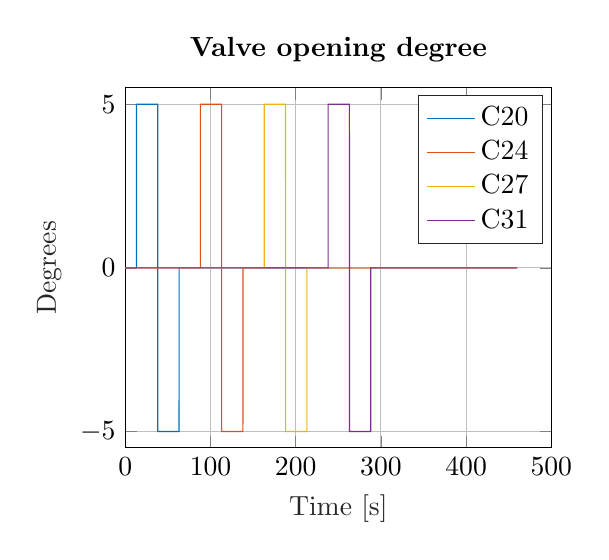
\begin{tikzpicture} %[scale=0.6,transform shape]

\begin{axis}[%
width=2.13in,
height=1.8in,
at={(0.758in,0.481in)},
scale only axis,
xmin=0,
xmax=500,
xlabel style={font=\color{white!15!black}},
xlabel={Time [s]},
ymin=-5.5,
ymax=5.5,
ylabel style={font=\color{white!15!black}},
ylabel={Degrees},
axis background/.style={fill=white},
title style={font=\bfseries},
title={Valve opening degree},
xmajorgrids,
ymajorgrids,
legend style={legend cell align=left, align=left, draw=white!15!black}
]
\addplot [color=mycolor1]
  table[row sep=crcr]{%
0	-1.13686837721616e-13\\
13.05	-1.13686837721616e-13\\
13.1	4.99999999999994\\
38.05	4.99999999999994\\
38.1	-5.00000000000006\\
63.05	-5.00000000000006\\
63.1	-1.13686837721616e-13\\
459.95	-1.13686837721616e-13\\
};
\addlegendentry{C20}

\addplot [color=mycolor2]
  table[row sep=crcr]{%
0	-1.13686837721616e-13\\
88.05	-1.13686837721616e-13\\
88.1	4.99999999999994\\
113.05	4.99999999999994\\
113.1	-5.00000000000006\\
138.05	-5.00000000000006\\
138.1	-1.13686837721616e-13\\
459.95	-1.13686837721616e-13\\
};
\addlegendentry{C24}

\addplot [color=mycolor3]
  table[row sep=crcr]{%
0	-1.13686837721616e-13\\
163.05	-1.13686837721616e-13\\
163.1	4.99999999999994\\
188.05	4.99999999999994\\
188.1	-5.00000000000006\\
213.05	-5.00000000000006\\
213.1	-1.13686837721616e-13\\
459.95	-1.13686837721616e-13\\
};
\addlegendentry{C27}

\addplot [color=mycolor4]
  table[row sep=crcr]{%
0	-1.13686837721616e-13\\
238.05	-1.13686837721616e-13\\
238.1	4.99999999999994\\
263.05	4.99999999999994\\
263.1	-5.00000000000006\\
288.05	-5.00000000000006\\
288.1	-1.13686837721616e-13\\
459.95	-1.13686837721616e-13\\
};
\addlegendentry{C31}

\end{axis}
\end{tikzpicture}% 
    \caption{Small-signal values of the opening degrees of the pma valves. }
    \label{fig:est_OD_data_w}
  \end{minipage}
  \hfill
  \begin{minipage}[b]{0.45\textwidth}
    % This file was created by matlab2tikz.
%
%The latest updates can be retrieved from
%  http://www.mathworks.com/matlabcentral/fileexchange/22022-matlab2tikz-matlab2tikz
%where you can also make suggestions and rate matlab2tikz.
%
\definecolor{mycolor1}{rgb}{0.00000,0.44700,0.74100}%
\definecolor{mycolor2}{rgb}{0.85000,0.32500,0.09800}%
%
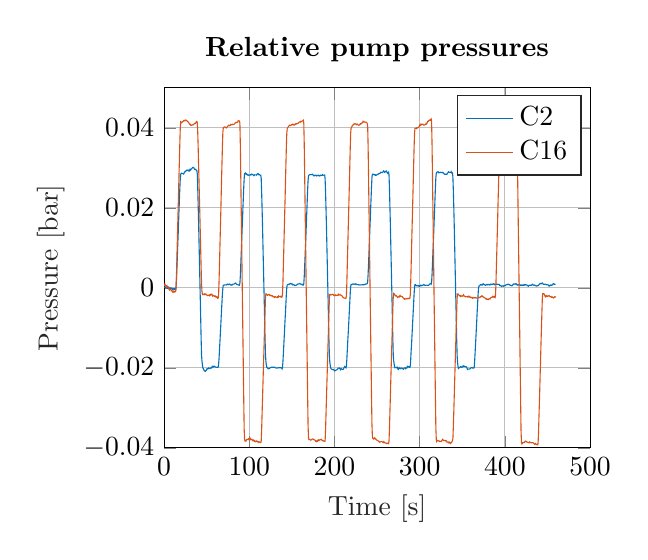
\begin{tikzpicture}

\begin{axis}[%
scaled y ticks = false,
 y tick label style={/pgf/number format/fixed,
/pgf/number format/1000 sep = \thinspace}, % Optional if you want to replace comma as the 1000 separator 
width=2.13in,
height=1.8in,
at={(0.758in,0.481in)},
scale only axis,
xmin=0,
xmax=500,
xlabel style={font=\color{white!15!black}},
xlabel={Time [s]},
ymin=-0.04,
ymax=0.05,
ylabel style={font=\color{white!15!black}},
ylabel={Pressure [bar]},
axis background/.style={fill=white},
title style={font=\bfseries},
title={Relative pump pressures},
xmajorgrids,
ymajorgrids,
legend style={legend cell align=left, align=left, draw=white!15!black}
]
\addplot [color=mycolor1]
  table[row sep=crcr]{%
0	0.000234573558145712\\
0.5	0.000142931329435214\\
1	0.000112383919827153\\
1.5	0.000191807184762638\\
2	7.57270283315847e-05\\
3.5	-1.59152003789131e-05\\
4	-0.000101447947201905\\
4.5	0.000124602883659009\\
5	0.00021624511242635\\
6	8.18365102759344e-05\\
6.5	-0.000150323802529329\\
7	-0.000217528103632958\\
7.5	-8.92289833700488e-05\\
8	-1.59152003789131e-05\\
8.5	-0.000113666911033761\\
9	-5.86815738188307e-05\\
9.5	-0.000309170332343456\\
10	-0.000425250488774509\\
11	-0.00030306085045595\\
11.5	-0.000125885874865617\\
12	-0.000131995356809966\\
12.5	-0.000406922042998303\\
13	-0.000443578934493871\\
13.5	-0.000333608260007168\\
14	0.000142931329435214\\
14.5	0.00181692937439948\\
15	0.00443789711630416\\
15.5	0.00732768206256651\\
16	0.0103518756109224\\
16.5	0.013174456256138\\
17	0.0161375549853346\\
17.5	0.0191922959432986\\
18	0.022082080889561\\
18.5	0.0248985520527754\\
19	0.0271896077712768\\
19.5	0.0283626282991349\\
20	0.0286375549853233\\
20.5	0.0286558834310995\\
21	0.0285886791299959\\
21.5	0.0285703506842765\\
22	0.0286131170576596\\
22.5	0.0284787084555092\\
23	0.0284603800097898\\
23.5	0.0287169782502588\\
24	0.0287841825513055\\
24.5	0.0290957661290463\\
25.5	0.0291446419843737\\
26	0.0293890212610108\\
26.5	0.0294256781525064\\
27	0.0293401454056834\\
28	0.0294562255620576\\
28.5	0.0293034885141878\\
29	0.029376802297179\\
29.5	0.0292301747311967\\
30.5	0.0296395100195355\\
31	0.0294501160801701\\
31.5	0.0295967436461524\\
32.5	0.0298166849951258\\
33.5	0.0301160496089778\\
34.5	0.0300793927174823\\
35	0.0299877504887718\\
35.5	0.0297372617301903\\
36	0.029590634164208\\
36.5	0.0295661962365443\\
37	0.029633400537648\\
38	0.0294012402248427\\
38.5	0.0293706928152346\\
39	0.0283992851906305\\
39.5	0.0250085227272621\\
40	0.0208662939882629\\
40.5	0.0165896566471133\\
41.5	0.00690001832845155\\
42	0.00201243279570917\\
42.5	-0.00279572947215456\\
43	-0.00765276759534572\\
43.5	-0.0126991996579022\\
44	-0.0168536473607332\\
44.5	-0.0183015945747798\\
45	-0.0192363453079452\\
45.5	-0.0199878115835759\\
46	-0.0201527675953344\\
46.5	-0.0204215847996352\\
47	-0.0206415261486086\\
48	-0.0208309200879739\\
48.5	-0.0208675769794695\\
49	-0.0207026209677679\\
49.5	-0.0206476356304961\\
50	-0.0203849279081396\\
50.5	-0.0202077529325493\\
51	-0.0201894244868299\\
51.5	-0.0202505193059892\\
52	-0.0200855632942307\\
52.5	-0.0199878115835759\\
53	-0.0201161107038388\\
53.5	-0.0201710960410537\\
54	-0.0201772055229981\\
54.5	-0.0200427969208477\\
55	-0.0200672348485114\\
55.5	-0.0200550158846795\\
56.5	-0.0196151331867327\\
57.5	-0.019847293499538\\
58	-0.0196090237047883\\
58.5	-0.0195662573314053\\
59	-0.0195723668132928\\
60	-0.0197984176442105\\
60.5	-0.0197739797165468\\
61.5	-0.0198961693548654\\
63.5	-0.0198289650537617\\
64	-0.0190897177419629\\
64.5	-0.0177517412023462\\
65	-0.0157417216520344\\
66	-0.0116544782502501\\
66.5	-0.00965667766371325\\
67	-0.00753668743891467\\
67.5	-0.00534949291301245\\
68	-0.00338834921797115\\
68.5	-0.00134778225805121\\
69	-0.000101447947201905\\
69.5	0.000631689882709452\\
70.5	0.000717222629532444\\
71	0.000686675219924382\\
71.5	0.000753879521028011\\
73	0.00072333211141995\\
73.5	0.000753879520971168\\
74	0.000955492424225213\\
74.5	0.000888288123121583\\
75	0.000869959677402221\\
75.5	0.000808864858242941\\
76	0.000894397605065933\\
77	0.000967711388057069\\
78	0.000735551075251806\\
78.5	0.000790536412466736\\
79	0.000686675219924382\\
79.5	0.000668346774148176\\
81	0.000924945014617151\\
82	0.000924945014617151\\
84	0.00120598118274984\\
84.5	0.00104713465293571\\
85	0.000924945014617151\\
86	0.000833302785906653\\
87	0.000753879520971168\\
87.5	0.000686675219924382\\
88	0.000729441593307456\\
88.5	0.000668346774148176\\
89	0.00117543377319862\\
89.5	0.00288608870965845\\
90	0.00569034090904097\\
90.5	0.00840295087971299\\
91	0.0111766556695443\\
91.5	0.0140481121700304\\
92	0.0167607221407025\\
92.5	0.0196505070869648\\
93.5	0.0250390701368133\\
94	0.0272934689637623\\
94.5	0.0285459127565559\\
95.5	0.0287291972140338\\
96.5	0.028417613636293\\
97	0.0284848179373967\\
97.5	0.0282526576245914\\
98	0.028203781769264\\
98.5	0.0282832050341426\\
99	0.0281610153958241\\
99.5	0.0281854533234878\\
100	0.0281610153958241\\
101	0.028203781769264\\
101.5	0.028289314516087\\
102	0.0282282196969277\\
102.5	0.0283809567447975\\
103	0.0284481610459011\\
103.5	0.0284053946724612\\
104	0.0283259714075825\\
104.5	0.0282098912511515\\
105.5	0.0280510447213373\\
106	0.0282648765884232\\
106.5	0.0282282196969277\\
108	0.0282587671064789\\
108.5	0.0281915628054321\\
109	0.0283442998533019\\
109.5	0.0285336937927241\\
110	0.0284848179373967\\
110.5	0.0285275843107797\\
111	0.0283198619256382\\
111.5	0.02837484726291\\
112.5	0.0281854533234878\\
113	0.0281610153958241\\
113.5	0.0281732343596559\\
114	0.0273362353372022\\
114.5	0.0241593047409197\\
115	0.0202370173508939\\
115.5	0.0160459127565673\\
116.5	0.00649068304005596\\
117	0.00199410434993297\\
117.5	-0.00275296309877149\\
118.5	-0.0124609298631526\\
119	-0.0165176258553288\\
119.5	-0.0183443609482197\\
120	-0.0192057978983371\\
120.5	-0.0198350745357061\\
121	-0.0198839503910335\\
121.5	-0.0200122495112396\\
122	-0.0202260813783255\\
122.5	-0.0202444098240449\\
123	-0.0202016434506618\\
123.5	-0.0200916727761751\\
124	-0.0200916727761751\\
124.5	-0.0199878115835759\\
126	-0.0198350745357061\\
127.5	-0.019847293499538\\
128	-0.0198839503910335\\
128.5	-0.0198778409090892\\
129	-0.0198106366080424\\
129.5	-0.019847293499538\\
130	-0.0198411840175936\\
130.5	-0.0199511546920803\\
132	-0.0200733443303989\\
132.5	-0.0200794538123432\\
134	-0.0199511546920803\\
134.5	-0.0200122495112396\\
136	-0.0199389357282485\\
136.5	-0.0199633736559122\\
137	-0.0199267167644166\\
138	-0.0200427969208477\\
138.5	-0.0202566287878767\\
139	-0.0199206072825291\\
139.5	-0.0185398643695294\\
140	-0.0165298448191606\\
141	-0.0123692876344421\\
142	-0.00806821236562882\\
142.5	-0.00606430229720445\\
143	-0.00395042155429337\\
143.5	-0.00167158479962382\\
144	-9.80571849140688e-06\\
144.5	0.000674456256092526\\
145	0.00077831744863488\\
145.5	0.000796645894411085\\
146	0.000894397605065933\\
146.5	0.000851631231626016\\
147	0.000876069159289727\\
147.5	0.000955492424225213\\
148	0.00112044843598369\\
149	0.00108379154448812\\
149.5	0.000961601906226406\\
150	0.000955492424282056\\
150.5	0.000986039833890118\\
151	0.000741660557252999\\
151.5	0.00077220796686106\\
152	0.000741660557309842\\
152.5	0.000766098484973554\\
153	0.000607251955159427\\
153.5	0.000576704545551365\\
154	0.000582814027495715\\
155	0.000668346774318707\\
155.5	0.000686675220038069\\
156	0.000790536412637266\\
156.5	0.000821083822188484\\
157	0.000961601906283249\\
157.5	0.000949382942451393\\
158	0.00100436827966632\\
159	0.000998258797778817\\
159.5	0.00108990102648932\\
160	0.0009554924243389\\
160.5	0.000912726050955825\\
161	0.000931054496675188\\
161.5	0.000888288123292114\\
162	0.000753879521141698\\
162.5	0.00083941226796469\\
163	0.000692784701982418\\
163.5	0.000680565738150563\\
164	0.00107768206265746\\
164.5	0.00271502321612616\\
165	0.00523823924743283\\
165.5	0.00788975439894557\\
166	0.0106268022972813\\
166.5	0.0132599890030178\\
167	0.0160703506843447\\
167.5	0.018844055474176\\
168.5	0.0244586693549422\\
169	0.0267924914468267\\
169.5	0.0278921981916938\\
170	0.0281671248778821\\
171	0.0283259714076962\\
171.5	0.0283137524438644\\
172	0.0283504093353599\\
173.5	0.028295423998145\\
174	0.0284053946726317\\
176	0.0279899499023486\\
176.5	0.028124358504499\\
177	0.0280877016130034\\
177.5	0.0281121395406672\\
178	0.0281793438417139\\
178.5	0.0281610153959946\\
179	0.0279838404204042\\
180.5	0.0281182490225547\\
181	0.0280693731672272\\
181.5	0.0281671248778821\\
182.5	0.0279655119746849\\
183	0.0279899499023486\\
183.5	0.0280571542033954\\
184	0.0281976722874902\\
184.5	0.0281304679863865\\
185	0.0280999205768353\\
185.5	0.0281365774683309\\
186	0.0282770955523688\\
186.5	0.0281487964321627\\
187	0.0281915628055458\\
188.5	0.0282037817693777\\
189	0.0273179068915965\\
189.5	0.0243364797166237\\
190	0.020371425953158\\
190.5	0.0162597446237669\\
191	0.0115310056208386\\
192.5	-0.00286293377308766\\
193	-0.00784216153459738\\
193.5	-0.012705309139676\\
194	-0.0167925525414034\\
194.5	-0.0185032074778633\\
195	-0.0192852211631021\\
195.5	-0.0199511546919666\\
196	-0.020226081378155\\
197.5	-0.0204215847994647\\
199	-0.0203788184260816\\
199.5	-0.0206231977027187\\
200	-0.0206720735580461\\
200.5	-0.0207759347505885\\
202	-0.020513227028232\\
203	-0.0204643511729046\\
203.5	-0.0203299425707542\\
204	-0.020256628787763\\
204.5	-0.020055015884509\\
205	-0.0200611253664533\\
205.5	-0.0200122495111259\\
206	-0.0201161107036683\\
206.5	-0.0201649865589957\\
207	-0.0204460227271284\\
207.5	-0.0202810667154267\\
208	-0.0201772055228275\\
208.5	-0.020311614124978\\
209	-0.0203665994622497\\
210	-0.0203543804984179\\
210.5	-0.0203177236069223\\
211	-0.0200305779568453\\
211.5	-0.0199083883185267\\
212	-0.0196884469695533\\
212.5	-0.0198656219451436\\
213	-0.0199083883185267\\
213.5	-0.0200061400291816\\
214	-0.019499053030188\\
214.5	-0.0179472446235422\\
215	-0.0158883492178461\\
215.5	-0.0137500305472713\\
216	-0.0118438721895018\\
216.5	-0.00988272849451732\\
218.5	-0.00137222018560124\\
219	0.000301777859363028\\
219.5	0.000845521749852196\\
220	0.000857740713684052\\
220.5	0.000796645894524772\\
221	0.00090050708712397\\
221.5	0.000967711388170756\\
222	0.000937163978619537\\
222.5	0.000967711388170756\\
223	0.000912726050955825\\
223.5	0.000949382942451393\\
224	0.00090050708712397\\
224.5	0.00090050708712397\\
225	0.00101047776161067\\
225.5	0.000967711388170756\\
226	0.000869959677515908\\
226.5	0.000814974340300978\\
229.5	0.000753879521141698\\
230	0.000698894183869925\\
230.5	0.000747770039197349\\
233.5	0.00077831744880541\\
234	0.000747770039197349\\
234.5	0.000808864858356628\\
235	0.00083330278602034\\
235.5	0.000796645894524772\\
236.5	0.000949382942451393\\
237.5	0.00101047776161067\\
238	0.000986039833946961\\
238.5	0.00110822947226552\\
239	0.0015847690617079\\
239.5	0.00343594208220566\\
240	0.00603858137839097\\
240.5	0.00878784824055856\\
241	0.0115737719942217\\
242	0.0170723057185569\\
242.5	0.0199743096286511\\
243	0.022613605816332\\
243.5	0.025326215787004\\
244	0.0275989430597292\\
244.5	0.0283992851906874\\
245	0.0283992851906874\\
245.5	0.0283381903715281\\
246	0.0283931757087998\\
246.5	0.0283626282991918\\
247	0.028295423998145\\
247.5	0.0281854533236583\\
248	0.0282770955523688\\
248.5	0.0281487964321627\\
249	0.0281549059140502\\
250.5	0.0283870662268555\\
251	0.0283626282991918\\
251.5	0.0284970369013422\\
252	0.0285581317205015\\
252.5	0.028552022238614\\
253.5	0.0286253360216051\\
254	0.0288880437439616\\
255	0.0288147299609705\\
255.5	0.0288574963344104\\
256	0.0288269489248023\\
256.5	0.0288636058162979\\
257	0.0290163428642245\\
257.5	0.0292362842131979\\
258.5	0.029107985092935\\
259	0.0288758247801297\\
259.5	0.0289613575269527\\
260	0.029193517839758\\
260.5	0.0291874083578705\\
261	0.0292179557674217\\
261.5	0.028936919599289\\
262	0.0288208394429148\\
262.5	0.0286314455034926\\
263	0.0287414161779793\\
263.5	0.0288880437439616\\
264	0.0283198619258087\\
264.5	0.0253078873412278\\
265	0.0210984543011818\\
265.5	0.0168218169600323\\
266	0.0119831072826173\\
266.5	0.00723603983391286\\
267	0.00223848362668377\\
267.5	-0.00267353983372232\\
268	-0.00770775293244697\\
268.5	-0.012589228983245\\
269	-0.0168047715052353\\
269.5	-0.0182221713097306\\
270	-0.0189369806939226\\
270.5	-0.0197434323068251\\
271	-0.019969483137686\\
272	-0.0199144978004711\\
272.5	-0.0199755926196303\\
273	-0.0198717314270311\\
273.5	-0.0198106366078719\\
274	-0.0198472934993674\\
274.5	-0.0203238330888098\\
275	-0.0203910373899134\\
275.5	-0.0201527675951638\\
276	-0.019969483137686\\
276.5	-0.0201100012217807\\
277.5	-0.0202016434504912\\
278.5	-0.0200122495111259\\
279	-0.0200611253664533\\
279.5	-0.02017109604094\\
281	-0.0203299425707542\\
281.5	-0.0201100012217807\\
282	-0.0200122495111259\\
283	-0.0199878115834622\\
283.5	-0.0202016434504912\\
284	-0.0200916727760045\\
284.5	-0.0200366874387896\\
285	-0.0200305779568453\\
285.5	-0.0196029142227303\\
286	-0.0196151331865622\\
286.5	-0.01979841764404\\
287	-0.0197678702344888\\
287.5	-0.0196823374876658\\
288	-0.0198717314270311\\
288.5	-0.0198534029813118\\
289	-0.0195112719940198\\
289.5	-0.0178556023947749\\
290	-0.0157417216518638\\
290.5	-0.0140616141250121\\
291.5	-0.00980941471152619\\
292	-0.00770164345050262\\
292.5	-0.00564885752675082\\
293	-0.00348610092851231\\
293.5	-0.00143331500476052\\
294	0.000179588221044469\\
294.5	0.000802755376469122\\
295	0.000796645894524772\\
296	0.000570595063663859\\
296.5	0.000588923509383221\\
297	0.000485062316840867\\
297.5	0.000540047654055797\\
298	0.000497281280672723\\
298.5	0.000588923509383221\\
299	0.000582814027495715\\
299.5	0.00038120112424167\\
300	0.000375091642354164\\
300.5	0.000478952834896518\\
301	0.000662237292374357\\
302	0.000662237292374357\\
302.5	0.000527828690223942\\
303.5	0.000607251955159427\\
304.5	0.000808864858299785\\
305	0.000766098484859867\\
305.5	0.000759989002915518\\
306	0.000625580400765102\\
306.5	0.000625580400708259\\
307	0.000588923509212691\\
307.5	0.000674456255978839\\
308	0.000692784701698201\\
309	0.000637799364426428\\
309.5	0.000595032991043354\\
310	0.000631689882538922\\
310.5	0.000625580400594572\\
311.5	0.000876069159176041\\
312.5	0.00106546309854139\\
313	0.00102880620704582\\
313.5	0.000943273460222827\\
314	0.00140148460394585\\
314.5	0.0032526576244436\\
315	0.00584307795679706\\
315.5	0.00848237414447794\\
316	0.0112133125609262\\
316.5	0.013822061338999\\
317	0.0167118462852613\\
318	0.0223142412021389\\
318.5	0.0252162451122331\\
319	0.0275745051317813\\
319.5	0.0285764601659935\\
320	0.0288574963341262\\
320.5	0.0289491385628367\\
321	0.0289491385628367\\
321.5	0.029040780791604\\
322	0.0289674670086129\\
322.5	0.0287597446234713\\
323	0.0288208394426306\\
323.5	0.0288269489245181\\
324	0.0288941532256217\\
324.5	0.0288880437436774\\
325	0.0288330584064624\\
325.5	0.0288574963341262\\
326	0.0288391678883499\\
326.5	0.0288941532256217\\
327	0.0287780730691907\\
327.5	0.0288208394426306\\
328	0.028668102394704\\
328.5	0.0286008980936572\\
329	0.028411504154235\\
329.5	0.0284420515638431\\
330	0.0283931757085156\\
331	0.028411504154235\\
331.5	0.0284420515638431\\
332	0.0284176136361793\\
332.5	0.0286864308404802\\
333	0.0287414161776951\\
334	0.0290102333819959\\
334.5	0.0288941532256217\\
335	0.0288513868521818\\
336	0.0288758247798455\\
336.5	0.0288819342617899\\
337	0.0290529997554358\\
337.5	0.0287658541053588\\
338	0.0288513868521818\\
338.5	0.0286864308404802\\
339	0.0277211326977636\\
339.5	0.0245136546918729\\
340	0.0206341336752871\\
340.5	0.016320839442642\\
341	0.0114393633917871\\
341.5	0.00636238391967936\\
342	0.00145646994116078\\
342.5	-0.00338223973625418\\
343	-0.00836146749770705\\
343.5	-0.0132307245847301\\
344	-0.0170674792279328\\
344.5	-0.0186559445260741\\
345	-0.0196212426687907\\
345.5	-0.0201649865592799\\
346	-0.0200733443305694\\
346.5	-0.0199144978007553\\
347.5	-0.0198411840177641\\
348	-0.0196884469698375\\
348.5	-0.0196762280060057\\
349	-0.0198350745358198\\
349.5	-0.0198900598730916\\
350	-0.0198228555719879\\
350.5	-0.0196456805964544\\
351	-0.019511271994304\\
351.5	-0.0196334616326226\\
352	-0.0195540383676871\\
352.5	-0.0196029142230145\\
353	-0.0197006659336694\\
354	-0.0197373228251649\\
354.5	-0.0197189943794456\\
355	-0.0197739797166605\\
355.5	-0.0200305779571295\\
356	-0.0203788184263658\\
356.5	-0.0202871761975985\\
357.5	-0.020323833089094\\
358	-0.020323833089094\\
359	-0.0202321908603835\\
359.5	-0.0201772055231118\\
360.5	-0.019938935728419\\
361.5	-0.0199144978007553\\
362	-0.0200366874390738\\
363	-0.0200000305475783\\
363.5	-0.0200550158847932\\
364	-0.019853402981596\\
364.5	-0.0184726600685963\\
366.5	-0.0103714870480758\\
367.5	-0.00602153592393506\\
368.5	-0.0018854166668234\\
369	-0.000205309139971632\\
369.5	0.000448405425061083\\
370.5	0.00054004765377158\\
371	0.000735551075081275\\
371.5	0.000845521749567979\\
372	0.000839412267680473\\
372.5	0.000729441593193769\\
373.5	0.000729441593193769\\
374	0.000931054496390971\\
374.5	0.00103491568899017\\
375	0.000918835532559115\\
375.5	0.000863850195344185\\
376	0.000845521749567979\\
376.5	0.000711113147417564\\
377	0.000619470918707066\\
377.5	0.000656127810202634\\
378.5	0.000857740713399835\\
379	0.000869959677231691\\
379.5	0.000747770038913131\\
380	0.000778317448521193\\
380.5	0.000882178641063547\\
381	0.000876069159176041\\
381.5	0.000766098484689337\\
382	0.00072333211124942\\
383	0.000918835532559115\\
383.5	0.000808864858072411\\
384.5	0.000918835532559115\\
385	0.000949382942167176\\
385.5	0.000851631231512329\\
386	0.000851631231512329\\
387	0.00104102517087767\\
387.5	0.000967711387886538\\
388	0.000784426930408699\\
388.5	0.000821083821904267\\
389	0.000912726050671608\\
389.5	0.000839412267680473\\
390.5	0.000918835532559115\\
393.5	0.000851631231512329\\
394	0.000564485581435292\\
394.5	0.000588923509099004\\
395	0.000576704545267148\\
395.5	0.000497281280388506\\
396	0.000362872678238091\\
396.5	0.000472843352724794\\
397.5	0.00048506231655665\\
398.5	0.000411748533565515\\
399	0.000527828689939724\\
399.5	0.000497281280388506\\
400	0.000503390762276013\\
400.5	0.000595032991043354\\
401	0.000735551075081275\\
401.5	0.000766098484689337\\
402.5	0.000784426930408699\\
403	0.000833302785736123\\
403.5	0.000924945014503464\\
405	0.000863850195344185\\
405.5	0.000766098484689337\\
406	0.000729441593193769\\
406.5	0.000619470918707066\\
407.5	0.000564485581435292\\
408	0.000515609726107868\\
408.5	0.000576704545267148\\
409	0.000582814027211498\\
409.5	0.000845521749567979\\
410	0.000876069159176041\\
410.5	0.00099214931555025\\
411	0.000961601905999032\\
411.5	0.000986039833662744\\
412	0.000924945014503464\\
412.5	0.00101658724321396\\
413	0.00104102517087767\\
413.5	0.000955492424054682\\
414	0.000924945014503464\\
414.5	0.000686675219753852\\
415	0.000802755376184905\\
415.5	0.000741660557025625\\
416	0.000717222629361913\\
416.5	0.000772207966576843\\
417	0.000876069159176041\\
417.5	0.000705003665530057\\
418	0.000741660557025625\\
418.5	0.000582814027211498\\
419	0.000582814027211498\\
419.5	0.000705003665530057\\
420	0.000619470918707066\\
420.5	0.000595032991043354\\
421	0.000717222629361913\\
421.5	0.00066834677403449\\
422	0.00066223729209014\\
422.5	0.000784426930408699\\
423	0.000680565737866345\\
423.5	0.000833302785736123\\
424	0.000851631231512329\\
424.5	0.000753879520857481\\
425	0.000711113147417564\\
425.5	0.000753879520857481\\
426	0.000686675219753852\\
427	0.000497281280388506\\
427.5	0.000417858015453021\\
428	0.000582814027211498\\
428.5	0.00060114247293086\\
429	0.000674456255921996\\
429.5	0.000643908846370778\\
430	0.000692784701698201\\
431	0.000637799364426428\\
431.5	0.000698894183585708\\
432	0.000882178641063547\\
432.5	0.000918835532559115\\
433	0.000747770038913131\\
434	0.000637799364426428\\
434.5	0.000735551075081275\\
435.5	0.000631689882538922\\
436	0.000552266617603436\\
436.5	0.000515609726107868\\
437	0.000442295943116733\\
437.5	0.000472843352724794\\
438	0.000552266617603436\\
438.5	0.00054004765377158\\
439	0.000619470918707066\\
439.5	0.00060725195487521\\
440	0.000766098484689337\\
440.5	0.000869959677231691\\
441	0.00101658724321396\\
441.5	0.0011082294719813\\
442	0.00099214931555025\\
442.5	0.00099214931555025\\
443	0.00104713465282202\\
443.5	0.00118154325497244\\
444	0.00123041911029986\\
445	0.000931054496390971\\
445.5	0.000869959677231691\\
446.5	0.000863850195344185\\
447	0.000943273460222827\\
447.5	0.000949382942167176\\
448	0.000912726050671608\\
448.5	0.000790536412353049\\
449	0.000772207966576843\\
449.5	0.000790536412353049\\
451	0.000711113147417564\\
451.5	0.000527828689939724\\
452	0.000436186461229227\\
452.5	0.000491171798444157\\
453	0.00066223729209014\\
453.5	0.000717222629361913\\
454	0.000595032991043354\\
454.5	0.000686675219753852\\
455	0.000650018328258284\\
455.5	0.000753879520857481\\
456	0.000741660557025625\\
456.5	0.000986039833662744\\
457	0.00104102517087767\\
457.5	0.00101047776132646\\
458	0.000888288123007897\\
458.5	0.000912726050671608\\
459.5	0.000863850195344185\\
};
\addlegendentry{C2}

\addplot [color=mycolor2]
  table[row sep=crcr]{%
0	0.000453720674499891\\
0.5	0.00063700513197773\\
1	0.000930260263942273\\
1.5	0.00069809995113701\\
2	0.000575910312818451\\
2.5	0.000545362903210389\\
3	0.00030098362657327\\
3.5	0.000496487047882965\\
4	0.000227669843582134\\
4.5	0.00024599828935834\\
5	8.71517595442128e-05\\
5.5	-0.000230541300084042\\
6.5	-0.00054212487782479\\
7	-0.000389387829898169\\
8	-0.000340511974570745\\
8.5	-0.000707080889526424\\
9	-0.000670423998030856\\
10	-0.00101255498532282\\
10.5	-0.000908693792780468\\
11	-0.00104921187681839\\
11.5	-0.000829270527844983\\
12	-0.00104310239493088\\
12.5	-0.00104921187681839\\
13	-0.000969788611939748\\
13.5	-0.000945350684276036\\
14	-0.000395497311842519\\
14.5	0.00257371089929848\\
15	0.0069480999511029\\
15.5	0.0111758614369251\\
16	0.0155074841153464\\
16.5	0.0195458516617464\\
17	0.0237797226295129\\
17.5	0.0279402798142314\\
18	0.0319786473606882\\
18.5	0.0361819709188467\\
19	0.0399576307428902\\
19.5	0.0414911107038165\\
20.5	0.041283388318675\\
22	0.0416316287878544\\
22.5	0.0416316287878544\\
23.5	0.0418821175464359\\
24	0.041839351172996\\
24.5	0.0417415994623411\\
25	0.0419309934017633\\
25.5	0.041955431329427\\
26	0.041924883919819\\
26.5	0.0418576796187722\\
27	0.0417354899804536\\
28	0.0415583150048633\\
28.5	0.0413750305473855\\
29	0.0413200452101705\\
29.5	0.0410573374877572\\
30	0.0409107099217749\\
30.5	0.0409595857771023\\
31	0.0407213159824096\\
31.5	0.0406235642717547\\
32	0.0406907685728015\\
32.5	0.0406480021994184\\
33.5	0.0407946297654007\\
34	0.0408129582111201\\
34.5	0.0407824108015689\\
35	0.0409107099217749\\
35.5	0.0410817754154209\\
36	0.0410817754154209\\
36.5	0.0411795271260758\\
37	0.0411673081622439\\
37.5	0.0414177969208254\\
38	0.0415888624144714\\
38.5	0.0416010813783032\\
39	0.0412467314271794\\
39.5	0.0389617851906223\\
40	0.0353755193059442\\
40.5	0.0309644733626442\\
41	0.0267122739491583\\
41.5	0.0223501038611857\\
42	0.0182445320136821\\
42.5	0.0138029386608309\\
43	0.00941633064519465\\
43.5	0.00496251832845473\\
44	0.000979136119269697\\
44.5	-0.000914803274667975\\
45	-0.00167848851413055\\
45.5	-0.00171514540562612\\
46	-0.0015807368034757\\
46.5	-0.00156240835775634\\
47	-0.00162961265880313\\
47.5	-0.00151964198431642\\
48	-0.00167237903224304\\
48.5	-0.00152575146626077\\
49	-0.00153797043009263\\
49.5	-0.00171514540562612\\
51	-0.00192897727271202\\
51.5	-0.00182511608011282\\
52	-0.00181289711628096\\
52.5	-0.00189232038121645\\
53	-0.00180067815244911\\
53.5	-0.00197174364609509\\
54	-0.00183122556205717\\
54.5	-0.00164183162263498\\
55	-0.00176402126095354\\
55.5	-0.00170903592373861\\
56	-0.00158684628542005\\
56.5	-0.00172736436945797\\
57	-0.00205116691103058\\
57.5	-0.00196563416420759\\
58	-0.0019900720918713\\
58.5	-0.00192286779076767\\
59	-0.00211837121207736\\
59.5	-0.00211226173018986\\
60	-0.00204505742908623\\
60.5	-0.00203283846525437\\
61	-0.00233831256110761\\
62	-0.00225277981428462\\
62.5	-0.00253992546430482\\
63	-0.0026193487292403\\
63.5	-0.00256436339202537\\
64	-0.00161739369502811\\
64.5	0.00143123778099152\\
65	0.00547571480933584\\
65.5	0.00965460043988742\\
66	0.0139495662267564\\
66.5	0.0181834371945229\\
67.5	0.0271460471652176\\
68	0.0314349034701991\\
68.5	0.0354488330889922\\
69	0.0389006903715199\\
69.5	0.0399881781525551\\
70	0.0401164772727611\\
71	0.0402386669110797\\
71.5	0.040244776393024\\
72	0.0401653531280886\\
72.5	0.0400309445259381\\
73	0.0399881781525551\\
73.5	0.0401409152004248\\
74	0.0401775720919204\\
75	0.0405197030792124\\
76	0.0406846590909709\\
76.5	0.0406480021994753\\
77	0.0405319220430442\\
77.5	0.0405991263441479\\
78	0.0407029875366902\\
78.5	0.0408801625122805\\
79	0.040757972873962\\
79.5	0.0407763013196814\\
80	0.0408740530303362\\
80.5	0.0409046004399443\\
81	0.0408251771750088\\
81.5	0.0408740530303362\\
82	0.0408740530303362\\
83	0.0410817754154778\\
83.5	0.0412711693548999\\
84.5	0.0414116874389379\\
85	0.0413078262463955\\
85.5	0.0413261546921149\\
86	0.0414055779570504\\
86.5	0.0415277675953689\\
87	0.0418088037635016\\
87.5	0.0417293804985661\\
88	0.0417599279081742\\
88.5	0.0416621761975193\\
89	0.0411611986804132\\
89.5	0.0359070442327152\\
90	0.028337396138852\\
90.5	0.0203217558651545\\
91	0.012489400048878\\
91.5	0.00446765029329299\\
92	-0.00360297531767628\\
92.5	-0.0115453018083826\\
93	-0.0196770222385112\\
93.5	-0.027698771994153\\
94	-0.0352073252688569\\
94.5	-0.0379565921310245\\
95	-0.0382865041544846\\
95.5	-0.0382559567448766\\
96	-0.0383353800098121\\
96.5	-0.0380176869501838\\
97	-0.0379260447214165\\
98	-0.0378893878299209\\
98.5	-0.0379688110948564\\
99	-0.0377244318182193\\
99.5	-0.0377183223362749\\
100	-0.0378282930107616\\
101	-0.0376022421799007\\
101.5	-0.0379504826490802\\
102	-0.0379871395405758\\
103	-0.037834402492706\\
103.5	-0.0379138257575846\\
104	-0.0382009714076617\\
104.5	-0.0382376282991572\\
105	-0.038048234359735\\
105.5	-0.0381215481427262\\
106	-0.0383537084555314\\
106.5	-0.0382376282991572\\
107.5	-0.03847589809385\\
108	-0.0384392412023544\\
108.5	-0.0382803946725403\\
109	-0.0383414894916996\\
109.5	-0.0383475989736439\\
110.5	-0.0386286351417766\\
111	-0.03847589809385\\
111.5	-0.0385431023949536\\
112	-0.0385064455034581\\
112.5	-0.0386286351417766\\
113	-0.0386714015151597\\
113.5	-0.038677510997104\\
114	-0.038304832600204\\
114.5	-0.035708302785963\\
115	-0.0318410007331522\\
116.5	-0.0207522910557714\\
117	-0.017135477761542\\
117.5	-0.0133598179374985\\
118.5	-0.00611397238520794\\
119	-0.00257658235585723\\
119.5	-0.00148909457482205\\
120	-0.00157462732164504\\
120.5	-0.00161128421314061\\
121	-0.00170903592379545\\
121.5	-0.00185566348977773\\
122	-0.00181900659828216\\
122.5	-0.00168459799613174\\
123	-0.00162350317697246\\
123.5	-0.00170292644190795\\
124	-0.00186177297172208\\
124.5	-0.00182511608022651\\
125.5	-0.00201451001959185\\
126	-0.0020206195015362\\
126.5	-0.00192286779088136\\
127	-0.00195341520043257\\
128	-0.00221001344090155\\
128.5	-0.00213669965791041\\
129	-0.00216724706751847\\
129.5	-0.00239940738032374\\
130.5	-0.00221001344090155\\
131	-0.0022222324047334\\
131.5	-0.00233831256116446\\
132	-0.00241162634415559\\
132.5	-0.00242995478987496\\
133	-0.00227110826006083\\
133.5	-0.00239329789837939\\
134	-0.00231998411538825\\
134.5	-0.00202672898342371\\
135	-0.00217335654940598\\
136	-0.00222834188667775\\
136.5	-0.00226499877817332\\
137	-0.00208782380258299\\
137.5	-0.00213669965791041\\
138	-0.00233831256110761\\
138.5	-0.00227721774194833\\
139	-0.00153186094820512\\
139.5	0.00130904814272981\\
140	0.00528632087002734\\
140.5	0.00939189271753094\\
141	0.013546340420362\\
141.5	0.0178596346530639\\
142	0.0219896444282313\\
143	0.0307262035680083\\
143.5	0.034990621945326\\
144	0.0384852456012368\\
144.5	0.0396827040567587\\
145	0.0399881781525551\\
146	0.0403119806940708\\
146.5	0.0404952651515487\\
147.5	0.0406907685728584\\
148	0.0406602211633071\\
148.5	0.0405746884164842\\
149	0.0406113453079797\\
149.5	0.0407763013196814\\
150	0.0408312866569531\\
150.5	0.0408129582111769\\
151	0.040929038367608\\
151.5	0.0407763013196814\\
152	0.0408373961388406\\
152.5	0.0406846590909709\\
153	0.0407335349462983\\
154	0.0409779142229354\\
154.5	0.0408923814761124\\
155	0.0409473668133273\\
155.5	0.0410451185239822\\
156	0.0410328995601503\\
156.5	0.041100103861254\\
157	0.041100103861254\\
157.5	0.0412100745357407\\
158	0.0413689210655548\\
159.5	0.0415094391495927\\
160	0.0414544538123778\\
160.5	0.0416194098240794\\
161	0.0415338770772564\\
162	0.0417110520528468\\
163	0.0417660373900617\\
163.5	0.0418821175464927\\
164	0.041100103861254\\
164.5	0.0362064088465672\\
165	0.0288628115836218\\
165.5	0.0207372006354376\\
166	0.0129415017107135\\
166.5	0.00510303641260634\\
167.5	-0.0108121639784144\\
168	-0.0187483809871765\\
168.5	-0.0268862108991925\\
169	-0.0342298081621379\\
169.5	-0.0374189577222523\\
170	-0.0378954973116947\\
170.5	-0.0378588404201992\\
171.5	-0.0379810300585177\\
172	-0.0380665628053407\\
172.5	-0.0379993585042939\\
173	-0.0379932490223496\\
173.5	-0.0379138257574709\\
174	-0.0377610887095443\\
174.5	-0.0377549792276568\\
175	-0.0378344024925354\\
176	-0.0378954973116947\\
176.5	-0.0380482343596213\\
177.5	-0.0381093291787806\\
178	-0.0383414894915859\\
179	-0.0384575696479601\\
179.5	-0.038243737780931\\
180	-0.0383353800096415\\
180.5	-0.0381093291787806\\
181	-0.0381887524436593\\
181.5	-0.0379749205766302\\
182	-0.0380054679861814\\
182.5	-0.0380848912511169\\
183	-0.0379810300585177\\
184	-0.0378893878298072\\
184.5	-0.0379504826489665\\
185	-0.0378954973116947\\
185.5	-0.0381704239979399\\
186.5	-0.0382498472628185\\
187	-0.0382192998532673\\
187.5	-0.0382926136362585\\
188	-0.0384025843107452\\
188.5	-0.0383903653469133\\
189	-0.0382742851904823\\
189.5	-0.0358182734602792\\
190	-0.0321525843107224\\
190.5	-0.0283341581132959\\
191.5	-0.0210577651513972\\
192	-0.0174104044476167\\
192.5	-0.0136897299607881\\
193.5	-0.00640111803511445\\
194	-0.00283318059621251\\
194.5	-0.00170903592368177\\
195	-0.00162350317685878\\
195.5	-0.00177013074284105\\
196.5	-0.00173347385134548\\
197	-0.00166016006835434\\
198	-0.00160517473108257\\
199	-0.00181289711622412\\
199.5	-0.00191675830882332\\
200	-0.00189842986304711\\
200.5	-0.00180067815239227\\
201	-0.00175180229706484\\
201.5	-0.00194730571837454\\
203	-0.00183733504388783\\
203.5	-0.00191064882687897\\
204	-0.00182511608005598\\
204.5	-0.00160517473108257\\
205	-0.00178845918856041\\
205.5	-0.00180678763433662\\
206	-0.00174569281517734\\
206.5	-0.00164794110452249\\
207	-0.00178845918856041\\
208.5	-0.00188621089921526\\
209.5	-0.00229554618761085\\
210	-0.00231998411527456\\
210.5	-0.0023932978982657\\
211	-0.00250937805463991\\
212.5	-0.00257658235574354\\
213	-0.00265600562062218\\
213.5	-0.00260102028340725\\
214	-0.0019839626098701\\
214.5	0.00101579301082211\\
215	0.00529853983391604\\
216	0.0135157930108107\\
216.5	0.0177068976051373\\
217	0.0218307978984171\\
217.5	0.0260096835289119\\
218	0.030494043255203\\
218.5	0.0348501038612312\\
219	0.0386257636852747\\
219.5	0.039957630742947\\
220	0.04004316348977\\
220.5	0.0403608565493983\\
221	0.0405441410068761\\
221.5	0.0405746884164842\\
222	0.040843505620785\\
222.5	0.0409534762952717\\
223	0.0409046004399443\\
223.5	0.0410084616324866\\
224	0.0410390090420947\\
224.5	0.0410206805963185\\
225	0.0409351478494955\\
225.5	0.0407946297654576\\
226	0.0409412573314398\\
226.5	0.0409901331867673\\
227	0.0408557245846168\\
227.5	0.0407701918377938\\
228	0.0407396444281858\\
228.5	0.0406296737536991\\
229.5	0.040757972873962\\
230	0.0409779142229354\\
230.5	0.0410328995601503\\
231	0.0409534762952717\\
232	0.0411489797165814\\
232.5	0.0412772788367874\\
233	0.0413444831378911\\
233.5	0.0416010813783601\\
234	0.0414788917400415\\
234.5	0.0415888624145282\\
235	0.0414727822580971\\
235.5	0.0415033296677052\\
236	0.0414483443304334\\
236.5	0.0414361253666016\\
237	0.0413811400293866\\
237.5	0.0414055779570504\\
238	0.0412956072825637\\
238.5	0.0410756659335902\\
239	0.0402508858749115\\
239.5	0.0353205339687861\\
240	0.0279402798143451\\
240.5	0.0200040628055262\\
241	0.0123305535191207\\
241.5	0.00427825635392765\\
242	-0.00367628910061057\\
242.5	-0.0115697397359895\\
243	-0.0192493585042826\\
243.5	-0.0271916849949889\\
244	-0.0341137280057637\\
244.5	-0.0371257025902878\\
245	-0.0376327895893382\\
245.5	-0.0376205706255064\\
246	-0.0377610887095443\\
247	-0.037486162023356\\
247.5	-0.0375594758063471\\
248	-0.0378038550829842\\
248.5	-0.037785526637208\\
249.5	-0.0380299059138451\\
250.5	-0.0381398765883318\\
251	-0.0382315188170992\\
251.5	-0.0382803946724266\\
252	-0.0384086937926327\\
252.5	-0.0383964748288008\\
253	-0.0385980877320549\\
253.5	-0.0384942265394557\\
254	-0.0385064455032875\\
254.5	-0.0384086937926327\\
255	-0.0384392412022407\\
255.5	-0.0384331317202964\\
256	-0.0384820075756238\\
256.5	-0.0386041972139424\\
257	-0.0386041972139424\\
257.5	-0.038671401515046\\
258	-0.0384453506841282\\
258.5	-0.0386530730692698\\
259	-0.0386836204788779\\
259.5	-0.0387813721895327\\
260	-0.0387813721895327\\
261	-0.0389157807916831\\
261.5	-0.0388546859725238\\
263	-0.038842467008692\\
263.5	-0.038927999755515\\
264	-0.0383964748288008\\
264.5	-0.0355494562559784\\
265	-0.0317860153957668\\
265.5	-0.028065340908995\\
266	-0.0240147543987064\\
266.5	-0.0202146566469992\\
267	-0.0166039528347142\\
267.5	-0.0129382636851574\\
268.5	-0.00541749144662163\\
269	-0.00223445136845157\\
269.5	-0.00137912390022166\\
270	-0.00144632820126844\\
270.5	-0.00155629887575515\\
271	-0.00181289711622412\\
271.5	-0.00199618157370196\\
272	-0.00202061950136567\\
272.5	-0.00195952468220639\\
273	-0.0020878238024693\\
273.5	-0.00214891862162858\\
274	-0.00238718841632135\\
275	-0.00230165566949836\\
275.5	-0.00216724706734794\\
276	-0.00226499877800279\\
276.5	-0.00203894794714188\\
277	-0.00190453934499146\\
277.5	-0.00212448069396487\\
278	-0.00213669965779673\\
278.5	-0.00210615224818866\\
279.5	-0.00219168499501166\\
280	-0.00229554618761085\\
280.5	-0.0024849401269762\\
281	-0.00254603494613548\\
282	-0.00282707111426816\\
282.5	-0.00272931940361332\\
283	-0.00282096163238066\\
283.5	-0.00282096163238066\\
284	-0.00265600562062218\\
284.5	-0.00275375733127703\\
285.5	-0.00273542888555767\\
286	-0.00262545821107096\\
286.5	-0.0025949108014629\\
287	-0.00263156769295847\\
287.5	-0.00273542888555767\\
288.5	-0.0025888013195754\\
289	-0.00170292644173742\\
289.5	0.0014067998534415\\
290	0.00548793377322454\\
290.5	0.00987454178886082\\
291	0.0141633980937854\\
291.5	0.0182811889051209\\
292	0.0225272788366624\\
293	0.0311905241933914\\
293.5	0.0353694098238293\\
294	0.0386807490222623\\
294.5	0.0398354411043442\\
296	0.0400003971161027\\
296.5	0.0398110031766805\\
297	0.0399454117788309\\
297.5	0.0400248350437664\\
298.5	0.0401164772724769\\
299	0.0401714626097487\\
299.5	0.0403975134406096\\
300	0.0407152065002379\\
300.5	0.0406052358257512\\
301	0.0405930168619193\\
301.5	0.0409656952588193\\
302	0.0409412573311556\\
302.5	0.0408068487290052\\
303	0.0409229288853794\\
303.5	0.0409473668130431\\
304	0.04090460043966\\
304.5	0.0407396444279016\\
305	0.0406724401268548\\
305.5	0.0407457539098459\\
306	0.0407518633917334\\
306.5	0.0408190676928371\\
307	0.0408312866566689\\
307.5	0.0410939943790254\\
308	0.0409779142226512\\
308.5	0.0410939943790254\\
309.5	0.0416560667152908\\
310	0.0416316287876271\\
310.5	0.0417904753174412\\
311.5	0.0418637891004323\\
312	0.0419920882206952\\
312.5	0.0419248839195916\\
313	0.0421142778590138\\
313.5	0.0422425769792198\\
314	0.0415338770769722\\
314.5	0.0362858321112185\\
315	0.0287956072822908\\
315.5	0.0206089015149473\\
316	0.0124894000486506\\
316.5	0.00446765029306562\\
317	-0.00364574169128673\\
317.5	-0.0114903164713382\\
318	-0.0194448619258765\\
318.5	-0.0276865530304917\\
319	-0.0350118218476609\\
319.5	-0.0378832783481471\\
320	-0.038353708455702\\
320.5	-0.0381154386609524\\
321	-0.0381215481428967\\
321.5	-0.0382376282992709\\
322	-0.0382131903716072\\
323	-0.0383720369014213\\
323.5	-0.0382987231184302\\
324	-0.038439241202525\\
324.5	-0.0384453506844125\\
325.5	-0.0383353800099258\\
327	-0.0378527309385959\\
327.5	-0.0379810300588019\\
328	-0.0381643145162798\\
329.5	-0.0381276576247842\\
330	-0.0381520955524479\\
330.5	-0.0382803946727108\\
331	-0.0383170515642064\\
331.5	-0.0382620662269346\\
332	-0.0385797592865629\\
333	-0.0385858687685072\\
333.5	-0.0387080584068258\\
334	-0.0385858687685072\\
334.5	-0.0387141678887133\\
335	-0.0385980877323391\\
335.5	-0.0387508247802089\\
336	-0.0387141678887133\\
336.5	-0.0388974523461911\\
337	-0.0386836204791621\\
338	-0.0384453506844125\\
338.5	-0.0382376282992709\\
339	-0.0377427602641092\\
339.5	-0.0349507270285017\\
340	-0.0314377749268715\\
341	-0.0240147543989906\\
341.5	-0.0202207661292277\\
342	-0.0165245295700629\\
342.5	-0.0128893878301142\\
343	-0.00914427541562191\\
343.5	-0.00567408968737482\\
344	-0.00240551686238177\\
344.5	-0.00151353250265629\\
345.5	-0.00155629887603936\\
346	-0.00183122556228454\\
346.5	-0.00197785312826682\\
347	-0.00192897727293939\\
347.5	-0.00196563416443496\\
348	-0.00212448069424909\\
348.5	-0.00192897727293939\\
349	-0.00206949535697731\\
349.5	-0.00208782380275352\\
350	-0.0020450574293136\\
350.5	-0.00207560483892166\\
351	-0.0019534152006031\\
351.5	-0.00175180229734906\\
352	-0.00199007209209867\\
353	-0.00213669965808094\\
353.5	-0.00224667033256765\\
354	-0.00216724706763216\\
356	-0.00222834188679144\\
356.5	-0.00228943670595072\\
357	-0.00213669965808094\\
357.5	-0.0022405608506233\\
358	-0.00208782380275352\\
358.5	-0.00215502810380031\\
359	-0.00235053152511\\
359.5	-0.00231998411555878\\
360	-0.00244217375387734\\
361	-0.00235664100705435\\
361.5	-0.00252770650070033\\
362	-0.00258880131985961\\
362.5	-0.00242995479004549\\
363	-0.00250937805492413\\
363.5	-0.0025460349464197\\
364	-0.00244217375387734\\
364.5	-0.00244217375387734\\
365	-0.00250326857303662\\
365.5	-0.00244217375387734\\
366	-0.0024543927177092\\
366.5	-0.00257047287408341\\
367	-0.00257047287408341\\
367.5	-0.00252159701875598\\
368	-0.00250937805492413\\
368.5	-0.00253992546453219\\
369.5	-0.00244217375387734\\
370	-0.00236275048894186\\
370.5	-0.00242384530810114\\
371	-0.00233831256127814\\
371.5	-0.00219779447724022\\
372	-0.00217335654957651\\
372.5	-0.00205116691125795\\
373	-0.00217335654957651\\
373.5	-0.00202672898359424\\
374	-0.00206949535697731\\
374.5	-0.00228332722406321\\
375	-0.00230776515172693\\
376	-0.00250937805492413\\
377	-0.0025460349464197\\
377.5	-0.00273542888584188\\
378	-0.00269877199434632\\
378.5	-0.00289427541565601\\
379	-0.00288816593371166\\
379.5	-0.00280263318688867\\
380	-0.00279041422305681\\
380.5	-0.00290649437948787\\
381.5	-0.00271710044006568\\
382.5	-0.00279652370500116\\
383	-0.00264378665707454\\
383.5	-0.0024543927177092\\
385	-0.00235664100705435\\
385.5	-0.00211837121230474\\
386	-0.00209393328464103\\
386.5	-0.00227721774211886\\
387	-0.00233220307939064\\
387.5	-0.00220390395912773\\
388	-0.00241773582621363\\
388.5	-0.0024543927177092\\
389	-0.00188010141761197\\
389.5	0.000771413733900772\\
390	0.00493808040056365\\
390.5	0.00873206867038334\\
391	0.0126787939880728\\
391.5	0.0168271322089595\\
392	0.0212015212607639\\
392.5	0.0252459982891082\\
393	0.0295837304494171\\
393.5	0.03375039711608\\
394	0.0372572397358226\\
394.5	0.0389312377807869\\
395	0.0389373472627312\\
395.5	0.0392367118765833\\
396.5	0.0396093902734833\\
397	0.0394199963340611\\
397.5	0.0395544049362115\\
398.5	0.0394994195989966\\
399	0.0396154997553708\\
400	0.0397071419841382\\
400.5	0.0400126160799346\\
401	0.040061491935262\\
401.5	0.0399270833331116\\
402	0.0400920393448132\\
402.5	0.0399942876341584\\
403	0.0399942876341584\\
403.5	0.0402997617299548\\
404	0.0405441410065919\\
404.5	0.0406052358257512\\
405	0.0405930168619193\\
405.5	0.0403669660310584\\
406	0.0404769367055451\\
406.5	0.0406785496087423\\
407	0.0406724401268548\\
407.5	0.0407396444279016\\
408	0.040874053030052\\
408.5	0.0407518633917334\\
409	0.0406907685725741\\
409.5	0.0405685789342556\\
410	0.040702987536406\\
410.5	0.040874053030052\\
411	0.0407518633917334\\
411.5	0.0407824108013415\\
412	0.0408801625119963\\
412.5	0.0409168194034919\\
413	0.0410817754151935\\
413.5	0.041161198680129\\
414	0.0405013746332088\\
414.5	0.0353755193057168\\
415	0.0279219513682847\\
415.5	0.0198024499020448\\
416	0.0119089992666659\\
416.5	0.00383226417380911\\
417	-0.00411617179884161\\
417.5	-0.0120035129522762\\
418	-0.0200924670089648\\
418.5	-0.0283097201859164\\
419	-0.035769397605236\\
419.5	-0.0386469635876665\\
420	-0.0390074230206778\\
420.5	-0.0389157807919673\\
421	-0.0387508247802089\\
421.5	-0.0386652920333859\\
422	-0.0386958394429939\\
423	-0.0386469635876665\\
423.5	-0.038396474829085\\
424	-0.0384270222386931\\
424.5	-0.0383231610460939\\
425	-0.038439241202525\\
425.5	-0.0384453506844125\\
426	-0.0385858687685072\\
426.5	-0.0385614308408435\\
427	-0.0385797592865629\\
427.5	-0.0386836204791621\\
428.5	-0.0387141678887133\\
429	-0.0385369929131798\\
429.5	-0.0386103066961709\\
430	-0.0386164161780584\\
431	-0.0387508247802089\\
431.5	-0.0387630437440407\\
432	-0.0386958394429939\\
432.5	-0.0386775109972177\\
433.5	-0.0387874816717044\\
434	-0.0389341092376867\\
434.5	-0.0389768756111266\\
435	-0.039111284213277\\
436	-0.0389157807919673\\
437	-0.0391723790324363\\
437.5	-0.0391968169601\\
438	-0.0391296126589964\\
438.5	-0.0392212548877637\\
439	-0.0388180290813125\\
439.5	-0.0361848423755191\\
440	-0.0324091825514756\\
440.5	-0.028847354594518\\
441	-0.0250411473608665\\
442.5	-0.0132254093354618\\
443.5	-0.00594901637362\\
444	-0.0024543927177092\\
444.5	-0.0014279997558333\\
445	-0.00144632820155266\\
445.5	-0.00142189027388895\\
446	-0.00154407991220751\\
446.5	-0.00170292644202164\\
447	-0.00202061950164989\\
447.5	-0.00222223240490393\\
448.5	-0.00194119623677125\\
449	-0.00210615224847288\\
449.5	-0.00202061950164989\\
450	-0.00210615224847288\\
450.5	-0.00202672898359424\\
451	-0.0020450574293136\\
451.5	-0.00202061950164989\\
452	-0.00191675830910754\\
453	-0.00217946603146402\\
453.5	-0.00221001344107208\\
454.5	-0.00235053152511\\
455	-0.00219168499529587\\
455.5	-0.00225277981445515\\
456	-0.00236275048894186\\
456.5	-0.00236275048894186\\
457	-0.00252159701875598\\
457.5	-0.00243606427193299\\
458	-0.00239329789854992\\
458.5	-0.00223445136873579\\
459	-0.00229554618789507\\
459.5	-0.00214280913996845\\
};
\addlegendentry{C16}

\end{axis}
\end{tikzpicture}% 
    \caption{Small-signal values of the angular velocity of the two main pumps.}
    \label{fig:est_deltap_data_w}
  \end{minipage}
\end{figure}


\textbf{Estimation Result}

The following figures show the comparison between the data obtained from the lab and the estimated outputs of the model.  

\begin{figure}[H]
  \centering
  \begin{minipage}[b]{0.45\textwidth}
    % This file was created by matlab2tikz.
%
%The latest updates can be retrieved from
%  http://www.mathworks.com/matlabcentral/fileexchange/22022-matlab2tikz-matlab2tikz
%where you can also make suggestions and rate matlab2tikz.
%
\definecolor{mycolor1}{rgb}{0.00000,0.44700,0.74100}%
\definecolor{mycolor2}{rgb}{0.85000,0.32500,0.09800}%
%
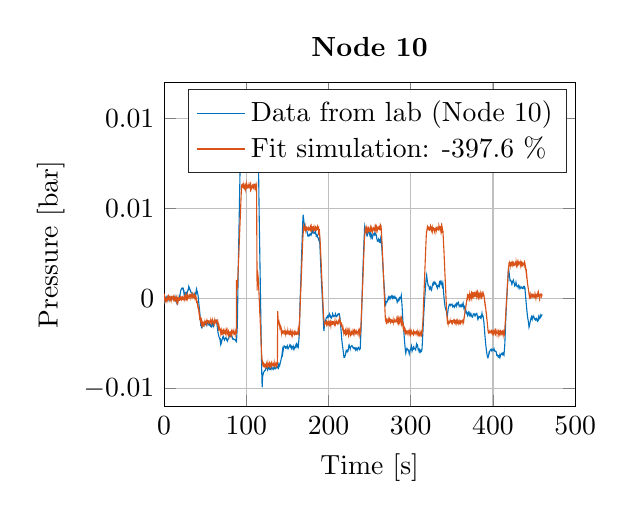
\begin{tikzpicture}

\begin{axis}[%
scaled y ticks = false,
 y tick label style={/pgf/number format/fixed,
/pgf/number format/1000 sep = \thinspace}, % Optional if you want to replace comma as the 1000 separator 
width=2.0556in,
height=1.62135in,
at={(1.011in,0.642in)},
scale only axis,
xmin=0,
xmax=500,
xlabel={Time [s]},
xmajorgrids,
ymin=-0.006,
ymax=0.012,
ylabel={Pressure [bar]},
ymajorgrids,
axis background/.style={fill=white},
title style={font=\bfseries},
title={Node 10},
legend style={legend cell align=left,align=left,draw=white!15!black}
]
\addplot [color=mycolor1,solid]
  table[row sep=crcr]{%
0.05	-0.00026480762463349\\
1.15	-6.73198435972577e-05\\
2.2	7.53585532746459e-05\\
2.4	9.36283479959499e-05\\
2.75	2.75090909090669e-05\\
3.45	4.31689149562875e-05\\
4.1	0.000107548191593421\\
4.3	7.97085043989787e-05\\
4.95	-6.20999022481472e-05\\
5.35	1.0109286412735e-05\\
6.3	9.88482893451159e-05\\
6.45	8.66684261975614e-05\\
7.35	-4.90500488757317e-05\\
7.5	-4.20901270771212e-05\\
8.3	3.70789833821494e-05\\
9.25	-4.81800586516201e-05\\
9.6	2.57691104587898e-05\\
10.15	8.84084066461177e-05\\
10.65	7.70985337233965e-05\\
11.65	-2.81702834803166e-05\\
11.75	-2.29503421313726e-05\\
12.15	1.96791788852901e-05\\
13	2.9249071358789e-05\\
13.7	-6.3839882698008e-05\\
14.3	7.1878592375535e-05\\
14.9	-0.00016475874877761\\
15.25	-0.000143008993157168\\
15.9	-0.000304827174975514\\
15.95	-0.000301347214076153\\
17.05	-0.000109949364614087\\
17.75	1.61992179862069e-05\\
18.1	-8.16050830848569e-06\\
19.15	0.000178017399804442\\
19.35	0.000164967546432304\\
20.2	0.000437274486803918\\
21.25	0.000562553079179018\\
21.9	0.00055124320625638\\
22.25	0.000593002737047932\\
22.95	0.000597352688171154\\
23.4	0.000484253958942998\\
23.65	0.00050078377321483\\
24.25	0.000278066275658767\\
24.55	0.000328525708698346\\
25.15	0.000171927468229138\\
25.5	0.000222386901269439\\
26.05	0.00032852570869818\\
26.85	0.000352015444768566\\
27.5	0.000273716324533962\\
27.7	0.000291116129030738\\
28.7	0.000423354643205698\\
29.75	0.000579952883675267\\
29.95	0.000647812121212149\\
30.4	0.000551243206255853\\
30.8	0.000596482697947293\\
31.85	0.000470334115347526\\
32.95	0.000328525708700317\\
33.95	0.00029807605083032\\
34.05	0.000302426001954265\\
34.85	0.000214556989246162\\
35.25	0.00025544652981313\\
36.1	0.000128427956988281\\
36.6	7.53585532746182e-05\\
37	0.00019889716519958\\
37.15	0.000188457282501692\\
38.2	0.000304165982404098\\
38.7	0.000261536461388351\\
39.3	0.000535583382209798\\
39.5	0.000559943108505295\\
40.25	0.000333745650050038\\
40.55	0.000356365395895675\\
41.4	0.000164967546432554\\
42.45	-0.000337886803518761\\
43.55	-0.000812901466274885\\
44.6	-0.00144886432062627\\
44.9	-0.00143494447702833\\
45.65	-0.00161329247311984\\
45.85	-0.00162286236559278\\
46.55	-0.00152194349951185\\
46.7	-0.00152368347996223\\
47.25	-0.0014314645161311\\
48.45	-0.00150889364614129\\
48.85	-0.00140971476051199\\
49.3	-0.00134620547409903\\
50.1	-0.00141580469208505\\
50.65	-0.00135142541544789\\
50.95	-0.00138709501466563\\
52	-0.00146452414467568\\
52.1	-0.0014723540566986\\
52.9	-0.00133663558162481\\
53.55	-0.00130357595308112\\
54.1	-0.001393184946238\\
54.45	-0.00143494447702991\\
55	-0.00137665513196475\\
55.2	-0.00141145474095722\\
56.25	-0.00151672355816174\\
56.75	-0.00144973431085119\\
57.65	-0.00155848308895506\\
58.35	-0.00149845376344218\\
58.5	-0.00149932375366674\\
59.05	-0.00139492492668786\\
59.9	-0.00152194349951451\\
60.5	-0.00135490537634866\\
61.15	-0.0012304967741982\\
61.75	-0.00129052609971075\\
62.6	-0.00126616637341634\\
63.45	-0.00121396695992779\\
63.65	-0.00125137653959434\\
64.7	-0.00154630322581212\\
65.8	-0.00194301876833436\\
66.85	-0.00212310674487307\\
67.6	-0.00221532570870259\\
67.9	-0.00221445571847731\\
68.7	-0.00248154271749917\\
69.1	-0.0023475642228756\\
69.7	-0.0024484830889562\\
70	-0.00238671378299343\\
71.1	-0.00217704613880756\\
71.35	-0.00220401583577748\\
72.15	-0.00212223675464493\\
72.3	-0.00210744692082293\\
73.2	-0.00226491515151636\\
73.4	-0.00228753489736128\\
73.75	-0.00221532570870012\\
74.45	-0.00222402561094726\\
75.3	-0.00215355640273523\\
76.15	-0.00227622502443617\\
76.4	-0.00226404516128895\\
77	-0.00235017419354649\\
77.45	-0.00228753489735986\\
78.2	-0.00222054565004931\\
78.5	-0.00222315562072517\\
79.55	-0.0020674273704816\\
80.1	-0.00199434819159763\\
80.6	-0.00209874701857651\\
80.65	-0.00209961700880107\\
81.05	-0.00204654760508619\\
82	-0.00203523773216319\\
82.7	-0.00212136676441824\\
82.8	-0.00211527683284374\\
83.7	-0.00224751534701781\\
84.65	-0.00223011554252175\\
84.85	-0.00225621524926603\\
85.2	-0.002282314956011\\
86.7	-0.00226665513196728\\
87	-0.00231276461388205\\
88	-0.00239193372434193\\
88.05	-0.00238671378299274\\
89.1	-0.00150976363636482\\
90.15	0.00148039276637249\\
91.2	0.00409819335288375\\
92.3	0.00684562248289397\\
93.35	0.00953998220918856\\
94	0.0107048991202338\\
94.4	0.0104987114369497\\
95.4	0.0102272744868021\\
95.7	0.0102620740957946\\
96.15	0.0102116146627538\\
97	0.0102533741935461\\
97.6	0.010039356598237\\
98	0.00997932727272585\\
98.4	0.0100828561094798\\
98.65	0.010035006647113\\
99.05	0.00990624809383725\\
100	0.00987666842619611\\
100.4	0.00994017771260908\\
101.5	0.00990450811339236\\
101.75	0.00995409755620721\\
101.95	0.00993843773216205\\
102.2	0.0099941171065496\\
103.1	0.0100036869990227\\
103.75	0.00993321779081463\\
103.95	0.00994800762463732\\
104.7	0.00976965962854245\\
105.05	0.00987144848484939\\
105.65	0.00978966940371259\\
106.5	0.00984969872922511\\
107.1	0.00976356969696546\\
107.5	0.0097687896383136\\
108.15	0.00960871143694397\\
108.55	0.00956608191592714\\
109.25	0.00965482091886052\\
110.3	0.00984273880742356\\
110.45	0.00988188836754211\\
110.9	0.00978879941348518\\
111.4	0.00983229892472942\\
112.35	0.0100410965786893\\
112.4	0.0100297867057663\\
112.75	0.00995061759530749\\
113.65	0.0100376166177896\\
114.55	0.00844118455522896\\
115.6	0.00486639472140532\\
116.65	0.0018666684261931\\
117.7	-0.00109738826979885\\
118.75	-0.00401533548387428\\
119.3	-0.00492360527859498\\
119.85	-0.00433636187683384\\
120.9	-0.00410407448680267\\
121.95	-0.00402490537634101\\
123	-0.0039648760508299\\
123.25	-0.00397009599217946\\
124	-0.00382915757575611\\
124.05	-0.00382915757575611\\
124.95	-0.00376477829911928\\
125.15	-0.00381784770283383\\
126	-0.00396226608015618\\
126.2	-0.00393877634408774\\
127.25	-0.00380740782014038\\
127.65	-0.00379087800587066\\
128.1	-0.00387700703812749\\
128.35	-0.00384568739003435\\
128.85	-0.00389962678397346\\
129.95	-0.00393616637341546\\
130.45	-0.00384307741936063\\
131	-0.0037673882698008\\
131.5	-0.00385438729228363\\
132.55	-0.00392920645161746\\
132.65	-0.00393529638319087\\
133.55	-0.00381697771261494\\
134.25	-0.00378652805474922\\
134.65	-0.00385786725318404\\
134.75	-0.00385438729228504\\
135.1	-0.00389614682307801\\
135.8	-0.00386830713588532\\
136.6	-0.00376129833823094\\
136.9	-0.00381088778104577\\
137.5	-0.00376651827957836\\
137.85	-0.00377173822092652\\
138.9	-0.00388309696970374\\
139	-0.00392311652004615\\
139.55	-0.00362557986315218\\
140.55	-0.00371518885630587\\
141.05	-0.00361166001955049\\
142.1	-0.00342026217008773\\
143.15	-0.00318971476051069\\
144.05	-0.00286259843597131\\
144.4	-0.00300875679374563\\
145.25	-0.0027625495601199\\
145.85	-0.0026242211143731\\
146.45	-0.00262248113392324\\
147.4	-0.00269643030303179\\
147.7	-0.00272513998045193\\
148.1	-0.00266163069403752\\
148.65	-0.0026651106549351\\
149.15	-0.0027155700879731\\
149.9	-0.00261813118279258\\
150.55	-0.00273383988269479\\
150.8	-0.00278255933528648\\
151.65	-0.00270948015639896\\
152.7	-0.00262248113391331\\
153	-0.00257637165199889\\
153.75	-0.0026651106549351\\
154.1	-0.00262335112414286\\
154.8	-0.00274688973606835\\
154.85	-0.00275384965786707\\
155.4	-0.002643360899313\\
156.35	-0.00267468054740611\\
156.7	-0.00274253978494338\\
157.15	-0.00265380078201211\\
158	-0.00281126901270873\\
158.75	-0.00269556031280652\\
159.05	-0.00270078025415749\\
160	-0.00259899139785197\\
160.35	-0.0026668506353878\\
161.15	-0.0024702328445762\\
161.2	-0.0024693628543509\\
162.15	-0.00267468054741393\\
162.2	-0.00267120058651493\\
162.9	-0.002577241642232\\
163.35	-0.00264336089931724\\
164.35	-0.00204393763441141\\
165.4	-0.000209998240475712\\
166.45	0.00116806627565333\\
167.5	0.00268532922775513\\
168.6	0.00417040254153997\\
169.15	0.00465759706744115\\
169.65	0.00445401935483367\\
170.7	0.00405382385141173\\
170.95	0.00397813470185335\\
171.75	0.00399640449657646\\
172.4	0.00390157556206966\\
172.8	0.00391549540566494\\
173.9	0.00368146803519173\\
174	0.00369016793743959\\
174.95	0.00347267038123186\\
175.05	0.003467450439883\\
175.5	0.00351268993157638\\
176.05	0.00349181016617742\\
176.55	0.00355705943304024\\
177.2	0.00351094995112725\\
178.1	0.00359272903225979\\
178.85	0.00363187859237335\\
179.1	0.00356488934506211\\
179.2	0.00357706920820897\\
180	0.00383980625610866\\
180.25	0.0037841268817197\\
181.25	0.0036414484848479\\
181.3	0.00364144848484863\\
181.7	0.00373105747800304\\
182.35	0.00369364789833576\\
182.75	0.00363535855327521\\
183.5	0.0036249186705789\\
184.15	0.00372235757576087\\
184.5	0.00364231847507676\\
185.1	0.00347789032258355\\
186.15	0.00354574956011866\\
186.6	0.00342917086999114\\
187.65	0.00332825200390524\\
188.2	0.00325343284456786\\
188.7	0.0033395618768261\\
189.05	0.00337001153469538\\
189.8	0.00270446901270568\\
190.85	0.00150214252199568\\
191.9	0.000508613685242021\\
192.95	-0.000370946432062813\\
194	-0.00151150361681396\\
194.45	-0.00180208035190851\\
195.1	-0.00143407448680641\\
195.85	-0.00128791612903634\\
196.15	-0.00129574604106034\\
197.2	-0.00106867859237306\\
198.2	-0.00101386920820865\\
198.65	-0.00097906959921723\\
199	-0.00102778905180678\\
199.6	-0.000960799804494816\\
200	-0.00102430909090848\\
200.4	-0.00101560918866064\\
201.25	-0.000852921016618713\\
201.45	-0.000879020723363683\\
202.45	-0.00101908914956034\\
202.75	-0.00098167956988951\\
203.55	-0.00107041857282006\\
204.6	-0.000966019745837265\\
204.95	-0.000839001173012749\\
205.65	-0.000912080351898853\\
206.15	-0.000979069599217924\\
206.75	-0.000950359921806337\\
207.65	-0.00098776950147858\\
207.8	-0.000979939589455997\\
208.4	-0.000839871163262923\\
208.85	-0.000902510459457689\\
209.85	-0.000998209384194759\\
209.9	-0.00099646940374562\\
210.95	-0.000911210361714793\\
211.3	-0.000861620918900657\\
212.05	-0.000881630694067964\\
212.5	-0.000833781231702996\\
213.2	-0.000831171261028552\\
214.15	-0.00115393763442803\\
215.2	-0.00173074115348221\\
216.25	-0.00233451436950455\\
217.35	-0.00272426999022096\\
218.4	-0.00310619569891407\\
218.8	-0.00325148406645676\\
219.65	-0.00324974408601045\\
220.5	-0.00312881544477001\\
221.35	-0.00291218787878827\\
221.7	-0.00295742737048024\\
222.65	-0.00285737849462528\\
222.85	-0.00285389853372559\\
223.45	-0.00293567761485811\\
223.7	-0.00290783792766611\\
224.75	-0.00259290146627428\\
225	-0.00256245180840645\\
225.8	-0.00268425043988069\\
226.4	-0.00279125923752938\\
226.85	-0.00268860039100141\\
227.9	-0.00263292101660889\\
227.95	-0.00263292101660889\\
228.3	-0.00261030127076431\\
229	-0.00262857106548103\\
230	-0.00274862971649903\\
230.2	-0.00275210967739589\\
230.75	-0.0027068701857082\\
231.1	-0.00271209012705848\\
231.75	-0.00277820938414158\\
232.4	-0.00274253978492917\\
233.2	-0.00287042834798037\\
233.25	-0.00286694838708207\\
234	-0.00273731984358314\\
234.6	-0.00274166979470955\\
235.05	-0.00282866881719096\\
235.35	-0.00277994936460352\\
236.4	-0.00272600997066014\\
236.5	-0.00271644007818631\\
237.45	-0.00281822893448755\\
237.75	-0.00283301876830599\\
238.25	-0.00275906959919531\\
238.55	-0.00276428954054275\\
239.6	-0.00167419178884023\\
240.65	-0.000216958162260222\\
241.7	0.00142210342131585\\
242.75	0.00271490889540268\\
243.85	0.003912885434982\\
244.05	0.00401467429128183\\
244.6	0.00384154623653296\\
244.9	0.00385372609968265\\
245.95	0.0036701581622389\\
246.95	0.00347093040074861\\
247	0.00347267038119775\\
248.05	0.003718007624611\\
248.55	0.00382675640271452\\
249.15	0.00370408778101641\\
250.2	0.00353095972627748\\
250.8	0.003627528641237\\
251.25	0.00346571045941965\\
251.4	0.00343091085042538\\
251.95	0.00357097927662345\\
252.55	0.00348572023459121\\
253.2	0.00333434193546445\\
253.35	0.00334739178883944\\
254.35	0.00359794897359159\\
254.45	0.003590989051795\\
255.5	0.00353965962853459\\
255.55	0.00353617966763486\\
256.4	0.00368320801563235\\
256.55	0.00366841818180683\\
257.6	0.00352225982403745\\
258.15	0.00353095972629028\\
258.65	0.00334826177907041\\
259.5	0.00319166353859765\\
260.45	0.00320906334309334\\
260.8	0.00326909266860376\\
260.9	0.00328736246332334\\
261.75	0.00314207409577641\\
261.85	0.0031499040078011\\
262.3	0.00324038299117796\\
262.9	0.00318035366566469\\
263.7	0.00341177106546772\\
263.95	0.00337871143692262\\
265	0.00274448856302961\\
266.1	0.00186579843595716\\
267.15	0.00103060782012185\\
268.2	0.00035723538611529\\
269.25	-0.000343976735090401\\
269.45	-0.000362246529814231\\
270.3	-0.000165628739002638\\
270.95	-0.000176938611931299\\
271.35	-0.00013604907137002\\
271.45	-0.000143878983391882\\
272.45	1.88091886564601e-05\\
272.8	7.62285434938448e-05\\
273.5	-2.99102639437498e-05\\
274.55	0.000114508113383566\\
274.6	0.000117988074281844\\
275.4	2.31591397729103e-05\\
275.6	4.57788856174923e-05\\
276.7	0.000153657673504254\\
276.9	0.000164967546431499\\
277.75	3.70789833802898e-05\\
278.55	0.00013712785924519\\
278.8	0.000124947996092639\\
279.6	2.57691104615654e-05\\
280.6	0.000114508113400608\\
280.9	4.83888563089507e-05\\
281.15	2.83790811388129e-05\\
281.75	6.66586510313649e-05\\
282	6.57886608032565e-05\\
283.05	-8.99395894470578e-05\\
283.55	-0.000197818377332404\\
284.55	-8.21096774294705e-05\\
285.15	-0.000126479178903266\\
285.2	-0.000127349169127128\\
286.2	7.10086021492584e-05\\
286.25	7.18785923745358e-05\\
286.75	-2.29503421329824e-05\\
287.3	2.22891495618438e-05\\
288.35	0.00014147781036164\\
288.5	0.00017453743890819\\
289.4	-0.000364856500484401\\
290.45	-0.00122875679373982\\
291.5	-0.0017742406647151\\
292.6	-0.00243108328445268\\
293.65	-0.002953947409572\\
293.95	-0.00302702658845597\\
294.7	-0.00286520840662724\\
295.3	-0.00275732961875186\\
296.25	-0.00280865904200944\\
296.8	-0.00287216832842099\\
297.35	-0.00285998846527413\\
297.9	-0.00300701681326451\\
298.2	-0.00306965610944937\\
298.95	-0.00291305786898513\\
300	-0.00279473919841203\\
300.85	-0.00263814095795206\\
301.05	-0.00272079002930986\\
301.6	-0.00291044789832917\\
302.1	-0.0028408486803449\\
303	-0.00271209012708121\\
303.5	-0.00276167956989817\\
303.85	-0.00269643030303607\\
304.25	-0.00276080957967573\\
305.3	-0.00279734916911487\\
305.9	-0.00283910869990572\\
306.35	-0.00268338044965966\\
307	-0.00254157204301103\\
307.45	-0.00264597086998386\\
308.2	-0.0025842015640172\\
308.45	-0.00263727096772676\\
309	-0.00283127878785969\\
309.55	-0.00281648895403983\\
310.25	-0.00294089755618848\\
310.75	-0.00283214877808641\\
311.65	-0.00294263753663621\\
311.75	-0.00295046744866093\\
312.4	-0.0028608584555051\\
313.15	-0.00291044789832348\\
313.75	-0.00277298944280269\\
314.85	-0.00181687018571985\\
315.9	-0.000813771456488782\\
316.95	-2.90402736943252e-05\\
318	0.000668691886614503\\
319.05	0.00124810537635447\\
319.35	0.0013168346041163\\
320.15	0.000982758357785302\\
321.2	0.000722631280557884\\
321.55	0.000733071163254162\\
322.25	0.000661731964825024\\
322.65	0.000531233431102229\\
323.95	0.00064346217009692\\
324.35	0.000546893255143094\\
324.6	0.000572122971664951\\
325.3	0.000479904007830434\\
325.45	0.000502523753673573\\
326.45	0.000773960703819715\\
326.7	0.000758300879775992\\
327.5	0.00091489912024309\\
327.55	0.000914029130017785\\
328.1	0.000821810166181852\\
328.7	0.000914899120248752\\
329.6	0.000841819941354849\\
329.85	0.000879229521022123\\
330.65	0.000806150342142403\\
330.75	0.000812240273717957\\
331.6	0.000670431867067917\\
332.3	0.000587782795711506\\
332.8	0.000736551124160989\\
333.35	0.000734811143710407\\
333.9	0.000693051612920992\\
334.65	0.000835730009792063\\
335	0.000739161094835405\\
335.9	0.000968838514190717\\
336.1	0.00095404868036944\\
336.8	0.000854869794735508\\
337.2	0.00091924907137092\\
338.15	0.00074351104595613\\
338.3	0.000703491495614439\\
339.05	0.000870529618777816\\
339.2	0.000818330205290679\\
340.25	0.000173667448692849\\
341.35	-0.000339626783955466\\
342.3	-0.000562344281525573\\
342.5	-0.000559734310846882\\
343.45	-0.000725902443799165\\
344.4	-0.000996469403725719\\
344.5	-0.000986899511251887\\
345.55	-0.000567564222888645\\
346.65	-0.0003596365591583\\
346.85	-0.000373556402755715\\
347.7	-0.0003178770283703\\
347.8	-0.000307437145673994\\
348.6	-0.000378776344113096\\
348.75	-0.000367466471190098\\
349	-0.000333536852422545\\
350.35	-0.00030308719455896\\
350.85	-0.000416185923790308\\
351.05	-0.000442285630533168\\
351.9	-0.000385736265916786\\
351.95	-0.000389216226815065\\
353	-0.000474475268838787\\
353.05	-0.000477955229737065\\
353.7	-0.000360506549382161\\
354.55	-0.000316137047918302\\
355.1	-0.000388346236582682\\
355.3	-0.000418795894454788\\
356.1	-0.000234357966785753\\
356.15	-0.000235227957011058\\
356.65	-0.000316137047919718\\
357.95	-0.000207388269817615\\
358.3	-0.000296127272750996\\
358.9	-0.000424885826028926\\
359.35	-0.000375296383209128\\
360.15	-0.00035702658848244\\
361.05	-0.000447505571860712\\
361.45	-0.000366596480953441\\
361.6	-0.000350936656905471\\
362.05	-0.00041966588466727\\
362.75	-0.000421405865116437\\
363.6	-0.00025436774194168\\
363.7	-0.000240447898342849\\
364.6	-0.000511014858266573\\
364.9	-0.000463165395905851\\
365.45	-0.000511884848500371\\
365.85	-0.000459685434999024\\
366.4	-0.000699802737052058\\
366.9	-0.000619763636364401\\
367.8	-0.000774621896390854\\
368.9	-0.000904250439896892\\
369	-0.000919040273719612\\
369.6	-0.000784191788870375\\
370.3	-0.000744172238528684\\
370.95	-0.000887720625627891\\
371.3	-0.000805071554270065\\
372.05	-0.00090773040080655\\
372.35	-0.000940790029350241\\
373.1	-0.000833781231698721\\
373.15	-0.000826821309900722\\
374.2	-0.000986029521047899\\
374.5	-0.00097297966767862\\
375.1	-0.00102604907139103\\
375.3	-0.00101647917891576\\
376.1	-0.000842481133948719\\
376.55	-0.000846831085070859\\
376.95	-0.000872060801589858\\
377.35	-0.000852921016640723\\
378.2	-0.000966019745866409\\
378.4	-0.000949489931595965\\
378.85	-0.000854660997087031\\
380.15	-0.000883370674505751\\
380.45	-0.000840741153489616\\
380.55	-0.000857270967762891\\
381.6	-0.00115132766375076\\
381.65	-0.00115741759532489\\
382.5	-0.00103213900295096\\
382.65	-0.00105823870969524\\
383.15	-0.00100603929620241\\
383.95	-0.00100603929620668\\
384.7	-0.00105562873901655\\
385.05	-0.001001689345076\\
385.55	-0.00107041857283641\\
385.85	-0.00102256911047285\\
386.65	-0.000811161485847062\\
386.9	-0.000878150733158306\\
387.55	-0.000983419550363546\\
387.95	-0.00097036969699707\\
389	-0.00130879589444879\\
390.1	-0.00197346842620966\\
391.15	-0.00252504222873634\\
392.2	-0.0029252377321462\\
393.25	-0.00322103440857327\\
393.85	-0.0032767137829601\\
394.3	-0.00322625434992638\\
395.2	-0.00301310674484434\\
395.4	-0.00303224652979345\\
396.45	-0.00287129833820424\\
397.15	-0.00282518885628272\\
398	-0.00280169912021003\\
398.55	-0.00288695816224654\\
398.7	-0.00290435796674082\\
399.6	-0.00280865904201227\\
399.65	-0.002807789051787\\
400.65	-0.0028565085043801\\
401.3	-0.00277646940370097\\
401.75	-0.00285824848483351\\
402.3	-0.00291653782990048\\
402.8	-0.00290087800585107\\
403.85	-0.00293480762462003\\
404.6	-0.0031262054740771\\
405.05	-0.00309836578688227\\
406	-0.00318536480936935\\
406.25	-0.00321755444768776\\
406.6	-0.00316013509285035\\
407.4	-0.00316361505374724\\
407.75	-0.00323408426196245\\
408.4	-0.00310706568914221\\
408.9	-0.00319928465296962\\
409.15	-0.00315143519060321\\
410.2	-0.00308444594329621\\
411.05	-0.00302180664709858\\
411.85	-0.00310010576732858\\
412.35	-0.00303224652979203\\
412.4	-0.00302876656889234\\
413.4	-0.00312881544473875\\
414.45	-0.00251112238512186\\
415.5	-0.00121657693058444\\
416.55	-0.00019694838709719\\
417.65	0.000711321407624949\\
418.7	0.00151519237536568\\
419	0.0016935403714563\\
419.75	0.00139600371457013\\
420.8	0.00100624809384661\\
421.45	0.00102538787880285\\
421.85	0.000954918670590471\\
422.45	0.000965358553281059\\
422.95	0.000793100488770265\\
423	0.000787010557196127\\
424	0.000965358553271123\\
424.2	0.000961878592371401\\
424.8	0.00102799784946023\\
425.05	0.000975798435977365\\
426.1	0.000820070185731298\\
426.5	0.000700881524918706\\
427.4	0.00075830087975895\\
428	0.000904459237526883\\
428.25	0.00084703988269233\\
429.05	0.000700881524924396\\
429.3	0.000720021309860708\\
430.35	0.000665211925687775\\
430.6	0.000619102443773362\\
431.3	0.000741771065467217\\
431.4	0.000733071163222909\\
432.45	0.000623452394908325\\
432.65	0.000585172825018604\\
433.1	0.00064694213097391\\
433.55	0.000592132746809498\\
434.6	0.000640852199405434\\
435.5	0.00057212297165074\\
436.25	0.000565163049854156\\
436.65	0.000628672336260017\\
436.85	0.00060866256108702\\
437.45	0.000659991984333252\\
438	0.000593872727243011\\
438.45	0.000646072140731563\\
438.85	0.000611272531745838\\
439.9	2.31591397643893e-05\\
440.95	-0.00050666490716289\\
442	-0.000982549560133994\\
443.05	-0.00126703636364234\\
443.85	-0.00158806275659834\\
444.15	-0.00153934330399955\\
445.2	-0.00129835601171557\\
446.25	-0.00109129833820909\\
446.7	-0.00100690928640781\\
447.7	-0.00115480762463768\\
448.35	-0.00101821915933933\\
448.85	-0.000955579863155892\\
449.45	-0.00102865904204555\\
449.85	-0.00101299921799899\\
450.5	-0.00113044789835534\\
451.05	-0.00112087800588007\\
451.55	-0.00118177732160155\\
451.7	-0.00118699726294472\\
452.25	-0.00111565806448857\\
452.9	-0.00109216832842016\\
453.65	-0.00121048699899043\\
454.15	-0.00125833646134688\\
454.8	-0.0012374566959486\\
455.4	-0.00101995913973588\\
456.05	-0.00112870791783939\\
456.75	-0.00105910869986225\\
456.85	-0.00106345865098867\\
457.55	-0.000920780254133224\\
458.2	-0.00101560918863505\\
458.9	-0.000941660019525808\\
460	-0.000874670772224501\\
};
\addlegendentry{Data from lab (Node 10)};

\addplot [color=mycolor2,solid]
  table[row sep=crcr]{%
0.05	0.000296946837965077\\
1.05	-0.000129763008076037\\
1.15	-9.96730480844371e-05\\
1.3	4.95797311639561e-05\\
2.4	-0.000119265313772599\\
3.2	3.09560392666814e-05\\
3.9	7.85336600890325e-05\\
4	-6.82820685570515e-05\\
4.6	3.9895044482144e-05\\
4.7	-5.20435214705446e-05\\
5.6	-5.19307468523554e-05\\
6	8.98435452445719e-05\\
6.8	-6.80059913847128e-05\\
7.25	0.000120145932253614\\
7.5	-3.1534022383884e-05\\
8.25	7.89300846525903e-05\\
8.7	-6.96918859529436e-05\\
9.1	5.04927844292932e-05\\
9.7	0.000107362640063519\\
10.65	3.39869828075173e-06\\
11.25	-6.38981062515058e-05\\
11.6	6.89872888359638e-05\\
12.3	-3.33448944682528e-05\\
12.5	9.59325535117302e-05\\
13.25	-4.4772687159282e-06\\
13.35	7.94661603814393e-05\\
14	8.03224202890918e-05\\
14.7	-0.000109161989174851\\
15.15	-0.000159805461891921\\
15.4	-2.24127076322241e-05\\
16	-0.000184209065110651\\
16.8	2.61718948661246e-05\\
17.05	-0.000136565266807679\\
17.65	2.2286645705139e-05\\
18.65	4.21293529847306e-05\\
18.85	-8.76802027289153e-05\\
19.55	-8.01156613720915e-05\\
20.15	0.000135945628539889\\
20.2	8.49428177399459e-05\\
21.25	-2.0363315153688e-05\\
21.3	-3.15912294827189e-05\\
22.1	0.000109774892101051\\
22.4	9.61501474162088e-05\\
22.8	-5.04127481417404e-05\\
24.05	-6.77470436287433e-05\\
24.3	8.29741801686587e-05\\
24.65	0.00012771449836355\\
25.3	-5.001699171856e-05\\
26.1	0.000162915041585339\\
26.45	-1.00784295431195e-05\\
27.05	-4.82183280750745e-05\\
27.65	0.000166927900490597\\
27.7	0.000171314592164299\\
28.4	2.08628989481204e-05\\
28.8	0.000186704731153938\\
29.3	4.3081284104012e-05\\
30.4	1.97713092017784e-05\\
30.8	0.000224934256337937\\
31.05	8.17820428986442e-05\\
31.4	0.000239827525658757\\
32.4	0.000238544415441468\\
32.7	4.04368971868969e-05\\
33.7	0.000202933056436604\\
33.8	6.63063528280411e-05\\
34.15	0.000244643169707099\\
34.8	0.000108098934573418\\
35.15	0.000190365021638207\\
35.85	6.27673941464591e-05\\
36.35	5.38154065351069e-05\\
37.05	0.000206634500957919\\
37.15	0.000161094053871036\\
37.6	2.21672063688314e-05\\
38.25	0.00013048731253093\\
39.15	-8.05531843969335e-05\\
39.4	-2.67239740642517e-05\\
40.3	-0.00024982381963426\\
40.4	-0.000143639261730461\\
41.05	-0.000452947602018821\\
41.45	-0.000421004963511\\
42.45	-0.0007853114688459\\
42.7	-0.000725350869514876\\
43.3	-0.00106865963775116\\
43.6	-0.00103084481609644\\
44.55	-0.00126206192842468\\
44.85	-0.00117940395265859\\
45.45	-0.00136375673804409\\
45.8	-0.00125437678114156\\
46.45	-0.00144343801027496\\
46.7	-0.00135603614653573\\
47.25	-0.00146145741564696\\
47.95	-0.00135770782999689\\
48.65	-0.0014737707656919\\
48.95	-0.00143495894608316\\
49.55	-0.00127386408048449\\
49.9	-0.00138188138376444\\
50.95	-0.00127938890650274\\
51.35	-0.00133631744714142\\
51.95	-0.00122796463324026\\
52.05	-0.0013282321926037\\
52.5	-0.00121742858801397\\
53.4	-0.00122865661453321\\
54.05	-0.00135160954907961\\
54.55	-0.00137127913669899\\
54.85	-0.00123485651246005\\
55.55	-0.0012418119490964\\
56	-0.00133497392734577\\
56.35	-0.00132884506987711\\
56.7	-0.0012003128097365\\
57.5	-0.00138240363008296\\
58.1	-0.00124883128316158\\
58.65	-0.00114933745509875\\
59.4	-0.00132417210653853\\
59.55	-0.00122925105868336\\
59.85	-0.00135265649842807\\
60.75	-0.00135295192432509\\
61.1	-0.00122893286553048\\
61.65	-0.00139747096980006\\
62.35	-0.0012424442633663\\
62.75	-0.00127731336740455\\
63.15	-0.00119307962181995\\
64.35	-0.00123561559993149\\
64.55	-0.00137312345331253\\
64.7	-0.00130786450195484\\
65.6	-0.00152688861922926\\
65.8	-0.00139335102444411\\
66.75	-0.00166344308448636\\
67	-0.00156084281604068\\
67.65	-0.0017182463101796\\
68.55	-0.00169657046088608\\
68.95	-0.00189709362743918\\
69.25	-0.00180650374255647\\
69.45	-0.00192328414840319\\
70.1	-0.00197066069405148\\
70.6	-0.00178775375308917\\
71.4	-0.00190866954317568\\
71.75	-0.00179724350671902\\
72.25	-0.0017460485688214\\
72.8	-0.00197338251426451\\
73.2	-0.00177101940209746\\
74.25	-0.00190359861045665\\
74.65	-0.00194183881384477\\
74.9	-0.0017827855829916\\
75.5	-0.00169881601842446\\
76.3	-0.001934893527473\\
76.8	-0.00180367700346592\\
77.1	-0.0019373284214389\\
78.3	-0.00180463182606103\\
78.5	-0.00192189138071056\\
78.65	-0.00202205034921466\\
79.35	-0.00186000309808992\\
80.1	-0.00184740960459852\\
80.5	-0.00201846672429618\\
81.6	-0.00184239519785568\\
81.7	-0.00193192526690755\\
81.8	-0.00196448046458372\\
82.1	-0.00182956960783021\\
82.75	-0.00194716273903378\\
83.65	-0.00178309825537034\\
83.95	-0.0018145167576356\\
84.65	-0.00191321149118844\\
84.95	-0.00181237393840343\\
85.3	-0.00194430750791012\\
86.35	-0.00185526395595075\\
86.6	-0.00198371665199973\\
87.05	-0.00184667385679044\\
87.35	-0.00194870433191838\\
88.1	-0.0019013839141809\\
88.15	0.001030922096788\\
89.1	0.000527126011279466\\
90.15	0.00160315942660757\\
91.2	0.00281858677274673\\
92.3	0.00407756595089839\\
93.35	0.00528445326146519\\
94.25	0.00629864175979277\\
94.7	0.0063271889995587\\
94.9	0.00621165726357577\\
95.8	0.0063027925139161\\
96.4	0.00615556370577428\\
97	0.00613273349629882\\
97.2	0.00633261133956206\\
97.6	0.00626015857340431\\
97.8	0.00613861106642119\\
98.95	0.00629137202275171\\
99.1	0.00612052407229537\\
99.95	0.00634317538616177\\
100.15	0.00611296596711594\\
101.55	0.00616839380718867\\
101.8	0.00629470708101527\\
102.05	0.00633017114797975\\
102.4	0.006153091517811\\
103.15	0.00614812372955191\\
103.7	0.00629483389785887\\
104.35	0.00636244687886913\\
104.95	0.00613618606357154\\
105.45	0.00628572051783207\\
105.7	0.00615392958222221\\
106.1	0.00628098327778274\\
106.3	0.00610331910941945\\
107.45	0.00619927446016246\\
107.75	0.0063192346338928\\
108.25	0.00633708762457487\\
108.65	0.00613813158208126\\
109.4	0.00609840741590147\\
109.75	0.00632479068944027\\
110.7	0.00635890078342701\\
111.1	0.00622086052052545\\
111.35	0.00634205746158216\\
111.65	0.00616173193268345\\
112.45	0.0063062480615385\\
113.15	0.000441712255905482\\
113.65	0.00156531986671603\\
114.55	0.00114990022755799\\
115.6	0.000138312069292668\\
116.55	-0.000936122292185963\\
116.65	-0.000930105272843471\\
117.7	-0.00209239571905256\\
118.75	-0.00320748017057388\\
118.85	-0.00319317839071469\\
119.6	-0.00367654347470479\\
119.85	-0.00356695576816608\\
120.5	-0.0037699189318148\\
121.15	-0.00375186912064847\\
121.3	-0.00364021433370661\\
122.05	-0.00374310722907792\\
122.5	-0.00362825490944438\\
123.2	-0.00363676087858962\\
123.85	-0.00381813393246093\\
124.5	-0.00373999209340778\\
124.65	-0.00361966010226171\\
125.6	-0.00376399847232037\\
126.1	-0.00361283192447369\\
126.3	-0.00375676866596663\\
126.6	-0.00360983328164899\\
127.5	-0.00374321998275041\\
128.3	-0.00358044199297186\\
129	-0.00374314333220999\\
130.05	-0.00359070858293205\\
130.25	-0.00371029374629312\\
130.6	-0.00360191636627717\\
131.1	-0.00371663271958083\\
131.85	-0.00370799138685954\\
132.35	-0.00361678934333936\\
132.55	-0.00365837550764275\\
133.55	-0.00374274159489353\\
133.95	-0.00357956627473701\\
134.35	-0.00373975090656146\\
135.05	-0.00372633972063439\\
135.7	-0.00360541345107391\\
135.8	-0.0035921859244799\\
136.35	-0.00371434821899469\\
137.1	-0.00360394452467195\\
137.35	-0.00371281782753711\\
137.85	-0.00364081755204947\\
138.15	-0.000697394491250998\\
138.9	-0.00125876607263155\\
139.95	-0.00143650909476176\\
140.1	-0.00137960893508886\\
140.75	-0.0015752285232533\\
141.05	-0.00148934869249972\\
142.1	-0.00171593882336243\\
142.65	-0.00185660836905839\\
142.75	-0.00167942766105378\\
143.25	-0.00176323397028719\\
144	-0.00192134247217419\\
144.25	-0.00191839895698502\\
144.4	-0.0017928117815332\\
145.8	-0.00179510385667238\\
146.15	-0.0019596412483169\\
147.05	-0.00194201520987721\\
147.15	-0.00179659250283063\\
147.75	-0.00194570361479358\\
148.05	-0.00180215443146256\\
148.75	-0.00179921207115519\\
149.35	-0.00193332610598259\\
150.1	-0.00188834909150833\\
150.4	-0.00178891769685266\\
150.85	-0.00199011097982263\\
151.15	-0.00182769869682348\\
152.15	-0.00193474054147854\\
152.3	-0.00185287769414707\\
152.75	-0.00182206999791865\\
153.05	-0.00198109921311567\\
154	-0.00198370901121784\\
154.25	-0.00182582198385004\\
155.1	-0.00200796236566672\\
155.8	-0.00185681491365464\\
156.15	-0.00198135117646656\\
156.45	-0.00187855993349501\\
157.3	-0.00193804024758841\\
158	-0.0018403428724521\\
158.7	-0.0019649581697957\\
159.3	-0.0018509224184883\\
159.85	-0.00198293591378712\\
160.75	-0.00198090803641567\\
160.9	-0.00185952650703437\\
161.15	-0.00186345530933321\\
161.3	-0.00197807499233416\\
162.5	-0.00196972483718627\\
163.15	-0.00169111110564354\\
163.95	-0.00192871836483762\\
164.35	-0.00173733739204832\\
165.4	-0.000525647130949595\\
166.35	0.00064696618622184\\
166.45	0.000623551581564169\\
167.5	0.00186215786596139\\
168.6	0.00318653084270672\\
169.65	0.00397234250485307\\
169.75	0.00400629549513137\\
170.3	0.00383592292948718\\
171.15	0.00380064793365775\\
171.75	0.00399175806026246\\
172.15	0.00381920772945556\\
172.8	0.00399366877315629\\
172.85	0.00401543021953598\\
173.2	0.00380320955271724\\
174	0.00382002896921043\\
174.55	0.00391447629148642\\
175.9	0.00381088548893957\\
176	0.00394450414829935\\
176.05	0.00395384790338867\\
176.95	0.00384472970048177\\
177.8	0.00379755828861944\\
178.05	0.00395052230767205\\
178.45	0.00386941690814562\\
179	0.00399637544538148\\
179.45	0.00383306290163027\\
180.2	0.00398178777890813\\
180.9	0.00398781792915063\\
181.3	0.00383322646736039\\
181.45	0.00379115108548912\\
182.35	0.00398763987387627\\
183.05	0.0038002559312149\\
183.7	0.00379773122386722\\
184.3	0.00398028526810378\\
184.85	0.00394244399242576\\
185.2	0.00384542860260215\\
186.45	0.00399775035240098\\
186.55	0.00384454472811636\\
187.1	0.00386674143204481\\
187.6	0.00396935149898722\\
187.85	0.00397978971722172\\
188.15	0.00350931962935197\\
188.75	0.00386967655017532\\
189.8	0.00321310275199261\\
190.85	0.00217269458049252\\
190.9	0.00217334159341446\\
191.9	0.00106089862263298\\
192.95	6.26713612461338e-05\\
194	-0.000970713486021838\\
195	-0.00136520977183532\\
195.15	-0.00131393682472182\\
195.25	-0.00139927704843855\\
197.05	-0.0012825450131395\\
197.15	-0.0014036433115199\\
197.4	-0.00144692359948686\\
198.05	-0.00129730703923869\\
198.55	-0.00142427652622236\\
199.2	-0.00132338928395698\\
199.7	-0.00128443654564313\\
200.2	-0.00143586537888081\\
200.7	-0.00147401581692438\\
201.25	-0.00133124261882316\\
201.75	-0.00141417462814863\\
202.4	-0.00129845375450864\\
202.9	-0.00149254976365268\\
203.3	-0.00133604717671863\\
203.7	-0.00129666566156758\\
203.8	-0.0014286836226459\\
204.65	-0.00142679302313004\\
205.25	-0.00127232352074903\\
205.85	-0.00127379979940888\\
206.25	-0.00141011806168063\\
207.15	-0.00145313622352692\\
207.8	-0.00123867112217879\\
208.15	-0.00147096677609276\\
209.45	-0.00131069044765169\\
209.55	-0.0013997244490152\\
209.95	-0.00126483765816567\\
210.85	-0.00137969151966814\\
211.05	-0.00139512231464487\\
212	-0.00125691282552943\\
212.15	-0.00124043400188377\\
212.75	-0.00136145778225769\\
213.1	-0.00131151014565659\\
213.15	-0.00106233746221284\\
214.3	-0.00124593919400453\\
215	-0.00142568040055851\\
215.2	-0.00137680572158358\\
216.2	-0.00149979754601069\\
216.25	-0.00147955410729168\\
217.35	-0.00170911853222479\\
217.65	-0.00162070262285009\\
218.4	-0.00186027775332852\\
218.6	-0.00177099010343371\\
219.35	-0.00187773080295091\\
220.05	-0.00178858058972143\\
220.3	-0.00196653722027561\\
220.8	-0.00200760030356838\\
221.45	-0.0017570851948373\\
221.55	-0.00178642425304812\\
222.2	-0.0019670187129058\\
223.05	-0.00192950267437382\\
223.35	-0.001794682449069\\
224.2	-0.00199768409974535\\
224.5	-0.00185335798509858\\
224.85	-0.00198074592181798\\
225.75	-0.00177228788262671\\
225.8	-0.00179317890808749\\
226.85	-0.0020196596012214\\
227.9	-0.00185538736955703\\
228.3	-0.00193974164252409\\
228.85	-0.00185798345110998\\
229.55	-0.00193088972053623\\
229.8	-0.00180731509239437\\
230.8	-0.00196158251409408\\
231.05	-0.00185464035913764\\
231.3	-0.00191503546656388\\
231.85	-0.00173315477627639\\
233	-0.00181925161244902\\
233.2	-0.00195096288963524\\
233.7	-0.00193690188559928\\
234	-0.00183374584161829\\
234.75	-0.00194140850097757\\
235.1	-0.00182058738782889\\
236.1	-0.0018154782912589\\
236.2	-0.00191706422051483\\
236.45	-0.00182842941334187\\
236.85	-0.00194831841306288\\
237.65	-0.00178345158196808\\
238.15	-0.00203896347995382\\
238.6	-0.00193383434749329\\
239.6	-0.00138885138308329\\
240.6	-0.000166557970294564\\
240.65	-0.000180898369734495\\
241.7	0.000953433708465662\\
242.75	0.0022155064526711\\
243.8	0.00341329990840633\\
243.85	0.00338769666996189\\
244.75	0.00389319924195501\\
245.65	0.00372945398972886\\
245.95	0.00388421158157184\\
246.35	0.00395840433650711\\
247	0.00377010407170205\\
247.3	0.00371910169643852\\
248.05	0.00388634598443929\\
248.55	0.00380705956174221\\
249.05	0.0039152241406836\\
249.3	0.00387723827891292\\
249.6	0.00373525292141948\\
250.2	0.00376070309757518\\
251	0.00392491573707044\\
251.35	0.0037143016300599\\
252	0.00397027590457141\\
252.5	0.00390192794168635\\
253.35	0.00369559418904061\\
254.45	0.00393224245723751\\
254.5	0.00398860656456052\\
254.9	0.00383667581560719\\
255.95	0.00377974779646636\\
256.4	0.00393439358661176\\
256.7	0.00383146536819442\\
257.4	0.0039967655504551\\
258.05	0.00379761819208068\\
258.55	0.00397785381977873\\
259.5	0.00382276479029411\\
259.65	0.00398378961938604\\
259.8	0.00381391832455235\\
260.05	0.00396884878784512\\
261.3	0.00398883320619131\\
261.5	0.00386426636693473\\
262.05	0.00384352872226575\\
262.3	0.00397182920429647\\
263.1	0.00388348750327393\\
263.15	0.00410354799904383\\
263.95	0.00402429426981087\\
265	0.00316306325192179\\
266.1	0.00205270754556341\\
267.15	0.000965359391691535\\
268.2	-0.000188358661589442\\
269.2	-0.00117424482725937\\
269.5	-0.00121795546828422\\
269.65	-0.00106773485265253\\
270.75	-0.00118768168849058\\
270.95	-0.00129222198813573\\
271.55	-0.00119065190060397\\
272.3	-0.00130401140750835\\
273.2	-0.00114001266794615\\
273.3	-0.0012831297581244\\
273.6	-0.00127065682740536\\
274.2	-0.00112638927340334\\
274.85	-0.00120395950315751\\
275.55	-0.00134353616350048\\
275.6	-0.00133987646752083\\
275.95	-0.00115881563677773\\
277	-0.00119496076875848\\
277.5	-0.00130670344490987\\
278.2	-0.00131054533258158\\
278.6	-0.00118672996817099\\
278.95	-0.00131863489790723\\
279.3	-0.00124990785271123\\
280.45	-0.00128759423147007\\
280.65	-0.00114860297117514\\
280.9	-0.00116126707104403\\
281.45	-0.00128367861677809\\
282.7	-0.00127240796641933\\
283	-0.00114818337748531\\
283.6	-0.00128480873347788\\
284.1	-0.00115349507046616\\
284.15	-0.00112459909632118\\
285.05	-0.00132674953439663\\
285.4	-0.00115117423996671\\
285.85	-0.00126980449003497\\
286.2	-0.00116234821950497\\
286.55	-0.00127910935057599\\
287.7	-0.00108663710792321\\
288.15	-0.00129258975773449\\
288.7	-0.00114474076607243\\
289.1	-0.00136783229822708\\
289.5	-0.00126516255944679\\
290.4	-0.00148148661685326\\
290.45	-0.00145639208141716\\
290.95	-0.00165956532707844\\
291.5	-0.00152388857239857\\
292.5	-0.00176231649668905\\
292.65	-0.00169847019393623\\
293.65	-0.00188388821986322\\
293.75	-0.00180386184496964\\
294.5	-0.00194147580059596\\
295	-0.00189958198763921\\
295.3	-0.0017871521012031\\
296.3	-0.00179848947220282\\
296.45	-0.00192176415511226\\
297.45	-0.00181130625535293\\
297.9	-0.00192056471860165\\
298	-0.00195769041941454\\
298.65	-0.00181406974811356\\
299.35	-0.00194027746205286\\
299.45	-0.00178990114498873\\
300.3	-0.0019670719698004\\
301.05	-0.00181781918454513\\
301.1	-0.00180619395039685\\
301.95	-0.00194897546267751\\
302.8	-0.00197841963352829\\
303.15	-0.00185663932034865\\
303.3	-0.00183358758196629\\
303.6	-0.00199688944523989\\
304.25	-0.00194260588484025\\
304.85	-0.00182192070321858\\
305.4	-0.00183534054451338\\
306.35	-0.0019585359635506\\
306.4	-0.00196752270822923\\
307.05	-0.00183118980851025\\
307.5	-0.00186958648281508\\
308.3	-0.00196956388543604\\
308.55	-0.00186647849838389\\
309	-0.00200166139686972\\
309.65	-0.00189747554386426\\
310.45	-0.00204809437045296\\
311.25	-0.00197216015612273\\
311.4	-0.00186747493456399\\
312.2	-0.0020056571574927\\
312.4	-0.00191492655626316\\
312.9	-0.00184768354942368\\
313.4	-0.00199611631150929\\
313.75	-0.00194718812583539\\
314.85	-0.00120057543000167\\
315.85	3.85852493603825e-05\\
315.9	3.7077151688355e-05\\
316.95	0.00128098959434246\\
318	0.00250511105650661\\
319	0.0036054881885304\\
319.05	0.00360116913828316\\
320.15	0.00395649150703828\\
320.4	0.00399454821290589\\
321	0.00383449225469218\\
321.5	0.00384105376823431\\
321.75	0.00397588653950625\\
322.4	0.0039770934010563\\
322.75	0.00379798770935038\\
323.9	0.00381592943581389\\
324.2	0.00404049460649089\\
324.6	0.00399321905504234\\
325.35	0.00379335998997826\\
326.15	0.003947388301435\\
326.45	0.00380082868732169\\
326.55	0.00383911697081936\\
327	0.00393965950072777\\
327.85	0.00393579617383455\\
328.25	0.00379879126641491\\
329.25	0.00367159834507218\\
329.4	0.0039167128097499\\
329.65	0.00377314959214334\\
330.65	0.00391441721782503\\
331.15	0.00380468729704833\\
331.4	0.00391340374752699\\
332.15	0.00395410480747468\\
332.45	0.0038255620599915\\
333.65	0.00381050404622463\\
333.85	0.00393582234737613\\
334	0.00384441002196452\\
334.2	0.00405660549342761\\
335.45	0.00384886315123427\\
335.8	0.00399839935248485\\
336.55	0.0040029590586044\\
336.75	0.00384465747035703\\
337.25	0.00399582201245002\\
337.7	0.00379220846557522\\
338.15	0.00397971784082002\\
339.15	0.00372404229731747\\
339.2	0.00374964320002192\\
340.25	0.00277138757187643\\
340.3	0.00279283224313199\\
341.35	0.00161346010021517\\
342.4	0.000599621018455183\\
343.45	-0.000543357194220626\\
344.5	-0.00124146602335881\\
344.9	-0.00115322393443362\\
345.55	-0.00135574674184396\\
345.85	-0.00123190200291383\\
346.1	-0.00138585416974978\\
347.05	-0.00135499252387038\\
347.7	-0.00123920138393015\\
347.8	-0.00134888243203751\\
348.3	-0.0012021555033866\\
349.55	-0.00120658446530905\\
349.7	-0.00134790680950016\\
349.9	-0.00136045823602087\\
350.5	-0.00123505736969786\\
351.1	-0.00122104543553882\\
351.2	-0.00132286176247407\\
352.3	-0.00119427036553364\\
353	-0.0013075448634631\\
353.3	-0.00133591117567879\\
353.7	-0.00119320522169741\\
354.2	-0.00121255986931609\\
354.3	-0.00135234635093161\\
355.4	-0.00122188464359783\\
356	-0.00136959063524247\\
356.6	-0.00124250145662876\\
356.95	-0.00136538557417228\\
357.3	-0.0013559181635922\\
358.3	-0.00123304093791714\\
358.55	-0.00121620451352201\\
358.7	-0.00140727506576497\\
359.5	-0.00135689739035572\\
360.25	-0.00122360349806066\\
360.7	-0.001247921748248\\
360.8	-0.00136564397010626\\
361.85	-0.00129200015782641\\
362.35	-0.00120037487040183\\
362.9	-0.00119263387262807\\
363.6	-0.00135828893606212\\
364.5	-0.00114515651586276\\
364.65	-0.00118659952357815\\
365.65	-0.000855145163194552\\
365.7	-0.000874709646329133\\
366.25	-0.00055073670866739\\
366.75	-0.000560888263752226\\
367.8	-0.000202347764202469\\
368.9	0.000133368239233683\\
369.1	9.94197191957858e-05\\
369.35	0.000233493809231353\\
370.45	0.000203934417049259\\
370.85	4.39861166693597e-05\\
371.45	0.000213698650369198\\
371.65	5.71434281422348e-05\\
372.25	0.00021494070999293\\
373.1	9.53384510422764e-05\\
373.15	7.71447908067065e-05\\
373.75	0.000252090618656029\\
374.3	6.52280885195581e-05\\
374.7	0.000261226101110473\\
375.5	0.000131724713675185\\
375.85	0.000334461511694858\\
376.65	0.000319726431027869\\
377.1	0.000163761617038332\\
377.8	0.000287180839243107\\
378.35	0.000126757779274622\\
378.45	0.000126720539826717\\
379.35	0.000312859705227403\\
380.1	0.00013740588165451\\
380.45	0.000283189623857089\\
380.65	0.000342568681825004\\
381.25	0.000198244448118081\\
381.8	9.35845555535462e-05\\
381.95	0.000281027451772161\\
382.85	0.000109957621610475\\
383.35	0.000300224980979712\\
384.1	0.000256230146872546\\
384.4	0.00013209655064266\\
385.1	0.000308712675601113\\
385.65	0.000128093410885162\\
386.05	6.88168387326101e-05\\
386.7	0.000233537435953074\\
386.95	0.000136624329560472\\
387.9	0.000273999888181249\\
388.1	0.000108938473333307\\
388.35	0.000283879995583847\\
389	0.000205931473563446\\
390.05	-0.000208722674460501\\
390.15	-0.000173486356714258\\
391.15	-0.000518204917610366\\
392.1	-0.000940353004073226\\
392.2	-0.000917265587451568\\
393.25	-0.00140813692356328\\
394.2	-0.00185049745182464\\
394.3	-0.00175968108513064\\
394.65	-0.00191098624310272\\
395.85	-0.00189101476150218\\
396.25	-0.00177953846026097\\
396.85	-0.0018224698061565\\
397.25	-0.00189757950684014\\
397.6	-0.0018972691599807\\
398.2	-0.00179987112262888\\
398.9	-0.0019142004838846\\
399.2	-0.00179333270713333\\
399.75	-0.0017733155732314\\
400.3	-0.00190879261102389\\
401.05	-0.00181138598306271\\
401.15	-0.00194313863518775\\
402.25	-0.00182713091307473\\
402.7	-0.00191189495669666\\
402.95	-0.00181343658282111\\
403.65	-0.00195037269532654\\
403.95	-0.0017971223858568\\
404.7	-0.00191963138275861\\
405.75	-0.00188876259845551\\
405.95	-0.00182618528404774\\
406.15	-0.00186520274821919\\
406.35	-0.00200979610610283\\
407.1	-0.00182447852621752\\
408.1	-0.00198505231239446\\
408.65	-0.00181607727821518\\
409.2	-0.00192115805413803\\
409.7	-0.00183037921660116\\
410.65	-0.00195618331160643\\
411.25	-0.00180073551814077\\
411.5	-0.00179200318543846\\
412.3	-0.00199603847793533\\
412.35	-0.00195642518042737\\
413.1	-0.00181415391830932\\
413.85	-0.00196386398732309\\
414.45	-0.00168637793045828\\
415.5	-0.00091500039077012\\
416.55	-0.000103940029042124\\
417.65	0.00078648472653026\\
418.7	0.00157260259679913\\
419.65	0.00199906938545836\\
419.95	0.00203119448374317\\
420.65	0.00190599216834295\\
421	0.00183268423735902\\
421.15	0.00199720687310788\\
422.3	0.00201873117528388\\
422.65	0.00184817538633053\\
423.25	0.00181388384511222\\
423.6	0.00201827309708386\\
424.6	0.00190824298946343\\
425	0.00199309578929533\\
425.05	0.00198742472030451\\
425.55	0.00183531833279089\\
426.1	0.00185410978611274\\
427.15	0.00198991179288797\\
428.05	0.00187512043911547\\
428.25	0.00203560480005902\\
428.95	0.00183844991605265\\
429.55	0.00196549391915933\\
429.65	0.00186771618363894\\
430.55	0.00201719992394505\\
430.8	0.00188784757317474\\
431.45	0.00192229578323101\\
432	0.00204264257055908\\
432.85	0.00204159777515493\\
433.3	0.00185053946050887\\
433.95	0.00202885513108907\\
434.55	0.00191649544411534\\
434.65	0.00199772651789912\\
435.65	0.00188717004638549\\
435.75	0.00199092908860385\\
437.55	0.00187458722326313\\
437.65	0.0020161332394384\\
437.95	0.00189304921811299\\
438.4	0.00203720616156625\\
438.85	0.00197983763406901\\
439.9	0.00163170296054838\\
440	0.00164307103404768\\
440.75	0.00133037690165973\\
440.95	0.00139028983737572\\
442	0.000862909233659824\\
443.05	0.0005339401563173\\
444.15	0.000155893683004056\\
444.45	0.000200368721398316\\
444.7	0.000116555096834525\\
445.25	0.000221608861803037\\
445.55	3.02792735202315e-05\\
446.25	5.30306569621162e-05\\
447	0.000238599757526508\\
447.45	0.00022052985460631\\
447.85	0.000116429333612703\\
448.4	8.7572387055391e-05\\
448.85	0.000235875827507294\\
449.55	0.000189262103545251\\
450.3	7.67879066236907e-05\\
450.7	0.000103126020286718\\
451.15	0.000268224498368706\\
451.95	7.41075046551189e-05\\
452.05	0.000203775045058728\\
453	0.000230348920373511\\
453.5	0.000103589890842388\\
454.25	0.000245690555685794\\
454.55	0.00012865561106395\\
455.4	0.000145845752156191\\
455.55	0.000286230523423863\\
456.35	7.73696023478031e-05\\
456.5	0.000251869449092022\\
457	0.000110556463698207\\
457.25	0.000234915967762866\\
458.5	0.000269792298168375\\
458.95	0.000115678046716382\\
460	0.000229881937745764\\
};
\addlegendentry{Fit simulation: -397.6 \%};

\end{axis}
\end{tikzpicture}% 
    \caption{Estimation comparison for node 10.}
  \end{minipage}
  \hfill
  \begin{minipage}[b]{0.45\textwidth}
    % This file was created by matlab2tikz.
%
%The latest updates can be retrieved from
%  http://www.mathworks.com/matlabcentral/fileexchange/22022-matlab2tikz-matlab2tikz
%where you can also make suggestions and rate matlab2tikz.
%
\definecolor{mycolor1}{rgb}{0.00000,0.44700,0.74100}%
\definecolor{mycolor2}{rgb}{0.85000,0.32500,0.09800}%
%
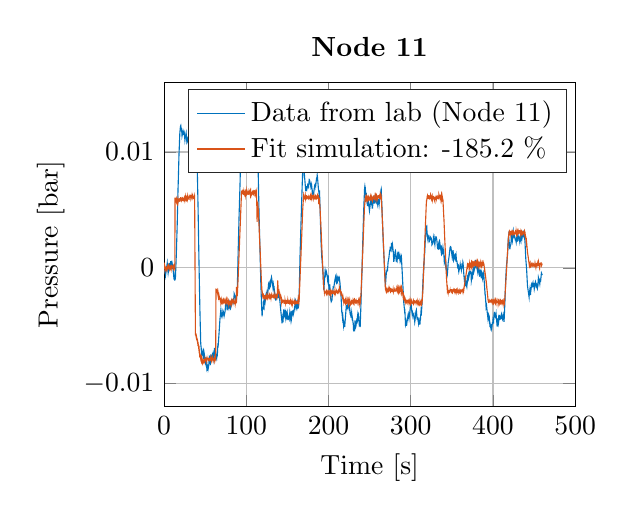
\begin{tikzpicture}

\begin{axis}[%
scaled y ticks = false,
 y tick label style={/pgf/number format/fixed,
/pgf/number format/1000 sep = \thinspace}, % Optional if you want to replace comma as the 1000 separator 
width=2.0556in,
height=1.62135in,
at={(1.011in,0.642in)},
scale only axis,
xmin=0,
xmax=500,
xlabel={Time [s]},
xmajorgrids,
ymin=-0.006,
ymax=0.008,
ylabel={Pressure [bar]},
ymajorgrids,
axis background/.style={fill=white},
title style={font=\bfseries},
title={Node 11},
legend style={legend cell align=left,align=left,draw=white!15!black}
]
\addplot [color=mycolor1,solid]
  table[row sep=crcr]{%
0.05	-8.01913489730799e-05\\
1.1	-0.000215039833821623\\
1.35	-0.000128910801563603\\
1.8	-0.000318568670576308\\
2.2	-0.000214169843596734\\
3.25	4.59572336267422e-05\\
3.85	0.000204295454545617\\
4.3	9.41764418396773e-06\\
4.95	-0.000228959677419427\\
5.5	-0.000100201124144939\\
6.1	0.000189505620723313\\
7	0.000192115591397535\\
7.25	2.94274193544941e-05\\
7.5	6.77069892467685e-05\\
8.15	0.000282594574779471\\
8.8	1.63775659819121e-05\\
9.45	0.000302604349950775\\
9.6	0.000230395161289948\\
10.65	4.59572336265202e-05\\
11.75	-0.000356848240469138\\
12.2	-0.000291598973606755\\
12.75	-0.000526496334310317\\
13.45	-0.000522146383185762\\
13.8	-0.000367288123166304\\
13.85	-0.000404697702833939\\
14.9	0.000576651270772943\\
15.95	0.0018216072825028\\
17	0.00343804912023474\\
17.05	0.00343804912023474\\
18.1	0.00483525342131003\\
19.15	0.00580442253176891\\
19.9	0.0060993492179858\\
20.35	0.00613936876832794\\
21.05	0.00592448118279595\\
21.25	0.00602801001955061\\
21.85	0.00569045381231717\\
22.95	0.00587228176930757\\
23.25	0.00576179301075438\\
23.75	0.00577310288367738\\
24.4	0.00586619183773468\\
24.45	0.00585923191593599\\
25.35	0.0055086258553301\\
25.55	0.00556082526881974\\
26.4	0.005746133186708\\
26.85	0.00582356231671732\\
27.65	0.00545729643206436\\
27.7	0.00543728665689316\\
28.7	0.0055669152003919\\
29.4	0.00541901686217039\\
29.8	0.0055068858748776\\
30.55	0.00584705205278557\\
30.8	0.00580181256109413\\
31.55	0.00596015078201265\\
32.3	0.00603496994134772\\
32.95	0.0058792416911031\\
33.15	0.00582530229716363\\
34	0.00596276075268656\\
34.3	0.00600191031280387\\
34.95	0.00586967179863032\\
35.7	0.00602453005865036\\
35.9	0.00588011168132874\\
36.9	0.00579833260019583\\
37.15	0.00604105987292258\\
37.75	0.00628465713587531\\
39	0.00630553690127145\\
39.3	0.00620983797653987\\
40.35	0.0043437089442824\\
41.4	0.00249845967741966\\
42.45	0.000264324780058306\\
43.55	-0.00176710239491712\\
44.6	-0.00330959506353792\\
44.7	-0.00328697531769248\\
45.65	-0.00373154032258058\\
45.75	-0.00379069965786891\\
46.25	-0.00361235166177862\\
47.25	-0.00378286974584438\\
47.65	-0.00367412096773997\\
48.35	-0.00393946798631303\\
48.7	-0.00367325097751522\\
48.85	-0.00370457062560922\\
49.9	-0.00396730767350895\\
50.25	-0.00406300659824033\\
50.7	-0.00390553836754637\\
51.1	-0.0039185882209187\\
51.95	-0.00431791373411536\\
52.25	-0.00425266446725323\\
52.65	-0.00444667228738971\\
53.4	-0.00417175537634404\\
53.7	-0.00435010337243411\\
54.25	-0.00424831451612931\\
55.15	-0.00382288929618801\\
55.4	-0.0038315891984366\\
56.25	-0.0041604455034237\\
56.3	-0.00416218548387357\\
56.9	-0.00385246896383484\\
57.3	-0.00389683846530153\\
57.5	-0.00382375928641684\\
58.75	-0.00372980034213641\\
59.2	-0.00393163807429581\\
59.65	-0.00377155987292829\\
60.4	-0.00394642790811922\\
60.5	-0.00387943866080762\\
61.3	-0.00345575342131474\\
61.55	-0.0035540623167202\\
62.2	-0.0037732998533771\\
62.65	-0.00367325097752144\\
63.3	-0.00383071920821484\\
63.95	-0.00391597825024639\\
64.45	-0.00371240053763677\\
64.7	-0.00382288929618943\\
65.4	-0.0033356947702847\\
65.8	-0.00335918450635561\\
66.85	-0.00283110043988422\\
67.9	-0.00225081695992466\\
68.95	-0.00184714149560514\\
69.1	-0.00180451197458864\\
69.95	-0.00208812878788414\\
70.35	-0.00213075830890097\\
71	-0.00200373973607362\\
71.15	-0.00208725879765673\\
71.65	-0.00185149144672833\\
72.45	-0.0019254406158383\\
73.05	-0.00207420894428387\\
73.2	-0.00204462927664059\\
74.25	-0.00188281109482183\\
74.9	-0.00151654521016922\\
75.65	-0.00153046505376664\\
76.35	-0.00167140347018679\\
76.7	-0.00183496163245542\\
77.25	-0.0016244239980471\\
78.15	-0.00156439467253455\\
78.5	-0.00172795283480176\\
78.7	-0.00175318255132148\\
79.5	-0.00153220503421367\\
79.55	-0.00154438489736086\\
80.6	-0.00176101246334334\\
80.75	-0.00177145234604104\\
81.7	-0.00161659408602169\\
82.05	-0.00140431647116387\\
82.9	-0.00138343670576774\\
83.8	-0.00151306524926739\\
83.85	-0.00152263514174086\\
84.65	-0.00134689711632574\\
84.85	-0.00138082673509402\\
85.25	-0.00111373973607073\\
86.3	-0.00121204863147795\\
87	-0.00138256671554388\\
87.05	-0.00140344648094001\\
87.35	-0.00128599780058899\\
88.05	-0.00135559701857502\\
89.1	-0.000832732893452842\\
90.15	0.000754129276633236\\
91.2	0.00221223289344954\\
92.3	0.00351199828934398\\
93.35	0.00499533162267718\\
94.05	0.00584879203323418\\
94.4	0.00553733553274563\\
95.4	0.00530417815249379\\
95.8	0.0052980882209186\\
96.5	0.00543728665689103\\
96.6	0.00538508724340139\\
97.05	0.00567131402736989\\
97.6	0.00564260434994907\\
98.65	0.00537725733137598\\
99.1	0.00533462781036056\\
99.4	0.00549731598240391\\
100.25	0.0054007470674462\\
100.75	0.00561998460410237\\
101.8	0.00533984775170801\\
102.8	0.00515975977517072\\
102.9	0.00522587903225741\\
103.9	0.00486744305962739\\
104.3	0.00478740395894187\\
105	0.00495531207233404\\
105.15	0.00500403152492468\\
105.5	0.00478392399804428\\
106.85	0.00502665127077137\\
107.1	0.00481785361681325\\
107.9	0.00476217424242323\\
108.15	0.0048891928152488\\
108.9	0.0051519298631478\\
109.25	0.00512409017595153\\
110.3	0.00531374804496018\\
110.5	0.00541466691103792\\
111.05	0.00523544892472202\\
111.65	0.00532853787877932\\
112.15	0.00558518499510349\\
113	0.00559388489735135\\
113.4	0.00532766788855227\\
113.45	0.00532766788855227\\
114.55	0.00400267277614488\\
115.6	0.00220875293255021\\
116.65	0.000784578934506758\\
117.7	-0.000702234359729353\\
118.75	-0.00176884237537053\\
119.25	-0.0020985686705822\\
119.8	-0.00172186290323226\\
120.65	-0.00175144257087764\\
120.9	-0.00154438489736905\\
121.65	-0.00167488343109468\\
121.9	-0.00148870552298005\\
122	-0.00150958528837478\\
122.7	-0.00134254716520574\\
123	-0.00144694599218567\\
123.9	-0.00121030865103378\\
124.05	-0.00125032820137619\\
125	-0.00106850024438657\\
125.4	-0.00119464882698436\\
126.2	-0.00106502028348046\\
127.15	-0.000670044721408081\\
127.5	-0.000642205034213944\\
128.2	-0.000885802297165256\\
128.3	-0.000879712365591118\\
129.2	-0.000640465053759115\\
129.6	-0.000706584310845804\\
130.4	-0.00044645723362266\\
130.65	-0.000405567693056386\\
131.5	-0.000602185483872253\\
132.5	-0.000875362414468978\\
132.95	-0.000724854105573186\\
133.6	-0.000885802297168115\\
133.85	-0.000869272482895561\\
134.6	-0.00113374951124653\\
134.7	-0.0011024298631527\\
135.75	-0.00137125684262371\\
135.8	-0.00141649633431426\\
136.8	-0.0011798589931567\\
137.6	-0.00114157942326484\\
137.75	-0.00123292839687408\\
137.85	-0.00121639858260295\\
138.25	-0.000957141495604358\\
139.3	-0.00130513758553491\\
139.6	-0.00113113954056857\\
140	-0.00118855889540598\\
141.05	-0.00150871529814595\\
142.1	-0.0019054308406696\\
143.15	-0.00225081695992499\\
143.4	-0.00239871529814564\\
144.1	-0.00218469770283833\\
144.6	-0.00235521578690495\\
145.25	-0.00198894990225199\\
145.45	-0.00179494208211195\\
146.35	-0.00207159897360554\\
146.6	-0.0020924787390024\\
147.15	-0.00192805058650988\\
147.85	-0.0021324982893455\\
148.35	-0.00191065078201133\\
148.9	-0.00195415029325416\\
149.15	-0.0020724689638294\\
149.75	-0.00194023044965461\\
150.55	-0.00225255694037271\\
151	-0.00210030865103136\\
152.2	-0.00222210728250347\\
152.6	-0.00208464882697981\\
152.95	-0.00192283064516105\\
153.75	-0.0021472881231675\\
154.15	-0.00206028910068398\\
154.55	-0.00229605645161199\\
154.8	-0.00224907697947302\\
155.7	-0.00186454130009481\\
155.95	-0.00198024999999488\\
156.75	-0.00185149144671912\\
157.2	-0.00184453152492112\\
157.35	-0.00198372996089319\\
158	-0.00188803103616322\\
158.85	-0.00168967326490319\\
159.05	-0.00169141324535232\\
159.5	-0.00137647678396619\\
160.1	-0.00143215615835587\\
160.6	-0.00170011314760443\\
161.35	-0.0015539547898365\\
161.75	-0.00168880327468499\\
162.45	-0.00151915518084153\\
163.15	-0.00172708284457543\\
163.3	-0.00172099291300057\\
164.35	-0.00107807013685401\\
165.4	0.000568821358748167\\
166.45	0.00182769721407597\\
167.5	0.00302567375366239\\
168.6	0.00422800024437806\\
168.95	0.0046012260508283\\
169.65	0.00438111852394826\\
170.55	0.00398179301075302\\
170.7	0.00400789271749943\\
171.7	0.00357028763441022\\
171.75	0.00357028763441022\\
172.25	0.00333104032258391\\
173.25	0.00333800024438405\\
173.55	0.00352069819159539\\
173.9	0.00343369916911399\\
174.7	0.00357550757576122\\
175.7	0.00349024853372826\\
176	0.00362248704790305\\
176.55	0.00380344501466526\\
177.05	0.00377473533724795\\
178.1	0.00358855742913122\\
178.55	0.00348502859237584\\
179.35	0.00359899731182892\\
180.2	0.00330320063538622\\
180.35	0.0033119005376355\\
181.25	0.00308048313783105\\
181.3	0.00308918304008032\\
182.3	0.00333539027370391\\
182.35	0.00332321041055636\\
183.2	0.00357028763440881\\
184	0.00355984775171322\\
184.2	0.0036668565493676\\
184.5	0.00356767766373722\\
185.55	0.0038947939882695\\
185.75	0.00381127492668426\\
186.25	0.00399745283479747\\
186.6	0.00390262390028853\\
187.65	0.0034458790322516\\
188.6	0.00317183211143315\\
189	0.00334409017594681\\
189.8	0.00250715957966308\\
190.85	0.00115258479961028\\
191.9	0.000388733382210515\\
192	0.000436582844576205\\
192.95	-9.32412023453844e-05\\
193.05	-7.41014174005239e-05\\
194	-0.000751823802541324\\
194.35	-0.000978891251221498\\
195.1	-0.000513446480939594\\
195.95	-0.000128910801565629\\
196.2	-0.000186330156403763\\
196.5	-0.000292468963832143\\
197.35	-0.00016371041055635\\
198.2	-0.000310738758550283\\
198.25	-0.000287249022480424\\
198.9	-0.000522146383183181\\
199.65	-0.000328138563045283\\
200.4	-0.000829252932551011\\
200.7	-0.000962361436947529\\
201.45	-0.000735293988270186\\
201.5	-0.000718764173998354\\
202.5	-0.00130600757575947\\
203.3	-0.0014626058162294\\
204.15	-0.00140605645161584\\
204.6	-0.00121987854350267\\
204.65	-0.0012364083577738\\
205.65	-0.000831862903225428\\
206.35	-0.000845782746822871\\
206.75	-0.00077009359726446\\
207.8	-0.000515186461388012\\
208.35	-0.000427317448679937\\
208.85	-0.000592615591395562\\
209.1	-0.000487346774191766\\
209.9	-0.000710064271749078\\
210.35	-0.000426447458456075\\
211	-0.000559555962854008\\
211.65	-0.000430797409578215\\
212.5	-0.000514316471159182\\
213.05	-0.000409917644181385\\
213.1	-0.00041426759530494\\
214.1	-0.000759653714563185\\
214.15	-0.000749213831865492\\
215.2	-0.00120160874877598\\
216.2	-0.00194284042033119\\
216.3	-0.00190978079178747\\
217.1	-0.00219426759530933\\
217.45	-0.00210987854349881\\
218.35	-0.00249963416422516\\
218.8	-0.00237522556207437\\
219.45	-0.00248049437927605\\
219.65	-0.00255879349951171\\
220.5	-0.00216990786901561\\
221.55	-0.00168793328446043\\
221.75	-0.00160963416422474\\
222.2	-0.00176362243401812\\
222.65	-0.00175405254154357\\
223.3	-0.00162442399804105\\
223.7	-0.00172360288367429\\
224.6	-0.00150958528836839\\
224.8	-0.00150262536656967\\
225.75	-0.00181408186705467\\
225.85	-0.00178189222873626\\
226.85	-0.00203766935483585\\
227.15	-0.00203331940371371\\
227.35	-0.00214554814271622\\
228.1	-0.00193936045943716\\
228.85	-0.00227256671554357\\
229.05	-0.00216729789834189\\
230	-0.00240219525903612\\
230.05	-0.00239001539588998\\
230.5	-0.00272409164222451\\
231.65	-0.00271887170087423\\
232.1	-0.00235782575756802\\
232.3	-0.00227517668621088\\
233.05	-0.00255705351905405\\
233.3	-0.00253182380253505\\
234.3	-0.00226647678397654\\
234.9	-0.00231867619746651\\
235.15	-0.00212901832845289\\
235.5	-0.00203766935484792\\
235.85	-0.0021829577223906\\
236.6	-0.00206202908114733\\
237.45	-0.00247527443794213\\
238.2	-0.00243090493647116\\
238.45	-0.00255531353862123\\
238.55	-0.00252399389052668\\
239.6	-0.00141040640273588\\
240.6	-0.00023765957966701\\
240.65	-0.00023765957966701\\
241.7	0.0011708545943398\\
242.75	0.00244713025416046\\
243.85	0.00341455938416488\\
244.2	0.00350938831866812\\
244.85	0.0033032006353855\\
244.95	0.00331973044965736\\
245.25	0.00316835215053629\\
245.95	0.00319184188660188\\
247	0.00281252614857749\\
247.4	0.00266636779080529\\
248.05	0.00289256524925377\\
248.5	0.00292823484846907\\
249.15	0.00266984775169504\\
249.8	0.00246540004885731\\
250.2	0.00258197873898269\\
251.25	0.00287255547407228\\
251.4	0.00285167570867401\\
251.85	0.0029995740468968\\
252.4	0.00294215469206363\\
253.15	0.00258197873899549\\
253.55	0.00258110874877163\\
254.3	0.00297173435972611\\
254.6	0.00294476466275798\\
255.5	0.00284210581622574\\
255.7	0.00276815664711508\\
256.5	0.00309005303031343\\
256.65	0.00308222311829012\\
257.6	0.00282818597262691\\
257.85	0.0028073062072258\\
258.55	0.00296129447701701\\
258.95	0.00293084481914777\\
259.65	0.00276467668619973\\
259.7	0.00278642644181901\\
260.15	0.00296651441835735\\
260.8	0.00294476466273666\\
261.5	0.00271769721404866\\
261.85	0.00282992595305331\\
262.9	0.00307874315736342\\
263.9	0.00336844990223484\\
264.1	0.00339628958943108\\
265	0.00260024853371646\\
266.1	0.00153190053762473\\
267.15	0.000662780303023275\\
268.2	9.4176441783056e-06\\
269.2	-0.000742253910071045\\
269.3	-0.000734423998046324\\
270.3	-0.000229829667659359\\
271.4	-6.4531524935213e-05\\
271.65	-0.000151530547420869\\
272.45	0.000235615102623959\\
273.5	0.00045311265884096\\
274.4	0.000755869257075964\\
274.55	0.000688010019542273\\
275	0.00084286827956162\\
276.05	0.000758479227753239\\
276.6	0.00105514589441696\\
276.8	0.00105601588464369\\
277.65	0.000876797898327758\\
277.9	0.000960316959908031\\
278.8	0.000671480205267583\\
279.4	0.000253014907135307\\
279.85	0.000382643450632825\\
280.9	0.000668000244377825\\
281.1	0.000696709921795102\\
281.8	0.000480082355817618\\
282	0.000555771505376029\\
282.85	0.000287814516130996\\
283.3	0.000263454789831613\\
284.1	0.00056795136851151\\
284.4	0.000698449902232889\\
284.95	0.000405263196464611\\
285.7	0.000394823313765474\\
286	0.000568821358733956\\
286.25	0.000527931818168376\\
287.15	0.000252144916892988\\
287.3	0.000267804740939542\\
288.3	0.000547941593341372\\
288.55	0.000523581867049067\\
289.4	-4.27817693116617e-05\\
289.45	-4.10417888625225e-05\\
290.45	-0.000784013440861875\\
290.5	-0.000780533479963597\\
291.5	-0.00148522556207326\\
292.6	-0.00188629105572261\\
292.9	-0.00186367130987947\\
293.65	-0.00246918450636088\\
294.7	-0.00233520601173409\\
294.95	-0.00250137414467361\\
295.7	-0.00225168695014388\\
295.8	-0.00226125684261774\\
296.75	-0.00202983944281185\\
297	-0.00199068988269402\\
297.9	-0.00220470747800136\\
298.95	-0.0018810711143695\\
299.95	-0.00153220503421722\\
300.35	-0.00151741520039878\\
301.05	-0.00181669183773692\\
301.85	-0.00203853934506468\\
302.25	-0.00192718059628674\\
303.2	-0.00204723924731895\\
303.75	-0.0020098296676474\\
304.1	-0.00222210728250985\\
304.3	-0.00212379838710688\\
304.9	-0.00233781598241278\\
305.3	-0.00224211705767999\\
306.35	-0.00187411119257574\\
306.85	-0.00181930180841419\\
307.4	-0.00204984921799478\\
307.75	-0.00219687756598802\\
308.5	-0.00217338782992102\\
309.55	-0.00241611510263709\\
309.9	-0.00232737609970654\\
310.2	-0.00243525488758478\\
311.2	-0.00243090493646406\\
311.6	-0.00219861754644143\\
311.85	-0.00221079740958971\\
312.55	-0.00184888147605819\\
313.05	-0.00191674071359899\\
313.7	-0.00156874462366915\\
313.75	-0.00158092448681599\\
314.85	-0.0005786957478216\\
315.7	3.72573313603686e-05\\
315.9	-3.63220920518437e-06\\
316.8	0.000618410801550923\\
316.95	0.000613190860203477\\
317.95	0.00138226221894713\\
318	0.00136573240467527\\
319.05	0.00178332771259507\\
319.45	0.00180246749754559\\
320	0.00138400219940196\\
320.65	0.00125002370477376\\
320.9	0.00140836192568997\\
321.3	0.00137965224827269\\
322.25	0.00126220356792486\\
322.45	0.00109690542521065\\
323.15	0.00130918304008162\\
323.35	0.00117259457478752\\
323.55	0.00134659261975315\\
325.05	0.00127090347020187\\
325.45	0.00116041471164635\\
325.8	0.000994246578704006\\
326.6	0.00104557600196586\\
327.55	0.00122653396872666\\
327.65	0.00130570307918335\\
328.5	0.00114562487780945\\
328.7	0.00122740395894341\\
329.4	0.00102469623655907\\
329.65	0.00113431500488786\\
330.65	0.00134137267839862\\
330.95	0.00133615273704693\\
331.8	0.00118477443792586\\
332.65	0.000831558406640065\\
333.2	0.000813288611917651\\
333.9	0.00104992595306669\\
334.45	0.0011116952590291\\
334.9	0.000791538856289825\\
334.95	0.000835038367529822\\
335.5	0.00104209604103914\\
336.75	0.000747169354823135\\
337.1	0.00094813709675548\\
337.15	0.000969016862150923\\
337.85	0.000579261241427403\\
338.35	0.000610580889523371\\
339.2	0.000877667888540268\\
340.15	0.000611450879750064\\
340.25	0.000626240713571341\\
340.8	0.000275634652961404\\
341.35	0.000377423509268338\\
342.15	0.0001547060117153\\
342.45	0.000285204545442369\\
343.45	-7.93213587508002e-05\\
344.2	-0.000359458211142666\\
344.5	-0.000319438660805249\\
345.55	0.000210385386114925\\
346.65	0.000494872189628959\\
347.7	0.000833298387094894\\
347.95	0.000821118523938097\\
348.2	0.000914207477993617\\
348.85	0.000895937683271203\\
349.8	0.000637550586501445\\
350.35	0.000477472385128991\\
351.35	0.000760219208206653\\
351.8	0.00046703250244548\\
352.05	0.000505312072338032\\
352.25	0.000329574046920411\\
353.1	0.000414833088956928\\
354.05	0.000594051075278518\\
354.1	0.00059492106550238\\
354.4	0.000429622922785311\\
355.1	0.000553161534715796\\
355.7	0.00028694452591424\\
356.15	0.000289554496585825\\
357.1	3.55173509339612e-05\\
357.85	8.85867546449592e-05\\
358.3	-0.000148050586512627\\
358.45	-0.00017763025415804\\
359.35	-2.0162023462833e-05\\
360.15	0.000155576001951957\\
360.4	8.94567448631312e-05\\
361.25	-4.62617302085244e-05\\
361.55	-0.000101941104596798\\
362.4	0.000183415689148203\\
362.85	-2.27719941372495e-05\\
363.45	0.000251274926684752\\
363.6	0.000228655180838755\\
364.65	-0.000319438660798144\\
365.2	-0.000520406402734735\\
365.75	-0.000456027126093661\\
366.4	-0.0006395950635317\\
366.8	-0.00052040640273332\\
367.5	-0.000725724095794938\\
368.2	-0.000824902981427428\\
368.9	-0.000524756353871114\\
369	-0.000546506109491807\\
369.55	-0.000336838465312322\\
370.35	-0.000251579423280079\\
370.6	-0.000416007575771843\\
371.25	-0.000301168866099877\\
371.7	-0.000144570625629975\\
372.65	-0.00014718059630156\\
372.95	-0.000268979227774357\\
373.2	-0.000156750488771146\\
373.7	-0.000560425953084975\\
374.35	-0.000416877565981494\\
374.8	-0.00029681891495642\\
375.25	-0.000362068181821357\\
375.95	2.94274193584076e-05\\
376.3	-2.53819648045883e-05\\
376.7	-0.000182850195496936\\
377.35	-8.97612414399729e-05\\
378.4	0.000147746089937201\\
378.7	0.000342623900296823\\
379.5	3.37773704748578e-05\\
380.15	6.42270283455482e-05\\
380.5	-5.37218963869712e-06\\
380.6	2.07275171069943e-05\\
381.4	-0.000165450391011179\\
381.9	7.55369012643003e-05\\
382.65	-9.49811828016289e-05\\
383.65	-0.000356848240472524\\
383.9	-0.000353368279574218\\
384.5	-0.00010542106549935\\
384.9	-0.000135000733140489\\
385.85	-0.000430797409584599\\
385.9	-0.000451677174980042\\
386.35	-0.00024548949169742\\
387.35	-0.000453417155426322\\
387.95	-0.000222869745844317\\
388.15	-0.000201989980447487\\
389	-0.000451677174974352\\
389.1	-0.000428187438903077\\
390.05	-0.00095888147605136\\
390.1	-0.000946701612903084\\
391.15	-0.00140344648093502\\
391.65	-0.00170707306940102\\
392.2	-0.00163573387096902\\
393.25	-0.00198633993157898\\
393.3	-0.00198546994135512\\
394.05	-0.00223863709678027\\
394.4	-0.00216207795699516\\
394.55	-0.00200895967742495\\
395.4	-0.00208725879765637\\
396.45	-0.00255966348973488\\
396.65	-0.00244482478006006\\
397.45	-0.00260490298143537\\
397.85	-0.00254661363637126\\
398.35	-0.00264231256109979\\
398.7	-0.00256227346041213\\
399.45	-0.00234564589442754\\
399.6	-0.00243003494623592\\
400.1	-0.00222558724340102\\
400.8	-0.00230301637341285\\
401.45	-0.00195415029325205\\
401.85	-0.00194023044965178\\
402.2	-0.00209856867057084\\
402.95	-0.0021377182306915\\
403.75	-0.00197590004887843\\
403.85	-0.0020228795210224\\
404.9	-0.00244308479962085\\
405.1	-0.00254139369502668\\
405.8	-0.00232041617792844\\
406.3	-0.00240741520041696\\
406.7	-0.00221862732162578\\
407.05	-0.00229605645163475\\
407.9	-0.0020637690615993\\
408.15	-0.00205854912024619\\
408.8	-0.0022168873411624\\
409.8	-0.00218904765396616\\
410.1	-0.0020846488269862\\
410.35	-0.00202200953080137\\
411.15	-0.00217077785924658\\
411.5	-0.00221514736071896\\
412.35	-0.00204114931575616\\
413.4	-0.00230475635388189\\
413.5	-0.00233172605085144\\
414.45	-0.00156874462367768\\
415.5	-0.000516056451626806\\
416.5	0.000125126344074161\\
416.55	0.000110336510252856\\
417.65	0.00053924169110417\\
418.7	0.00129352321602796\\
419	0.00137356231671276\\
419.65	0.00107602565981949\\
419.75	0.0011012553763399\\
420.6	0.000792408846525067\\
420.8	0.000895937683281139\\
421.85	0.00102469623655624\\
422.5	0.0013605124633321\\
423.5	0.00117259457477048\\
423.9	0.00145447140761717\\
424.6	0.00159627981427007\\
425	0.00140401197458487\\
425.1	0.00142228176930587\\
425.45	0.00134485263929832\\
426.1	0.00137008235582159\\
427.15	0.00120130425220055\\
427.75	0.00120304423265111\\
428.15	0.00112300513196631\\
428.55	0.00135094257086962\\
428.9	0.00112822507331231\\
429.6	0.0011499748289259\\
430.35	0.00145099144671604\\
431.4	0.00123436388073431\\
431.85	0.00127960337242911\\
432.35	0.00118477443793155\\
432.55	0.001135184995116\\
433.3	0.00134833260019945\\
434.1	0.00118477443793011\\
434.6	0.00140140200391328\\
435	0.00150667082111711\\
435.65	0.00138487218964287\\
435.7	0.00135355254154973\\
436.1	0.001442291544476\\
436.7	0.00137356231671845\\
437.5	0.00156931011730335\\
437.9	0.00155365029325397\\
438.75	0.00119869428152897\\
438.85	0.00120391422287783\\
439.9	0.000404393206263481\\
440.95	-7.84513685127275e-05\\
442	-0.000780533479955076\\
443.05	-0.0010432705278498\\
443.95	-0.00126511803518184\\
444.15	-0.00115549926685729\\
444.95	-0.000931041788852255\\
445.6	-0.00117289907135729\\
446.15	-0.000916251955033837\\
446.25	-0.00096410141740022\\
447	-0.000712674242427047\\
447.9	-0.000782273460412736\\
448.2	-0.000697884408607186\\
448.65	-0.000637855083098188\\
449.25	-0.000830992913007256\\
449.55	-0.000659604838717492\\
450.25	-0.000913641984367913\\
450.55	-0.000851002688181668\\
451.35	-0.000643075024445633\\
451.7	-0.000601315493653359\\
452.6	-0.000790103372445977\\
453.3	-0.000728334066484981\\
453.65	-0.000858832600212051\\
454	-0.000901462121231017\\
454.75	-0.00075617375367984\\
455.25	-0.000417747556218151\\
456	-0.000524756353865424\\
456.65	-0.000652644916913803\\
456.95	-0.000703104349948941\\
457.6	-0.000461247067445353\\
457.9	-0.000600445503419561\\
458.95	-0.000222869745837212\\
460	-0.000316828690130805\\
};
\addlegendentry{Data from lab (Node 11)};

\addplot [color=mycolor2,solid]
  table[row sep=crcr]{%
0.05	0.000232244123785092\\
1.05	-0.000101488523389743\\
1.15	-7.79549628343776e-05\\
1.3	3.87766419759785e-05\\
2.4	-9.32782059067743e-05\\
3.2	2.42109269948805e-05\\
3.9	6.14217049758133e-05\\
4	-5.34038661295651e-05\\
4.6	3.1202183234556e-05\\
4.7	-4.07035889839994e-05\\
5.6	-4.06153871948898e-05\\
6	7.02672423994869e-05\\
6.8	-5.31879443119211e-05\\
7.25	9.39669435572608e-05\\
7.5	-2.4662971487279e-05\\
8.25	6.17317512994509e-05\\
8.7	-5.45064938188543e-05\\
9.1	3.94907470899837e-05\\
9.7	8.3969044559192e-05\\
10.65	2.6581448370691e-06\\
11.25	-4.99751396566751e-05\\
11.6	5.39554236637103e-05\\
12.3	-2.60792667521455e-05\\
12.5	7.50294968131883e-05\\
13.1	2.0935016938677e-05\\
13.35	0.00300500270355467\\
14	0.00300567239020078\\
14.7	0.00285747535618468\\
15.15	0.00281786675476903\\
15.4	0.00292532255408359\\
16	0.00279878053217928\\
16.8	0.00296332089922177\\
17.05	0.00283604306801401\\
17.65	0.0029602822196613\\
18.65	0.00297580133479063\\
18.85	0.00287427640617971\\
19.55	0.00288019268496987\\
20.15	0.0030491756763475\\
20.2	0.00300928603419478\\
21.25	0.00292692539775671\\
21.3	0.00291814397026905\\
22.1	0.00302870736695346\\
22.4	0.00301805136228675\\
22.8	0.00290342353364403\\
24.05	0.00288986626428768\\
24.3	0.00300774634947909\\
24.65	0.00304273805394796\\
25.3	0.00290373305741054\\
26.1	0.00307026863609975\\
26.45	0.00293496927612643\\
27.05	0.00290513980437146\\
27.65	0.00307340712010145\\
27.7	0.00307683798123153\\
28.4	0.00295916869772469\\
28.8	0.00308887471268515\\
29.3	0.0029765458465363\\
30.4	0.00295831495802533\\
30.8	0.00311877428204884\\
31.05	0.00300681397088358\\
31.4	0.00313042240838486\\
32.4	0.00312941887923404\\
32.7	0.00297447765370166\\
33.7	0.00310156699528884\\
33.8	0.00299471032935274\\
34.15	0.00313418875605874\\
34.8	0.00302739658927279\\
35.15	0.00309173745054788\\
35.85	0.00299194248591063\\
36.35	0.00298494107605162\\
37.05	0.00310446192000157\\
37.15	0.00306884442933236\\
38.15	-0.00291821755518669\\
38.25	-0.00284079667702715\\
39.15	-0.00300585287236519\\
39.4	-0.00296375268408428\\
40.3	-0.00313824057729128\\
40.4	-0.00305519291873103\\
41.05	-0.003297105056816\\
41.45	-0.00327212250390363\\
42.45	-0.00355704907763152\\
42.7	-0.00351015348868136\\
43.3	-0.00377865759067199\\
43.6	-0.00374908236373417\\
44.55	-0.00392991882599384\\
44.85	-0.00386527146592362\\
45.45	-0.00400945502215407\\
45.8	-0.00392390822049572\\
46.45	-0.00407177428232249\\
46.7	-0.00400341669548844\\
47.25	-0.00408586738073846\\
47.95	-0.0040047241303928\\
48.65	-0.00409549773481684\\
48.95	-0.00406514274905811\\
49.55	-0.00393914936868194\\
49.9	-0.004023630429756\\
50.95	-0.00394347037235542\\
51.35	-0.00398799456776223\\
51.95	-0.00390325110156951\\
52.05	-0.00398167103568299\\
52.5	-0.00389501078957118\\
53.4	-0.00390379230480353\\
54.05	-0.00399995462377687\\
54.55	-0.00401533834085288\\
54.85	-0.00390864128676752\\
55.55	-0.00391408118064956\\
56	-0.00398694379187272\\
56.35	-0.00398215037112991\\
56.7	-0.0038816244239973\\
57.5	-0.00402403888212211\\
58.1	-0.00391957104914147\\
58.65	-0.00384175625549416\\
59.4	-0.0039784956150009\\
59.55	-0.00390425722358057\\
59.85	-0.00400077344992003\\
60.75	-0.00400100450450571\\
61.1	-0.00390400836257074\\
61.65	-0.00403582315008868\\
62.35	-0.00391457571790285\\
62.75	-0.00394184707923485\\
63.15	-0.000933115615153036\\
64.35	-0.000966383290382591\\
64.55	-0.00107392910949582\\
64.7	-0.00102288964370773\\
65.6	-0.00119418988233891\\
65.8	-0.00108974922923826\\
66.75	-0.00130099005017325\\
67	-0.00122074568856099\\
67.65	-0.00134385202243367\\
68.55	-0.00132689919457735\\
68.95	-0.0014837297149286\\
69.25	-0.00141287875526674\\
69.45	-0.00150421349793313\\
70.1	-0.00154126701366494\\
70.6	-0.00139821426210478\\
71.4	-0.00149278331666307\\
71.75	-0.00140563626239215\\
72.25	-0.00136559635634114\\
72.8	-0.00154339576760227\\
73.2	-0.00138512621338264\\
74.25	-0.00148881730599877\\
74.65	-0.00151872522685798\\
74.9	-0.00139432862277958\\
75.5	-0.00132865546026616\\
76.3	-0.00151329327156616\\
76.8	-0.0014106679435681\\
77.1	-0.00151519761855128\\
78.3	-0.00141141471675652\\
78.5	-0.00150312420493166\\
78.65	-0.00158145920940204\\
79.35	-0.00145472096188565\\
80.1	-0.00144487150572931\\
80.5	-0.00157865643219506\\
81.6	-0.00144094970441209\\
81.7	-0.00151097177496808\\
81.8	-0.00153643341453552\\
82.1	-0.00143091872399184\\
82.75	-0.00152288910463871\\
83.65	-0.00139457316595498\\
83.95	-0.0014191457883787\\
84.65	-0.0014963356048228\\
84.95	-0.00141746987501179\\
85.3	-0.00152065600912887\\
86.35	-0.00145101444687073\\
86.6	-0.00155147816639093\\
87.05	-0.00144429607240891\\
87.35	-0.00152409479482617\\
88.1	-0.00148708517711174\\
88.15	-0.00082729448160866\\
89.1	-0.00122131679633363\\
90.15	-0.000379743808323943\\
91.2	0.000570850112671601\\
92.3	0.00155550621508087\\
93.35	0.00249942091668421\\
94.25	0.00329262457819163\\
94.7	0.00331495156685853\\
94.9	0.00322459341731028\\
95.8	0.00329587091097303\\
96.4	0.00318072226760936\\
97	0.0031628666068729\\
97.2	0.00331919241552887\\
97.6	0.00326252661868987\\
97.8	0.00316746349408817\\
98.95	0.00328693886784424\\
99.1	0.00315331753405226\\
99.95	0.00332745462759011\\
100.15	0.00314740628903984\\
101.55	0.00319075677641736\\
101.8	0.0032895472393949\\
102.05	0.00331728392524234\\
102.4	0.00317878875273755\\
103.15	0.00317490341205063\\
103.7	0.00328964642370313\\
104.35	0.00334252699195177\\
104.95	0.00316556688301181\\
105.45	0.003282518787748\\
105.7	0.00317944420856312\\
106.1	0.00327881376037014\\
106.3	0.00313986141660285\\
107.45	0.00321490874328427\\
107.75	0.00330873040384826\\
108.25	0.00332269334821341\\
108.65	0.00316708848615354\\
109.4	0.00313601994799108\\
109.75	0.00331307583234701\\
110.7	0.00333975356680097\\
111.1	0.00323179134661256\\
111.35	0.00332658029123995\\
111.65	0.00318554647945681\\
112.45	0.00329857351806325\\
113.15	0.00197905173634284\\
113.65	0.00285783282335214\\
114.55	0.00253293032309154\\
115.6	0.00174176040507653\\
116.55	0.000901438047862283\\
116.65	0.000906143999252688\\
117.7	-2.8911940949455e-06\\
118.75	-0.000875006260766771\\
118.85	-0.000863820742326068\\
119.6	-0.00124186383303168\\
119.85	-0.00115615454898235\\
120.5	-0.00131489340751096\\
121.15	-0.00130077652851833\\
121.3	-0.00121345056695086\\
122.05	-0.00129392379405435\\
122.5	-0.00120409702061312\\
123.2	-0.00121074959642299\\
123.85	-0.0013526026845489\\
124.5	-0.00129148742544659\\
124.65	-0.00119737496397523\\
125.6	-0.00131026297622874\\
126.1	-0.00119203460009635\\
126.3	-0.00130460849594108\\
126.6	-0.00118968934132835\\
127.5	-0.00129401197946174\\
128.3	-0.00116670221631805\\
129	-0.00129395203055737\\
130.05	-0.00117473178553623\\
130.25	-0.00126826014796233\\
130.6	-0.00118349746844562\\
131.1	-0.00127321790170363\\
131.85	-0.00126645945712833\\
132.35	-0.00119512972406936\\
132.55	-0.00122765454351654\\
133.55	-0.00129363782909393\\
133.95	-0.00116601731118307\\
134.35	-0.00129129879158825\\
135.05	-0.00128080981266564\\
135.7	-0.00118623256204015\\
135.8	-0.00117588722432003\\
136.35	-0.00127143117839471\\
137.1	-0.00118508370479866\\
137.35	-0.00127023424891888\\
137.85	-0.00121392234808335\\
138.15	-0.000545436932964975\\
138.9	-0.000984489431146085\\
139.95	-0.001123503446976\\
140.1	-0.00107900144851382\\
140.75	-0.00123199684715073\\
141.05	-0.00116482965257522\\
142.1	-0.00134204732143862\\
142.65	-0.00145206592142533\\
142.75	-0.00131349169526372\\
143.25	-0.00137903717468001\\
144	-0.00150269489986521\\
144.25	-0.00150039275679258\\
144.4	-0.00140217018024883\\
145.8	-0.00140396282766679\\
146.15	-0.00153264863087059\\
147.05	-0.00151886318738426\\
147.15	-0.00140512710786266\\
147.75	-0.00152174791373406\\
148.05	-0.0014094771297404\\
148.75	-0.00140717588990859\\
149.35	-0.00151206738065224\\
150.1	-0.00147689055442761\\
150.4	-0.00139912459036893\\
150.85	-0.0015564792132873\\
151.15	-0.00142945547188107\\
152.15	-0.00151317362018872\\
152.3	-0.00144914813542742\\
152.75	-0.00142505322852275\\
153.05	-0.00154943104979462\\
154	-0.00155147219048388\\
154.25	-0.00142798768201315\\
155.1	-0.00157044090249795\\
155.8	-0.00145222746134656\\
156.15	-0.00154962811203013\\
156.45	-0.00146923438795382\\
157.3	-0.00151575434258188\\
158	-0.00143934456687888\\
158.7	-0.00153680703100244\\
159.3	-0.00144761890115385\\
159.85	-0.0015508675457718\\
160.75	-0.00154928152920903\\
160.9	-0.00145434821680863\\
161.15	-0.00145742095957186\\
161.3	-0.00154706578633443\\
162.5	-0.0015405350737023\\
163.15	-0.00132262939603943\\
163.95	-0.00150846363524082\\
164.35	-0.00135878328626264\\
165.4	-0.000411112164670094\\
166.35	0.000505996615646936\\
166.45	0.000487683895498903\\
167.5	0.00145640622036268\\
168.6	0.00249220725349225\\
169.65	0.00310679585186183\\
169.75	0.00313335071444635\\
170.3	0.00300010118232066\\
171.15	0.00297251237028252\\
171.75	0.00312198088863386\\
172.15	0.00298702811169341\\
172.8	0.00312347527006883\\
172.85	0.00314049504398319\\
173.2	0.00297451582981761\\
174	0.00298767040884195\\
174.55	0.00306153829629326\\
175.9	0.00298051923128303\\
176	0.00308502328553396\\
176.05	0.00309233109937853\\
176.95	0.00300698901728476\\
177.8	0.00297009593806981\\
178.05	0.00308973012854969\\
178.45	0.00302629704882291\\
179	0.00312559217666274\\
179.45	0.00299786433525342\\
180.2	0.00311418306437386\\
180.9	0.00311889928552965\\
181.3	0.00299799226111353\\
181.45	0.00296508482130854\\
182.35	0.00311876002729922\\
183.05	0.00297220578252931\\
183.7	0.00297023119189284\\
184.3	0.00311300794054481\\
184.85	0.00308341202373704\\
185.2	0.00300753563334457\\
186.45	0.00312666750071136\\
186.55	0.00300684434915078\\
187.1	0.00302420454092822\\
187.6	0.0031044565660108\\
187.85	0.00311262036685934\\
188.15	0.00274466253954876\\
188.75	0.00302650011660471\\
189.8	0.00251298932287434\\
190.85	0.00169927907822358\\
190.9	0.00169978511139155\\
191.9	0.000829735964613387\\
192.95	4.90156941170474e-05\\
194	-0.000759201561305328\\
195	-0.00106773976586428\\
195.15	-0.00102763884827965\\
195.25	-0.00109438401255396\\
197.05	-0.00100308710081898\\
197.15	-0.00109779889634422\\
197.4	-0.0011316487013293\\
198.05	-0.00101463258094663\\
198.55	-0.00111393627265801\\
199.2	-0.00103503168036943\\
199.7	-0.00100456648114143\\
200.2	-0.00112299999244629\\
200.7	-0.00115283770722434\\
201.25	-0.00104117382651009\\
201.75	-0.00110603551007445\\
202.4	-0.00101552943468958\\
202.9	-0.00116733323190372\\
203.3	-0.00104493150362917\\
203.7	-0.00101413095514626\\
203.8	-0.00111738309248045\\
204.65	-0.00111590444185399\\
205.25	-0.000995092802714034\\
205.85	-0.000996247410205942\\
206.25	-0.0011028628420932\\
207.15	-0.00113650763647222\\
207.8	-0.000968773034930772\\
208.15	-0.0011504530318354\\
209.45	-0.00102509983488825\\
209.55	-0.00109473392756102\\
209.95	-0.000989238059123057\\
210.85	-0.00107906603847037\\
211.05	-0.00109113456724555\\
212	-0.000983039994094484\\
212.15	-0.00097015179503226\\
212.75	-0.00106480530952229\\
213.1	-0.00102574092622377\\
213.15	-0.000830861290750546\\
214.3	-0.00097445744290215\\
215	-0.00111503425224034\\
215.2	-0.00107680903633435\\
216.2	-0.00117300177134548\\
216.25	-0.00115716924145592\\
217.35	-0.00133671312576241\\
217.65	-0.00126756244700082\\
218.4	-0.00145493577159968\\
218.6	-0.00138510329870063\\
219.35	-0.00146858591936582\\
220.05	-0.00139886093660923\\
220.3	-0.00153804201702762\\
220.8	-0.00157015773129014\\
221.45	-0.00137422817594996\\
221.55	-0.00139717445116051\\
222.2	-0.00153841859565959\\
223.05	-0.00150907704901625\\
223.35	-0.00140363324193956\\
224.2	-0.00156240220143193\\
224.5	-0.00144952377421871\\
224.85	-0.00154915473828938\\
225.75	-0.00138611830055636\\
225.8	-0.00140245731240224\\
226.85	-0.0015795893892804\\
227.9	-0.00145111096948475\\
228.3	-0.00151708501503117\\
228.85	-0.00145314138236842\\
229.55	-0.00151016186717094\\
229.8	-0.00141351331744552\\
230.8	-0.00153416690792245\\
231.05	-0.00145052672760014\\
231.3	-0.00149776214826072\\
231.85	-0.0013555120342716\\
233	-0.00142284895024823\\
233.2	-0.00152586122804295\\
233.7	-0.00151486402199676\\
234	-0.00143418498459168\\
234.75	-0.00151838867626462\\
235.1	-0.00142389366917769\\
236.1	-0.00141989781030818\\
236.2	-0.00149934885040213\\
236.45	-0.00143002697019687\\
236.85	-0.00152379296508834\\
237.65	-0.00139484950506963\\
238.15	-0.00159468708297078\\
238.6	-0.00151246487976466\\
239.6	-0.0010862300293971\\
240.6	-0.000130266111388564\\
240.65	-0.000141481834463704\\
241.7	0.000745686930787902\\
242.75	0.00173276253206252\\
243.8	0.00266956486849754\\
243.85	0.00264954040311061\\
244.75	0.00304489737241918\\
245.65	0.00291683110679461\\
245.95	0.00303786806264489\\
246.35	0.00309589471643661\\
247	0.00294862380994094\\
247.3	0.00290873450842418\\
248.05	0.00303953739351626\\
248.55	0.00297752694783007\\
249.05	0.00306212319419179\\
249.3	0.00303241419562624\\
249.6	0.0029213664903624\\
250.2	0.00294127124470143\\
251	0.00306970305706\\
251.35	0.00290498034415071\\
252	0.00310517954984972\\
252.5	0.00305172414732205\\
253.35	0.00289034912841664\\
254.45	0.00307543333429421\\
254.5	0.00311951608259983\\
254.9	0.00300069001963016\\
255.95	0.00295616623209032\\
256.4	0.00307711574707924\\
256.7	0.00299661489358334\\
257.4	0.00312589728047023\\
258.05	0.00297014278897026\\
258.55	0.00311110628841831\\
259.5	0.00298981011295421\\
259.65	0.00311574871730633\\
259.8	0.00298289123246079\\
260.05	0.00310406339223732\\
261.3	0.00311969334054716\\
261.5	0.00302226877582012\\
262.05	0.0030060497241255\\
262.3	0.00310639439603589\\
263.1	0.00303730175612682\\
263.15	0.00320941255336584\\
263.95	0.00314742767745834\\
265	0.00247385309253664\\
266.1	0.00160543640933479\\
267.15	0.000755014088033799\\
268.2	-0.000147316579015547\\
269.2	-0.000918384795356492\\
269.5	-0.000952571182369287\\
269.65	-0.000835082626199036\\
270.75	-0.000928893855107495\\
270.95	-0.00101065552819921\\
271.55	-0.000931216878024528\\
272.3	-0.00101987611256672\\
273.2	-0.000891611592787753\\
273.3	-0.00100354443381374\\
273.6	-0.000993789270614417\\
274.2	-0.000880956644076168\\
274.85	-0.000941624843692326\\
275.55	-0.00105078869067698\\
275.6	-0.00104792641778013\\
275.95	-0.000906317521467605\\
277	-0.000934586872855455\\
277.5	-0.00102198157316619\\
278.2	-0.00102498633941358\\
278.6	-0.000928149508229509\\
278.95	-0.0010313132429891\\
279.3	-0.000977561357630559\\
280.45	-0.00100703612851369\\
280.65	-0.00089833012685296\\
280.9	-0.000908234804733106\\
281.45	-0.00100397369986668\\
282.7	-0.000995158848242088\\
283	-0.000898001959799549\\
283.6	-0.00100485757175607\\
284.1	-0.000902156270687651\\
284.15	-0.000879556534511956\\
285.05	-0.00103765975489084\\
285.4	-0.000900341133508588\\
285.85	-0.000993122651811039\\
286.2	-0.000909080378232797\\
286.55	-0.00100040004596718\\
287.7	-0.000849866207472121\\
288.15	-0.00101094316328146\\
288.7	-0.000895309470205717\\
289.1	-0.00106979086143444\\
289.5	-0.000989492166605158\\
290.4	-0.00115868067021162\\
290.45	-0.00113905406487684\\
290.95	-0.00129795722996361\\
291.5	-0.00119184352548853\\
292.5	-0.00137831961239416\\
292.65	-0.00132838498860304\\
293.65	-0.00147340167664202\\
293.75	-0.00141081250935464\\
294.5	-0.00151844131174918\\
295	-0.00148567587821628\\
295.3	-0.00139774370610914\\
296.3	-0.00140661074039683\\
296.45	-0.00150302470093393\\
297.45	-0.00141663483290051\\
297.9	-0.00150208661355322\\
298	-0.00153112287443509\\
298.65	-0.00141879617921824\\
299.35	-0.00151750408309628\\
299.45	-0.00139989375178609\\
300.3	-0.00153846024823583\\
301.05	-0.00142172863872741\\
301.1	-0.00141263646473066\\
301.95	-0.00152430684802069\\
302.8	-0.00154733533253557\\
303.15	-0.00145209012863813\\
303.3	-0.00143406120865022\\
303.6	-0.00156178069678603\\
304.25	-0.00151932515825481\\
304.85	-0.00142493646413152\\
305.4	-0.00143543221247558\\
306.35	-0.00153178418020393\\
306.4	-0.00153881277379958\\
307.05	-0.00143218589386618\\
307.5	-0.00146221619168415\\
308.3	-0.00154040919225333\\
308.55	-0.00145978541610863\\
309	-0.0015655128723251\\
309.65	-0.00148402841433976\\
310.45	-0.00160182841398395\\
311.25	-0.00154243975305967\\
311.4	-0.00146056473556239\\
312.2	-0.00156863798364495\\
312.4	-0.00149767696877963\\
312.9	-0.00144508575982411\\
313.4	-0.00156117602368345\\
313.75	-0.00152290895982752\\
314.85	-0.000938978137263662\\
315.85	3.01777836393924e-05\\
315.9	2.89982902835262e-05\\
316.95	0.00100187059729048\\
318	0.00195926424503902\\
319	0.00281987661798506\\
319.05	0.00281649865967059\\
320.15	0.00309439867961441\\
320.4	0.00312416308582575\\
321	0.002998982241919\\
321.5	0.00300411404589352\\
321.75	0.00310956766525564\\
322.4	0.00311051155980976\\
322.75	0.00297043179091841\\
323.9	0.00298446413613638\\
324.2	0.00316009806998775\\
324.6	0.00312312354250042\\
325.35	0.00296681242040061\\
326.15	0.00308727900114452\\
326.45	0.00297265373894179\\
326.55	0.00300259926357875\\
327	0.00308123425400912\\
327.85	0.00307821272000202\\
328.25	0.0029710602583157\\
329.25	0.00287158181708583\\
329.4	0.00306328749230444\\
329.65	0.00295100573200926\\
330.65	0.00306149209438466\\
331.15	0.0029756715836211\\
331.4	0.00306069945243245\\
332.15	0.00309253202579627\\
332.45	0.00299199787644235\\
333.65	0.00298022090236445\\
333.85	0.00307823319050534\\
334	0.00300673899456149\\
334.2	0.0031726985032696\\
335.45	0.00301022181698337\\
335.8	0.00312717508805228\\
336.55	0.00313074126494679\\
336.75	0.00300693252561744\\
337.25	0.00312515933303637\\
337.7	0.00296591180540227\\
338.15	0.00311256415184125\\
339.15	0.00291259858567823\\
339.2	0.00293262122426718\\
340.25	0.00216752090276396\\
340.3	0.00218429292471825\\
341.35	0.00126189802122239\\
342.4	0.000468967640768024\\
343.45	-0.000424963324543396\\
344.5	-0.000970958945984831\\
344.9	-0.000901944213368591\\
345.55	-0.00106033866631452\\
345.85	-0.000963478861120687\\
346.1	-0.00108388588864336\\
347.05	-0.00105974878735302\\
347.7	-0.000969187756221057\\
347.8	-0.00105497004334047\\
348.3	-0.000940213923309918\\
349.55	-0.000943677844286473\\
349.7	-0.00105420700237698\\
349.9	-0.00106402355767197\\
350.5	-0.000965946694753863\\
351.1	-0.000954987866589175\\
351.2	-0.0010346191022613\\
352.3	-0.000934046903838885\\
353	-0.00102263965228877\\
353.3	-0.00104482513629895\\
353.7	-0.000933213847664118\\
354.2	-0.000948351248042474\\
354.3	-0.00105767919765886\\
355.4	-0.000955644216869408\\
356	-0.00107116606866751\\
356.6	-0.000971768765325395\\
356.95	-0.00106787726205689\\
357.3	-0.00106047273641939\\
358.3	-0.000964369629864703\\
358.55	-0.000951201748845613\\
358.7	-0.00110063931582189\\
359.5	-0.00106123859627249\\
360.25	-0.000956988544532273\\
360.7	-0.000976008011940828\\
360.8	-0.00106807935525892\\
361.85	-0.00101048203321862\\
362.35	-0.00093882127824879\\
362.9	-0.000932766991705389\\
363.6	-0.00106232693355035\\
364.5	-0.000895634630919357\\
364.65	-0.000928047486633992\\
365.65	-0.000668814796939246\\
365.7	-0.000684116311089174\\
366.25	-0.000430734892539827\\
366.75	-0.000438674492206511\\
367.8	-0.000158257550473731\\
368.9	0.000104308198981495\\
369.1	7.77568326021397e-05\\
369.35	0.000182617082254816\\
370.45	0.000159498482359973\\
370.85	3.44018383707626e-05\\
371.45	0.000167135155063263\\
371.65	4.46922603712449e-05\\
372.25	0.000168106578268054\\
373.1	7.4564845266076e-05\\
373.15	6.03354609466142e-05\\
373.75	0.000197161772272718\\
374.3	5.10153277535516e-05\\
374.7	0.000204306694685493\\
375.5	0.000103022786562539\\
375.85	0.000261584603006609\\
376.65	0.000250060197083148\\
377.1	0.000128079064653816\\
377.8	0.000224606070348211\\
378.35	9.91381136842851e-05\\
378.45	9.91089884610394e-05\\
379.35	0.000244689684543911\\
380.1	0.00010746606633782\\
380.45	0.000221484513888781\\
380.65	0.000267925275418504\\
381.25	0.000155048319301029\\
381.8	7.31931117808751e-05\\
381.95	0.000219793464525311\\
382.85	8.59985971199936e-05\\
383.35	0.000234807981535131\\
384.1	0.000200399325196839\\
384.4	0.000103313602761605\\
385.1	0.000241446264716797\\
385.65	0.000100182720170868\\
386.05	5.38221134882161e-05\\
386.7	0.00018265120300797\\
386.95	0.000106854809176403\\
387.9	0.000214297159665785\\
388.1	8.52015143819825e-05\\
388.35	0.000222024458270276\\
389	0.000161060393722502\\
390.05	-0.000163243410761743\\
390.15	-0.000135684849113235\\
391.15	-0.000405291559446869\\
392.1	-0.000735456423703185\\
392.2	-0.000717399599523796\\
393.25	-0.00110131338061563\\
394.2	-0.00144728653186107\\
394.3	-0.00137625843924783\\
394.65	-0.00149459522329371\\
395.85	-0.00147897539289987\\
396.25	-0.00139178902620213\\
396.85	-0.00142536592124082\\
397.25	-0.00148410972448373\\
397.6	-0.00148386700011282\\
398.2	-0.00140769133850897\\
398.9	-0.00149710910267749\\
399.2	-0.00140257759967243\\
399.75	-0.0013869220643059\\
400.3	-0.00149287956885699\\
401.05	-0.00141669718847967\\
401.15	-0.00151974182589299\\
402.25	-0.00142901140438365\\
402.7	-0.00149530593432161\\
402.95	-0.0014183009763745\\
403.65	-0.00152539963309465\\
403.95	-0.00140554153294955\\
404.7	-0.00150135664529833\\
405.75	-0.00147721396099862\\
405.95	-0.00142827182154681\\
406.15	-0.00145878764330437\\
406.35	-0.00157187508325476\\
407.1	-0.00142693695474208\\
408.1	-0.00155252279538976\\
408.65	-0.00142036628204398\\
409.2	-0.00150255066527601\\
409.7	-0.00143155192446957\\
410.65	-0.00152994415525837\\
411.25	-0.00140836738806614\\
411.5	-0.00140153777179222\\
412.3	-0.00156111514952048\\
412.35	-0.00153013332249374\\
413.1	-0.00141886200929559\\
413.85	-0.00153595126351418\\
414.45	-0.00131892754781894\\
415.5	-0.00071562797392893\\
416.55	-8.12921974071089e-05\\
417.65	0.000615115006560904\\
418.7	0.00122994309236726\\
419.65	0.00156348564272508\\
419.95	0.00158861089865909\\
420.65	0.00149068932375615\\
421	0.00143335469674165\\
421.15	0.00156202895925996\\
422.3	0.00157886326109391\\
422.65	0.00144547042878296\\
423.25	0.00141865078322599\\
423.6	0.00157850499504563\\
424.6	0.00149244970612798\\
425	0.00155881365289608\\
425.05	0.00155437827160789\\
425.55	0.0014354148405362\\
426.1	0.00145011176285837\\
427.15	0.0015563234278416\\
428.05	0.00146654433621128\\
428.25	0.00159206023678108\\
428.95	0.00143786407291624\\
429.55	0.00153722604418977\\
429.65	0.00146075341808863\\
430.55	0.00157766565909924\\
430.8	0.00147649831355666\\
431.45	0.00150344049086794\\
432	0.00159756452453302\\
432.85	0.00159674738300417\\
433.3	0.00144731938713494\\
433.95	0.00158678127517806\\
434.55	0.00149890400654372\\
434.65	0.00156243537695438\\
435.65	0.00147596841528739\\
435.75	0.00155711906167889\\
437.55	0.00146612730449857\\
437.65	0.00157683139795572\\
437.95	0.00148056655512879\\
438.4	0.0015933126724112\\
438.85	0.00154844436031622\\
439.9	0.00127616588526983\\
440	0.00128505693218942\\
440.75	0.00104049674327882\\
440.95	0.00108735505419438\\
442	0.000674887128788766\\
443.05	0.000417598195714662\\
444.15	0.000121925500405545\\
444.45	0.000156709727753986\\
444.7	9.11585269684968e-05\\
445.25	0.000173321784751041\\
445.55	2.36816239417606e-05\\
446.25	4.14756343058918e-05\\
447	0.000186610478837313\\
447.45	0.000172477885948502\\
447.85	9.10601667048163e-05\\
448.4	6.84909542685246e-05\\
448.85	0.000184480074806371\\
449.55	0.000148023167057808\\
450.3	6.00563394212796e-05\\
450.7	8.06555556707016e-05\\
451.15	0.000209780188359719\\
451.95	5.79599789722621e-05\\
452.05	0.000159373836451834\\
453	0.000180157443478429\\
453.5	8.10183519594074e-05\\
454.25	0.000192156239878943\\
454.55	0.000100622420720622\\
455.4	0.000114066945953084\\
455.55	0.000223862821939681\\
456.35	6.05112875684922e-05\\
456.5	0.000196988794065821\\
457	8.64669555537342e-05\\
457.25	0.000183729362029465\\
458.5	0.000211006375151964\\
458.95	9.04725801584226e-05\\
460	0.000179792213217035\\
};
\addlegendentry{Fit simulation: -185.2 \%};

\end{axis}
\end{tikzpicture}% 
    \caption{Estimation comparison for node 11.}
  \end{minipage}
\end{figure}

\begin{figure}[H]
  \centering
  \begin{minipage}[b]{0.45\textwidth}
    % This file was created by matlab2tikz.
%
%The latest updates can be retrieved from
%  http://www.mathworks.com/matlabcentral/fileexchange/22022-matlab2tikz-matlab2tikz
%where you can also make suggestions and rate matlab2tikz.
%
\definecolor{mycolor1}{rgb}{0.00000,0.44700,0.74100}%
\definecolor{mycolor2}{rgb}{0.85000,0.32500,0.09800}%
%
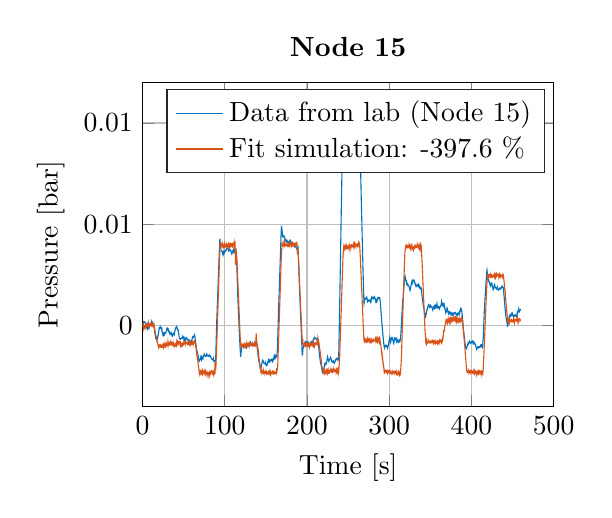
\begin{tikzpicture}

\begin{axis}[%
scaled y ticks = false,
 y tick label style={/pgf/number format/fixed,
/pgf/number format/1000 sep = \thinspace}, % Optional if you want to replace comma as the 1000 separator 
width=2.0556in,
height=1.62135in,
at={(1.011in,0.642in)},
scale only axis,
xmin=0,
xmax=500,
xlabel={Time [s]},
xmajorgrids,
ymin=-0.004,
ymax=0.012,
ylabel={Pressure [bar]},
ymajorgrids,
axis background/.style={fill=white},
title style={font=\bfseries},
title={Node 15},
legend style={legend cell align=left,align=left,draw=white!15!black}
]
\addplot [color=mycolor1,solid]
  table[row sep=crcr]{%
0.05	-7.60719452591041e-05\\
1.15	0.000148385532746709\\
1.45	0.000202324926686037\\
2.45	0.000192755034213107\\
3.25	0.000122285826002044\\
3.3	0.000125765786901322\\
4.3	1.35718475061108e-06\\
5.1	-0.000107391593352768\\
5.35	-0.000103041642228574\\
5.8	-0.000170900879765165\\
6.7	-9.08617790808808e-05\\
7.3	-0.000146541153470126\\
7.5	-0.000136971260997029\\
8.55	-4.56222873901069e-05\\
9.6	4.65966764417458e-05\\
10.6	0.000140555620723126\\
10.8	0.000196234995112149\\
11.4	0.000107495992179615\\
11.95	0.000150125513196042\\
12.4	8.22662756596038e-05\\
13.1	9.79260997066578e-05\\
13.85	-9.08269794719363e-06\\
14.9	-0.000329239100683956\\
15.85	-0.000596326099706543\\
15.95	-0.000590236168132668\\
17.05	-0.000646785532746122\\
17.1	-0.000650265493645483\\
17.45	-0.000569356402736365\\
18.1	-0.000644175562071428\\
19.05	-0.00043972785923671\\
19.2	-0.000441467839686474\\
20.15	-0.000156981036167389\\
20.3	-0.000172640860214221\\
21.25	-6.82420332351608e-05\\
21.5	-4.91022482888848e-05\\
21.95	-0.000123921407624572\\
23.1	-0.000101301661779657\\
23.35	-0.000179600782014441\\
23.45	-0.000165680938417193\\
24.45	-0.000405798240470212\\
25.05	-0.000507587096775119\\
25.55	-0.00049018729227869\\
25.95	-0.000383178494624853\\
26.55	-0.000431027956990182\\
27	-0.000350118866080718\\
28.15	-0.000377958553275104\\
28.7	-0.000297919452590556\\
29.45	-0.000159591006842263\\
30.15	-0.000198740566959649\\
30.55	-0.0001247913978496\\
31.2	-0.000156981036168458\\
31.85	-0.000285739589442197\\
32.15	-0.000270949755620378\\
32.95	-0.000383178494622993\\
33	-0.000388398435971937\\
33.25	-0.000343158944280761\\
34.6	-0.000424068035189962\\
34.95	-0.000375348582599175\\
35.05	-0.000399708308894131\\
36.05	-0.000522376930595064\\
36.4	-0.000529336852393952\\
36.85	-0.000423198044964865\\
37.15	-0.000429287976538462\\
37.5	-0.000378828543498522\\
38.55	-0.000451037732159709\\
39.3	-0.000265729814271434\\
40.35	-0.000109131573802768\\
41.4	-3.77923753659831e-05\\
42.3	-0.000169160899315665\\
42.6	-0.000152631085044166\\
43.5	-0.000257899902248504\\
43.55	-0.000256159921798838\\
44.6	-0.000580666275660058\\
45.65	-0.00067462521994141\\
45.85	-0.00067723519061566\\
46.7	-0.000631125708700359\\
46.9	-0.000633735679374609\\
47.3	-0.000602416031280945\\
48.25	-0.000619815835777013\\
48.8	-0.000546736656891617\\
49	-0.000520636950146813\\
49.9	-0.000624165786900222\\
50.3	-0.000681585141738883\\
50.65	-0.000614595894427264\\
50.95	-0.000655485434994246\\
51.7	-0.000748574389050308\\
52	-0.000736394525902573\\
52.9	-0.000585016226781504\\
53.55	-0.000593716129029531\\
53.95	-0.000633735679371944\\
54.1	-0.000630255718472764\\
54.45	-0.000701594916909368\\
55.2	-0.00069463499511066\\
56.25	-0.00079207390029154\\
56.7	-0.000726824633428894\\
57.3	-0.000803383773214705\\
58.05	-0.000919092473117292\\
58.4	-0.000882552883674059\\
59.4	-0.000753794330398988\\
59.65	-0.000757274291298515\\
60.45	-0.000622425806451263\\
60.5	-0.000622425806451443\\
61.05	-0.000540646725318006\\
61.75	-0.000573706353861531\\
61.9	-0.000543256695992256\\
62.6	-0.000545866666667394\\
63.1	-0.000454517693061013\\
63.65	-0.000510197067450341\\
64.7	-0.000860803128055143\\
65.8	-0.00121575913978386\\
66.85	-0.00132885786901273\\
67.9	-0.00154809540566855\\
68.7	-0.00176559296187506\\
69.15	-0.00174732316715354\\
70	-0.00167250400781899\\
70.95	-0.00153069560117196\\
71.1	-0.00157419511241301\\
71.7	-0.00167250400781864\\
72.35	-0.00155331534701669\\
73.1	-0.00163770439882527\\
73.3	-0.00164553431084855\\
74.25	-0.0014741462365593\\
75	-0.00140106705767462\\
75.3	-0.00143499667644306\\
76.1	-0.00149937595308219\\
77.2	-0.00151416578690508\\
77.45	-0.00145326647116725\\
78.05	-0.00139671710655229\\
78.45	-0.00145848641251504\\
78.65	-0.00145239648094125\\
79.55	-0.00149763597263217\\
79.9	-0.00146979628543768\\
80.4	-0.00150024594330801\\
80.85	-0.00150981583578044\\
81.7	-0.00145152649071811\\
82.75	-0.00153417556207877\\
83.8	-0.00161160469208951\\
84.85	-0.0016855538611977\\
85.7	-0.00169599374389257\\
85.9	-0.00166467409579801\\
86.15	-0.00161421466275719\\
87	-0.00176559296187719\\
87.4	-0.0017334033235577\\
88.7	-0.00176559296187612\\
89.1	-0.00146544633431127\\
90.15	0.000122285826000101\\
91.2	0.00126371300097297\\
92.3	0.00247560938415931\\
93.35	0.00367706588464792\\
94.05	0.00429127898337754\\
94.4	0.0041303307917844\\
95.45	0.00370229560116904\\
96.5	0.00366749599217797\\
96.9	0.00367445591397597\\
97.6	0.00353438748777968\\
97.75	0.00349784789833769\\
98.5	0.00362834643206121\\
98.95	0.00356135718474888\\
99.7	0.00365183616813142\\
99.9	0.00362312649071164\\
100.7	0.00371273548386852\\
101.3	0.00369272570869697\\
101.8	0.0037318752688148\\
102.75	0.00382235425219662\\
103.1	0.00387542365591187\\
103.7	0.0038119143695014\\
103.95	0.00382235425219982\\
104.7	0.00368228582600211\\
105.4	0.00369446568915002\\
105.8	0.00374840508308949\\
106.3	0.00375623499511313\\
107.1	0.00369098572825032\\
107.5	0.00369620566959811\\
108.15	0.00357788699902073\\
108.45	0.00354569736070232\\
108.8	0.00360572668621593\\
109.25	0.00359528680351716\\
110.3	0.00375536500488644\\
110.35	0.00375971495601071\\
111.3	0.00361094662756478\\
111.35	0.00361703655913857\\
112.3	0.00377102482893371\\
112.4	0.00373709521016508\\
113.25	0.00361877653958737\\
113.5	0.00365966608015399\\
114.55	0.00316203167155188\\
115.6	0.00166390850439704\\
116.65	0.000646019941347553\\
117.7	-0.000314449266861347\\
118.75	-0.00120009931573641\\
119.35	-0.00153069560117089\\
119.85	-0.00129927820136679\\
120.9	-0.000995651612902576\\
121.15	-0.000958242033235301\\
121.5	-0.00102697126099677\\
121.95	-0.00101914134897385\\
122.8	-0.00095650205278687\\
123.25	-0.0010078314760537\\
123.9	-0.0009547620723388\\
124.85	-0.000942582209190163\\
125.15	-0.00098956168133163\\
126.15	-0.00112093020528008\\
126.2	-0.00112093020528008\\
127.25	-0.00095737204301144\\
127.8	-0.000965201955036146\\
128.3	-0.000925182404695163\\
128.75	-0.000960852003913645\\
129.35	-0.000894732746825888\\
130.05	-0.000915612512221317\\
130.45	-0.000854713196482421\\
131.15	-0.000818173607039729\\
131.5	-0.000903432649073041\\
132.35	-0.000962591984361008\\
132.75	-0.000949542130988523\\
133.5	-0.000918222482893249\\
133.8	-0.000894732746823765\\
134.6	-0.000974771847508937\\
134.85	-0.000986081720430146\\
135.6	-0.000926052394917956\\
135.75	-0.000936492277615664\\
136.7	-0.000807733724339885\\
136.9	-0.000854713196480644\\
137.8	-0.000812083675462386\\
138.2	-0.000807733724339177\\
138.9	-0.000899952688169781\\
139.95	-0.00128709833821851\\
141.05	-0.00165336422287325\\
142.1	-0.0018621618768335\\
143.15	-0.00206921955034424\\
143.75	-0.00217622834799862\\
144.2	-0.00204398983382525\\
145.25	-0.00183867214076898\\
146.05	-0.00169860371456948\\
146.35	-0.00171078357771741\\
147.35	-0.00182301231671993\\
147.45	-0.00181344242424679\\
148.45	-0.00187434173998532\\
148.7	-0.00187260175953476\\
149.4	-0.00190131143695275\\
149.6	-0.00183780215053979\\
150.45	-0.00196047077224108\\
151.1	-0.00197787057673857\\
151.65	-0.00190044144672746\\
151.7	-0.00190653137830125\\
152.7	-0.00174645317693234\\
153.1	-0.00168903382209351\\
153.7	-0.00176907292277867\\
154	-0.00172296344086248\\
154.8	-0.00178299276637539\\
155.3	-0.00168120391007058\\
156.65	-0.00171513352883779\\
156.9	-0.00166554408602224\\
157.3	-0.00164988426197674\\
157.9	-0.00178560273705158\\
158.1	-0.00177429286412824\\
158.7	-0.00167076402737251\\
159.15	-0.0016803339198485\\
159.9	-0.00152808563050144\\
160.35	-0.00159855483871205\\
161.1	-0.00146892629521098\\
161.15	-0.00147762619745884\\
161.95	-0.00159420488758848\\
162.25	-0.00157332512219199\\
162.75	-0.00147588621701039\\
163.55	-0.00149502600195739\\
164.35	-0.000789463929618178\\
165.4	0.000773038514173485\\
166.45	0.00198580488758189\\
167.5	0.00327687038122881\\
168.6	0.0046610248289327\\
169	0.00492289188660784\\
169.65	0.00469495444770025\\
170.7	0.00437044809384098\\
170.75	0.00436957810361641\\
171.65	0.00444091730205408\\
171.8	0.00443656735092908\\
172.8	0.00435652825024427\\
173.6	0.00419384007820163\\
174.25	0.00423994956011675\\
174.95	0.00417905024438106\\
175.25	0.00414251065493765\\
175.8	0.00419471006842549\\
176	0.00417557028347922\\
177.05	0.00407465141739827\\
177.15	0.00405725161290256\\
178.05	0.00415469051808096\\
178.5	0.00418253020527296\\
179.2	0.00408857126098645\\
179.85	0.00418601016616769\\
180.25	0.00413381075267771\\
181.1	0.00399461231670351\\
181.3	0.00403289188659678\\
181.9	0.00410162111436002\\
182.35	0.00408074134896602\\
183.4	0.00398939237536033\\
183.45	0.00398417243401149\\
184.2	0.00404507174975642\\
184.5	0.00400505219941401\\
185	0.0039023933528825\\
185.8	0.00396155268816763\\
186.45	0.00388673352883523\\
186.6	0.00389456344085709\\
187.4	0.00379886451612499\\
188	0.00375275503420987\\
188.7	0.00385280391006625\\
189.05	0.00388151358748423\\
189.8	0.00309678240468976\\
190.85	0.00189271593353063\\
191.9	0.000847857673509436\\
192.95	-0.000138711241448347\\
194	-0.00126969853372565\\
194.4	-0.00147153626588753\\
195.1	-0.00114963988269984\\
196.15	-0.000989561681330214\\
196.25	-0.00100261153470235\\
197.2	-0.000876462952099574\\
197.5	-0.000808603714560902\\
198.25	-0.000822523558156901\\
198.75	-0.000775544086014365\\
199.3	-0.000796423851408365\\
200	-0.000872113000966762\\
200.6	-0.000851233235571347\\
201.3	-0.000794683870957796\\
201.45	-0.000804253763429519\\
202.4	-0.000989561681321693\\
202.95	-0.000944322189633973\\
203.4	-0.000996521603123246\\
203.75	-0.00101218142717194\\
204.6	-0.000895602737046558\\
205.15	-0.000786853958944456\\
205.75	-0.000825133528837729\\
206.55	-0.000785983968721315\\
206.75	-0.000804253763443008\\
207.75	-0.000686805083088798\\
207.95	-0.000698984946236367\\
208.75	-0.000596326099705557\\
208.85	-0.000618075855324848\\
209.3	-0.00064678553274497\\
210.3	-0.000605895992176572\\
210.95	-0.000648525513190557\\
211.3	-0.000637215640267572\\
212.05	-0.0006946349951064\\
212.5	-0.000761624242417658\\
213.2	-0.000697244965779401\\
214.15	-0.000993911632444555\\
215.2	-0.00144456656890732\\
216.25	-0.00177864281524684\\
217.35	-0.00198048054740801\\
218.4	-0.00221537790811716\\
218.8	-0.00232238670577012\\
219.45	-0.00228845708699971\\
220.4	-0.00213359882697822\\
220.5	-0.00214142873900151\\
221.55	-0.00188304164222536\\
221.7	-0.00188826158357351\\
222.4	-0.00184476207233281\\
222.95	-0.00183432218963439\\
223.2	-0.00190044144672036\\
223.7	-0.00184650205278196\\
224.75	-0.00159942482893377\\
225.05	-0.00153678553274467\\
225.8	-0.00166902404692017\\
226.55	-0.00176211300097499\\
226.85	-0.00171861348973287\\
227.95	-0.00162552453567094\\
228.55	-0.00155505532745998\\
229.35	-0.00161943460409823\\
230	-0.00175341309872572\\
230.25	-0.0017490631475993\\
231.05	-0.00179343264906456\\
231.1	-0.00178734271749115\\
232.05	-0.0017351433040033\\
232.15	-0.00173949325512758\\
233.15	-0.00185433196481163\\
233.5	-0.0018543319648095\\
234.3	-0.00173427331378441\\
234.35	-0.00174558318670741\\
235.35	-0.00168033391984601\\
236.4	-0.00160203479961105\\
236.55	-0.00159855483871134\\
237.4	-0.00168207390029657\\
237.75	-0.00171078357771598\\
238.55	-0.00160377478005735\\
239.6	0.000622530205281968\\
240.65	0.00313767194526456\\
241.7	0.00568239335288759\\
242.75	0.00812097595308295\\
243.85	0.0100967237536687\\
243.95	0.0101297833822124\\
244.9	0.0098722662756608\\
245.95	0.00980179706744772\\
246	0.00980875698924642\\
246.8	0.00969217829911749\\
247.05	0.00970435816226434\\
248.05	0.00983311671553658\\
248.6	0.00993751554251439\\
249.15	0.00980701700878804\\
250.2	0.00968782834798823\\
250.6	0.00974698768327478\\
251.25	0.00961735913977656\\
251.85	0.00966085865101939\\
252.3	0.00958864946235856\\
252.55	0.00959038944280913\\
253.25	0.00950078044965615\\
253.35	0.00952949012707485\\
254.3	0.0097234979472092\\
255.3	0.00972610791788434\\
255.5	0.00968260840664151\\
255.75	0.00965824868034637\\
256.5	0.00979483714564544\\
256.55	0.00979048719452116\\
257.6	0.00967738846529194\\
258.55	0.00954166999021673\\
258.7	0.00955384985336571\\
259.35	0.00946946080156302\\
259.7	0.00949208054740758\\
260.8	0.00957385962854368\\
260.95	0.00957994956011568\\
261.6	0.00946250087976218\\
261.95	0.00950687038122744\\
262.8	0.00956167976539397\\
262.9	0.00955210987292084\\
263.55	0.00963736891495309\\
263.95	0.00955384985336927\\
265	0.00807225650048203\\
266.1	0.00610868856304457\\
267.15	0.00434782834799285\\
268.2	0.00268179706744653\\
269.25	0.0011436543499493\\
269.4	0.00108014506353704\\
270.3	0.00130199257086908\\
270.8	0.00135332199413235\\
272	0.00131678240469178\\
272.45	0.0013916015640249\\
272.75	0.00141074134897046\\
273.5	0.00122456344085727\\
273.7	0.00118280391006642\\
274.55	0.00124283323557756\\
274.65	0.00125675307917568\\
275.35	0.00121847350928171\\
276.05	0.00124892316715026\\
276.65	0.0012193434995077\\
276.9	0.00125240312804997\\
277.65	0.00115061427174445\\
277.75	0.00117062404691459\\
278.8	0.00142205122188421\\
279.85	0.00137072179862451\\
280.3	0.00139073157379677\\
280.65	0.00131765239491351\\
281.1	0.00132635229715923\\
282	0.00140639139784049\\
282.15	0.00142118123166249\\
283.05	0.0013211323558118\\
283.65	0.00119585376343785\\
284.1	0.00125414310849913\\
284.65	0.00116801407624018\\
285.15	0.00120194369500702\\
286.2	0.00139421153469364\\
286.4	0.00139508152491821\\
287	0.00133679217985623\\
287.65	0.00135506197458149\\
287.85	0.00139247155424804\\
288.6	0.00136637184750164\\
289.4	0.00103838553274407\\
290.45	0.000438962267838933\\
291.5	-7.17219941356734e-05\\
292.6	-0.000560656500492418\\
293.65	-0.00098782170087823\\
294.25	-0.0010983104594316\\
294.7	-0.00103480117302147\\
295.35	-0.000956502052788646\\
296.05	-0.000956502052788646\\
296.25	-0.00100696148582947\\
296.8	-0.00098173176931049\\
297.8	-0.00108178064516544\\
298.05	-0.00111049032258485\\
298.95	-0.000970421896388907\\
300	-0.000724214662761749\\
300.75	-0.000582406256116663\\
301.05	-0.00067375522972235\\
301.7	-0.000817303616818699\\
302.1	-0.000744224437930471\\
303	-0.000588496187684417\\
303.85	-0.000581536265882865\\
304.25	-0.000680715151511815\\
304.35	-0.000678105180837385\\
305.3	-0.000870373020519746\\
305.45	-0.000885162854340316\\
306.35	-0.000694634995104262\\
306.75	-0.00059545610947459\\
307.9	-0.000613725904199849\\
308.45	-0.000723344672530074\\
308.55	-0.000701594916910797\\
308.85	-0.000779894037143625\\
309.7	-0.000680715151513245\\
310.35	-0.000775544086019334\\
310.6	-0.000764234213094211\\
311.2	-0.000821653567932332\\
311.65	-0.00079729384163435\\
312.1	-0.000710294819151538\\
312.9	-0.000781634017588503\\
313.75	-0.000665055327464539\\
314.85	6.92164222883956e-05\\
315.9	0.00090353704789628\\
316.95	0.00139595151514776\\
318	0.00198754486803317\\
319.05	0.00243906979471908\\
319.2	0.00246168954056508\\
320.15	0.00228682150537558\\
321.2	0.00208585376343827\\
321.45	0.00212587331378067\\
322	0.00205540410556758\\
322.25	0.00205540410556758\\
322.5	0.00198493489735448\\
323.3	0.00200233470185303\\
324.35	0.00189445591397551\\
325.35	0.00173524770282973\\
325.45	0.00174481759530287\\
326.5	0.00198145493645974\\
327.5	0.00216937282502493\\
328.1	0.00210760351906039\\
328.6	0.00221461231671477\\
328.9	0.00217981270772263\\
329.15	0.00222244222873876\\
330	0.00225550185728246\\
330.75	0.00218503264907007\\
331.8	0.00200842463342646\\
332.45	0.00195448523948592\\
332.75	0.0020110346041016\\
333.3	0.00196492512218505\\
333.9	0.00199711476050063\\
334.6	0.00202495444769404\\
334.95	0.00195187526880509\\
335	0.00194665532745625\\
335.8	0.00202756441836137\\
336.05	0.00199363479959735\\
336.65	0.00189271593351997\\
337.1	0.00193099550341252\\
338.05	0.00182920664710345\\
338.55	0.00180223695013459\\
338.85	0.00184747644183013\\
339.2	0.00180919687193615\\
340.25	0.00133766217008152\\
341.35	0.00104360547409364\\
342.4	0.000792178299121885\\
343.45	0.000559020918862604\\
344.2	0.000449402150533795\\
344.5	0.000482461779078916\\
345.5	0.000706919257091057\\
345.55	0.000699959335291642\\
346.6	0.000874827370475451\\
346.7	0.000866127468226882\\
347.65	0.00102620566959509\\
348	0.0010444754643175\\
348.75	0.000981836168136921\\
349.3	0.000907886999023402\\
350.2	0.000994016031275247\\
350.65	0.000933116715539556\\
351.35	0.00090962697946971\\
351.7	0.000942686608011986\\
352	0.000933116715535295\\
353	0.000773038514168503\\
354.05	0.000915716911041004\\
354.5	0.000957476441830418\\
355.1	0.000881787292270605\\
355.15	0.000873957380245899\\
355.95	0.00101141583576386\\
356.15	0.000992276050820418\\
356.9	0.000886137243395591\\
357.25	0.000918326881715434\\
358.05	0.0010879749755518\\
358.3	0.00102011573801526\\
358.8	0.0008887472140615\\
359.95	0.000938336656879882\\
360.35	0.000876567350921745\\
360.9	0.000831327859238298\\
361.45	0.000932246725315694\\
362.05	0.000926156793748661\\
362.5	0.000978356207237213\\
362.75	0.000967916324542351\\
363.6	0.00113843440860258\\
363.75	0.00118628387096897\\
364.55	0.00104099550342206\\
364.8	0.00107753509286689\\
365.4	0.0010262056696022\\
365.75	0.00106187526881463\\
366.45	0.000952256500484416\\
366.9	0.00103055562071297\\
367.7	0.00084872766372833\\
367.8	0.000859167546424622\\
368.9	0.000635580058651969\\
369.95	0.000773038514181298\\
370.4	0.000856557575760142\\
371	0.000742588856310608\\
371.15	0.000766078592379038\\
372.05	0.000628620136858229\\
372.45	0.000579030694038418\\
373.1	0.000679949560120074\\
373.35	0.000687779472143366\\
374	0.000611220332358262\\
374.45	0.000635580058653384\\
375.15	0.000528571261001864\\
375.35	0.000529441251229987\\
375.85	0.000606000391022196\\
376.65	0.000529441251238508\\
377.35	0.000585120625629612\\
377.45	0.000599910459450903\\
378.15	0.000517261388095921\\
378.4	0.000545101075290766\\
378.9	0.000624270185748871\\
379.5	0.00061209032259775\\
380.4	0.000658199804510748\\
380.65	0.000647759921810195\\
381.55	0.000530311241453849\\
381.75	0.000523351319655849\\
382.65	0.000583380645166262\\
382.95	0.000541621114374002\\
383.15	0.000593820527866815\\
383.7	0.000565980840673386\\
384.8	0.000643409970682352\\
385.05	0.000664289736077781\\
385.3	0.000584250635390124\\
385.85	0.000652109872926659\\
386.7	0.00082262795699542\\
387.2	0.000769558553283006\\
387.75	0.000816538025419866\\
387.95	0.000795658260023022\\
389	0.000467671945250533\\
390.1	-0.000130881329434299\\
391.15	-0.000491927272734852\\
392.2	-0.000859933137844771\\
393.2	-0.00111223030304324\\
393.75	-0.00114006999023239\\
394.3	-0.00109048054741401\\
395.4	-0.000949542130999181\\
395.95	-0.000849493255148492\\
396.5	-0.000895602737058632\\
397.4	-0.00082948347997551\\
397.85	-0.000770324144684698\\
398.55	-0.000837313391997371\\
398.7	-0.000834703421321525\\
398.95	-0.000866023069414648\\
399.65	-0.00084862326491042\\
400.3	-0.000774674095801162\\
401.2	-0.000748574389051196\\
401.75	-0.000833833431086284\\
401.85	-0.000817303616814438\\
402.7	-0.000880812903228834\\
402.8	-0.000863413098731697\\
403.25	-0.000805123753667591\\
403.85	-0.000858193157384265\\
404.9	-0.000961721994138923\\
405	-0.00095824203323637\\
406	-0.00111745024438215\\
406.1	-0.00113833000978182\\
406.6	-0.00105742091887315\\
407.3	-0.00105046099707656\\
407.85	-0.00110875034214068\\
408.15	-0.00107743069404329\\
409	-0.00101827135876099\\
409.2	-0.00101827135875958\\
409.95	-0.00107569071360267\\
410.5	-0.00105655092866208\\
411.25	-0.000963461974600857\\
411.35	-0.000956502052802857\\
411.75	-0.00100783147606755\\
412.4	-0.00095998201369546\\
413.4	-0.00108265063540636\\
413.45	-0.00108526060607936\\
414.45	-0.000552826588483338\\
415.5	0.000590340566951467\\
416.55	0.00135593196480109\\
417.65	0.00203713431083663\\
418.7	0.00268527702833132\\
418.9	0.00274008641249573\\
419.75	0.00249300918864755\\
420.8	0.00218764261973242\\
421.85	0.0021337032257933\\
421.95	0.00213805317691829\\
422.95	0.00195622521994501\\
423.15	0.00194317536657429\\
424	0.00208411378299907\\
424.6	0.00210673352884222\\
425.05	0.00204235425219829\\
426.1	0.00186226627565994\\
426.4	0.00178309716519898\\
427.1	0.0018683562072298\\
427.2	0.00185878631475739\\
428.15	0.00202930439882046\\
428.3	0.00201364457477389\\
429.1	0.0018840160312707\\
429.3	0.00188488602149739\\
430.3	0.0018144168132907\\
430.65	0.00180223695014668\\
431.4	0.00189967585532863\\
431.45	0.00190924574780248\\
432.45	0.00179527702834868\\
432.75	0.00175003753665387\\
433.55	0.00178309716519472\\
434.5	0.00184834643205115\\
435	0.00181789677418046\\
435.35	0.00185008641250028\\
435.8	0.00183007663733015\\
436.7	0.00190315581620559\\
437.1	0.00189010596283345\\
437.4	0.00195796520037142\\
437.75	0.00193882541542799\\
438.85	0.00186400625609628\\
439.9	0.00136550185727209\\
440.95	0.000843507722378053\\
442	0.000432002346042348\\
442.05	0.000432002346043778\\
443.05	0.000184925122191329\\
444	-2.03925708773811e-05\\
444.15	-1.51726295285204e-05\\
445.2	0.000187535092860069\\
446.25	0.000423302443788104\\
446.75	0.000519871358747606\\
447.7	0.000467671945263315\\
448.35	0.00055206099707597\\
448.55	0.000585120625618246\\
449.1	0.00053292121212685\\
449.8	0.000606870381238953\\
450.5	0.000488551710668694\\
450.85	0.000499861583587419\\
451.5	0.000419822482898347\\
451.55	0.000419822482898347\\
451.95	0.000522481329431987\\
452.95	0.000545101075266605\\
453.65	0.000461582013686346\\
453.75	0.000459842033237193\\
454.4	0.000492901661783729\\
454.85	0.000459842033240038\\
455.6	0.000630360117300277\\
455.9	0.000580770674484726\\
456.7	0.000693869403710398\\
456.9	0.000688649462361537\\
457.65	0.000832197849453639\\
457.9	0.000765208602143796\\
458.35	0.000700829325508398\\
460	0.00081392805473833\\
};
\addlegendentry{Data from lab (Node 15)};

\addplot [color=mycolor2,solid]
  table[row sep=crcr]{%
0.05	0.000199585146030196\\
1.05	-0.000121690200085692\\
1.15	-9.81430039181283e-05\\
1.35	1.55387520991294e-05\\
2.4	-0.000103597430204942\\
3.2	1.93690528975687e-05\\
3.9	5.28387177407175e-05\\
4	-5.26524758767747e-05\\
4.45	2.67867013814627e-05\\
4.7	-4.14280434566252e-05\\
5.6	-2.54448356855389e-05\\
6	7.96306551660029e-05\\
6.8	-3.39596812430582e-05\\
7.25	9.80222945143379e-05\\
7.5	-1.4024948184652e-05\\
8.25	6.64199632313186e-05\\
8.7	-3.50721428891168e-05\\
9.1	5.26625362417878e-05\\
9.7	0.000100199995900232\\
10.65	2.12245902451063e-05\\
11.25	-2.22648419852618e-05\\
11.6	7.14354165141818e-05\\
11.85	4.07903670155015e-06\\
12.5	9.72815277972126e-05\\
13.35	7.86270342512413e-05\\
13.6	1.18328044993925e-05\\
14	6.37372467556515e-05\\
14.7	-0.000180050995651215\\
14.9	-0.000169011919863334\\
15.95	-0.000469367238522032\\
17.05	-0.000689014358238691\\
17.2	-0.000663752991804985\\
18.1	-0.000840863450753475\\
18.25	-0.000834171861582276\\
19.15	-0.00101974890375823\\
19.55	-0.00107623189562761\\
20.15	-0.000909095832644425\\
20.2	-0.000945875186044244\\
21.25	-0.00102858713048573\\
21.3	-0.00103667891887993\\
22.1	-0.000937184597785223\\
22.4	-0.000951329487209038\\
22.8	-0.00106106288402753\\
24.05	-0.00107379317341414\\
24.3	-0.000966857644703295\\
24.65	-0.00092984236896103\\
25.3	-0.00106810765440987\\
26.1	-0.000910644587940296\\
26.45	-0.00103429758581183\\
27.05	-0.00105876104641213\\
27.65	-0.000897110334090106\\
27.7	-0.000894021458446823\\
28.4	-0.000998612090147728\\
28.8	-0.00087826272000883\\
29.3	-0.000980305607142569\\
30.4	-0.000985189948363381\\
30.8	-0.000832012229775927\\
31.05	-0.000935435238651894\\
31.4	-0.000816619730920526\\
32.4	-0.000815338049786118\\
32.7	-0.000958741470041809\\
33.8	-0.000934769739713514\\
34	-0.000834413147992278\\
34.15	-0.000803266982258443\\
34.8	-0.000902862806654443\\
35.15	-0.000842072579410544\\
35.85	-0.00094307230170474\\
36.35	-0.000952730728925529\\
37.05	-0.000840064641845808\\
37.15	-0.000875431117131189\\
37.6	-0.000977650092620462\\
38.25	-0.000896047883102532\\
39.15	-0.00103386022034883\\
40.1	-0.00100307964469609\\
40.25	-0.000915653819829668\\
40.7	-0.000949251922903536\\
41.4	-0.000849592876386819\\
41.45	-0.000835001980875481\\
41.65	-0.000948352793908473\\
42.7	-0.000789464902402235\\
43.3	-0.000916944681454389\\
43.7	-0.000864154566760255\\
44.2	-0.000788817057210758\\
44.85	-0.000783621272406916\\
45.45	-0.000912829919457213\\
45.8	-0.00083413094837229\\
46.45	-0.00097423017066281\\
46.7	-0.00090730856350701\\
47.25	-0.000984575961301689\\
47.95	-0.000903020179773301\\
48.65	-0.00098932219962894\\
48.95	-0.000958120945359633\\
49.55	-0.000834565921545316\\
49.9	-0.000914252688792538\\
50.95	-0.000833048565829975\\
51.35	-0.000880611088042316\\
51.95	-0.000805279358745825\\
52.05	-0.000879076762085664\\
52.5	-0.00079954732711843\\
53.4	-0.000813389996832328\\
54.05	-0.00090762331746902\\
54.55	-0.000928090451949138\\
54.85	-0.000829799617734255\\
55.55	-0.000841264108952801\\
56	-0.000916177384399078\\
56.35	-0.000909305599912049\\
56.7	-0.000812499980997967\\
57.5	-0.000941625884929965\\
58.1	-0.00084040785877735\\
58.5	-0.000894758003497551\\
58.65	-0.000768759853041312\\
59.55	-0.000825181799373973\\
59.85	-0.000913579606522747\\
60.75	-0.000904109251272169\\
61.1	-0.00080890189696676\\
61.65	-0.000930296128626109\\
62.35	-0.000803743178012699\\
62.75	-0.000821475579372275\\
63.15	-0.000759211611029088\\
63.7	-0.00080897405308314\\
64.55	-0.000984441127180251\\
64.7	-0.000967475598150179\\
65.6	-0.00130583089366269\\
65.8	-0.00125182834387194\\
66.8	-0.00166195936724871\\
66.85	-0.00162918158787311\\
67.9	-0.00194624667135268\\
68.95	-0.00229871154806317\\
69.05	-0.00225679804506424\\
69.45	-0.00235696456876299\\
70.1	-0.00239403161470563\\
70.6	-0.00225706800196111\\
71.4	-0.00234120507780832\\
71.75	-0.00225878474095349\\
72.8	-0.00238245359452981\\
73.05	-0.00221859203693299\\
73.2	-0.00223501457517112\\
74.25	-0.00233766374988867\\
74.65	-0.00236319763973409\\
74.9	-0.00224611809466243\\
75.5	-0.00219818097869249\\
76.3	-0.00237879012533553\\
76.8	-0.00228097315428053\\
77.1	-0.00237568061004249\\
78.3	-0.00228573875342423\\
78.5	-0.00237370975061177\\
78.65	-0.00244327033768335\\
79.35	-0.00231416464101161\\
80.1	-0.00230473409346558\\
80.5	-0.00242466658617467\\
80.7	-0.00235910299425691\\
81.6	-0.00229388988285828\\
81.8	-0.00238196589896464\\
82.1	-0.00227993828341259\\
82.75	-0.00236256830298065\\
83.65	-0.00224432616863615\\
83.95	-0.00227058803351451\\
84.65	-0.00234380234772968\\
84.95	-0.00227146903350463\\
85.9	-0.00237241096788533\\
86.35	-0.00230446261005384\\
86.6	-0.00239916572257151\\
87.05	-0.00230424501694458\\
87.35	-0.00238175765678067\\
88.1	-0.00235016776261716\\
88.15	-0.00181646759400929\\
89.1	-0.00216739319569978\\
90.15	-0.00102933433108876\\
91.2	0.000276217384706972\\
92.3	0.00163142740642237\\
93.35	0.00293768878940947\\
94.25	0.00398881607733097\\
94.7	0.00403900761103333\\
94.9	0.00395927845975604\\
95.8	0.00402012896689315\\
96.4	0.00390852918768108\\
97	0.00389185042989061\\
97.2	0.0040400205877331\\
97.6	0.00398159670742967\\
97.8	0.00389338394712924\\
98.95	0.00399626241765417\\
99.1	0.00386962680344864\\
99.95	0.00403547422181508\\
100.15	0.00386591472955293\\
101.55	0.00390766065641894\\
101.8	0.00400065638704058\\
102.05	0.00402069854050537\\
102.4	0.00389021651807986\\
103.15	0.00388993874321452\\
103.7	0.00400309227111521\\
104.35	0.00405671741605033\\
104.95	0.00388446277579558\\
105	0.00390501773470328\\
105.45	0.00399724425277814\\
106.3	0.00387490612763159\\
106.7	0.0040077634858256\\
107.2	0.00395562275523105\\
107.75	0.00404508098970128\\
108.25	0.00404695228979716\\
108.65	0.00390098780561156\\
109.4	0.00388065890521136\\
109.75	0.00405292674956648\\
110.7	0.00408386778176343\\
111.1	0.0039802810666429\\
111.35	0.00407052027256564\\
111.65	0.00393844940184986\\
112.45	0.00405122361127503\\
113.15	0.0029909461916601\\
113.65	0.0038091296185339\\
114.55	0.00342107619316981\\
115.6	0.00247727542947582\\
116.65	0.00149400378219006\\
117.7	0.000448709017495688\\
118.75	-0.000557692342413487\\
119.6	-0.000975931230259873\\
119.85	-0.000899186459228912\\
120.5	-0.00103528969854545\\
121.15	-0.00101314979380615\\
121.3	-0.000932027411283062\\
122.5	-0.000922832032158874\\
122.7	-0.0010066166156897\\
123.2	-0.000934274108576257\\
123.85	-0.00106203660603821\\
124.5	-0.00100424315650598\\
124.65	-0.000914910596275134\\
125.6	-0.00101555060400923\\
126.1	-0.000902648999366868\\
126.3	-0.00100782791692147\\
126.6	-0.000902384097109373\\
127.5	-0.0009948471062417\\
128.3	-0.000868837162385303\\
129	-0.000989445416545732\\
130.05	-0.000874202483989316\\
130.25	-0.000964270278813862\\
130.6	-0.000888900054052404\\
131.1	-0.000972869146067682\\
131.85	-0.000965759439427366\\
132.35	-0.000899711731331461\\
133.15	-0.00098456594353374\\
133.45	-0.000927838321064535\\
133.95	-0.000864347636407411\\
134.35	-0.00098681728866186\\
135.05	-0.000975024996543693\\
135.7	-0.000887596035067388\\
135.8	-0.000879166860434087\\
136.35	-0.00096767024911408\\
137.1	-0.000890605451529593\\
137.35	-0.000969609125278919\\
137.85	-0.000916781749201686\\
138.15	-0.000375712191142923\\
138.9	-0.00079737512038305\\
139.95	-0.00109327931920577\\
140.05	-0.00107855690674138\\
140.95	-0.00139462227602818\\
141.05	-0.00135718224743713\\
142.1	-0.00174542067237619\\
143.05	-0.00204515871767303\\
143.15	-0.00201663212559798\\
144.2	-0.00228793973206935\\
144.4	-0.00221675482920297\\
144.75	-0.00230025535749059\\
145.8	-0.00223659529314511\\
146.15	-0.00235528345190626\\
147.05	-0.00234324015965226\\
147.15	-0.0022364887978635\\
147.75	-0.00234757075165266\\
148.05	-0.00224440080231207\\
148.75	-0.00224643271528533\\
149.35	-0.00234281596338109\\
150.1	-0.00231796722706814\\
150.4	-0.00224591788741221\\
150.7	-0.00227905550724743\\
150.85	-0.00239700486366403\\
152.15	-0.00235687006138896\\
152.3	-0.00229516234366311\\
152.75	-0.00227405520787528\\
153.05	-0.00238544923628066\\
154	-0.00238288581037088\\
154.25	-0.00226555810197658\\
155.1	-0.00239326860183377\\
155.8	-0.00227830209999901\\
156.15	-0.00236813713936863\\
156.45	-0.00229205274917279\\
157.3	-0.0023356596264246\\
158	-0.00226501074024396\\
158.7	-0.00235900243986643\\
159.3	-0.00227435722880575\\
159.85	-0.0023722693562916\\
160.75	-0.00237227466705943\\
160.9	-0.00228128041410213\\
161.15	-0.0022827592956309\\
161.55	-0.00236842016765022\\
162.5	-0.00236008902740656\\
163.15	-0.00207971608524027\\
163.45	-0.00225067785233942\\
164.35	-0.00203600043446837\\
165.4	-0.000755940738713164\\
166.45	0.000490842489777883\\
167.5	0.00180880019614511\\
168.6	0.00322199864834367\\
169.65	0.00404284693906637\\
169.75	0.00407034354745107\\
170.3	0.00394738527171368\\
171.15	0.00392474502304329\\
171.75	0.00406935413838214\\
172.15	0.00394552251251506\\
172.8	0.00406989673405717\\
172.85	0.00408667032809644\\
173.2	0.00393012238235258\\
174	0.00393821095936414\\
174.55	0.00400823420717411\\
175.9	0.00392943414904617\\
176	0.0040294700694897\\
176.05	0.00403691743619057\\
176.95	0.00395793182247773\\
177.35	0.00392910874115136\\
178.05	0.00404291213698988\\
178.45	0.00398372316438269\\
179	0.00407786353061784\\
179.45	0.0039500593932163\\
180.2	0.00406367919294748\\
180.9	0.004066318758148\\
181.3	0.00395045052980373\\
181.45	0.00391957355355783\\
182.35	0.0040648272669317\\
183.05	0.00392817650390688\\
183.7	0.00392780798076809\\
184.3	0.00406155831467998\\
184.85	0.00403134439836808\\
185.2	0.00395956654401232\\
186.45	0.00407489973007037\\
186.55	0.00396336747621919\\
187.1	0.00398009239421641\\
187.6	0.00405506348910721\\
187.85	0.00406492613084386\\
188.15	0.00355385982934884\\
188.75	0.0038188609372193\\
189.8	0.00323309144213575\\
190.85	0.00227447395246198\\
191.9	0.00127284149971157\\
192.95	0.000348891959060687\\
194	-0.00060319621230072\\
195	-0.000929956874996674\\
195.15	-0.000891853930470479\\
195.25	-0.000953057813586615\\
197.05	-0.000870856063784475\\
197.15	-0.000961269019163948\\
197.4	-0.000992518371897672\\
198.05	-0.000884800803145559\\
198.55	-0.000979001261863886\\
199.2	-0.000903489536472911\\
199.7	-0.000873709429871271\\
200.2	-0.000986210362477292\\
200.7	-0.0010150844295533\\
201.25	-0.000908224639654031\\
201.75	-0.000967901893598174\\
202.4	-0.000885221076539592\\
202.9	-0.00102801411637431\\
203.3	-0.000912059879831555\\
203.7	-0.00088628603582151\\
203.8	-0.00098450286569734\\
204.65	-0.00098334779007757\\
205.25	-0.000863463147247759\\
205.85	-0.000871544856869275\\
206.25	-0.000974772314060909\\
207.15	-0.00100170405641689\\
207.8	-0.000843457766591875\\
208.15	-0.00101033451264567\\
209.45	-0.000876268409720619\\
209.55	-0.000940715889273659\\
209.95	-0.000842655309215893\\
210.85	-0.000921649695605803\\
211.05	-0.000930412862769333\\
212	-0.00082541713497686\\
212.15	-0.000816146645741482\\
212.75	-0.000901100944974417\\
213.1	-0.000860132842242037\\
213.15	-0.000594812515195023\\
214.25	-0.000779710752547595\\
215.2	-0.00105701339985158\\
216.2	-0.00135372946426374\\
216.25	-0.00134919390600448\\
217.35	-0.00175270774573826\\
217.45	-0.00173583126964745\\
218.4	-0.002091875293035\\
218.45	-0.00206429066430035\\
219.4	-0.00225323579896744\\
220.05	-0.00220261641544724\\
220.3	-0.00233474144813556\\
220.8	-0.00236743088626436\\
221.45	-0.00218726960888852\\
221.55	-0.00220929382202544\\
222.2	-0.0023467166553483\\
223.35	-0.00222462789853562\\
223.5	-0.0023236411177538\\
224.2	-0.00236909412982576\\
224.5	-0.00226028029795178\\
224.85	-0.00234494760990718\\
225.75	-0.00218386016204649\\
225.8	-0.00220049208140874\\
226.45	-0.00235382308400955\\
226.85	-0.00235266101067826\\
227.9	-0.00221104849399987\\
228	-0.0022674423130631\\
228.85	-0.0022011931213861\\
229.55	-0.00225240392773819\\
229.65	-0.00216285106971857\\
230.8	-0.00227109796892371\\
231.05	-0.00218962040262033\\
231.85	-0.00210871737628423\\
232.15	-0.00223748011578723\\
233	-0.0021753039457393\\
233.2	-0.00227490728675416\\
233.7	-0.00226789800184966\\
234	-0.00219220199455195\\
235.1	-0.00218206342022927\\
235.3	-0.00227013768474145\\
235.7	-0.00218207835785437\\
236.2	-0.00226028664703173\\
236.45	-0.0021969489279608\\
236.85	-0.00228399325081477\\
237.65	-0.00216327289607249\\
238.15	-0.00235963628020677\\
238.6	-0.00227754573295294\\
239.6	-0.00171308332013269\\
240.65	-0.000431967951859439\\
241.7	0.000815035067695974\\
242.75	0.00214485846961823\\
243.8	0.00342481947014281\\
243.85	0.0034233455630491\\
244.75	0.00392698680321937\\
245.65	0.00381029804280034\\
245.95	0.00392421317565945\\
246.35	0.00397199750539908\\
247	0.00382714150418391\\
247.3	0.00379244094884454\\
248.05	0.00391748854880975\\
248.1	0.00393124893702152\\
248.55	0.00385178010293351\\
249.3	0.00390083262196816\\
249.6	0.00380177235536079\\
250.2	0.00382677070417145\\
251	0.00395188012688425\\
251.35	0.00380447587093597\\
251.95	0.00399424640203991\\
253.05	0.00395190634424507\\
253.35	0.00380837136208674\\
254.45	0.00398772832600304\\
254.5	0.00402766888276396\\
254.9	0.0039193495270679\\
255.95	0.00388092919747285\\
256.55	0.00399630787329956\\
256.7	0.0039244256147031\\
257.4	0.00404848085464205\\
258.05	0.00389702353851592\\
258.55	0.00403066388952481\\
259.5	0.00391678673835353\\
259.65	0.0040318861125334\\
259.8	0.00390522358733418\\
260.05	0.0040207583267384\\
261.3	0.00403564271300488\\
261.5	0.00394545953380978\\
262.3	0.0040194263097176\\
262.65	0.00392763823600575\\
263.1	0.00395181352013418\\
263.15	0.00413254816532264\\
263.95	0.00406490984223105\\
265	0.0032660928624335\\
266.1	0.00223300519716413\\
267.15	0.0012393172232813\\
268.2	0.000195075506348897\\
269.2	-0.000677994695304174\\
269.5	-0.000719020103600036\\
269.65	-0.000611123919291141\\
270.75	-0.000697195656251989\\
270.95	-0.000771261699457164\\
271.55	-0.000692378099424004\\
272.3	-0.000778039033786441\\
272.45	-0.000759007647042698\\
273.2	-0.000653554072957646\\
273.6	-0.000746442113191306\\
274.2	-0.000644135801912895\\
274.85	-0.000705743930179453\\
275.55	-0.000810209421146758\\
275.6	-0.000806183781897638\\
275.95	-0.000673037714922983\\
277.15	-0.000796685196449302\\
277.6	-0.000715615865334068\\
278	-0.00079763895046046\\
278.6	-0.000709786248378948\\
278.95	-0.000802758361878333\\
279.85	-0.000748190232331797\\
280.45	-0.00076780715519019\\
280.65	-0.00066668707769549\\
280.9	-0.000678268683787683\\
281.2	-0.000763366187081861\\
282.7	-0.000748563298373749\\
283	-0.000656510274456801\\
283.6	-0.000757555188113096\\
284.1	-0.000665569966076498\\
284.15	-0.000645127422171756\\
285.05	-0.000787010495946225\\
285.4	-0.000658367135369493\\
285.85	-0.000745536006003671\\
286.2	-0.00067032705874429\\
286.55	-0.000754416841841325\\
287.7	-0.000615026648492346\\
288.15	-0.000779273232176142\\
288.7	-0.000678339944237426\\
289.15	-0.000874382854921173\\
289.5	-0.000857652686560791\\
290.4	-0.00120127258818405\\
290.45	-0.00119403243416923\\
291.35	-0.00151539430209924\\
291.5	-0.00146345084857447\\
292.5	-0.00184519903411663\\
292.6	-0.00182011811631948\\
293.65	-0.00217837293682169\\
293.75	-0.00214084885644203\\
294.5	-0.00230859682468593\\
295	-0.00227835865960259\\
295.3	-0.00220218800261885\\
296.3	-0.00220564833066611\\
296.55	-0.00229324050116766\\
297.45	-0.00222019977380631\\
297.9	-0.00229923213725244\\
298	-0.0023243355214997\\
298.65	-0.00221593034654522\\
299.45	-0.00220745237854893\\
299.9	-0.00231805503657167\\
300.3	-0.00234833881759173\\
301.05	-0.0022427515610008\\
301.1	-0.00223421659123226\\
301.95	-0.00235120498900264\\
302.8	-0.00236710869317615\\
303.15	-0.00228393280925679\\
303.3	-0.00226693911999577\\
303.6	-0.00238733188278631\\
304.25	-0.00234311820027087\\
304.85	-0.00225222109409266\\
305.4	-0.00226275506359778\\
306.35	-0.00234977937153916\\
306.4	-0.00235583615388449\\
307.05	-0.00225450312723684\\
307.5	-0.002287003898391\\
308.3	-0.00235469600103708\\
308.55	-0.00228166005801173\\
309	-0.00238398025880141\\
309.65	-0.00231172864361809\\
310.45	-0.00242236571819695\\
311.25	-0.0023721438742627\\
311.4	-0.00229655469521292\\
312.2	-0.00240375913251365\\
312.4	-0.00233898847355282\\
312.9	-0.00228894906593607\\
313.4	-0.00240633188093355\\
313.75	-0.00236574602823861\\
314.85	-0.00156528786454296\\
315.9	-0.000231883695612165\\
316.95	0.00109471761115046\\
318	0.00239765167787811\\
319.05	0.00360557228367056\\
320.15	0.00395029147631049\\
320.4	0.0039747427172908\\
321	0.0038518403757592\\
321.25	0.00386180697796292\\
321.75	0.00396331760568165\\
322.4	0.00396821253688838\\
322.75	0.00383529187388575\\
323.9	0.00385167409004155\\
324.2	0.00401712370087999\\
324.6	0.00397659015031163\\
325.35	0.00382826381658884\\
326.15	0.00393420028275081\\
326.45	0.0038230069635357\\
327	0.00392146663587229\\
327.3	0.00384938531603084\\
327.85	0.00392497567266283\\
328.25	0.00382536810562796\\
329.25	0.00373108396929071\\
329.4	0.00391071910679383\\
329.65	0.00380704017771396\\
330.65	0.00391653628435321\\
331.15	0.00383588360578825\\
331.8	0.00391608605620864\\
332.15	0.00394882846736993\\
332.45	0.00385659482468672\\
333.65	0.00384810406278781\\
333.85	0.00394098520307269\\
334	0.00387504361887786\\
334.2	0.00402679922868285\\
335.45	0.00387228130627624\\
335.8	0.00398203261933585\\
336.55	0.00398933627761112\\
336.75	0.00387193403462182\\
337.25	0.00397806465083459\\
337.7	0.00382569842192829\\
338.15	0.00395959010146863\\
339.15	0.00374170911892532\\
339.2	0.0037539793069825\\
340.25	0.00286261408341354\\
340.3	0.00286852398050106\\
341.35	0.001806894009575\\
342.4	0.000866472717271275\\
343.45	-0.000159918302112906\\
344.5	-0.000788438747656628\\
344.9	-0.000728676052107401\\
345.5	-0.000876119920002599\\
345.85	-0.000783802716518396\\
346.1	-0.000891027554632658\\
347.05	-0.0008592695729696\\
347.7	-0.000771794998872011\\
347.8	-0.000851867963179035\\
348	-0.000746172633548623\\
349.55	-0.000751630565155744\\
349.7	-0.000851030119751399\\
349.9	-0.000860374383860253\\
350.5	-0.000766528520136176\\
351.1	-0.000761495659116833\\
351.2	-0.000835449532780909\\
352.1	-0.000826876536057976\\
352.3	-0.000743928745343512\\
353.3	-0.000836299959033208\\
353.7	-0.000732759915681956\\
354.2	-0.000751302392480366\\
354.3	-0.000853655540956597\\
355.15	-0.000764309565934973\\
356	-0.00087111134991105\\
356.6	-0.000776168353818666\\
356.95	-0.000869578528595014\\
357.3	-0.000862844627823843\\
358.3	-0.000772657170942233\\
358.55	-0.000759903115198368\\
358.7	-0.000897031051827024\\
359.5	-0.00085435549773656\\
360.25	-0.000748494353602174\\
360.7	-0.000765888011222243\\
360.8	-0.000850937696320026\\
361.5	-0.000726283145482665\\
361.85	-0.000788742687840869\\
362.9	-0.000724612093590586\\
363.6	-0.000843910618079716\\
364.5	-0.000690319121123238\\
364.65	-0.000719787601209836\\
365.65	-0.000481653675391559\\
365.7	-0.00049645920220806\\
366.25	-0.000262614881031089\\
366.75	-0.000271013740371811\\
367.8	-6.92982889371414e-06\\
368.9	0.000236061757230411\\
369.1	0.000211031582767014\\
369.35	0.00030852899852095\\
370.45	0.000287722230193911\\
370.85	0.000169873264683257\\
371.45	0.000293422756915911\\
371.65	0.000182470746010823\\
372.4	0.000298902785814614\\
373.1	0.000213715925046389\\
373.15	0.000200374252385329\\
373.75	0.000327968570177822\\
374.3	0.000196538635860636\\
374.7	0.000344738331925478\\
375.5	0.000250341235189043\\
375.85	0.000404237856193965\\
376.65	0.000387790753566755\\
377.1	0.000269870657954037\\
377.8	0.000361015398344002\\
378.35	0.00024226480002762\\
378.45	0.000243806667233162\\
379.35	0.000376103424426468\\
380.1	0.000249949778850827\\
380.45	0.000360024142263243\\
380.65	0.000400501541073454\\
381.25	0.000288373699436438\\
381.8	0.000209982959555869\\
381.95	0.000347331812492527\\
382.85	0.000224871356471181\\
383.35	0.000360926886476653\\
384.1	0.000322662612419065\\
384.4	0.00023186100327314\\
385.1	0.000357555703682579\\
385.65	0.000214436909016689\\
386.05	0.000175382413657803\\
386.7	0.000303440743267154\\
387.35	0.000235898733907614\\
387.9	0.000339404394459754\\
388.1	0.000221191824190892\\
388.35	0.00035006435427373\\
389	0.000278863855595485\\
390.1	-0.000204754281960511\\
390.15	-0.000193993537839338\\
391.15	-0.000643703359889878\\
392.2	-0.00116141676727602\\
393.25	-0.00174438030394183\\
394.2	-0.00223045406793161\\
394.3	-0.00217359170123762\\
394.65	-0.0023038053164723\\
395.85	-0.00229514189723769\\
396.25	-0.00221547673185346\\
396.7	-0.00229970313622321\\
396.85	-0.00224409765826364\\
397.6	-0.00230061245017728\\
398.2	-0.00223040119356823\\
398.9	-0.00231251034700482\\
399.2	-0.00222201633806901\\
399.75	-0.00220779754831149\\
400.3	-0.00231085945630331\\
401.15	-0.00233860528187397\\
401.4	-0.00223997041231901\\
402.35	-0.00225140985500233\\
402.7	-0.0023083558209311\\
402.95	-0.00223635371183127\\
403.65	-0.00234313392558421\\
403.95	-0.0022347840103462\\
404.7	-0.00232993620852562\\
405.35	-0.00225981784763962\\
405.75	-0.00230355700144835\\
406.15	-0.00229120447538068\\
406.35	-0.00239675289911106\\
407.1	-0.00225513896027655\\
408.1	-0.00237736312052425\\
408.65	-0.00224981168044561\\
409.2	-0.00232489320562533\\
409.7	-0.00225453714357454\\
410.65	-0.00235647619487915\\
411.25	-0.00223994633127674\\
411.5	-0.00223721777379704\\
412.3	-0.00238759938648506\\
412.35	-0.00235702761603999\\
412.65	-0.00226127520588967\\
413.85	-0.00237554578291208\\
414.45	-0.00206340604639973\\
415.5	-0.00109289045642807\\
416.55	-8.40015934416289e-05\\
417.65	0.000996482618344667\\
418.7	0.0020031343276849\\
419.65	0.00251823802170017\\
419.95	0.00254528381119599\\
420.65	0.00244934970274341\\
421	0.00239377770251155\\
421.15	0.00251486311840875\\
422.3	0.00253191742629744\\
422.65	0.00240851640395723\\
423.25	0.00238423604924418\\
423.6	0.00252685276759908\\
424.6	0.00243892695105733\\
425	0.00250113572694384\\
425.05	0.00249795918149183\\
425.55	0.00238923721868854\\
426.1	0.002404616245842\\
427.15	0.00249993083729468\\
427.75	0.0024187754111024\\
428.25	0.00253580428880312\\
428.95	0.00239068007345929\\
429.55	0.00248559303833708\\
429.65	0.00241282093677005\\
430.55	0.00252478870382141\\
430.8	0.00242927441472508\\
431.45	0.00245687380563747\\
432	0.00253931957580249\\
432.85	0.00253330291625876\\
433.3	0.00239594825899885\\
433.95	0.00253061217982444\\
434.55	0.00244799705814293\\
434.7	0.00250978641768136\\
435.65	0.00243115891367505\\
435.75	0.00250717874252696\\
437.55	0.00243069136145391\\
437.65	0.00253444995620233\\
437.95	0.00244340492454808\\
438.4	0.00254223507679442\\
438.85	0.00249923850152799\\
439.9	0.0021031911358813\\
440.75	0.00172130137425677\\
440.95	0.00172535090035265\\
442	0.00113594346697101\\
443.05	0.000690809248653614\\
444.15	0.000226926453857963\\
444.45	0.000250403590891929\\
444.7	0.000186121497037202\\
445.55	0.000124842660472456\\
445.75	0.000267916494575989\\
446.25	0.000153828207335344\\
447	0.000296152273545921\\
447.45	0.000287879178039777\\
447.85	0.000213432135823923\\
448.4	0.000194975373529657\\
448.85	0.000302126957905052\\
449.55	0.000266411441163477\\
450.3	0.000191902154278965\\
450.7	0.000207541788772194\\
451.15	0.00032443396804618\\
451.95	0.000179419387458508\\
452.05	0.000274423103909332\\
452.6	0.000206785195710254\\
453	0.000299467949508222\\
454.25	0.000315607830094898\\
454.55	0.000230981257797414\\
455.4	0.00023269667578395\\
455.55	0.000337583615989156\\
456.35	0.000195796430107424\\
456.5	0.000322402204037301\\
457	0.000227575862006855\\
457.25	0.000317648744034699\\
458.5	0.000340690602759225\\
458.95	0.000233301912722464\\
460	0.00031695148969438\\
};
\addlegendentry{Fit simulation: -397.6 \%};

\end{axis}
\end{tikzpicture}% 
    \caption{Estimation comparison for node 15.}
  \end{minipage}
  \hfill
  \begin{minipage}[b]{0.45\textwidth}
    % This file was created by matlab2tikz.
%
%The latest updates can be retrieved from
%  http://www.mathworks.com/matlabcentral/fileexchange/22022-matlab2tikz-matlab2tikz
%where you can also make suggestions and rate matlab2tikz.
%
\definecolor{mycolor1}{rgb}{0.00000,0.44700,0.74100}%
\definecolor{mycolor2}{rgb}{0.85000,0.32500,0.09800}%
%
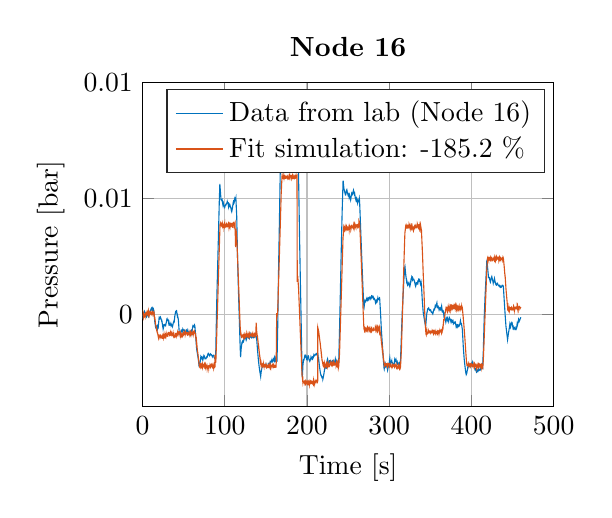
\begin{tikzpicture}

\begin{axis}[%
scaled y ticks = false,
 y tick label style={/pgf/number format/fixed,
/pgf/number format/1000 sep = \thinspace}, % Optional if you want to replace comma as the 1000 separator 
width=2.0556in,
height=1.62135in,
at={(1.011in,0.642in)},
scale only axis,
xmin=0,
xmax=500,
xlabel={Time [s]},
xmajorgrids,
ymin=-0.004,
ymax=0.01,
ylabel={Pressure [bar]},
ymajorgrids,
axis background/.style={fill=white},
title style={font=\bfseries},
title={Node 16},
legend style={legend cell align=left,align=left,draw=white!15!black}
]
\addplot [color=mycolor1,solid]
  table[row sep=crcr]{%
0.05	-0.000213874046920901\\
1.15	1.8413343108814e-05\\
2.2	9.41024926688488e-05\\
2.4	0.000119332209188874\\
3.25	4.53830400781036e-05\\
4.3	-4.422595307918e-05\\
4.85	-0.000113825171065438\\
5.35	-7.11956500489136e-05\\
6.3	-2.6826148582626e-05\\
6.7	-1.8996236558988e-05\\
7.2	-9.12054252195926e-05\\
7.5	-5.29258553273876e-05\\
8.55	6.80027859235183e-05\\
9.6	0.000156741788856316\\
10.65	0.000245480791788544\\
10.75	0.000253310703811821\\
11.5	0.000169791642227829\\
12.15	0.00024896075268728\\
12.55	0.000188931427174369\\
13.1	0.000227210997067101\\
13.85	8.54025904201555e-05\\
14.9	-0.000335672678397209\\
15.9	-0.000565350097751716\\
16.3	-0.000539250391006996\\
16.8	-0.000582749902248408\\
17.5	-0.000517500635386386\\
18.1	-0.000637559286412362\\
19.1	-0.000474871114369904\\
19.25	-0.000500970821114985\\
20.15	-0.000160804643207002\\
20.8	-0.000190384310850819\\
21.25	-0.000113825171065798\\
21.5	-0.000108605229716771\\
22.35	-0.000186904349950751\\
23.35	-0.000307832991202184\\
23.55	-0.000297393108503852\\
24.45	-0.000515760654935457\\
24.55	-0.00050880073313693\\
25.05	-0.000641909237535931\\
25.55	-0.000571440029325229\\
25.9	-0.000467041202345378\\
26.95	-0.000445291446725116\\
27.55	-0.000508800733138262\\
27.95	-0.000511410703812873\\
28.7	-0.000391352052786176\\
29.75	-0.000195604252200207\\
29.8	-0.000192994281525777\\
30.25	-0.000265203470185882\\
31.1	-0.000243453714565897\\
31.85	-0.000401791935484952\\
32.2	-0.000353942473119442\\
32.8	-0.000472261143695391\\
33.15	-0.000480961045943779\\
34	-0.000448771407624823\\
34.35	-0.000409621847506994\\
34.7	-0.000482701026392571\\
35.05	-0.000437461534701131\\
36.1	-0.000510540713586694\\
36.45	-0.000541860361680538\\
37.15	-0.000413971798630217\\
38.15	-0.000303483040076657\\
38.55	-0.000325232795696836\\
39.3	-6.68456989237065e-05\\
40.3	0.000111502297166208\\
41.15	0.000140211974585094\\
41.35	0.000101062414467959\\
41.5	0.000109762316716527\\
42.25	-6.77156891486369e-05\\
42.45	-4.68359237526805e-05\\
43.55	-0.000229533870967399\\
44.6	-0.000778497702834377\\
45.65	-0.000895946383185395\\
45.7	-0.000898556353859825\\
46.7	-0.000762837878785685\\
47.2	-0.000699328592373788\\
48.3	-0.000768057820135601\\
48.85	-0.00069236867057508\\
49	-0.000641039247310737\\
49.9	-0.000695848631474427\\
50.65	-0.00068192878787772\\
50.95	-0.000749788025414255\\
51.9	-0.000839397018571678\\
52	-0.000823737194524762\\
53.05	-0.000721078347995383\\
53.45	-0.000692368670576496\\
54.1	-0.000745438074290686\\
54.4	-0.000761967888562892\\
54.95	-0.000693238660800885\\
55.2	-0.000738478152491978\\
56.25	-0.000846356940369858\\
56.8	-0.000790677565980877\\
57.2	-0.000859406793741288\\
57.75	-0.000892466422283564\\
58.3	-0.000831567106546624\\
58.35	-0.000833307086996471\\
59.15	-0.000746308064513659\\
59.8	-0.00084026700879572\\
60.5	-0.000655829081130252\\
61.25	-0.000500970821113375\\
62.35	-0.000544470332355149\\
62.6	-0.000506190762462944\\
63.1	-0.000462691251221545\\
63.65	-0.000514890664710443\\
64.7	-0.000989035337241997\\
65.8	-0.0015101594819168\\
66.85	-0.00173287697947198\\
67.9	-0.00196951432062707\\
68.7	-0.00222790141740144\\
69.2	-0.00220180171065752\\
70	-0.00208087306940714\\
70.95	-0.00183118587488169\\
71.7	-0.00189382517107009\\
72.15	-0.00184162575757905\\
72.2	-0.00184075576735447\\
73.2	-0.00198343416422733\\
73.25	-0.00198778411535161\\
74.25	-0.00184423572825419\\
74.3	-0.00184771568915354\\
74.65	-0.0017850763929655\\
75.3	-0.00182248597263135\\
75.95	-0.00193384472140894\\
77	-0.00193123475073594\\
77.45	-0.00189382517106688\\
78.1	-0.00184510571847699\\
78.5	-0.00185728558162312\\
79.3	-0.00174505684261742\\
79.55	-0.00175549672531583\\
80	-0.00169807737047807\\
81	-0.00174592683284447\\
81.55	-0.00178507639296124\\
81.7	-0.00175897668621661\\
82.75	-0.00171721715542435\\
83.2	-0.00176332663733876\\
83.95	-0.00175636671554395\\
84.85	-0.00182857590420692\\
84.9	-0.00183553582600526\\
85.2	-0.00180682614858443\\
86.55	-0.00177463651026495\\
87	-0.00186772546432333\\
87.2	-0.0018668554740984\\
87.75	-0.00192079486803787\\
88.75	-0.00193645469208657\\
89.1	-0.00155800894428355\\
90.15	0.000412518914952614\\
91.2	0.00187671246334095\\
92.3	0.0033783155913962\\
93.35	0.00487208880742569\\
94	0.00561680043987989\\
94.4	0.00543932243401454\\
95.4	0.00496082781035871\\
95.5	0.00496430777125842\\
96.5	0.00489731852394681\\
96.85	0.00492863817204171\\
97.6	0.00474159027370324\\
97.9	0.00468417091886476\\
98.35	0.00477551989247293\\
98.65	0.00472071050830924\\
99.7	0.00463893142717599\\
99.95	0.00461022174975623\\
100.75	0.00470070073313911\\
101.65	0.00475464012707894\\
101.8	0.00474333025415523\\
102.85	0.00482771930596433\\
103.05	0.00486077893450731\\
103.55	0.00479813963831856\\
103.95	0.00479900962854314\\
104.55	0.00464415136852414\\
105.05	0.00475290014662766\\
106.05	0.00466242116324585\\
106.35	0.00470157072336297\\
107.1	0.00461109173997938\\
107.35	0.00461283172042923\\
108.05	0.00446319340175695\\
108.45	0.00442317385141526\\
109.25	0.00456759222873619\\
110.3	0.00482075938416206\\
110.4	0.00483467922775913\\
110.75	0.00475986006842352\\
111.35	0.00479987961876593\\
112.25	0.00500084736070218\\
113.2	0.00492863817204563\\
113.45	0.00500693729227952\\
113.5	0.0050147672043028\\
114.55	0.00421350620723471\\
115.6	0.00233345733137892\\
116.65	0.00100411226783767\\
117.7	-0.000235623802543855\\
118.75	-0.00144491021505398\\
119.25	-0.00186076554252249\\
119.85	-0.00152581930596372\\
120.9	-0.00122654266862095\\
121.35	-0.00119000307917683\\
121.6	-0.00123263260019402\\
122.2	-0.00120044296187596\\
122.95	-0.00112910376343971\\
123.05	-0.00114302360703748\\
124	-0.00101339506353748\\
124.05	-0.00101774501466141\\
124.75	-0.0009411858748756\\
125.15	-0.000989905327465498\\
126.05	-0.00112388382208943\\
126.25	-0.00110561402736845\\
127.25	-0.000946405816227291\\
127.45	-0.000929006011731584\\
128.3	-0.000984685386122688\\
128.4	-0.000980335434998758\\
128.65	-0.00101861500489096\\
129.8	-0.00106037453568784\\
130.45	-0.000977725464330018\\
131.05	-0.000877676588475415\\
131.5	-0.000962065640281673\\
132.5	-0.00102992487781679\\
132.55	-0.00102905488759152\\
133.5	-0.000960325659830397\\
134.15	-0.000959455669605827\\
134.45	-0.00101513504399267\\
134.85	-0.00101948499511624\\
135.2	-0.000996865249273102\\
135.75	-0.00100469516129709\\
136.55	-0.000919436119267689\\
136.8	-0.000942055865112243\\
137.85	-0.000976855474109348\\
138.3	-0.000965545601187071\\
138.9	-0.00111083396873045\\
139.95	-0.00159628851418392\\
141.05	-0.0020365035679433\\
142.1	-0.00235231001955259\\
143.15	-0.00258372741935207\\
143.65	-0.00269334618768087\\
144.2	-0.00250542829911853\\
145.25	-0.00231316045943404\\
146.35	-0.00218092194525499\\
146.8	-0.00216004217985886\\
147.4	-0.00222616143694483\\
147.6	-0.00223225136851968\\
148.3	-0.00219049183772883\\
148.45	-0.00220354169110026\\
149.2	-0.00225052116324138\\
150	-0.00216439213098528\\
150.55	-0.00224617121212066\\
151.4	-0.00230620053763675\\
151.8	-0.00229750063538747\\
152.7	-0.00219484178885668\\
152.85	-0.00216004217986242\\
153.7	-0.00219919173998095\\
153.95	-0.00215134227761242\\
154.65	-0.00220180171065397\\
154.8	-0.00219049183773026\\
155.35	-0.00205477336265292\\
155.95	-0.00209044296187247\\
156.9	-0.0020086638807378\\
157.3	-0.00196516436949781\\
157.9	-0.00207565312805118\\
158.05	-0.00207565312804905\\
159.05	-0.00196429437927537\\
159.2	-0.00198082419354721\\
159.85	-0.00191035498533128\\
160.4	-0.00199561402736707\\
161	-0.00183292585532516\\
161.15	-0.00184423572824743\\
162.05	-0.00204781344086202\\
162.25	-0.00204955342131188\\
162.65	-0.00198865410557476\\
163.55	-0.00201127385141649\\
164.35	-0.000661919012707582\\
165.4	0.00188541236558988\\
166.45	0.00397947883675298\\
167.5	0.00621448372434157\\
168.6	0.00847384833821675\\
168.95	0.00881488450635072\\
169.65	0.00853213768328229\\
170.7	0.00810236251221708\\
171	0.00808931265884494\\
171.65	0.00813716212120992\\
171.75	0.00812672223851078\\
172.8	0.00797447394916657\\
173.8	0.0078744250733109\\
174	0.00789443484848175\\
174.95	0.00771434687194199\\
175.3	0.00771173690126685\\
175.7	0.00774044657868768\\
176.4	0.00774392653959023\\
177	0.00768302722385028\\
177.05	0.00769172712609956\\
178.05	0.00782309565004764\\
178.8	0.00784745537634064\\
179	0.00778220610947852\\
179.2	0.00779612595307808\\
179.9	0.00799709369501185\\
180.25	0.00793532438904802\\
181.15	0.00785528528836107\\
181.3	0.00788921490712935\\
181.9	0.00795011422286647\\
182.35	0.00790748470185176\\
183.4	0.00780743582599681\\
184.2	0.00789269486803119\\
184.5	0.00782570562071851\\
185	0.00769085713587143\\
186.1	0.0077561064027378\\
186.6	0.00760124814271845\\
186.9	0.00752990894428433\\
187.65	0.00754730874878147\\
188	0.00746465967742294\\
188.9	0.00752468900293547\\
189.8	0.00587083758553388\\
190.85	0.0035375238025402\\
191.9	0.00152262644183521\\
192.95	-0.000404401906159563\\
194	-0.00246105879765256\\
194.35	-0.00272118587487642\\
195.1	-0.00218788186705797\\
195.75	-0.00198604413489537\\
196.15	-0.00199387404691723\\
197.2	-0.00182074599217545\\
197.3	-0.00180334618767904\\
197.95	-0.00183814579667188\\
198.45	-0.00179464628543473\\
199.1	-0.00188512526881442\\
199.3	-0.001852935630496\\
200.25	-0.00195907443792297\\
200.4	-0.00193558470185311\\
201.35	-0.00179899623656257\\
201.7	-0.00180508616813671\\
202.45	-0.00195733445748163\\
202.55	-0.0019538544965805\\
203.45	-0.00203563357771445\\
203.55	-0.00202519369501604\\
204.6	-0.00191383494623597\\
204.9	-0.00184336573802357\\
206.05	-0.00193297473117655\\
206.55	-0.00187816534701286\\
207	-0.00192688479960242\\
207.8	-0.00186076554251005\\
208.45	-0.00174418685238679\\
208.85	-0.00176506661778079\\
209.35	-0.00179290630497279\\
209.9	-0.00176854657868193\\
210.95	-0.00171721715541866\\
211.55	-0.00174766681328367\\
212.05	-0.00170677727271669\\
213.05	-0.00174418685238538\\
213.2	-0.00173896691103652\\
214.1	-0.00197734423264254\\
214.25	-0.00196255439882054\\
215.2	-0.00226705097751181\\
216.25	-0.00252630806451466\\
217.05	-0.00265158665688932\\
217.35	-0.00264549672531376\\
218.25	-0.00273858567937356\\
219.05	-0.00271161598240328\\
219.3	-0.00280470493645953\\
219.45	-0.00278121520038968\\
220.5	-0.00259764726294665\\
221.4	-0.00237927971651504\\
221.55	-0.00238536964808776\\
222.45	-0.00227488088953083\\
223.5	-0.00232012038121997\\
223.7	-0.00226444100683028\\
224.65	-0.00197299428151186\\
225	-0.00193732468229445\\
225.8	-0.00211828264906092\\
226.4	-0.00218614188659745\\
226.85	-0.00211219271749104\\
227.6	-0.00200779389051464\\
228.6	-0.00199387404691864\\
229	-0.0020678232160279\\
229.9	-0.00212785254154045\\
230.05	-0.00211915263929117\\
231.1	-0.00200866388073495\\
231.3	-0.00200257394916152\\
232	-0.00206347326490007\\
232.35	-0.0020434634897285\\
233.05	-0.00211219271749245\\
233.35	-0.0020982728738929\\
234.3	-0.00197212429129438\\
234.45	-0.00193819467252612\\
234.95	-0.00204172350928504\\
235.45	-0.00199648401759592\\
235.8	-0.00204607346041218\\
236.45	-0.00201649379276818\\
237.35	-0.00214264237536457\\
237.75	-0.00217918196480656\\
238.55	-0.00210175283479759\\
239.6	-0.000654959090903892\\
240.65	0.00103456192571653\\
241.7	0.00282413181818623\\
242.75	0.00439446417399762\\
243.85	0.00572206925708298\\
243.95	0.00576643875854825\\
244.9	0.00542627258063388\\
245.95	0.00526880434993868\\
246.8	0.00514265576734371\\
247.1	0.00514439574779499\\
248.05	0.00534449349950561\\
248.45	0.0053723331866969\\
249.15	0.00524618460409909\\
250.1	0.00512525596285297\\
250.8	0.00517658538611625\\
251.25	0.0050452168621703\\
251.75	0.00512525596285156\\
252.3	0.00502781705766819\\
252.6	0.00503738695014062\\
253.1	0.00493733807428424\\
253.35	0.0049869275170998\\
254.3	0.0052052950635314\\
254.5	0.0051870252688104\\
255.4	0.00523226476050238\\
255.55	0.00520442507330754\\
256.55	0.00534884345062492\\
257.6	0.00517658538611483\\
258	0.0052079050342108\\
258.65	0.00504086691104388\\
258.75	0.00504521686216745\\
259.55	0.0049208082600188\\
260.1	0.00498170757575449\\
260.35	0.00490601842619325\\
260.85	0.00494516798631107\\
261.6	0.00479291969696545\\
261.85	0.00483902917887914\\
262.2	0.00490427844574268\\
262.95	0.00487382878787269\\
263.6	0.00500432732159337\\
263.95	0.00490253846528928\\
265	0.00394032927663088\\
266.1	0.00290330092863582\\
267.15	0.00193935175952543\\
268.2	0.00102934198435134\\
269.25	0.000262880596282836\\
269.3	0.000258530645159252\\
270.3	0.000538667497554685\\
270.55	0.000583906989249497\\
271.4	0.000542147458450132\\
272.45	0.000664816080158184\\
272.8	0.000691785777133427\\
273.45	0.000583036999022804\\
273.75	0.000575207087002358\\
274.55	0.000698745698931427\\
274.6	0.000700485679380566\\
275.35	0.000634366422284649\\
275.6	0.000656116177908186\\
276.55	0.000740505229720842\\
276.8	0.000735285288370566\\
277.6	0.000650896236562185\\
277.75	0.0006648160801596\\
278.7	0.000798794574786377\\
278.95	0.000796184604110531\\
279.35	0.000721365444767461\\
280.25	0.000760515004892395\\
280.7	0.000692655767344494\\
280.9	0.000717885483869168\\
281.55	0.000662206109485169\\
282	0.000670906011735153\\
283.05	0.000553457331380236\\
283.4	0.000488208064519546\\
284.1	0.000571727126114016\\
284.2	0.000586516959936723\\
284.95	0.000508217839698205\\
285.2	0.00052213768329136\\
286.15	0.000697875708707565\\
286.2	0.000690045796682859\\
286.8	0.000631756451608803\\
287.65	0.000656116177905355\\
288.25	0.000707445601170045\\
288.35	0.000703095650045046\\
289.4	8.19226295099701e-05\\
290.45	-0.00067496886608398\\
291.5	-0.00122654266862202\\
292.6	-0.00180682614857448\\
293.65	-0.00231490043986685\\
293.95	-0.00236622986313011\\
294.7	-0.00219136182794488\\
295.15	-0.00213307248287793\\
295.75	-0.00223747130986356\\
296	-0.002203541691096\\
296.8	-0.00226357101661211\\
297.1	-0.00226009105571523\\
297.9	-0.00238101969697271\\
298.05	-0.0024149493157417\\
298.95	-0.00226183103617432\\
299	-0.00226357101662204\\
300	-0.00210436280547202\\
300.75	-0.00190078509285388\\
301.05	-0.00200779389050683\\
301.75	-0.00215830219940261\\
302.1	-0.00210175283479049\\
303.05	-0.00200518391982672\\
303.2	-0.00205303338218886\\
304.2	-0.00211915263928052\\
304.25	-0.00211741265882995\\
305.3	-0.00222703142715733\\
305.8	-0.00224617121210502\\
306.35	-0.00207826309870927\\
306.75	-0.0019538544965606\\
307.4	-0.002022583724321\\
308.2	-0.00195211451611714\\
308.45	-0.00200779389050541\\
309.15	-0.00209044296186607\\
309.7	-0.00205564335287607\\
310.2	-0.00215308225805802\\
310.95	-0.00212263260019444\\
311.65	-0.00219571177907414\\
311.7	-0.00219832174974714\\
312.35	-0.00212872253176147\\
312.9	-0.00220528167153804\\
313.75	-0.00200605391005484\\
314.85	-0.000898556353856633\\
315.9	9.67124633497185e-05\\
316.95	0.000850993988270668\\
318	0.00158961568915214\\
319.05	0.00205245048877242\\
319.15	0.00206289037147013\\
320.15	0.00168531461391479\\
321.2	0.00140604775173966\\
321.45	0.00143823739005951\\
322.25	0.00130425889543984\\
322.45	0.0012572794232973\\
323.3	0.00131643875858242\\
323.85	0.00135558831869173\\
324.35	0.00125640943306064\\
325.05	0.00118768020530309\\
325.45	0.00124683954059675\\
326.35	0.00144867727275295\\
326.5	0.00143040747803054\\
327.45	0.00161658538614728\\
327.55	0.00160875547412399\\
328.3	0.00149739672534747\\
328.65	0.00155916603131556\\
329.4	0.00148956681332846\\
330	0.00149739672534463\\
330.75	0.00141039770285756\\
331.8	0.00123291969699364\\
332.15	0.0011981200880008\\
332.75	0.00130686886610432\\
332.95	0.00128772908115804\\
333.4	0.00133731852396506\\
333.95	0.00131382878789378\\
334.55	0.00138690796677776\\
334.95	0.00134253846531249\\
335.85	0.00150696661780285\\
336.1	0.00149826671555287\\
336.65	0.00144519731184187\\
337.1	0.00147477697948302\\
338.15	0.00126510933530495\\
338.45	0.00124422956991237\\
338.9	0.00134601842621788\\
339.2	0.00127293924732964\\
340.25	0.000576947067469982\\
341.35	7.32227272969288e-05\\
342.4	-0.000159934652973731\\
343.45	-0.00037569222874867\\
344.25	-0.000530550488773707\\
344.5	-0.000481831036182032\\
345.55	-6.81637343194486e-06\\
346.65	0.000194151368507506\\
346.75	0.000188931427158659\\
347.65	0.000251570723349179\\
347.95	0.000267230547395747\\
348.75	0.000201111290315456\\
349.1	0.000161961730196197\\
350.35	0.000186321456501284\\
350.85	0.000105412365591182\\
351.1	0.000108022336261351\\
351.4	7.75726783892317e-05\\
351.95	8.45326001815555e-05\\
353	9.71344085411163e-06\\
354.05	0.00016370171064535\\
354.4	0.000211551173007488\\
355.15	0.00019154139782597\\
356	0.000367279423253541\\
356.7	0.000319429960887144\\
357.25	0.000389899169095265\\
358	0.000489078054726352\\
358.3	0.000390769159317697\\
358.75	0.000292460263910471\\
359.55	0.000331609824031145\\
360.4	0.000228950977498935\\
360.65	0.000186321456479968\\
361.45	0.000280280400766456\\
361.5	0.000282020381215609\\
362.25	0.000188931427158659\\
362.65	0.000173271603110661\\
363.6	0.000321169941334867\\
363.75	0.000346399657855281\\
364.6	0.000104542375354524\\
364.65	0.000106282355803677\\
365.55	0.000148041886591677\\
365.7	0.000139341984344524\\
366.45	-6.16257576048634e-05\\
366.95	2.75351903479548e-06\\
367.7	-0.000166024584586241\\
367.8	-0.000166024584584812\\
368.85	-0.000350462512248156\\
368.9	-0.000342632600224865\\
369.95	-0.00016776456503112\\
370.25	-0.000143404838733138\\
370.9	-0.000250413636387517\\
371.2	-0.000205174144691275\\
372.05	-0.000292173167162721\\
372.25	-0.000318272873908426\\
373.1	-0.000146014809387682\\
374.2	-0.000236493792775891\\
374.35	-0.000233883822098616\\
375.25	-0.000353072482904102\\
376	-0.000249543646145184\\
376.45	-0.00026868343109572\\
376.85	-0.000323492815257273\\
377.55	-0.000285213245368995\\
378.1	-0.00042006173021536\\
378.4	-0.000405271896395498\\
379.35	-0.000353942473133653\\
379.8	-0.000380912170107481\\
380.35	-0.000348722531790482\\
380.55	-0.000374822238537603\\
381.5	-0.000565350097770811\\
381.7	-0.000551430254177657\\
382.35	-0.000487920967764691\\
382.85	-0.000545340322603519\\
383.35	-0.000484441006867828\\
384.05	-0.000529680498555535\\
384.8	-0.000471391153487155\\
385.35	-0.000495750879780862\\
385.85	-0.000437461534715342\\
386.65	-0.000284343255140859\\
386.9	-0.000340022629523443\\
387.55	-0.000431371603132669\\
387.95	-0.000426151661779547\\
389	-0.000676708846528859\\
390.1	-0.00141707052785381\\
391.15	-0.00191905488757629\\
392.2	-0.0022687909579638\\
393.15	-0.00252804804495173\\
393.4	-0.00251673817202873\\
393.75	-0.00260373719450871\\
394.3	-0.00256023768327014\\
395.4	-0.00234361011727986\\
395.8	-0.00222355146625619\\
396.95	-0.00226531099704419\\
397.5	-0.00223573132940162\\
398.05	-0.00218005195501336\\
398.55	-0.00226270102637119\\
398.6	-0.0022661809872709\\
399.55	-0.00216265215052192\\
400.1	-0.00212959252197538\\
400.55	-0.00219310180838693\\
400.7	-0.00218092194523865\\
401.2	-0.00207739310848257\\
401.95	-0.00215656221893641\\
402.8	-0.00224878118276808\\
403.55	-0.00223312135872578\\
403.85	-0.00229837062558505\\
404.4	-0.00239754951121045\\
404.95	-0.00237840972626417\\
406	-0.00249237844572081\\
406.1	-0.00250020835774693\\
406.85	-0.00242799916908683\\
407.65	-0.00247323866078449\\
408.1	-0.00240885938415192\\
408.4	-0.0023549199902128\\
408.8	-0.00241581930595418\\
409.15	-0.00239319956010678\\
410	-0.00242016925707776\\
410.2	-0.00239841950145421\\
411.25	-0.00231490043987252\\
411.5	-0.00236709985336107\\
412.35	-0.00229750063537966\\
412.8	-0.00227314090908026\\
413.3	-0.00232708030301512\\
413.55	-0.00233752018570998\\
414.45	-0.00159280855326005\\
415.5	-0.000203434164212299\\
416.55	0.000738765249271703\\
417.65	0.00152871637342213\\
418.7	0.00229430777127886\\
418.85	0.00235259711634581\\
419.75	0.00197328137832427\\
420.8	0.00158352575760785\\
421.45	0.00158526573805841\\
421.8	0.00154872614861216\\
421.9	0.00155220610950903\\
422.95	0.00138342800588799\\
423.1	0.00137385811341414\\
424	0.00155046612904426\\
424.75	0.00161919535681602\\
425.05	0.00156786593355275\\
426.1	0.00141039770284902\\
426.5	0.00133296857284149\\
426.95	0.00141474765397402\\
427.35	0.00140169780060188\\
428	0.00153741627567495\\
428.25	0.00149652673511082\\
429.3	0.00131643875857106\\
430.25	0.00125031950148935\\
430.5	0.00124683954058821\\
431.35	0.00134166847509573\\
431.55	0.00134079848487187\\
432.45	0.00126162937441802\\
433.45	0.00121551989249366\\
433.9	0.00123204970676551\\
434.1	0.0012007300586738\\
434.6	0.00122682976541523\\
435.55	0.00115027062563013\\
436.2	0.00115288059630882\\
436.45	0.00119812008799937\\
436.8	0.00119290014665194\\
437.45	0.00124683954059247\\
438.35	0.0012424895894817\\
438.85	0.00117637033239856\\
439.9	0.000579557038165715\\
440.95	-4.20640270493156e-06\\
442	-0.000529680498511473\\
443.05	-0.000834177077214115\\
443.95	-0.00110300405669864\\
444.15	-0.00104993465298338\\
445.2	-0.000787197605084375\\
446.25	-0.000561000146630186\\
446.75	-0.000428761632449717\\
447.6	-0.000557520185721957\\
448.35	-0.000431371603128408\\
448.6	-0.000377432209186443\\
449.4	-0.000437461534696856\\
449.65	-0.000413101808403149\\
450.5	-0.000590579814267064\\
450.9	-0.000556650195500927\\
451.55	-0.000662789002941394\\
451.6	-0.000664528983390533\\
452.6	-0.000575789980464259\\
453	-0.000561870136868259\\
453.65	-0.000666268963851052\\
454.05	-0.000672358895422345\\
454.4	-0.000636689296205639\\
454.75	-0.000636689296207069\\
455.6	-0.000420061730229571\\
455.95	-0.00047574110461783\\
456.85	-0.000349592522010084\\
457.35	-0.000230403861208858\\
458.1	-0.000312182942337133\\
458.85	-0.000248673655929843\\
460	-0.000136444916932307\\
};
\addlegendentry{Data from lab (Node 16)};

\addplot [color=mycolor2,solid]
  table[row sep=crcr]{%
0.05	0.000193223171070573\\
1.05	-0.000117811203972184\\
1.15	-9.50145980933565e-05\\
1.35	1.50434389271251e-05\\
2.4	-0.00010029515911943\\
3.2	1.87516450794827e-05\\
3.9	5.11544310798235e-05\\
4	-5.09741258605396e-05\\
4.45	2.59328486432396e-05\\
4.7	-4.01074833832405e-05\\
5.6	-2.46337562505425e-05\\
6	7.70923488628309e-05\\
6.8	-3.28771826403553e-05\\
7.25	9.48977364217567e-05\\
7.5	-1.35778890175342e-05\\
8.25	6.43027608677842e-05\\
8.7	-3.3954183465429e-05\\
9.1	5.09838655413434e-05\\
9.7	9.70060214108758e-05\\
10.65	2.05480353292689e-05\\
11.25	-2.15551280110551e-05\\
11.6	6.91583415908329e-05\\
11.85	3.94901335122597e-06\\
12.5	9.41805823802161e-05\\
13.35	7.61207193625353e-05\\
13.6	1.14556220916275e-05\\
14	6.17055586469667e-05\\
14.7	-0.00017431169115607\\
14.9	-0.000163624496884102\\
15.95	-0.000454405691143786\\
17.05	-0.000667051340543739\\
17.2	-0.00064259520528025\\
18.1	-0.000814060092264464\\
18.25	-0.000807581804150953\\
19.15	-0.000987243393604689\\
19.55	-0.00104192593395218\\
20.15	-0.000880117499145202\\
20.2	-0.000915724474088942\\
21.25	-0.000995799893068183\\
21.3	-0.00100363374766236\\
22.1	-0.000907310906970963\\
22.4	-0.000921004913981383\\
22.8	-0.00102724044967806\\
24.05	-0.00103956494843388\\
24.3	-0.000936038096017233\\
24.65	-0.00090020271899027\\
25.3	-0.00103406066100047\\
26.1	-0.000881616886326229\\
26.45	-0.00100132832195336\\
27.05	-0.00102501198542517\\
27.65	-0.000868514050273426\\
27.7	-0.000865523635612269\\
28.4	-0.000966780336942486\\
28.8	-0.000850267222629511\\
29.3	-0.000949057391283637\\
30.4	-0.000953786039271969\\
30.8	-0.00080549101275556\\
31.05	-0.00090561731039925\\
31.4	-0.000790589165104579\\
32.4	-0.000789348338830589\\
32.7	-0.00092818063249228\\
33.8	-0.000904973024901168\\
34	-0.000807815399316736\\
34.15	-0.000777662048581549\\
34.8	-0.000874083157055596\\
35.15	-0.000815230678743447\\
35.85	-0.000913010934474416\\
36.35	-0.000922361489725022\\
37.05	-0.0008132867461849\\
37.15	-0.0008475258799088\\
37.6	-0.000946486523927056\\
38.25	-0.000867485465967376\\
39.15	-0.00100090489794932\\
40.1	-0.000971105483747924\\
40.25	-0.000886466443968893\\
40.7	-0.000918993574103662\\
41.4	-0.000822511258776856\\
41.45	-0.000808385462566382\\
41.65	-0.000918123105739251\\
42.7	-0.000764299923742979\\
43.3	-0.000887716158095976\\
43.7	-0.000836608780792269\\
44.2	-0.0007636727292611\\
44.85	-0.000758642565263595\\
45.45	-0.000883732558228424\\
45.8	-0.000807542195090265\\
46.45	-0.000943175615381996\\
46.7	-0.000878387200988526\\
47.25	-0.000953191623658352\\
47.95	-0.000874235513749884\\
48.65	-0.00095778657092015\\
48.95	-0.000927579887651325\\
49.55	-0.000807963303060932\\
49.9	-0.000885109975376638\\
50.95	-0.000806494314567593\\
51.35	-0.000852540734097206\\
51.95	-0.000779610278567726\\
52.05	-0.000851055316305872\\
52.5	-0.000774060961147312\\
53.4	-0.00078746238200154\\
54.05	-0.000878691921855075\\
54.55	-0.000898506646074975\\
54.85	-0.000803348929922583\\
55.55	-0.000814447979085411\\
56	-0.000886973319397188\\
56.35	-0.000880320579872691\\
56.7	-0.000786600736306769\\
57.5	-0.00091161062367246\\
58.1	-0.000813619022735596\\
58.5	-0.000866236702557294\\
58.65	-0.000744254868415675\\
59.55	-0.00079887830911363\\
59.85	-0.000884458348273408\\
60.75	-0.000875289870011977\\
61.1	-0.000783117344781311\\
61.65	-0.000900642014614959\\
62.35	-0.000778123065122765\\
62.75	-0.000795290228559245\\
63.15	-0.00073501098611056\\
63.7	-0.000783187200849741\\
64.55	-0.000953061087508591\\
64.7	-0.000936636351583679\\
65.6	-0.00126420623565495\\
65.8	-0.00121192507082874\\
66.8	-0.00160898276007833\\
66.85	-0.00157724980500837\\
67.9	-0.00188420812372223\\
68.95	-0.00222543783206288\\
69.05	-0.00218486036364293\\
69.45	-0.00228183397981206\\
70.1	-0.00231771947681279\\
70.6	-0.00218512171539531\\
71.4	-0.00226657683829982\\
71.75	-0.00218678373162551\\
72.8	-0.00230651051754107\\
73.05	-0.00214787221000571\\
73.2	-0.00216377126351002\\
74.25	-0.00226314839372845\\
74.65	-0.00228786836544895\\
74.9	-0.0021745208472783\\
75.5	-0.00212811177453955\\
76.3	-0.00230296382506963\\
76.8	-0.00220826486721778\\
77.1	-0.00229995342866807\\
78.3	-0.00221287855815075\\
78.5	-0.00229804539234116\\
78.65	-0.00236538866654188\\
79.35	-0.00224039834230993\\
80.1	-0.00223126840284289\\
80.5	-0.0023473779281086\\
80.7	-0.00228390424086729\\
81.6	-0.00222076986223013\\
81.8	-0.0023060383677569\\
82.1	-0.00220726298388761\\
82.75	-0.00228725908943021\\
83.65	-0.00217278604067564\\
83.95	-0.00219821078250116\\
84.65	-0.0022690913176602\\
84.95	-0.0021990636997407\\
85.9	-0.00229678800960537\\
86.35	-0.0022310055732348\\
86.6	-0.00232268992988604\\
87.05	-0.00223079491612224\\
87.35	-0.00230583676349958\\
88.1	-0.00227525382861958\\
88.15	-0.001758565883497\\
89.1	-0.0020983053827393\\
90.15	-0.000996523275909115\\
91.2	0.000267412680950903\\
92.3	0.00157942403585854\\
93.35	0.00284404703856265\\
94.25	0.00386166859913867\\
94.7	0.00391026022780325\\
94.9	0.00383307252249057\\
95.8	0.00389198335921441\\
96.4	0.00378394093391852\\
97	0.00376779382811484\\
97.2	0.00391124091486361\\
97.6	0.00385467935383054\\
97.8	0.00376927846296685\\
98.95	0.00386887757996082\\
99.1	0.00374627860186069\\
99.95	0.00390683946887927\\
100.15	0.00374268485401099\\
101.55	0.00378310008795386\\
101.8	0.00387313148720449\\
102.05	0.00389253477710145\\
102.4	0.0037662119988675\\
103.15	0.00376594307835215\\
103.7	0.00387548972505245\\
104.35	0.00392740551517802\\
104.95	0.00376064166283896\\
105	0.0037805414119955\\
105.45	0.00386982811811405\\
106.3	0.00375138964233654\\
106.7	0.00388001204014978\\
107.2	0.00382953334718186\\
107.75	0.00391614001148793\\
108.25	0.00391795166203278\\
108.65	0.00377663994090019\\
109.4	0.00375695904441147\\
109.75	0.00392373567995708\\
110.7	0.00395369043599082\\
111.1	0.00385340565040188\\
111.35	0.00394076839191895\\
111.65	0.00381290741151364\\
112.45	0.00392208683089195\\
113.15	0.0028956068081674\\
113.65	0.00368770982486212\\
114.55	0.00331202598823873\\
115.6	0.0023983098122252\\
116.65	0.00144638092627678\\
117.7	0.000434405971451266\\
118.75	-0.000539915344534861\\
119.6	-0.000944822452013172\\
119.85	-0.000870523996859367\\
120.5	-0.00100228881010727\\
121.15	-0.000980854636843282\\
121.3	-0.00090231811091593\\
122.5	-0.00089341584364348\\
122.7	-0.000974529710274652\\
123.2	-0.000904493192499217\\
123.85	-0.0010281831333316\\
124.5	-0.000972231907462135\\
124.65	-0.000885746911404122\\
125.6	-0.00098317891883423\\
126.1	-0.000873876165087928\\
126.3	-0.00097570240007537\\
126.6	-0.00087361970685326\\
127.5	-0.000963135365641693\\
128.3	-0.00084114211402627\\
129	-0.000957905860175207\\
130.05	-0.000846336410669891\\
130.25	-0.000933533204987954\\
130.6	-0.000860565481074724\\
131.1	-0.000941857974798967\\
131.85	-0.000934974897126363\\
132.35	-0.000871032525391415\\
133.15	-0.000953181925216702\\
133.45	-0.000898262552112965\\
133.95	-0.000836795696152463\\
134.35	-0.000955361506480548\\
135.05	-0.000943945105397682\\
135.7	-0.000859303028991326\\
135.8	-0.000851142542679846\\
136.35	-0.000936824797854564\\
137.1	-0.000862216517311802\\
137.35	-0.000938701870413997\\
137.85	-0.000887558419470818\\
138.15	-0.000363735991512833\\
138.9	-0.000771957995661243\\
139.95	-0.00105842995395509\\
140.05	-0.00104417683302519\\
140.95	-0.0013501673044301\\
141.05	-0.00131392071397369\\
142.1	-0.00168978365312665\\
143.05	-0.00197996725022659\\
143.15	-0.0019523499716354\\
144.2	-0.0022150093784133\\
144.4	-0.00214609356509865\\
144.75	-0.0022269324310299\\
145.8	-0.00216530159452701\\
146.15	-0.0022802064502265\\
147.05	-0.00226854704988667\\
147.15	-0.00216519849388837\\
147.75	-0.00227273959996154\\
148.05	-0.00217285829532894\\
148.75	-0.00217482543905603\\
149.35	-0.00226813637529339\\
150.1	-0.00224407971715532\\
150.4	-0.00217432702183322\\
150.7	-0.00220640834709038\\
150.85	-0.00232059795050458\\
152.15	-0.00228174248495452\\
152.3	-0.00222200176208171\\
152.75	-0.00220156743723208\\
153.05	-0.00230941067023279\\
154	-0.00230692895607248\\
154.25	-0.00219334118503182\\
155.1	-0.00231698078573479\\
155.8	-0.00220567895544705\\
156.15	-0.00229265041362172\\
156.45	-0.00221899128900735\\
157.3	-0.00226120815369229\\
158	-0.0021928112709986\\
158.7	-0.00228380689174797\\
159.3	-0.0022018598309451\\
159.85	-0.00229665091202195\\
160.75	-0.00229665605350378\\
160.9	-0.00220856233282704\\
161.15	-0.00220999407353676\\
161.55	-0.00229292442009543\\
162.5	-0.00228485884322995\\
163.15	3.88172292030121e-05\\
163.45	-0.00012669496159768\\
164.35	8.11394001439445e-05\\
165.4	0.00132039592044671\\
166.45	0.0025274366939632\\
167.5	0.00380338318811107\\
168.6	0.00517153453462745\\
169.65	0.00596621746998642\\
169.75	0.0059928375966414\\
170.3	0.0058737987381897\\
171.15	0.00585188016995487\\
171.75	0.00599187972597023\\
172.15	0.00587199535629251\\
172.8	0.00599240502586867\\
172.85	0.00600864394492143\\
173.2	0.00585708612058994\\
174	0.0058649168661675\\
174.55	0.0059327080533356\\
175.9	0.00585641982540443\\
176	0.00595326700142694\\
176.05	0.00596047697590996\\
176.95	0.00588400910716263\\
177.35	0.00585610479020978\\
178.05	0.00596628058966129\\
178.45	0.00590897832440232\\
179	0.00600011787286828\\
179.45	0.00587638761941076\\
180.2	0.00598638567506339\\
180.9	0.00598894110149885\\
181.3	0.00587676628813059\\
181.45	0.00584687354620078\\
182.35	0.00598749715304794\\
183.05	0.00585520226895431\\
183.7	0.00585484549285696\\
184.3	0.00598433240189927\\
184.85	0.00595508158420884\\
185.2	0.00588559172032305\\
186.45	0.00599724854640989\\
186.55	0.00588927149403689\\
187.1	0.00590546328864484\\
187.6	0.00597804460534886\\
187.85	0.0059875928655746\\
188.15	0.00138833671745127\\
188.75	0.00164489065154116\\
189.8	0.00107779314149226\\
190.85	0.000149732537370507\\
191.9	-0.000819971885113833\\
192.95	-0.00171446961555508\\
194	-0.00263620902987721\\
195	-0.00295255387158047\\
195.15	-0.00291566549629344\\
195.25	-0.00297491844478564\\
197.05	-0.00289533695748439\\
197.15	-0.00298286791002152\\
197.4	-0.00301312115856839\\
198.05	-0.00290883719441431\\
198.55	-0.0030000349198558\\
199.2	-0.0029269302057863\\
199.7	-0.00289809936969032\\
200.2	-0.00300701422321979\\
200.7	-0.00303496790070082\\
201.25	-0.00293151437284583\\
201.75	-0.00298928935498869\\
202.4	-0.00290924407117608\\
202.9	-0.00304748544089956\\
203.3	-0.00293522736092965\\
203.7	-0.00291027508382208\\
203.8	-0.00300536115459731\\
204.65	-0.0030042428981613\\
205.25	-0.0028881796975124\\
205.85	-0.0028960037946048\\
206.25	-0.00299594077396852\\
207.15	-0.00302201404026104\\
207.8	-0.00286881200825451\\
208.15	-0.00303036939211705\\
209.45	-0.0029005767795128\\
209.55	-0.00296296993158065\\
209.95	-0.0028680351300052\\
210.85	-0.00294451149179179\\
211.05	-0.00295299532428954\\
212	-0.00285134643970842\\
212.15	-0.00284237145653425\\
212.75	-0.00292461775301658\\
213.1	-0.00288495554928976\\
213.15	-0.000575852274903659\\
214.25	-0.000754856697112642\\
215.2	-0.00102332004683629\\
216.2	-0.00131057799169674\\
216.25	-0.0013061870088663\\
217.35	-0.0016968384437804\\
217.45	-0.00168049992214377\\
218.4	-0.00202519468830272\\
218.45	-0.00199848934703395\\
219.4	-0.00218141166768206\\
220.05	-0.00213240582733794\\
220.3	-0.00226031924324907\\
220.8	-0.0022919666730373\\
221.45	-0.00211754821549625\\
221.55	-0.0021388703849427\\
222.2	-0.00227191272882602\\
223.35	-0.00215371567251881\\
223.5	-0.00224957274693431\\
224.2	-0.00229357689905657\\
224.5	-0.00218823161625754\\
224.85	-0.00227020007346714\\
225.75	-0.00211424744816202\\
225.8	-0.00213034920855895\\
226.45	-0.0022787926330084\\
226.85	-0.00227766760191988\\
227.9	-0.00214056912500342\\
228	-0.00219516533501662\\
228.85	-0.00213102790219003\\
229.55	-0.00218060631317528\\
229.65	-0.00209390804153952\\
230.8	-0.00219870446321217\\
231.05	-0.00211982407534065\\
231.85	-0.00204149991340375\\
232.15	-0.00216615821256768\\
233	-0.0021059639697563\\
233.2	-0.00220239235524951\\
233.7	-0.00219560649827005\\
234	-0.0021223233764628\\
235.1	-0.00211250797927655\\
235.3	-0.00219777478904296\\
235.7	-0.00211252244075\\
236.2	-0.00218823776295424\\
236.45	-0.00212691899664979\\
236.85	-0.00221118869517231\\
237.65	-0.00209431642175903\\
238.15	-0.00232661692022683\\
238.6	-0.00224714309078211\\
239.6	-0.00170067347856559\\
240.65	-0.000460394936355882\\
241.7	0.000746858622166287\\
242.75	0.00203429258102636\\
243.8	0.00327345355210708\\
243.85	0.00327202662726736\\
244.75	0.00375961380218121\\
245.65	0.00364664461201385\\
245.95	0.00375692858675733\\
246.35	0.00380318974347877\\
247	0.00366295117131985\\
247.3	0.00362935673068162\\
248.05	0.00375041831407416\\
248.1	0.00376374007623094\\
248.55	0.00368680439023833\\
249.3	0.00373429331146015\\
249.6	0.00363839068933776\\
250.2	0.00366259219092644\\
251	0.00378371362640502\\
251.35	0.00364100802766612\\
251.95	0.00382472943441905\\
253.05	0.0037837390080614\\
253.35	0.00364477934616352\\
254.45	0.00381841912853622\\
254.5	0.00385708654034102\\
254.9	0.00375221997180013\\
255.95	0.00371502432840887\\
256.55	0.00382672519423278\\
256.7	0.00375713425409526\\
257.4	0.00387723510992399\\
258.05	0.00373060564633001\\
258.55	0.0038599860782837\\
259.5	0.00374973887452399\\
259.65	0.00386116934171874\\
259.8	0.0037385443104396\\
260.05	0.00385039626515933\\
261.3	0.00386480619681534\\
261.5	0.00377749769611825\\
262.3	0.00384910670750537\\
262.65	0.00376024446989986\\
263.1	0.00378364914281134\\
263.15	0.00404301547635509\\
263.95	0.00397753319205884\\
265	0.00320417929768547\\
266.1	0.00220402232885434\\
267.15	0.00124200914707517\\
268.2	0.000231053673067255\\
269.2	-0.000614186547891564\\
269.5	-0.000653904230510054\\
269.65	-0.000549447344347647\\
270.75	-0.000632775459119349\\
270.95	-0.000704480573560038\\
271.55	-0.000628111466704931\\
272.3	-0.00071104187361947\\
272.45	-0.000692617131249408\\
273.2	-0.00059052499468149\\
273.6	-0.000680452136282328\\
274.2	-0.000581406940390045\\
274.85	-0.000641051248316595\\
275.55	-0.000742186797898506\\
275.6	-0.000738289479902789\\
275.95	-0.000609387576188318\\
277.15	-0.000729093671309224\\
277.6	-0.000650608505723362\\
278	-0.000730017023463043\\
278.6	-0.000644964713604559\\
278.95	-0.000734973248552193\\
279.85	-0.000682144532387218\\
280.45	-0.000701136146326129\\
280.65	-0.000603239371836333\\
280.9	-0.000614451802719771\\
281.2	-0.00069683673849152\\
282.7	-0.000682505706578179\\
283	-0.000593386964318773\\
283.6	-0.000691210970892242\\
284.1	-0.000602157869260837\\
284.15	-0.000582366951767273\\
285.05	-0.000719727361503375\\
285.4	-0.000595184635943753\\
285.85	-0.00067957491216216\\
286.2	-0.000606763324870282\\
286.55	-0.000688172662528059\\
287.7	-0.000553225670175431\\
288.15	-0.000754433123138017\\
288.7	-0.000656717184101402\\
289.15	-0.000846511032098964\\
289.5	-0.000830314154488396\\
290.4	-0.0011629808301165\\
290.45	-0.00115597146320915\\
291.35	-0.00146708960209717\\
291.5	-0.00141680189779628\\
292.5	-0.00178638148038579\\
292.6	-0.00176210004177916\\
293.65	-0.00210893513369674\\
293.75	-0.00207260717068606\\
294.5	-0.0022350080056652\\
295	-0.00220573371215702\\
295.3	-0.00213199107059439\\
296.3	-0.00213534109724485\\
296.55	-0.0022201411802265\\
297.45	-0.00214942869866774\\
297.9	-0.00222594182695413\\
298	-0.00225024501587043\\
298.65	-0.0021452953636453\\
299.45	-0.00213708763930779\\
299.9	-0.00224416472764362\\
300.3	-0.00227348318303517\\
301.05	-0.00217126162522415\\
301.1	-0.00216299871610256\\
301.95	-0.00227625799238279\\
302.8	-0.00229165475017411\\
303.15	-0.00221113018024911\\
303.3	-0.00219467818172861\\
303.6	-0.00231123330550932\\
304.25	-0.00226842897808181\\
304.85	-0.00218042930753399\\
305.4	-0.00219062749628814\\
306.35	-0.00227487781789331\\
306.4	-0.00228074153427967\\
307.05	-0.00218263859860288\\
307.5	-0.00221410337536386\\
308.3	-0.00227963772493782\\
308.55	-0.00220892987520958\\
309	-0.00230798851787116\\
309.65	-0.0022380399947552\\
310.45	-0.0023451504025852\\
311.25	-0.00229652942985749\\
311.4	-0.00222334973104155\\
312.2	-0.00232713692031943\\
312.4	-0.00226443089050872\\
312.9	-0.00221598653875951\\
313.4	-0.00232962765982559\\
313.75	-0.00229033552153622\\
314.85	-0.00151539275763319\\
315.9	-0.000224492172273021\\
316.95	0.00105982239891407\\
318	0.00232122414687255\\
319.05	0.00349064108242663\\
320.15	0.00382437200807732\\
320.4	0.00384804384144167\\
321	0.00372905913423733\\
321.25	0.0037387080410869\\
321.75	0.00383698291662404\\
322.4	0.00384172181703196\\
322.75	0.00371303813231381\\
323.9	0.00372889814904226\\
324.2	0.00388907388904329\\
324.6	0.00384983238569822\\
325.35	0.00370623410133062\\
326.15	0.0038087937373104\\
326.45	0.00370114481569497\\
327	0.00379646598808608\\
327.3	0.00372668233197866\\
327.85	0.0037998631708402\\
328.25	0.00370343069403556\\
329.25	0.00361215195828245\\
329.4	0.00378606104718231\\
329.65	0.00368568698704567\\
330.65	0.00379169279642348\\
331.15	0.00371361100217362\\
331.8	0.00379125691974864\\
332.15	0.00382295563400128\\
332.45	0.00373366203037836\\
333.65	0.0037254419199566\\
333.85	0.00381536238155138\\
334	0.00375152275091265\\
334.2	0.00389844099977792\\
335.45	0.00374884848977153\\
335.8	0.00385510137061133\\
336.55	0.00386217221751769\\
336.75	0.00374851228774635\\
337.25	0.00385125988505105\\
337.7	0.00370375048117541\\
338.15	0.00383337423031374\\
339.15	0.0036224384207088\\
339.2	0.0036343174843225\\
340.25	0.00277136541346048\\
340.3	0.00277708692670265\\
341.35	0.00174929746658473\\
342.4	0.00083885303795098\\
343.45	-0.000154820747240437\\
344.5	-0.000763306478700117\\
344.9	-0.000705448778488288\\
345.5	-0.000848192726503919\\
345.85	-0.000758818225663615\\
346.1	-0.000862625165458804\\
347.05	-0.000831879501035407\\
347.7	-0.000747193265955415\\
347.8	-0.000824713824915679\\
348	-0.000722387639000761\\
349.55	-0.000727671593611565\\
349.7	-0.000823902688580291\\
349.9	-0.000832949094980498\\
350.5	-0.000742094661465275\\
351.1	-0.000737222227894651\\
351.2	-0.000808818748309884\\
352.1	-0.000800519024380867\\
352.3	-0.000720215276963086\\
353.3	-0.000809642066379888\\
353.7	-0.000709402464851171\\
354.2	-0.000727353881766487\\
354.3	-0.000826444421874347\\
355.15	-0.000739946438635345\\
356	-0.00084334380956361\\
356.6	-0.000751427215865105\\
356.95	-0.000841859848450976\\
357.3	-0.000835340597461806\\
358.3	-0.000748027955433719\\
358.55	-0.000735680447896924\\
358.7	-0.000868437295211351\\
359.5	-0.000827122066836052\\
360.25	-0.000724635351919331\\
360.7	-0.000741474569409782\\
360.8	-0.000823813211237686\\
361.5	-0.000703132148141265\\
361.85	-0.000763600730488796\\
362.9	-0.000701514362689628\\
363.6	-0.000817010128102686\\
364.5	-0.000668314512814148\\
364.65	-0.000696843655800078\\
365.65	-0.000466300485622779\\
365.7	-0.000480634071552177\\
366.25	-0.000254243770603472\\
366.75	-0.000262374907952466\\
367.8	-6.70893370802662e-06\\
368.9	0.000228537054023333\\
369.1	0.000204304741256247\\
369.35	0.00029869432994996\\
370.45	0.000278550798049678\\
370.85	0.000164458385481493\\
371.45	0.000284069614814892\\
371.65	0.000176654309567186\\
372.4	0.000289374962344146\\
373.1	0.000206903517456678\\
373.15	0.000193987123876135\\
373.75	0.000317514245933236\\
374.3	0.000190273771441583\\
374.7	0.000333749454852495\\
375.5	0.000242361359425226\\
375.85	0.000391352372629804\\
376.65	0.000375429537750732\\
377.1	0.0002612682624232\\
377.8	0.00034950767359607\\
378.35	0.000234542368664248\\
378.45	0.000236035087319673\\
379.35	0.000364114753846465\\
380.1	0.000241982381146966\\
380.45	0.000348548014788401\\
380.65	0.000387735156268433\\
381.25	0.000279181501062399\\
381.8	0.000203289543952511\\
381.95	0.000336260265647986\\
382.85	0.000217703358413931\\
383.35	0.000349421983132488\\
384.1	0.000312377420853267\\
384.4	0.000224470203274886\\
385.1	0.000346158260141642\\
385.65	0.000207601519346095\\
386.05	0.000169791924855208\\
386.7	0.000293768267891182\\
387.35	0.000228379227231032\\
387.9	0.00032858554194654\\
388.1	0.000214141114883311\\
388.35	0.000338905704943188\\
389	0.000269974792948676\\
390.1	-0.000198227535653939\\
390.15	-0.000187809800950085\\
391.15	-0.000623184675316021\\
392.2	-0.00112439545312503\\
393.25	-0.00168877644747048\\
394.2	-0.00215935612697289\\
394.3	-0.00210430630475049\\
394.65	-0.00223036923153968\\
395.85	-0.00222198196740644\\
396.25	-0.00214485620837287\\
396.7	-0.00222639781236446\\
396.85	-0.00217256481429846\\
397.6	-0.00222727814103219\\
398.2	-0.0021593049380324\\
398.9	-0.00223879678056932\\
399.2	-0.00215118735813854\\
399.75	-0.00213742180644102\\
400.3	-0.00223719851365026\\
401.15	-0.00226405991344563\\
401.4	-0.00216856912842167\\
402.35	-0.00217964392749623\\
402.7	-0.00223477468414467\\
402.95	-0.00216506771385774\\
403.65	-0.00226844420213516\\
403.95	-0.00216354804816811\\
404.7	-0.00225566717542914\\
405.35	-0.00218778390700887\\
405.75	-0.00223012883180397\\
406.15	-0.00221817005478574\\
406.35	-0.00232035401757223\\
407.1	-0.0021832541638323\\
408.1	-0.00230158230745543\\
408.65	-0.00217809669634242\\
409.2	-0.00225078492326011\\
409.7	-0.002182671530636\\
410.65	-0.00228136117333129\\
411.25	-0.00216854581498655\\
411.5	-0.00216590423298928\\
412.3	-0.00231149228226172\\
412.35	-0.00228189501739439\\
412.65	-0.00218919481051577\\
413.85	-0.00229982289928646\\
414.45	-0.0019976329272084\\
415.5	-0.00105805348656498\\
416.55	-8.13239591353007e-05\\
417.65	0.00096471874417031\\
418.7	0.00193928242945046\\
419.65	0.00243796668109689\\
419.95	0.0024641503591633\\
420.65	0.00237127424579644\\
421	0.00231747365832231\\
421.15	0.00243469935620325\\
422.3	0.00245121004107239\\
422.65	0.00233174254900601\\
423.25	0.00230823615473926\\
423.6	0.0024463068234054\\
424.6	0.00236118372968278\\
425	0.00242140953898922\\
425.05	0.00241833424908165\\
425.55	0.00231307790693536\\
426.1	0.0023279667123083\\
427.15	0.00242024305639555\\
427.75	0.00234167454009881\\
428.25	0.00245497300597135\\
428.95	0.00231447476927578\\
429.55	0.00240636228903452\\
429.65	0.00233590987055581\\
430.55	0.00244430855371275\\
430.8	0.00235183887754279\\
431.45	0.0023785585104302\\
432	0.00245837623970267\\
432.85	0.00245255136716373\\
433.3	0.00231957502616358\\
433.95	0.00244994640062841\\
434.55	0.00236996471808741\\
434.7	0.00242978448035885\\
435.65	0.00235366330621512\\
435.75	0.00242725992744258\\
437.55	0.00235321065768588\\
437.65	0.00245366184406869\\
437.95	0.00236551896331645\\
438.4	0.00246119880620185\\
438.85	0.00241957278951973\\
439.9	0.00203614982740793\\
440.75	0.00166643318161444\\
440.95	0.00167035362503993\\
442	0.00109973413959306\\
443.05	0.00066878901704216\\
444.15	0.000219692947528306\\
444.45	0.000242421727478072\\
444.7	0.00018018868927497\\
445.55	0.000120863176549858\\
445.75	0.000259376389945671\\
446.25	0.000148924780288728\\
447	0.0002867121253886\\
447.45	0.000278702743026922\\
447.85	0.000206628774297816\\
448.4	0.000188760339651611\\
448.85	0.000292496360743687\\
449.55	0.000257919311607032\\
450.3	0.000185785082319967\\
450.7	0.000200926187914621\\
451.15	0.000314092312758682\\
451.95	0.000173700216102424\\
452.05	0.000265675594637577\\
452.6	0.000200193712008738\\
453	0.000289922110883122\\
454.25	0.000305547516729636\\
454.55	0.000223618500560859\\
455.4	0.000225279237893581\\
455.55	0.00032682280259993\\
456.35	0.00018955522423465\\
456.5	0.000312125313247579\\
457	0.000220321655146805\\
457.25	0.000307523374508507\\
458.5	0.000329830751077707\\
458.95	0.000225865182302953\\
460	0.000306848345843511\\
};
\addlegendentry{Fit simulation: -185.2 \%};

\end{axis}
\end{tikzpicture}% 
    \caption{Estimation comparison for node 16.}
  \end{minipage}
\end{figure}

\begin{figure}[H]
 \centering
    % This file was created by matlab2tikz.
%
%The latest updates can be retrieved from
%  http://www.mathworks.com/matlabcentral/fileexchange/22022-matlab2tikz-matlab2tikz
%where you can also make suggestions and rate matlab2tikz.
%
\definecolor{mycolor1}{rgb}{0.00000,0.44700,0.74100}%
\definecolor{mycolor2}{rgb}{0.85000,0.32500,0.09800}%
%
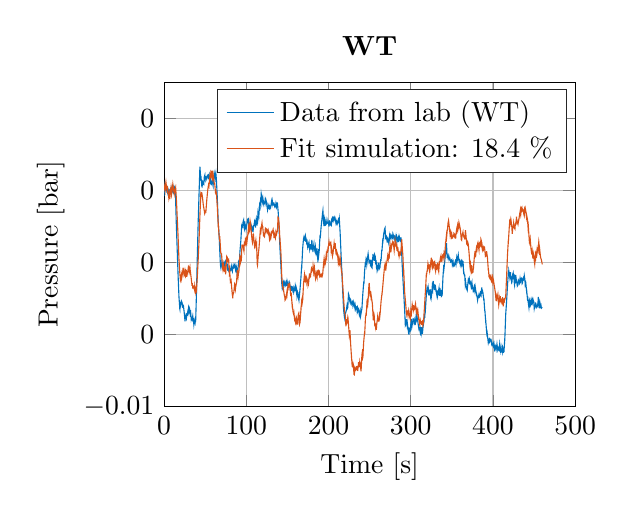
\begin{tikzpicture}

\begin{axis}[%
scaled y ticks = false,
 y tick label style={/pgf/number format/fixed,
/pgf/number format/1000 sep = \thinspace}, % Optional if you want to replace comma as the 1000 separator 
width=2.0556in,
height=1.62135in,
at={(1.011in,0.642in)},
scale only axis,
xmin=0,
xmax=500,
xlabel={Time [s]},
xmajorgrids,
ymin=-0.006,
ymax=0.003,
ylabel={Pressure [bar]},
ymajorgrids,
axis background/.style={fill=white},
title style={font=\bfseries},
title={WT},
legend style={legend cell align=left,align=left,draw=white!15!black}
]
\addplot [color=mycolor1,solid]
  table[row sep=crcr]{%
0.05	-6.8594379276532e-05\\
0.15	-7.81642717496145e-05\\
1.1	0.000151513147605073\\
1.15	0.00014368323558156\\
1.9	6.19041544475118e-05\\
2.75	9.9313734115189e-05\\
3.15	1.66646627564326e-05\\
3.55	5.66842130985679e-05\\
4.3	-7.03343597263789e-05\\
4.65	-9.73040566960709e-05\\
5.25	-3.3794770283424e-05\\
5.35	-7.29443304008093e-05\\
6.25	1.49246823070714e-05\\
6.6	1.4054692082266e-05\\
7.05	-5.46745356791445e-05\\
7.65	-5.03245845551725e-05\\
8.05	2.27545943304319e-05\\
9.1	-6.33744379272272e-05\\
9.35	1.34848485072725e-07\\
9.6	-1.03050342126765e-05\\
9.8	6.53841153474971e-05\\
11.25	-4.77146138802148e-05\\
11.75	7.23440371461215e-05\\
12.25	2.27545943307511e-05\\
12.95	8.01739491698428e-05\\
13.85	-0.000102523998044265\\
14.9	-0.000951634457477868\\
15.95	-0.00163457678396799\\
17.05	-0.00235666867057575\\
18.1	-0.00295000200390924\\
19.15	-0.00329190816226725\\
19.25	-0.00330321803519007\\
19.8	-0.00309964032257974\\
20.2	-0.0031753294721401\\
21.05	-0.00307180063538579\\
22	-0.00311965009775174\\
22.3	-0.00323883875855341\\
23.15	-0.00325101862170134\\
23.4	-0.00319794921798688\\
23.5	-0.00319620923753729\\
24.45	-0.00337977717497578\\
25.5	-0.00363381432062597\\
25.8	-0.00347025615835805\\
27.15	-0.00355812517106641\\
27.5	-0.00343371656891597\\
28.35	-0.00345459633431193\\
28.7	-0.00338934706744946\\
28.85	-0.00340152693059703\\
29.6	-0.00328494824047004\\
30.1	-0.00336237737047919\\
30.4	-0.00324231871945269\\
30.9	-0.00327363836754688\\
31.75	-0.00339804696969642\\
32.15	-0.00332235782013643\\
32.85	-0.00353115547409366\\
32.95	-0.0035137556695967\\
34	-0.00358683484848334\\
34.85	-0.00348765596285314\\
35.05	-0.00353724540566869\\
36.1	-0.00369819359726146\\
36.2	-0.00372081334310709\\
36.75	-0.00360075469208077\\
37.75	-0.00368514374388985\\
38.25	-0.00359205478983309\\
38.4	-0.00365382409579584\\
39.3	-0.00293869213098705\\
40.35	-0.00191210366568881\\
41.4	-0.000950764467252854\\
42.45	-0.000156463391984177\\
43.55	0.00063696769305939\\
43.6	0.000656977468230416\\
44.6	0.000328121163245085\\
45	0.00034552096774132\\
45.55	0.00020023260019475\\
45.75	0.000233292228738274\\
46.5	0.000145423216030172\\
47	0.000223722336264248\\
47.7	0.000169782942324781\\
48.3	0.000160213049850755\\
48.85	0.000363790762460903\\
49.6	0.000422950097749938\\
49.85	0.000324641202344489\\
50.05	0.000304631427173463\\
50.35	0.000384670527857567\\
51.5	0.000362050782013346\\
51.85	0.000322901221896404\\
52	0.00033943103616807\\
52.7	0.000420340127077812\\
53.25	0.000426430058652311\\
53.9	0.000357700830890664\\
54.8	0.000437739931574421\\
55.2	0.00032899115347107\\
56.05	0.000241992130988078\\
56.4	0.000331601124144612\\
57.2	0.00020980249266736\\
57.65	0.000178482844572447\\
58.35	0.00022720229716218\\
58.8	0.000276791739978077\\
59.4	0.000154993108502782\\
59.65	0.000125413440858979\\
60.3	0.000370750684260845\\
60.5	0.000362920772237568\\
61.05	0.000471669550340378\\
62.05	0.000337691055718931\\
62.6	0.000451659775172364\\
62.95	0.000493419305964984\\
63.65	0.000290711583579586\\
64.7	-0.000189523020527521\\
65.8	-0.00086550542522025\\
66.85	-0.00122829134897422\\
66.9	-0.00121698147605158\\
67.9	-0.00176768528836929\\
68.55	-0.00206957189638436\\
69.15	-0.00215657091886683\\
70	-0.00204260219941516\\
70.3	-0.00198431285435212\\
71.1	-0.00210524149560426\\
71.65	-0.00204260219941588\\
72.55	-0.00211307140762684\\
72.75	-0.00205043211143879\\
73.25	-0.00207827179863257\\
73.5	-0.0020025826490724\\
74.45	-0.00195908313783064\\
75.25	-0.00205304208211252\\
76	-0.0020173724828951\\
76.4	-0.00208262174975864\\
77.05	-0.00216179086021817\\
77.5	-0.00210785146627834\\
78.35	-0.00222617013685571\\
79.15	-0.00218441060606522\\
79.45	-0.00224791989247854\\
79.65	-0.00217136075269379\\
80.55	-0.00223487003910462\\
81	-0.00222878010753014\\
81.7	-0.00210611148582919\\
81.75	-0.00210002155425576\\
82.35	-0.00218876055718879\\
83.05	-0.00224878988270133\\
83.8	-0.00211742135875041\\
83.95	-0.00209828157380414\\
84.35	-0.00216179086021639\\
85.25	-0.00214874100684283\\
85.75	-0.00206087199413579\\
86.1	-0.00204608216031203\\
86.95	-0.00220355039100652\\
87.35	-0.00215657091886683\\
87.8	-0.00220442038123252\\
88.05	-0.00215918088954303\\
88.75	-0.0022975093352916\\
89.1	-0.00223574002932848\\
90.15	-0.00211481138807917\\
90.45	-0.00200867258064974\\
91.35	-0.00207740180841226\\
92.3	-0.00169025615836105\\
93.35	-0.00140315938416762\\
94.3	-0.00102906358749066\\
94.5	-0.00105603328445915\\
95.45	-0.000969034261976337\\
95.65	-0.000979474144674752\\
96.15	-0.000861155474098457\\
96.75	-0.000821135923757474\\
97.55	-0.00105864325513677\\
97.7	-0.00107082311828434\\
98.2	-0.000862025464324095\\
98.8	-0.0010812630009817\\
99.4	-0.000946414516133198\\
99.85	-0.00106386319648634\\
100.75	-0.000935104643212684\\
101.5	-0.000805476099712321\\
102.05	-0.000794166226790044\\
102.75	-0.000904654985340925\\
103	-0.000856805522974888\\
103.95	-0.000982954105575182\\
104.4	-0.00108213299120485\\
104.9	-0.000891605131966663\\
105	-0.000932494672533646\\
106	-0.00106038323558166\\
106.2	-0.000992523998044767\\
107.05	-0.00108126300097566\\
107.7	-0.00103776348973354\\
108	-0.00114129232648856\\
108.3	-0.0011447722873872\\
108.7	-0.000982084115343146\\
109.25	-0.000982954105569492\\
110.25	-0.000842015689146144\\
110.3	-0.000844625659820575\\
111.15	-0.00103254354838504\\
111.35	-0.000916834848482456\\
112.15	-0.00078894628543337\\
113.15	-0.00097860415444663\\
113.4	-0.000848975610947336\\
113.55	-0.000929884701856371\\
114.2	-0.000617558211142885\\
115.2	-0.000740226832844179\\
115.6	-0.000560138856304765\\
115.7	-0.000569708748777903\\
116.15	-0.000417460459431196\\
116.75	-0.000471399853371746\\
117.6	-0.00019996290322416\\
117.75	-0.000266952150536848\\
118.15	-9.90440371453488e-05\\
118.75	-0.000186043059628521\\
119.15	-0.000342641300097021\\
120.1	-0.00020953279569802\\
120.75	-0.000340901319647161\\
120.9	-0.000311321652003885\\
121.45	-0.000377440909090573\\
122.35	-0.00037135097751928\\
122.75	-0.000295661827958746\\
123	-0.000356561143696213\\
123.85	-0.000258252248289695\\
124.15	-0.000285221945260317\\
125.1	-0.000435730254157884\\
125.35	-0.000410500537637817\\
125.9	-0.000540129081137111\\
126.2	-0.000506199462369905\\
127.1	-0.000427030351908955\\
127.3	-0.000411370527860611\\
127.8	-0.000504459481918282\\
128.5	-0.000520119305968042\\
128.85	-0.000444430156408215\\
129.6	-0.000473139833826214\\
130.45	-0.000343511290329404\\
130.9	-0.000285221945265299\\
131.45	-0.000361781085048973\\
131.7	-0.000300881769311145\\
132.45	-0.000408760557190802\\
132.6	-0.000408760557190802\\
132.8	-0.000350471212126696\\
133.65	-0.000351341202351266\\
134.65	-0.000464439931578353\\
134.75	-0.000468789882702644\\
135.75	-0.000401800635387126\\
136	-0.000365261045947265\\
136.7	-0.00045748000977823\\
136.85	-0.000440080205279678\\
137.55	-0.000348731231676835\\
137.85	-0.000349601221902127\\
138.9	-0.000634088025422544\\
139.95	-0.00111345263930544\\
141.05	-0.0016537165689226\\
142.1	-0.00209480161291081\\
143.15	-0.00258634608993843\\
143.8	-0.0027342444281605\\
144.5	-0.0026890049364664\\
145.2	-0.00255763641251688\\
145.4	-0.00254023660801976\\
146	-0.00261070581623285\\
146.35	-0.00255328646139474\\
147.4	-0.00263245557185071\\
148.45	-0.00251587688172107\\
148.6	-0.00251413690126838\\
149.2	-0.00265507531769031\\
149.65	-0.00252544677419066\\
150.55	-0.00262723563049547\\
151	-0.00259156603127876\\
151.3	-0.00266812517106174\\
152.1	-0.00264724540566631\\
152.65	-0.00257503621700478\\
152.7	-0.0025819961388035\\
153.6	-0.00277165400781781\\
154	-0.00264898538611688\\
154.6	-0.00279079379276338\\
154.9	-0.00272206456500014\\
155.65	-0.00267508509286329\\
156	-0.00268030503421214\\
156.5	-0.00276817404692237\\
157.1	-0.00271162468230954\\
157.7	-0.00282559340176404\\
158.6	-0.00273424442815695\\
158.95	-0.0027820938905205\\
159.2	-0.00277948391984537\\
159.6	-0.00265681529814514\\
160.7	-0.00280297365591521\\
160.9	-0.00271510464320569\\
161.4	-0.00275947414467238\\
161.75	-0.00294130210166059\\
162.5	-0.00285865303029921\\
163.25	-0.002962181867056\\
163.45	-0.0029334721896373\\
164.1	-0.00304135097752051\\
164.4	-0.00297697170088368\\
165.4	-0.00272554452590483\\
166.45	-0.00242800786901155\\
167.3	-0.00210698147604843\\
167.5	-0.00211307140762186\\
168.6	-0.00160151715541913\\
169.55	-0.00135095997067267\\
170.1	-0.00129702057673639\\
170.65	-0.00138662956989434\\
170.85	-0.00138227961876936\\
171.75	-0.00128049076246384\\
171.9	-0.0012665709188657\\
172.25	-0.00138140962854762\\
172.85	-0.00135791989247777\\
173.4	-0.00145100884653046\\
173.9	-0.00141707922775793\\
174.8	-0.00159368724339515\\
174.95	-0.00158411735092129\\
175.65	-0.00148667844574148\\
176.25	-0.00144056896382636\\
177.05	-0.00162065694036399\\
177.65	-0.00150842820136148\\
178.45	-0.00150581823069273\\
178.85	-0.00165893651026507\\
179.75	-0.0013735797165222\\
180.25	-0.00154061783969055\\
180.55	-0.00153974784946455\\
181	-0.00171026593353402\\
181.3	-0.00161891695992693\\
182.2	-0.00149189838710526\\
182.35	-0.0015597576246425\\
183.25	-0.0016641564516189\\
184.1	-0.00156410757575898\\
184.5	-0.00175115547409745\\
184.85	-0.00177638519061857\\
185.55	-0.00171809584555446\\
185.95	-0.00161456700879838\\
186.6	-0.00183989447702727\\
186.8	-0.00188513396871712\\
187.45	-0.00176681529814401\\
187.8	-0.0018546843108514\\
188.7	-0.00167546632453905\\
189.65	-0.00125004110460025\\
189.95	-0.00132834022483379\\
190.85	-0.00104907336266222\\
191.85	-0.000828965835782888\\
191.9	-0.000832445796681888\\
192.7	-0.000639307966770697\\
193.2	-0.000558398875859886\\
194	-0.000860285483871751\\
194.45	-0.000989044037143991\\
195.1	-0.000836795747801197\\
195.2	-0.000810696041057629\\
196.1	-0.000969904252202683\\
196.55	-0.000964684310853114\\
197.1	-0.000846365640276459\\
197.2	-0.000864635434997457\\
197.7	-0.000925534750735993\\
199	-0.000892475122197978\\
199.3	-0.000840275708706595\\
200.4	-0.000966424291304391\\
200.5	-0.00100470386119766\\
201.35	-0.000853325562075888\\
201.55	-0.000856805522977011\\
202.15	-0.000957724389056544\\
203.4	-0.000975994183772561\\
203.55	-0.000907264956010734\\
203.65	-0.000921184799608163\\
204.55	-0.00079155625611349\\
205.25	-0.000835055767354181\\
205.5	-0.000738486852396095\\
206.1	-0.000748926735095232\\
206.75	-0.000815915982407198\\
207.65	-0.000743706793745663\\
208	-0.000767196529816938\\
208.85	-0.000882905229722716\\
209.15	-0.000925534750736701\\
209.8	-0.000879425268820164\\
210	-0.000858545503424027\\
210.6	-0.00093510464321056\\
211.1	-0.000905524975565147\\
212	-0.000816785972631767\\
212.55	-0.000868115395897165\\
213.1	-0.000783726344087354\\
214.15	-0.0011839218475086\\
215.2	-0.00174941549364901\\
216.25	-0.00225835977517164\\
217.35	-0.00284995312805704\\
218.4	-0.00332931774193851\\
219.3	-0.00350766573802701\\
219.45	-0.00347199613880959\\
219.7	-0.0033910870479002\\
220.65	-0.0034171867546459\\
221.55	-0.00333801764418566\\
222.6	-0.00318054941349045\\
223.1	-0.00323622878788014\\
223.65	-0.00313791989247504\\
223.7	-0.00314400982404918\\
224.3	-0.00287083289345104\\
224.8	-0.0029056325024453\\
225.8	-0.00307267062561364\\
226.35	-0.00311443015640449\\
226.7	-0.00302656114369709\\
226.9	-0.00303526104594425\\
227.95	-0.00312834999999978\\
228.15	-0.00308833044965807\\
228.35	-0.00314139985337475\\
229.1	-0.00309964032258392\\
229.75	-0.00321534902248614\\
230.15	-0.00318228939394528\\
230.6	-0.00310573025416018\\
231.2	-0.00316488958944887\\
232.05	-0.00326493846530951\\
232.45	-0.00318576935484927\\
233.25	-0.0032901681818292\\
233.8	-0.00323709877811323\\
234.45	-0.0032283988758661\\
234.85	-0.00335193748779232\\
235.35	-0.00328929819160392\\
235.65	-0.00335976739981489\\
236.65	-0.00330234804497322\\
237.45	-0.00344937639297213\\
237.5	-0.00345720630499613\\
238.45	-0.00335454745846248\\
238.55	-0.00339891695992989\\
238.95	-0.00349548587488441\\
239.6	-0.00341457678397147\\
240.65	-0.00327450835777127\\
241.7	-0.00288301275660002\\
242.75	-0.0025706862658805\\
243.1	-0.00257590620723078\\
243.85	-0.00225226984359536\\
244.6	-0.0020539120723346\\
244.9	-0.00206957189638401\\
245.8	-0.00188252399804482\\
246.1	-0.00189905381231453\\
246.6	-0.00205217209188403\\
247.15	-0.00195473318670351\\
247.95	-0.00178682507331202\\
248.15	-0.00175898538611646\\
249.15	-0.00195560317693234\\
249.3	-0.0019364633919875\\
250.15	-0.00199475273705019\\
250.45	-0.00193037346041336\\
251.05	-0.00211133142717698\\
251.6	-0.00192254354838794\\
252	-0.00212090131965226\\
252.95	-0.00215135097751867\\
253.35	-0.00200171265884889\\
254.2	-0.00176159535679445\\
254.45	-0.001825104643206\\
255.4	-0.00193559340176008\\
255.75	-0.00193994335288222\\
256.05	-0.00178334511241515\\
256.95	-0.00183728450635498\\
257.55	-0.00206348196481129\\
257.85	-0.00193907336266121\\
258.5	-0.00218789056696138\\
258.8	-0.00213482116324826\\
259.15	-0.00223313005865405\\
260.25	-0.00214091109482523\\
260.8	-0.00200780259042871\\
261.5	-0.00218702057674462\\
262.7	-0.0021322111925795\\
262.9	-0.00203477228739969\\
263.15	-0.00203477228740112\\
263.5	-0.00193124345064716\\
263.95	-0.00193472341154545\\
264.7	-0.00167459633432371\\
265	-0.00167546632455041\\
265.95	-0.00139271950148412\\
266.2	-0.00140750933530255\\
267.15	-0.00121002155427419\\
268.2	-0.00107082311830424\\
268.85	-0.00103776348976338\\
269.1	-0.00124221119259543\\
269.25	-0.00122481138809831\\
269.75	-0.00131442038125555\\
270.35	-0.00128745068428315\\
271.35	-0.00143360904204826\\
271.5	-0.00143360904204683\\
272.15	-0.00133878010753789\\
272.45	-0.00136139985338388\\
273.3	-0.00146927864125927\\
273.5	-0.00144230894429113\\
274.3	-0.00125961099707836\\
274.55	-0.00129528059629506\\
274.85	-0.00135269995113105\\
275.65	-0.00131268040078936\\
275.95	-0.00123177130988067\\
276.8	-0.00127092086999425\\
277.35	-0.00134487003910493\\
277.8	-0.00132834022483024\\
278.3	-0.0012030616324506\\
278.8	-0.00123960122188975\\
279.6	-0.00132573025414585\\
280.2	-0.00129093064515444\\
280.85	-0.00139010953078127\\
280.95	-0.00138749956010825\\
281.9	-0.00127440083087832\\
282.1	-0.00133182018571858\\
282.8	-0.00127614081132604\\
283.05	-0.00130833044964589\\
283.25	-0.00142055918864627\\
284.45	-0.00132486026391632\\
285.05	-0.0014370890029238\\
285.15	-0.00140576935482925\\
285.9	-0.00126483093841301\\
286.2	-0.0012883206744857\\
287.15	-0.0014005494134946\\
287.8	-0.00141707922777357\\
288.2	-0.00130572047899703\\
288.35	-0.00133791011731829\\
289.4	-0.00197735293255874\\
290.45	-0.00244105772239435\\
291.5	-0.00285343308895818\\
292.6	-0.00332409780058895\\
293.45	-0.00375996290322689\\
293.8	-0.00374517306941129\\
294.4	-0.00358596485826551\\
294.85	-0.00358857482893853\\
295.6	-0.00374256309872975\\
295.9	-0.0036860137341162\\
296.8	-0.00384957189638555\\
297	-0.00380172243402341\\
297.9	-0.00400530014663303\\
298.4	-0.00385044188661082\\
299.4	-0.00389307140762979\\
300	-0.00372255332356387\\
300.7	-0.00357117502444423\\
301.05	-0.00373125322581386\\
301.3	-0.00379650249267598\\
302.1	-0.00369297365591137\\
302.9	-0.00356508509286158\\
303.6	-0.00357117502443854\\
304	-0.00364686417399837\\
304.35	-0.00359901471163339\\
305.3	-0.00372342331378206\\
305.35	-0.00374169310850304\\
306.35	-0.00352332556206647\\
306.6	-0.00347025615835263\\
307.3	-0.00357900493646468\\
307.7	-0.00352245557185539\\
308.4	-0.00364338421310434\\
308.45	-0.00362424442815806\\
309.5	-0.00378171265886038\\
309.65	-0.00373821314762039\\
310.2	-0.00384696192572391\\
310.6	-0.00383304208212222\\
311.55	-0.00394092087001324\\
311.95	-0.00385566182797815\\
312.7	-0.00396702057674615\\
313.4	-0.00379650249267739\\
314.15	-0.00398355039100948\\
314.85	-0.00381912223851627\\
315.85	-0.00365817404693131\\
315.95	-0.00367818382210287\\
316.75	-0.00343632653959929\\
317	-0.00353550542523037\\
317.9	-0.00323361881721779\\
318	-0.0032492786412672\\
319.05	-0.0028882326979638\\
319.85	-0.00269857482894592\\
321	-0.00281080356794489\\
321.2	-0.00275338421310606\\
321.35	-0.00271684462366266\\
322.25	-0.00288388274682887\\
322.4	-0.00291781236559785\\
322.8	-0.00276904403715263\\
323.65	-0.00276643406647678\\
324.1	-0.00290737248290156\\
324.35	-0.00286648294233173\\
324.9	-0.00297871168133496\\
325.45	-0.00288301275660358\\
326.2	-0.00266290522971928\\
326.75	-0.00274033435972824\\
327.3	-0.00251326691104878\\
328.1	-0.00271771461388083\\
328.5	-0.00259765596285005\\
328.85	-0.00277078401759183\\
329.05	-0.00263332556206819\\
329.9	-0.00263506554252728\\
330.55	-0.00276904403715832\\
330.75	-0.00276295410558702\\
331.35	-0.00286561295212351\\
331.95	-0.0029378221407822\\
332.55	-0.00277861392964068\\
332.85	-0.00289954257089106\\
333.9	-0.00277165400784411\\
334.35	-0.00271423465300386\\
334.8	-0.00292564227763675\\
334.95	-0.00287257287392151\\
335.45	-0.00270727473119307\\
336.5	-0.00292738225806316\\
336.9	-0.00276034413489269\\
337.1	-0.00282559340175338\\
337.35	-0.00294043211143247\\
338.2	-0.00291694237536545\\
339.2	-0.00240364814271429\\
339.95	-0.0021600508797644\\
340.3	-0.00219659046920923\\
341.35	-0.00197909291300646\\
342.35	-0.00164501666667546\\
342.55	-0.00168416622679329\\
343.45	-0.00146753866080444\\
344.35	-0.00187382409579839\\
344.65	-0.001810314809384\\
345.5	-0.00189644384164295\\
345.55	-0.00188948391984353\\
346.25	-0.00181118479960786\\
346.8	-0.00186338421309641\\
347.35	-0.00191819359725513\\
347.7	-0.00190079379275658\\
348.65	-0.00199388274681211\\
349	-0.00198692282500984\\
349.35	-0.0019329834310693\\
350.05	-0.0019181935972466\\
350.6	-0.00206957189636908\\
351.55	-0.00198866280545756\\
351.8	-0.00205478206254354\\
352	-0.00204521217007396\\
352.55	-0.0021061114858196\\
353	-0.00209132165199263\\
354.05	-0.00197735293255163\\
354.2	-0.00196430307918091\\
355.05	-0.00205913201368702\\
355.1	-0.00204869213098929\\
355.95	-0.00186599418378364\\
356.55	-0.00195125322582014\\
357.25	-0.00186164423265722\\
357.8	-0.00179117502445052\\
358.3	-0.0019208035679523\\
358.8	-0.00196430307918943\\
358.95	-0.00191210366570088\\
359.4	-0.00192167355817047\\
360.4	-0.00203999222874357\\
360.45	-0.00206174198436428\\
361.35	-0.00197996290322605\\
361.85	-0.00206609193548643\\
362.45	-0.00199127277614763\\
362.8	-0.00203042233626405\\
363.05	-0.00196865303030022\\
363.65	-0.00197474296187436\\
364.4	-0.00232534902247862\\
364.65	-0.00227923954056421\\
365.35	-0.0023636285923726\\
365.7	-0.00236014863147431\\
366.3	-0.00261244579667134\\
366.8	-0.00254110659823083\\
367.8	-0.00272206456500299\\
368.7	-0.00277600395894211\\
368.9	-0.00271423465298254\\
369.95	-0.00248977717497609\\
370.65	-0.0025350166666709\\
371	-0.00244453768328412\\
371.1	-0.00243670777126226\\
372.05	-0.00258025615836571\\
372.9	-0.00254719652981492\\
373.1	-0.00263506554252159\\
373.5	-0.00268030503421214\\
374.2	-0.00259678597263188\\
374.45	-0.00256807629521602\\
374.75	-0.00269248489736611\\
375.3	-0.00266986515151728\\
376.1	-0.00281080356794063\\
376.55	-0.00279601373412219\\
377.35	-0.00268900493646923\\
377.9	-0.00277687394917449\\
378.4	-0.00267769506354625\\
379.45	-0.00284212321603944\\
379.55	-0.00282559340176902\\
380.55	-0.0029195523460484\\
381.3	-0.0030457009286448\\
381.65	-0.00298480161290768\\
382.65	-0.00292390229716771\\
382.9	-0.00289693260019816\\
383.35	-0.00296914178885685\\
383.95	-0.00295174198436114\\
384.8	-0.00284734315737409\\
385.55	-0.00290476251222287\\
385.85	-0.00281254354839404\\
386.45	-0.00269770483871495\\
386.9	-0.00282472341153947\\
387.4	-0.00280471363637359\\
387.95	-0.00287866280548996\\
388	-0.00287692282503939\\
388.8	-0.00303004110460675\\
389.05	-0.0030248211632579\\
390	-0.00334149760509461\\
390.1	-0.0033075679863242\\
391.15	-0.00363033435973505\\
391.25	-0.00362685439883534\\
392.2	-0.0039009013196545\\
392.25	-0.00389742135875479\\
393	-0.00407141940371331\\
393.25	-0.00401487003909834\\
394.3	-0.00423323758553208\\
395.35	-0.00412970874877884\\
395.75	-0.00411839887585443\\
396.05	-0.00420800786901451\\
396.9	-0.00417146827958105\\
397.15	-0.00413057873900981\\
397.55	-0.00413231871946038\\
398.4	-0.00425672732161046\\
398.7	-0.00422540767351876\\
399.55	-0.00429065694038228\\
400.35	-0.00432806652005381\\
400.65	-0.00424541744869031\\
401.05	-0.00421931774194034\\
401.65	-0.00434459633431145\\
401.75	-0.00432893651026346\\
402.25	-0.00440462565982329\\
403	-0.00433241647115891\\
403.85	-0.00442376544476814\\
404.85	-0.00426803719452493\\
404.9	-0.00427847707722122\\
405.9	-0.00444029525903857\\
406.05	-0.00442985537634086\\
406.4	-0.00436634608992505\\
407.55	-0.00442811539589029\\
408.1	-0.00429152693059477\\
408.2	-0.00426455723362379\\
409.05	-0.00442028548386558\\
409.15	-0.00439244579666932\\
409.8	-0.00449336466274103\\
410.4	-0.00448640474094446\\
410.95	-0.00435329623654865\\
411.7	-0.00447248489735272\\
412.05	-0.00438635586510372\\
412.35	-0.00441854550342213\\
413.1	-0.00448553475073196\\
413.4	-0.00447596485826379\\
414.4	-0.00411056896383399\\
414.45	-0.00411317893450841\\
415.5	-0.00344241647116632\\
416.55	-0.00309616036168563\\
417.65	-0.00265768528836757\\
418.7	-0.00229402937438833\\
419	-0.00231403914956131\\
419.25	-0.00223226006843019\\
419.75	-0.0023009892961906\\
420.5	-0.00242278792767478\\
421.35	-0.00226966964810457\\
421.7	-0.00242452790812535\\
422	-0.0024140880254248\\
422.85	-0.00256807629522028\\
423	-0.00256198636364614\\
424	-0.00232708900294482\\
424.6	-0.00228619946238637\\
425.05	-0.00241321803520946\\
425.45	-0.00239320826003364\\
426.1	-0.00261157580646737\\
426.25	-0.00262984560118411\\
426.65	-0.0024271378787955\\
427.3	-0.00248977717498178\\
427.65	-0.00234970874878512\\
428.25	-0.00245758753666052\\
429.25	-0.00260026593352874\\
429.35	-0.00259243602150405\\
429.65	-0.00265681529813661\\
430.5	-0.00262462565982104\\
431	-0.00249151715541529\\
431.5	-0.00251239692081781\\
432.2	-0.00256981627565664\\
432.8	-0.00247237737047327\\
433.15	-0.00257764618768135\\
433.55	-0.00250369701856924\\
434.5	-0.00243409780057788\\
434.65	-0.00243409780058072\\
435.45	-0.00258895606060718\\
435.9	-0.00257068626588761\\
436.3	-0.00246019750732784\\
437.3	-0.00240973807428985\\
437.45	-0.00248803719452267\\
437.75	-0.00248281725317809\\
438.15	-0.00237232849462543\\
438.85	-0.00247063739003407\\
439.25	-0.00263071559140654\\
439.95	-0.002581126148591\\
440.95	-0.00281080356794347\\
441.1	-0.00280210366569775\\
442	-0.00301873123168234\\
442.45	-0.00299785146628977\\
443.05	-0.00313443993158244\\
443.75	-0.00325275860215839\\
444.25	-0.00311617013685861\\
445	-0.0032501486314797\\
445.4	-0.00310312028348504\\
445.8	-0.00316314960900115\\
447	-0.00304483093842661\\
447.3	-0.00313182996090944\\
447.55	-0.00318837932552582\\
448.3	-0.00301177130988577\\
448.45	-0.00300133142718663\\
449.35	-0.00309355039101972\\
449.5	-0.00306658069405016\\
450.2	-0.00328407825025294\\
450.5	-0.00325014863148254\\
451.55	-0.00316053963832245\\
451.7	-0.00311008020528163\\
452.25	-0.00321099907136044\\
452.6	-0.00318489936461616\\
453.3	-0.00324927864125441\\
454	-0.00322317893451297\\
454.75	-0.00311443015640661\\
455.2	-0.00295609193548897\\
455.8	-0.00315879965787615\\
456	-0.00313878988270316\\
456.65	-0.00327450835777766\\
457.2	-0.0031257400293353\\
457.9	-0.00321621901271782\\
458.4	-0.00318663934507241\\
458.95	-0.00326754843598109\\
460	-0.00324144872924392\\
};
\addlegendentry{Data from lab (WT)};

\addplot [color=mycolor2,solid]
  table[row sep=crcr]{%
0.05	0\\
0.25	0.000126139876466886\\
1.25	-1.05983673427483e-05\\
2.2	0.000227359321848562\\
2.25	0.000234806646036057\\
3.2	4.17680913403206e-05\\
3.55	8.37125820886855e-06\\
4	0.000124926781289701\\
4.3	6.10460752435084e-05\\
5.35	-0.000125272414446176\\
5.8	-0.000213556797919882\\
6.45	-0.000109472736706682\\
7	-0.000244256525070616\\
7.5	-1.86146423551351e-05\\
7.85	-4.28913925451429e-05\\
8.5	8.79722805623285e-05\\
8.55	7.93261715833282e-05\\
9.1	-0.00011530667522843\\
9.6	-4.93073971266936e-05\\
10.65	0.000171314414775133\\
11.55	1.47842649782147e-05\\
11.8	3.35040429245553e-05\\
12.45	-0.000100325825542133\\
12.8	-5.21775457591674e-05\\
13.85	5.38120006752561e-05\\
14.1	7.68869027947767e-05\\
14.9	-0.000206498456320705\\
15.95	-0.000728654407974497\\
17.05	-0.00128482371678666\\
18.1	-0.00191476341862683\\
19.15	-0.00229827295255912\\
19.9	-0.00249932716195906\\
20.6	-0.0024431970825516\\
21.1	-0.00235689719101507\\
21.4	-0.0024416634195548\\
22.35	-0.00231255683415496\\
23.2	-0.00214331866150934\\
23.4	-0.00220940797760628\\
24.2	-0.0023387055800451\\
25.1	-0.00223917083516032\\
25.4	-0.0023623965168082\\
26	-0.00239083560121942\\
26.4	-0.00220667814578566\\
27	-0.00222106595704536\\
27.6	-0.00239790818765249\\
27.65	-0.00238417339276948\\
28.7	-0.00226890518943875\\
29.65	-0.00211072569753362\\
30	-0.00212391513149743\\
30.6	-0.00226105004315843\\
30.8	-0.00223451844361599\\
31.5	-0.00213752698426758\\
31.85	-0.00223254811159493\\
32.95	-0.00242710217694942\\
34	-0.00264847805846848\\
34.2	-0.00257831225091556\\
35.05	-0.0027208865359478\\
35.1	-0.00272132536156876\\
35.7	-0.00268411899549652\\
36.3	-0.00266212061444774\\
37	-0.0027487396782647\\
37.3	-0.00265469458992753\\
38.2	-0.00280767961484576\\
38.5	-0.00273951834409263\\
39.25	-0.0028097816158882\\
39.3	-0.00280541545593148\\
40.35	-0.00242706070453612\\
41.4	-0.00196618152625428\\
42.45	-0.00143980990369244\\
43.55	-0.000734322890876339\\
44.55	-0.000161223685619334\\
44.65	-0.000174951432214615\\
45.2	-6.0954717272807e-05\\
45.95	-6.85274667973505e-05\\
46.65	-0.000208387583599108\\
46.75	-0.000202502536995651\\
47.75	-0.000413004919720121\\
48.85	-0.000554033653279941\\
49.45	-0.000647699998003968\\
50.05	-0.000612562867429424\\
50.8	-0.000551676462294452\\
50.95	-0.00056071975702923\\
52	-0.000252225825046416\\
53.05	1.92774391184723e-07\\
54.05	0.0001532866604495\\
54.6	0.000114509631259366\\
55.2	0.000259763291619735\\
55.95	0.000428022960124995\\
56.45	0.000399677189355968\\
57.05	0.00053393921850067\\
57.4	0.000523410045502986\\
58.05	0.000351164688281058\\
58.6	0.000309313267065626\\
59.25	0.000548902685755198\\
59.4	0.000490080322920536\\
60.45	0.000300362418108328\\
60.55	0.000304042781740661\\
61	0.00019858502362409\\
61.55	0.000198879084350754\\
62.6	-7.14067570665315e-05\\
62.9	-8.80185179459432e-05\\
63.35	-4.50448961835394e-05\\
63.65	-7.78567256744941e-05\\
64.7	-0.000433494784207036\\
65.75	-0.000911246326598635\\
65.85	-0.000900715045675105\\
66.85	-0.00124183863866182\\
67.5	-0.00136159643656144\\
67.9	-0.00133889324592364\\
68.95	-0.00173370341239143\\
69.95	-0.00179752033356916\\
70	-0.00179565686749285\\
71.1	-0.00214445537543593\\
71.5	-0.00219851183057646\\
71.85	-0.00212838178774389\\
72.35	-0.00205977634496857\\
73	-0.00225430152623098\\
73.3	-0.00211773701215098\\
73.65	-0.00219023196156648\\
74.25	-0.00213979211684557\\
74.85	-0.00232929369058777\\
75.3	-0.0021847962114048\\
76.25	-0.00183464077316149\\
76.9	-0.00186611463810704\\
77.3	-0.00198641640068297\\
78.25	-0.00198805412211145\\
78.5	-0.00189144602965671\\
79.3	-0.00226991029734343\\
79.75	-0.00221497246889408\\
80.6	-0.00251823024136217\\
80.65	-0.00251517694276553\\
81.55	-0.00257057794022287\\
81.7	-0.00254932750817681\\
82.65	-0.00280811221994695\\
82.75	-0.00280103156895386\\
83.6	-0.00299625784327503\\
83.8	-0.00289976312267446\\
84.85	-0.00282225032665403\\
85.85	-0.00259785463998668\\
85.9	-0.00260063809480404\\
86.75	-0.00274398154552447\\
87	-0.00269314896356743\\
88.05	-0.00257025066699326\\
89.1	-0.00221789448455133\\
90	-0.00240256630874888\\
90.15	-0.00237557885248966\\
91.1	-0.00218300778820366\\
91.2	-0.00219171497865203\\
92.05	-0.00188272893017179\\
92.8	-0.00199136292094166\\
93.35	-0.00186455908374568\\
94.05	-0.00191032278696757\\
94.4	-0.0016678780156479\\
94.85	-0.00151716041946478\\
96.05	-0.00152440411020537\\
96.5	-0.0016144627987152\\
97.15	-0.00168256367067791\\
97.6	-0.00146628956103933\\
98.2	-0.00149486649943233\\
98.65	-0.00143011388365201\\
99.05	-0.00131222400933689\\
99.65	-0.00148150494457127\\
99.7	-0.001477859870524\\
100.1	-0.0012765934532745\\
100.75	-0.0014340255531874\\
101.8	-0.00123904963845932\\
102.85	-0.000993680556370352\\
102.9	-0.000987852422910172\\
103.45	-0.00115309823304283\\
104.05	-0.0011147702588537\\
104.7	-0.000857173040904633\\
105.5	-0.000960806795994099\\
106.05	-0.00116199962855866\\
107.1	-0.00139654048647017\\
107.5	-0.00144724670239795\\
108.15	-0.00131112339771395\\
108.6	-0.00119715128062759\\
109.25	-0.00137080784687398\\
110.25	-0.00158281633618395\\
110.3	-0.00158038243775916\\
111.35	-0.00141014615722672\\
111.6	-0.00137960690306836\\
112.2	-0.00155118439427895\\
112.55	-0.00151990174409864\\
113.3	-0.00204823676604827\\
113.6	-0.00207860566125334\\
114.55	-0.00179851202103195\\
115.6	-0.00155911685199906\\
116.65	-0.00122475103070055\\
117.1	-0.00109316553824441\\
117.75	-0.00114967434291994\\
118.65	-0.000966303705408927\\
119.1	-0.000905815564803955\\
119.75	-0.00105688869181547\\
119.95	-0.000996450653764822\\
120.9	-0.00124367609077152\\
121.45	-0.00122577608473779\\
121.9	-0.00128437137134542\\
122.1	-0.00129039614288627\\
123	-0.00112119580030307\\
123.25	-0.00102661834590948\\
123.95	-0.0011903243346693\\
124.05	-0.00116136429024273\\
124.75	-0.0010740246944342\\
125.4	-0.00108159357216057\\
126.05	-0.00118342505284983\\
126.45	-0.00120322095216793\\
126.9	-0.00112522302344699\\
127.3	-0.00116966903858715\\
128.25	-0.0013586770467813\\
128.3	-0.00135350671210857\\
128.95	-0.00122269933823595\\
129.8	-0.00132631258850373\\
130.45	-0.00124537139781068\\
130.95	-0.00115261370754178\\
131.5	-0.0011705592758119\\
132.55	-0.001089907876669\\
132.6	-0.0010861621367266\\
133.6	-0.00126879837587358\\
133.75	-0.00132273736775101\\
134.25	-0.00120850131502571\\
134.65	-0.00123866735159479\\
135.4	-0.00131918590420578\\
135.75	-0.00125079076170678\\
136.05	-0.00115061310640337\\
136.8	-0.00121467577521731\\
137.75	-0.00113391004362675\\
137.85	-0.00115428920626748\\
138.6	-0.000747250475366935\\
139.1	-0.00076765199816725\\
139.95	-0.000948131083989251\\
141.05	-0.00143522805170494\\
141.2	-0.00142351137001554\\
142.1	-0.0017259315406505\\
143.15	-0.00239017956498325\\
144.2	-0.00266999594420311\\
145.25	-0.00277843922096699\\
145.35	-0.00276648086235649\\
146.25	-0.00291387108831712\\
146.6	-0.00290928769069577\\
147.15	-0.00305089422315992\\
147.85	-0.00302641815280997\\
148.15	-0.00296054593810244\\
148.45	-0.00296187649626556\\
149.25	-0.00283592040686931\\
149.55	-0.002894234987516\\
150.55	-0.00266874052407379\\
150.95	-0.00270886402448392\\
151.4	-0.00262327059238572\\
151.95	-0.00264663484249132\\
152.4	-0.00260955605193433\\
152.8	-0.00259297669694845\\
153.6	-0.00281338513792498\\
153.75	-0.00279165887682085\\
154.8	-0.00293608894364604\\
154.9	-0.00292891894152958\\
155.75	-0.00318580718730899\\
155.9	-0.00317138463565717\\
156.9	-0.00337945229501686\\
157.95	-0.0034665908870115\\
158.1	-0.00343308900071586\\
158.8	-0.00359255043058185\\
159.05	-0.00358119314988779\\
159.9	-0.00366732546187953\\
160.45	-0.0035695069809847\\
160.85	-0.00364142318074094\\
161.25	-0.00358641024467846\\
161.8	-0.00370076841812269\\
162.55	-0.00371035927956934\\
163.3	-0.0034363131479529\\
163.85	-0.0034053100052954\\
164.35	-0.00353985559378171\\
164.85	-0.00370928411648955\\
165.4	-0.0036602031911176\\
166.45	-0.00330901255640915\\
166.5	-0.00331413554392929\\
167.5	-0.00303110306883028\\
167.8	-0.00300305077577843\\
168.15	-0.00310415193170468\\
168.6	-0.00303684673802055\\
169.65	-0.00258130638398772\\
170.7	-0.00235370718665873\\
170.75	-0.00234468007455592\\
171.6	-0.00254991384486262\\
171.85	-0.00244184818245378\\
172.8	-0.0025476447224248\\
173.1	-0.00240956197028297\\
173.9	-0.00245773576843946\\
174.95	-0.00259917732969905\\
175	-0.00261297092281221\\
175.85	-0.0024858154789119\\
176	-0.00251689663432983\\
176.95	-0.00230558131133264\\
177.05	-0.00233422460961665\\
177.45	-0.00241448983281962\\
178.1	-0.00239096576330944\\
179.2	-0.00216334559818165\\
179.25	-0.00216034804206886\\
179.8	-0.00224860546851634\\
180.85	-0.00220455797676151\\
181.25	-0.0020888049839394\\
181.3	-0.00209747483295958\\
182	-0.00227838009002048\\
182.85	-0.00214810133061132\\
183.3	-0.00228461811984169\\
183.4	-0.00227340400267483\\
184.25	-0.00244711499133983\\
184.7	-0.00238810863177321\\
185.05	-0.00231057487295813\\
186.1	-0.00242651857578182\\
186.55	-0.00226566790860955\\
187.25	-0.00230317479382347\\
187.65	-0.002248731924535\\
187.95	-0.00219878341428102\\
188.2	-0.00235945609404461\\
188.8	-0.00221908486942009\\
189.45	-0.00240794111111443\\
190.45	-0.00238802762179769\\
190.8	-0.00232807877206575\\
191.1	-0.00232328012640183\\
191.8	-0.00240545726686402\\
192.1	-0.00240451290408591\\
192.95	-0.0023118830001635\\
194	-0.00203165320968471\\
194.65	-0.00189457768601759\\
195.55	-0.0020601436621105\\
196.15	-0.00198029162667662\\
196.25	-0.00198803705571994\\
197.15	-0.00179366770571675\\
197.75	-0.00185981947352011\\
198.25	-0.00168197555479116\\
198.85	-0.0016989819828385\\
199.3	-0.00161198427390824\\
199.6	-0.00162881829908551\\
200.4	-0.00146042514585518\\
200.6	-0.00142629608002283\\
201.15	-0.0015231414574333\\
201.8	-0.00151810317696417\\
202.5	-0.0014518226613543\\
202.7	-0.00144403978109938\\
203.25	-0.00167723052703589\\
203.75	-0.00160478435505079\\
204.5	-0.00172094752272544\\
204.85	-0.00180805030350469\\
205.55	-0.00170016533588824\\
205.65	-0.00170941538823076\\
206.75	-0.00148540867124375\\
206.8	-0.00147470563741615\\
207.45	-0.00162118318819779\\
208.1	-0.00146672053727775\\
208.75	-0.00166030443910449\\
208.85	-0.0016448920972855\\
209.75	-0.00174296383229312\\
210.05	-0.00169548507361015\\
210.95	-0.00177556641990034\\
211.85	-0.00200248179901924\\
212.45	-0.00190283691228758\\
213.1	-0.00204962396080092\\
213.15	-0.00205278554796682\\
214.15	-0.00187708548908877\\
215.2	-0.00212645408294641\\
215.9	-0.00226330889814092\\
216.25	-0.0022584877254861\\
217.35	-0.00265968223577206\\
218.4	-0.00301865639987681\\
219.45	-0.00337055380992505\\
220.5	-0.00347807090160976\\
221.15	-0.00377325787778322\\
221.75	-0.00357845356924677\\
222.35	-0.00368742105894339\\
222.65	-0.0036761510756003\\
223.5	-0.00351990880756637\\
223.7	-0.00354141521876423\\
224.75	-0.00386051279426583\\
225.25	-0.00401813331901321\\
226.05	-0.00388390890826022\\
226.85	-0.00424146050152242\\
227.9	-0.00461004865757388\\
227.95	-0.00460614306756105\\
228.8	-0.00488212913103924\\
229.6	-0.00490194766870463\\
229.95	-0.00481353389872753\\
230.05	-0.00482224368683454\\
231.05	-0.00511124486126625\\
231.4	-0.00511866444172109\\
232.1	-0.00491944314448502\\
232.15	-0.00492248725030835\\
232.95	-0.0049811717396419\\
233.3	-0.00496518023015645\\
234.15	-0.00489113710406438\\
234.5	-0.00489214702859116\\
235.05	-0.00499532693368121\\
235.5	-0.00499810059499524\\
236.4	-0.00481728638374816\\
236.55	-0.00477070684335446\\
237.25	-0.00489588051249119\\
237.55	-0.00489332238378593\\
238	-0.00475712127387675\\
238.55	-0.00482298173368067\\
239.55	-0.00502493700526405\\
239.6	-0.00501153890419076\\
240.65	-0.00455982647797128\\
240.9	-0.00452095188435292\\
241.55	-0.00465233462398519\\
241.8	-0.00463103250104227\\
242.75	-0.00421079876689849\\
243.85	-0.00394406747496671\\
244.1	-0.00395125267185139\\
244.9	-0.00354803128172979\\
245.6	-0.0034261302252693\\
245.95	-0.00343666452445922\\
246.95	-0.00303976300522365\\
247.25	-0.00303010218445802\\
247.8	-0.00314577994463434\\
248.05	-0.00308719640674559\\
249.15	-0.00262174553690272\\
249.45	-0.00256746422679186\\
250.2	-0.00281643860640263\\
250.6	-0.00294790778990606\\
251.25	-0.00280123274508161\\
251.95	-0.00305026133345014\\
252.3	-0.00298311588867994\\
253.35	-0.00314741595115309\\
254.45	-0.00360447326358141\\
255.35	-0.00343862049197151\\
255.5	-0.00345406761823956\\
256.35	-0.00377131085134697\\
256.65	-0.00368281260819677\\
257.2	-0.00379515403455647\\
257.75	-0.00370357724039053\\
258.15	-0.00387079370245318\\
258.65	-0.00370619068405218\\
259.7	-0.00353514961406362\\
259.75	-0.00352019887895398\\
260.35	-0.00362518643920873\\
260.85	-0.00362815826589454\\
261.85	-0.00347171058216165\\
262.25	-0.00352722810907717\\
262.9	-0.00338055412026302\\
263.95	-0.00307235311844509\\
265	-0.00287175081328894\\
265.1	-0.00287307850490891\\
266.1	-0.002633700853552\\
267.15	-0.00235342692161954\\
268.2	-0.00210934407234056\\
268.8	-0.00204612761650191\\
269.25	-0.00215073849127421\\
269.6	-0.00222981883644045\\
270.3	-0.00206821138326424\\
271.4	-0.00191521748561448\\
272	-0.00181463908420801\\
272.7	-0.00191225768792993\\
273.3	-0.00181027418225772\\
273.7	-0.00190334278091227\\
274.55	-0.00157165022775434\\
274.9	-0.00149472844969039\\
275.6	-0.0016382907374157\\
275.8	-0.00171698401083955\\
276.6	-0.00155813833568946\\
276.7	-0.00156832428346633\\
277.75	-0.00143908847756614\\
278.45	-0.00148810403254964\\
278.7	-0.00141765395090244\\
278.8	-0.00144485168254453\\
279.85	-0.00166809916489637\\
280.9	-0.0014195319239922\\
281	-0.0013837554340994\\
282	-0.00153395625878766\\
282.55	-0.00151902885889178\\
282.8	-0.00156587720008814\\
283.1	-0.0015215879951336\\
284	-0.00168872357247333\\
284.25	-0.00157553901880612\\
285.15	-0.00177202382691008\\
285.65	-0.00174746312621668\\
285.95	-0.00182284449981682\\
286.45	-0.00175541584942702\\
286.9	-0.00180070713922967\\
287.4	-0.00179357513189909\\
288.15	-0.00165089451040519\\
288.35	-0.00165836401438322\\
289.05	-0.00136269753736502\\
289.4	-0.0014918763272872\\
290.45	-0.0018074052954544\\
291.45	-0.00230766804951929\\
291.6	-0.00229139500775606\\
292.6	-0.00282763204056935\\
293.65	-0.00309802319843803\\
294.7	-0.00339257172835011\\
295.1	-0.00344805593925678\\
295.75	-0.00335559138280214\\
296.4	-0.0033426025751642\\
296.8	-0.00345982363285998\\
297.55	-0.00332679171199649\\
297.9	-0.00336939907270387\\
298.95	-0.00354259478450308\\
299.4	-0.00357681512973253\\
300	-0.00337859311167304\\
300.15	-0.00333581056941573\\
300.85	-0.00341326928047897\\
301.05	-0.00334169905649757\\
301.8	-0.00316627138188151\\
302.1	-0.003207031743046\\
303.1	-0.00331748123616644\\
303.45	-0.00318569124139751\\
303.9	-0.00332353505498789\\
304.85	-0.00328933227487005\\
305.3	-0.0032012328180699\\
305.8	-0.00314727336108428\\
306.35	-0.00328890720407897\\
306.95	-0.00339345228976585\\
307.6	-0.00331730384498684\\
308.4	-0.00342175867184548\\
308.75	-0.00336352435302679\\
309.55	-0.00354257573128954\\
309.75	-0.00353416443830261\\
310.6	-0.00370178950697577\\
311.55	-0.00360372099787824\\
311.65	-0.00361850532136981\\
312.7	-0.00370905517451392\\
312.8	-0.00373435190777306\\
313.1	-0.00365801426436144\\
314.1	-0.00362841564389452\\
314.75	-0.00375196582043366\\
315.05	-0.00372569432233158\\
315.9	-0.00353689537156284\\
316.95	-0.00313740355356253\\
318	-0.00274796886046957\\
319.05	-0.00229242373956225\\
319.25	-0.00234150911036039\\
319.95	-0.00222589315786228\\
320.15	-0.00222748478981376\\
320.95	-0.00202881361218999\\
321.2	-0.00205522495616022\\
322.25	-0.00217602128302743\\
322.7	-0.00205840461679717\\
323.25	-0.00222407586573844\\
323.3	-0.00221691323025846\\
324.35	-0.00199534481382146\\
325.1	-0.00187110597407204\\
325.45	-0.00203575965719309\\
325.8	-0.00209264824533308\\
326.4	-0.00201405210673287\\
326.85	-0.00212854726226763\\
327.55	-0.00204776919566559\\
327.7	-0.00206416554642851\\
327.95	-0.00199458559493125\\
329.1	-0.00197111423912251\\
329.35	-0.00215043060820358\\
330.2	-0.0022448933248379\\
330.75	-0.00210867398668045\\
331.25	-0.00214172932522077\\
331.5	-0.00207550805542876\\
332.25	-0.00204867203419596\\
332.65	-0.00212428847994022\\
333.05	-0.00207908876975553\\
333.8	-0.00223142110254994\\
334.05	-0.0022568514869085\\
334.95	-0.0019749617391628\\
335.65	-0.00198044770685641\\
336.05	-0.00187227838468817\\
336.7	-0.00181796310175533\\
337.1	-0.00192848572508115\\
337.65	-0.00190819475203005\\
337.8	-0.00198303774514376\\
338.15	-0.00190936662629924\\
338.75	-0.00179934248821261\\
339.8	-0.00176891252518059\\
340.25	-0.00188655680650945\\
340.3	-0.00189293019237704\\
340.65	-0.00174151507907969\\
341.55	-0.00181565400525265\\
342.25	-0.00146749776872552\\
342.4	-0.00146901965680356\\
343.45	-0.00124248919397059\\
343.7	-0.00128582170729156\\
344.5	-0.00108196488697258\\
344.6	-0.00111052427485811\\
345.35	-0.000908177761890697\\
346	-0.000838171205375932\\
346.65	-0.000969254573643338\\
347.65	-0.00117789279991772\\
348	-0.00125488724772084\\
348.7	-0.00116026401392958\\
349.3	-0.00124458115042124\\
349.65	-0.0011495501282667\\
349.8	-0.00120151682941177\\
350.35	-0.001328530987848\\
350.9	-0.0013199091041389\\
351.8	-0.00124953073954462\\
352.2	-0.00125934186347464\\
352.5	-0.00119295493501697\\
353.15	-0.00121484556547517\\
353.65	-0.00131723366519614\\
354.65	-0.00132483978753396\\
355.1	-0.00119153479839992\\
355.9	-0.0010759688201991\\
356.15	-0.00111223846032112\\
356.95	-0.000979994126290765\\
357.4	-0.00107376116876768\\
357.9	-0.000985185278050442\\
358.3	-0.00101261654280272\\
358.65	-0.000891792298343839\\
359.45	-0.000970146108812116\\
360.4	-0.00108983012549336\\
361.45	-0.00136597489243325\\
361.9	-0.00138192917360391\\
362.5	-0.00125270660737783\\
363.5	-0.00116159283943965\\
363.6	-0.00118735176918273\\
364.65	-0.00129350946291355\\
365.4	-0.00127216939923442\\
365.7	-0.0013414888287632\\
365.8	-0.00136664422539489\\
366.5	-0.0011037387756892\\
366.75	-0.00115132579273934\\
367.8	-0.00140345129243405\\
367.9	-0.00139297813628052\\
368.85	-0.00151825923242846\\
369.2	-0.00152724039888378\\
369.55	-0.00145678563769786\\
370	-0.00149947685505211\\
371	-0.00175140306538598\\
372.05	-0.00212194374189731\\
372.2	-0.00214931503706156\\
372.75	-0.00206164968882069\\
373.35	-0.00221698590349832\\
374.05	-0.00207850135352821\\
374.2	-0.00211921105994134\\
374.55	-0.00229196118459773\\
375.7	-0.00226915311050094\\
376.3	-0.00211851527074474\\
376.4	-0.00212553755067192\\
377.35	-0.00185467445390463\\
378.3	-0.00167942967398649\\
378.85	-0.0018584681866336\\
379.5	-0.00166540483132143\\
379.8	-0.00161645431441261\\
380.4	-0.00172017662309414\\
380.55	-0.00165865129192548\\
381.45	-0.00146605742993194\\
381.7	-0.00144862782185263\\
382.55	-0.00158614978567872\\
383.05	-0.00166017502272683\\
383.7	-0.00146052389738991\\
384.35	-0.00143853475029459\\
384.8	-0.00153500842035748\\
385.05	-0.00154463599052437\\
385.4	-0.00136118655400994\\
385.85	-0.00139356390571629\\
386.7	-0.00156656701003415\\
386.9	-0.00154120563152999\\
387.7	-0.00168717662938278\\
388.3	-0.00166827658052306\\
388.85	-0.00155739066670821\\
389.75	-0.00157746273811292\\
390.1	-0.00165969693526216\\
390.85	-0.00183684409434785\\
391.7	-0.00181948070943056\\
392.2	-0.00170961281288491\\
392.25	-0.00168941205884325\\
393.25	-0.00185340981892415\\
394.3	-0.00219884158267884\\
394.5	-0.00219417616959325\\
395.25	-0.00239905342430502\\
396	-0.00243164884508434\\
396.35	-0.00234556908366801\\
396.5	-0.00234534151994116\\
397.5	-0.00247500015191266\\
398.1	-0.00251640677239107\\
398.55	-0.00244133564167122\\
398.75	-0.00241025697146052\\
399.6	-0.00253072376027291\\
399.9	-0.00245275841973982\\
400.45	-0.00253885052178574\\
400.75	-0.00251708698569546\\
401.75	-0.0026651260853784\\
402.8	-0.00281580695018407\\
403.8	-0.00305980183174901\\
403.9	-0.00305958819346609\\
404.35	-0.0029440257625837\\
404.9	-0.00300893587809349\\
406	-0.00288218981659051\\
407.05	-0.00317396298762288\\
407.95	-0.00301492318284213\\
408.25	-0.00310123616160916\\
408.9	-0.00293721232556695\\
409.15	-0.00302604891720771\\
409.7	-0.00308425629148313\\
410.5	-0.00304100104150021\\
411.2	-0.00317294109457986\\
411.25	-0.00315376779717616\\
411.75	-0.0029616956401111\\
412.55	-0.00321820647000548\\
413.25	-0.00304777196368075\\
413.9	-0.00307375026514675\\
414.35	-0.00299203680299958\\
414.45	-0.00302658616065351\\
415.4	-0.00294962820551357\\
415.5	-0.00295316135145408\\
416.55	-0.00241173014586909\\
417.65	-0.00180629755073498\\
418.55	-0.00144029395095691\\
418.7	-0.00144461293197678\\
419.75	-0.00105751203942144\\
420.6	-0.000794668305464011\\
421.1	-0.000894335475078402\\
421.75	-0.000794120447570624\\
421.85	-0.000806991650407126\\
422.95	-0.0010189884296481\\
423.45	-0.0012040886022409\\
424	-0.00107100503506517\\
425.05	-0.000937866278231789\\
425.2	-0.000904932026669202\\
425.85	-0.00102944658939879\\
426.75	-0.00107233916544905\\
427.15	-0.000957087623921295\\
428.25	-0.000858395332537306\\
428.6	-0.000730634875432414\\
429.25	-0.000890053089271833\\
429.65	-0.000861008383228885\\
430.15	-0.000905309859067826\\
430.5	-0.000937423985375915\\
431.4	-0.00080822827802551\\
431.5	-0.000811495334202699\\
432.45	-0.000662911726698314\\
433.25	-0.000556842102240215\\
433.55	-0.000675113003642306\\
433.7	-0.000691748924969574\\
434.5	-0.000513383669576619\\
434.9	-0.000544198809273535\\
435.35	-0.00049988097948502\\
435.7	-0.000558163141995667\\
436.35	-0.000525479060957785\\
436.75	-0.00053496636087141\\
437.6	-0.00067057477931365\\
438.05	-0.000705511619035111\\
438.75	-0.000466678191367566\\
439	-0.000458513236981374\\
439.9	-0.000575542079549833\\
440.8	-0.00074740024888209\\
441.05	-0.000698866981292968\\
442	-0.000810044210337214\\
442.75	-0.00105164477575646\\
443.05	-0.00100462331815719\\
444.15	-0.00138443334811045\\
444.4	-0.00145117418683879\\
445.2	-0.0013832197453354\\
445.35	-0.00135726117289154\\
446.25	-0.00161774813357608\\
446.8	-0.00171055133972509\\
447.55	-0.00164414822595058\\
448.2	-0.00181126604202333\\
448.6	-0.00189392492878247\\
449.1	-0.00175247645497453\\
449.45	-0.00179494903632208\\
450.5	-0.00200301329819825\\
450.8	-0.00204871975828064\\
451.5	-0.00180242689435513\\
452	-0.00186777054668562\\
452.35	-0.00176807439828267\\
452.7	-0.00180125512378462\\
453.45	-0.00167101380098626\\
453.7	-0.00174320708148216\\
454.35	-0.00164973499277007\\
454.75	-0.00167820995818836\\
455.75	-0.00142339670660708\\
455.8	-0.00143221003867426\\
456.45	-0.00168386668969024\\
456.85	-0.00163360326095292\\
457.9	-0.00186081580932541\\
458.95	-0.00193278337534444\\
460	-0.00205445328537604\\
};
\addlegendentry{Fit simulation: 18.4 \%};

\end{axis}
\end{tikzpicture}% 
    \caption{Estimation comparison for WT.}
\end{figure}

\section{Second linear parameter estimation}
\label{LinResults_2}
\textbf{Estimation Data}

The input signals used for the linear parameter estimation are presented in this section.  
The inputs to the end-user vales are shown in \figref{fig:est_OD_data} and the inputs to the pumps are shown in \figref{fig:est_deltap_data}. 


\begin{figure}[H]
  \centering
  \begin{minipage}[b]{0.45\textwidth}
    % This file was created by matlab2tikz.
%
%The latest updates can be retrieved from
%  http://www.mathworks.com/matlabcentral/fileexchange/22022-matlab2tikz-matlab2tikz
%where you can also make suggestions and rate matlab2tikz.
%
\definecolor{mycolor1}{rgb}{0.00000,0.44700,0.74100}%
\definecolor{mycolor2}{rgb}{0.85000,0.32500,0.09800}%
\definecolor{mycolor3}{rgb}{0.92900,0.69400,0.12500}%
\definecolor{mycolor4}{rgb}{0.49400,0.18400,0.55600}%
%
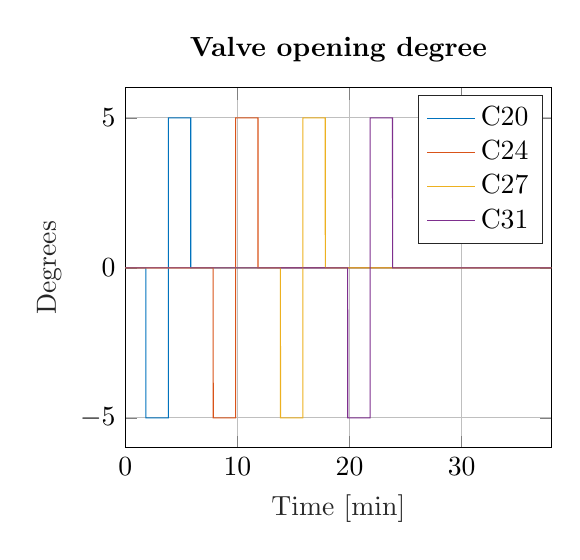
\begin{tikzpicture}

\begin{axis}[%
width=2.13in,
height=1.8in,
at={(0.758in,0.481in)},
scale only axis,
xmin=0,
xmax=38,
xlabel style={font=\color{white!15!black}},
xlabel={Time [min]},
ymin=-6,
ymax=6,
ylabel style={font=\color{white!15!black}},
ylabel={Degrees},
axis background/.style={fill=white},
title style={font=\bfseries},
title={Valve opening degree},
xmajorgrids,
ymajorgrids,
legend style={legend cell align=left, align=left, draw=white!15!black}
]
\addplot [color=mycolor1]
  table[row sep=crcr]{%
0	-4.00248723053664e-11\\
1.83416666666667	-4.00248723053664e-11\\
1.83916666666666	-5.00000000004003\\
3.83416666666667	-5.00000000004003\\
3.83916666666666	4.99999999995997\\
5.83416666666667	4.99999999995997\\
5.83916666666667	-4.00248723053664e-11\\
53.3325	-4.00248723053664e-11\\
};
\addlegendentry{C20}

\addplot [color=mycolor2]
  table[row sep=crcr]{%
0	-4.4146020172775e-11\\
7.83416666666667	-4.4146020172775e-11\\
7.83916666666667	-5.00000000004415\\
9.83416666666667	-5.00000000004415\\
9.83916666666667	4.99999999995585\\
11.8341666666667	4.99999999995585\\
11.8391666666667	-4.4146020172775e-11\\
53.3325	-4.4146020172775e-11\\
};
\addlegendentry{C24}

\addplot [color=mycolor3]
  table[row sep=crcr]{%
0	-4.74145167572715e-11\\
13.8341666666667	-4.74145167572715e-11\\
13.8391666666667	-5.00000000004742\\
15.8341666666667	-5.00000000004742\\
15.8391666666667	4.99999999995258\\
17.8341666666667	4.99999999995258\\
17.8391666666667	-4.74145167572715e-11\\
53.3325	-4.74145167572715e-11\\
};
\addlegendentry{C27}

\addplot [color=mycolor4]
  table[row sep=crcr]{%
0	-4.05933064939745e-11\\
19.8341666666667	-4.05933064939745e-11\\
19.8391666666667	-5.00000000004059\\
21.8341666666667	-5.00000000004059\\
21.8391666666667	4.99999999995941\\
23.8341666666667	4.99999999995941\\
23.8391666666667	-4.05933064939745e-11\\
53.3325	-4.05933064939745e-11\\
};
\addlegendentry{C31}

\end{axis}
\end{tikzpicture}% 
    \caption{Small-signal values of the opening degrees of the pma valves. }
    \label{fig:est_OD_data}
  \end{minipage}
  \hfill
  \begin{minipage}[b]{0.45\textwidth}
    % This file was created by matlab2tikz.
%
%The latest updates can be retrieved from
%  http://www.mathworks.com/matlabcentral/fileexchange/22022-matlab2tikz-matlab2tikz
%where you can also make suggestions and rate matlab2tikz.
%
\definecolor{mycolor1}{rgb}{0.00000,0.44700,0.74100}%
\definecolor{mycolor2}{rgb}{0.85000,0.32500,0.09800}%
%
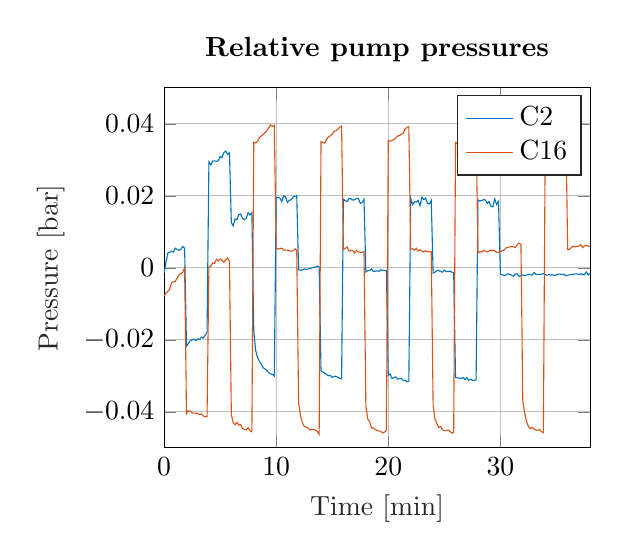
\begin{tikzpicture} 

\begin{axis}[%
scaled y ticks = false,
 y tick label style={/pgf/number format/fixed,
/pgf/number format/1000 sep = \thinspace}, % Optional if you want to replace comma as the 1000 separator 
width=2.13in,
height=1.8in,
at={(0.758in,0.481in)},
scale only axis,
xmin=0,
xmax=38,
xlabel style={font=\color{white!15!black}},
xlabel={Time [min]},
ymin=-0.05,
ymax=0.05,
ytick = {-0.04,-0.02,0,0.02,0.04},
ylabel style={font=\color{white!15!black}},
ylabel={Pressure [bar]},
axis background/.style={fill=white},
title style={font=\bfseries},
title={Relative pump pressures},
xmajorgrids,
ymajorgrids,
legend style={legend cell align=left, align=left, draw=white!15!black}
]
\addplot [color=mycolor1]
  table[row sep=crcr]{%
0	-0.00139489180470775\\
0.166666666666664	0.00145823625003061\\
0.333333333333336	0.0041219703653752\\
0.5	0.00432358326860083\\
0.666666666666664	0.0046229478824884\\
0.833333333333336	0.00441522549733975\\
1	0.00548438483264846\\
1.16666666666666	0.00510559695385382\\
1.33333333333334	0.00487343664106987\\
1.5	0.00519112970069813\\
1.66666666666666	0.00597314338593691\\
1.83333333333334	0.00545994690499896\\
2	-0.0217211381389646\\
2.16666666666666	-0.0210185477186329\\
2.33333333333334	-0.0201937676599826\\
2.5	-0.0200349211301685\\
2.66666666666666	-0.0197844323717575\\
2.83333333333334	-0.0201876581782088\\
3	-0.0197355565164301\\
3.16666666666666	-0.0198394177090009\\
3.33333333333334	-0.0192590169269877\\
3.5	-0.0194789582759611\\
3.66666666666666	-0.0186786161449746\\
3.83333333333334	-0.0179332593512314\\
4	0.0295007582440334\\
4.16666666666666	0.028602664402392\\
4.33333333333334	0.029708480629175\\
4.5	0.0297206995930068\\
4.66666666666666	0.029622947882352\\
4.83333333333334	0.0297329185568387\\
5	0.0309242675304446\\
5.16666666666666	0.0306004649889005\\
5.33333333333334	0.0320545216851684\\
5.5	0.032439419045879\\
5.66666666666666	0.0315168872765739\\
5.83333333333334	0.0319873173841003\\
6	0.0125652743733653\\
6.16666666666666	0.0116916184593876\\
6.33333333333334	0.0136161052629049\\
6.5	0.0133717259862678\\
6.66666666666666	0.0148380016460905\\
6.83333333333334	0.0149540818024931\\
7	0.0137444043831394\\
7.16666666666666	0.0134328208054271\\
7.33333333333334	0.0137627328288872\\
7.5	0.015308431753617\\
7.66666666666666	0.0147035930439401\\
7.83333333333334	0.0153328696812807\\
8	-0.0174017344242614\\
8.16666666666666	-0.0228941586666807\\
8.33333333333334	-0.0248797402893572\\
8.5	-0.0259366806608128\\
8.66666666666666	-0.0266392710811445\\
8.83333333333334	-0.0277328683440956\\
9	-0.0280688898494716\\
9.16666666666666	-0.0285209915112503\\
9.33333333333334	-0.0291624871124228\\
9.5	-0.0294374137986395\\
9.66666666666666	-0.0296084792922855\\
9.83333333333334	-0.0300666904359801\\
10	0.0194201130830365\\
10.1666666666667	0.0195545216851869\\
10.3333333333333	0.0193834561915409\\
10.5	0.0184181580488243\\
10.6666666666667	0.0199821854193019\\
10.8333333333333	0.0197561345884125\\
11	0.0181676692902712\\
11.1666666666667	0.0187969459276118\\
11.3333333333333	0.0188885881563508\\
11.5	0.0196217259862621\\
11.6666666666667	0.0199149811182266\\
11.8333333333333	0.0200738276480408\\
12	-0.000490688480972779\\
12.1666666666667	-0.00069841086611433\\
12.3333333333333	-0.000564002263963914\\
12.5	-0.000276856613915299\\
12.6666666666667	-0.000392936770317931\\
12.8333333333333	-0.000325732469242723\\
13	-0.000142448011764884\\
13.1666666666667	-3.24773372781806e-05\\
13.3333333333333	0.000138588156367803\\
13.5	0.00020579245744301\\
13.6666666666667	0.000474609661743841\\
13.8333333333333	0.000285215722350074\\
14	-0.0286004147761574\\
14.6666666666667	-0.0299811576891571\\
14.8333333333333	-0.0298834059785023\\
15	-0.0304454783147676\\
15.1666666666667	-0.0301400042189712\\
15.3333333333333	-0.0300911283636438\\
15.5	-0.0304088214232721\\
15.6666666666667	-0.030671529145657\\
15.8333333333333	-0.0307814998201437\\
16	0.0190474346861649\\
16.1666666666667	0.0186625373254614\\
16.3333333333333	0.0184609244222358\\
16.5	0.0192368286255586\\
16.6666666666667	0.0192001717340631\\
16.8333333333333	0.0188152743733596\\
17	0.0189435734935941\\
17.1666666666667	0.0193101424085498\\
17.3333333333333	0.0192857044808861\\
17.5	0.0179110710498023\\
17.6666666666667	0.0181249029168598\\
17.8333333333333	0.019035215722333\\
18	-0.001150512527893\\
18.1666666666667	-0.000765615167189537\\
18.3333333333333	-0.000771724649105465\\
18.5	-0.000313513505410867\\
18.6666666666667	-0.000991665998078872\\
18.8333333333333	-0.00093668066083552\\
19	-0.000820600504432889\\
19.1666666666667	-0.00096722807041516\\
19.3333333333333	-0.000527345372468346\\
19.5	-0.000661753974618762\\
19.6666666666667	-0.00069841086611433\\
19.8333333333333	-0.000796162576769177\\
20	-0.0298895154604182\\
20.1666666666667	-0.0295351655092944\\
20.3333333333333	-0.0307448429286481\\
20.5	-0.0304210403871039\\
20.6666666666667	-0.0303049602307013\\
20.8333333333333	-0.0309036894584622\\
21.1666666666667	-0.0307265144830779\\
21.3333333333333	-0.0312641488921628\\
21.5	-0.031233601482441\\
21.6666666666667	-0.0316307178070971\\
21.8333333333333	-0.03146576179536\\
22	0.0193712372271335\\
22.1666666666667	0.0175628305800331\\
22.3333333333333	0.0183937201206206\\
22.5	0.018289858927929\\
22.6666666666667	0.018711413180192\\
22.8333333333333	0.0172695754479975\\
23	0.0196339449495255\\
23.1666666666667	0.0189435734929546\\
23.3333333333333	0.0193956751548825\\
23.5	0.0179171805310432\\
23.6666666666667	0.0177461150374967\\
23.8333333333333	0.0187053036983613\\
24	-0.00143765817838926\\
24.1666666666667	-0.00119327890195819\\
24.3333333333333	-0.000728958276326352\\
24.5	-0.000747286722067031\\
24.6666666666667	-0.00101610392621865\\
24.8333333333333	-0.0012116073475994\\
25	-0.000643425529389674\\
25.1666666666667	-0.0010161039262897\\
25.3333333333333	-0.00103443237210854\\
25.5	-0.00092446169750815\\
25.8333333333333	-0.00139489180502039\\
26	-0.0304821352068458\\
26.1666666666667	-0.0305737774356487\\
26.3333333333333	-0.0306104343272011\\
26.5	-0.0307326239654202\\
26.6666666666667	-0.0304454783153716\\
26.8333333333333	-0.0310319885793149\\
27	-0.0305065731345238\\
27.1666666666667	-0.0312336014824908\\
27.3333333333333	-0.0310014411697779\\
27.5	-0.0312152730367785\\
27.6666666666667	-0.0312702583739508\\
27.8333333333333	-0.0311114118442362\\
28	0.0188763691920002\\
28.1666666666667	0.0185831140599433\\
28.3333333333333	0.0187114131802417\\
28.5	0.0189435734931322\\
28.6666666666667	0.0188580407461743\\
28.8333333333333	0.0179049615673108\\
29	0.0184120485664536\\
29.1666666666667	0.0171290573639737\\
29.3333333333333	0.0169579918702851\\
29.5	0.0191635148419067\\
29.6666666666667	0.0176178159172053\\
29.8333333333333	0.0185036907950433\\
30	-0.00171869434679195\\
30.3333333333333	-0.0021097011892337\\
30.5	-0.00198751155090093\\
30.6666666666667	-0.00163927108179962\\
30.8333333333333	-0.00178589864775347\\
31	-0.00203638740624257\\
31.1666666666667	-0.00235408046590635\\
31.3333333333333	-0.00169425641899323\\
31.5	-0.00168203745517559\\
31.6666666666667	-0.00236018994774412\\
31.8333333333333	-0.00210359170736751\\
32	-0.00194474517746102\\
32.1666666666667	-0.0021341391168832\\
32.3333333333333	-0.00200583999667714\\
32.5	-0.00177367968388609\\
32.6666666666667	-0.00192030724985415\\
32.8333333333333	-0.00200583999672688\\
33	-0.00130935905831819\\
33.1666666666667	-0.00185921243073039\\
33.3333333333333	-0.00181033657548113\\
33.5	-0.00183477450305247\\
33.6666666666667	-0.0017553512381312\\
33.8333333333333	-0.00156595729870901\\
34	-0.00188365035842963\\
34.1666666666667	-0.0020363874062852\\
34.3333333333333	-0.00185921243069487\\
34.5	-0.00200583999665582\\
34.6666666666667	-0.0019141977679098\\
34.8333333333333	-0.00213413911680505\\
35.1666666666667	-0.00168814693694941\\
35.3333333333333	-0.00175535123805304\\
35.5	-0.00189586932216912\\
35.6666666666667	-0.00173702279234078\\
35.8333333333333	-0.0021952339360567\\
36	-0.00203638740630652\\
36.3333333333333	-0.00182866502116497\\
36.5	-0.00182866502110102\\
36.6666666666667	-0.00165149004562437\\
36.8333333333333	-0.00170647538281798\\
37	-0.00184088398482629\\
37.1666666666667	-0.00162705211794645\\
37.3333333333333	-0.00192030724991099\\
37.5	-0.00186532191253974\\
37.6666666666667	-0.00111996511879653\\
37.8333333333333	-0.00199362103295186\\
38	-0.00154762885295412\\
38.1666666666667	-0.00174924175630053\\
38.3333333333333	-0.00155984781689966\\
38.5	-0.00148042455182917\\
38.6666666666667	-0.0021707960084143\\
38.8333333333333	-0.00124215475717193\\
39	-0.00164538056368002\\
39.1666666666667	-0.00175535123807435\\
39.3333333333333	-0.00160261419026142\\
39.5	-0.00156595729870901\\
39.6666666666667	-0.00135823491364562\\
39.8333333333333	-0.00133379698605296\\
40	-0.00146209610613113\\
40.3333333333333	-0.00126659268493512\\
40.5	-0.00121771682960059\\
40.6666666666667	-0.00129103061253488\\
40.8333333333333	-0.000625097083712944\\
41	-0.00128492113057632\\
41.1666666666667	-0.00111996511900259\\
41.3333333333333	-0.00162705211793934\\
41.5	-0.000753396203876378\\
41.8333333333333	-0.000790053095428789\\
42	-0.000551783300679176\\
42.1666666666667	-0.000967228070969384\\
42.3333333333333	-0.000942790143270145\\
42.5	-5.69152657305949e-05\\
42.6666666666667	-0.000667863457231022\\
42.8333333333333	-0.000918352215485641\\
43	-0.000295185060139147\\
43.1666666666667	-0.000466250553920133\\
43.3333333333333	-8.03941040317113e-06\\
43.5	-0.00041737469859271\\
43.6666666666667	-0.000252418686997657\\
43.8333333333333	0.000150807119624119\\
44	0.000187464011091265\\
44.1666666666667	0.000859507021942818\\
44.5	0.000468500179252374\\
44.6666666666667	0.000841178576258983\\
44.8333333333333	0.000828959612164226\\
45	0.00100613458785404\\
45.1666666666667	0.000810631166686449\\
45.3333333333333	0.00114054319011103\\
45.6666666666667	0.00200808962211596\\
45.8333333333333	0.00186146205631132\\
46	0.00167206811648413\\
46.1666666666667	0.00215471718811955\\
46.3333333333333	0.00297949724677693\\
46.5	0.0030589205116982\\
46.6666666666667	0.00295505931924822\\
46.8333333333333	0.00329108082453899\\
47	0.00370041611274985\\
47.1666666666667	0.003920357461908\\
47.3333333333333	0.00446410135237585\\
47.5	0.00480623233950439\\
47.6666666666667	0.00554547965146668\\
47.8333333333333	0.00558824602479291\\
48	0.00607089509629333\\
48.1666666666667	0.00607700457781846\\
48.3333333333333	0.00632749333657046\\
48.5	0.00648023038446155\\
48.6666666666667	0.0064435734931152\\
48.8333333333333	0.00668184328783639\\
49	0.00712172598587557\\
49.1666666666667	0.00737221474435756\\
49.3333333333333	0.00696287945559959\\
49.5	0.00737221474424388\\
49.6666666666667	0.00789763018895684\\
49.8333333333333	0.00725613458760677\\
50	0.00776933106877209\\
50.1666666666667	0.00889347574166521\\
50.3333333333333	0.00866131542857573\\
50.5	0.0086613154285331\\
50.6666666666667	0.00889347574139521\\
50.8333333333333	0.00828252754984504\\
51	0.00849024993481606\\
51.1666666666667	0.00904621278917261\\
51.3333333333333	0.00888125677727913\\
51.5	0.00915007398194234\\
51.6666666666667	0.00991375922147597\\
51.8333333333333	0.00907676019874515\\
52	0.00919894983708502\\
52.1666666666667	0.00987099284792237\\
52.3333333333333	0.00940667222214842\\
52.5	0.00986488336603486\\
52.6666666666667	0.00959606616175535\\
52.8333333333333	0.00963272305312302\\
53	0.009370015330596\\
53.1666666666667	0.0100970436786199\\
};
\addlegendentry{C2}

\addplot [color=mycolor2]
  table[row sep=crcr]{%
0	-0.00779296760428139\\
0.166666666666664	-0.00701095391904261\\
0.333333333333336	-0.00655885225725683\\
0.5	-0.00589291872842779\\
0.666666666666664	-0.00410284052708221\\
0.833333333333336	-0.00387068021427694\\
1	-0.00377903798553803\\
1.33333333333334	-0.00190342703727708\\
1.5	-0.00164682879680811\\
1.66666666666666	-0.0011641797254498\\
1.83333333333334	5.16071758198677e-05\\
2	-0.0404481484450088\\
2.16666666666666	-0.0396844632055178\\
2.33333333333334	-0.0398127623257523\\
2.5	-0.0403137398428584\\
2.83333333333334	-0.0403809441439336\\
3	-0.0404481484450088\\
3.16666666666666	-0.040771950986553\\
3.33333333333334	-0.040600885492907\\
3.5	-0.0411568483472564\\
3.66666666666666	-0.0413951181419776\\
3.83333333333334	-0.0412423810940794\\
4	0.000198234741660031\\
4.16666666666666	0.000497599355540501\\
4.33333333333334	0.00137736475143413\\
4.5	0.00124295614928371\\
4.66666666666666	0.00235488185826682\\
4.83333333333334	0.00190888967840408\\
5	0.0024587430508376\\
5.16666666666666	0.00214715947312527\\
5.33333333333334	0.00157286817302804\\
5.5	0.00231822496677125\\
5.66666666666666	0.00274588870088621\\
5.83333333333334	0.00178059055816959\\
6	-0.0407780604681847\\
6.16666666666666	-0.0430019118855824\\
6.33333333333334	-0.0435884221495115\\
6.5	-0.0428858317291798\\
6.66666666666666	-0.0436983928239982\\
6.83333333333334	-0.0434967799207726\\
7	-0.0446942383762945\\
7.16666666666666	-0.0448164280146131\\
7.33333333333334	-0.0449997124720909\\
7.5	-0.04440098324433\\
7.66666666666666	-0.0452135443391484\\
7.83333333333334	-0.0455190184349448\\
8	0.0348512161690877\\
8.16666666666666	0.0347473549765169\\
8.33333333333334	0.035083376481893\\
8.5	0.03618308322676\\
8.66666666666666	0.0365985279970431\\
8.83333333333334	0.0371056149960651\\
9	0.0375271692482642\\
9.16666666666666	0.0381625553675207\\
9.33333333333334	0.0389140216431798\\
9.5	0.0397082542922504\\
9.66666666666666	0.0392989190038833\\
9.83333333333334	0.0396166120635115\\
10	0.00558068830987679\\
10.1666666666667	0.00519579094917333\\
10.3333333333333	0.0053851848885671\\
10.5	0.00548293659922194\\
10.6666666666667	0.00490864529912471\\
10.8333333333333	0.00495752115445214\\
11.1666666666667	0.00484144099804951\\
11.3333333333333	0.0046214996490761\\
11.5	0.00473757980547873\\
11.6666666666667	0.00526910473216446\\
11.8333333333333	0.00503083493744327\\
12	-0.0373384221495172\\
12.1666666666667	-0.0410652061182333\\
12.3333333333333	-0.0429835834398347\\
12.5	-0.0439794289921309\\
12.6666666666667	-0.0442360272325999\\
12.8333333333333	-0.0444193116900777\\
13	-0.0450363693635865\\
13.1666666666667	-0.0448958512795201\\
13.3333333333333	-0.0448958512795201\\
13.5	-0.0450485883274183\\
13.6666666666667	-0.0454090477604581\\
13.8333333333333	-0.0462765941925198\\
14	0.0350650480361452\\
14.1666666666667	0.0348084497956762\\
14.3333333333333	0.0347045886031054\\
14.5	0.0356943246734858\\
14.6666666666667	0.0364213530214812\\
14.8333333333333	0.0366840607438661\\
15	0.0371850382609722\\
15.1666666666667	0.037960942464295\\
15.3333333333333	0.0380586941749499\\
15.5	0.0384924673909808\\
15.6666666666667	0.039066758691078\\
15.8333333333333	0.0393722327868744\\
16	0.00509192975660255\\
16.3333333333333	0.00578841069501834\\
16.5	0.00463982809482388\\
16.6666666666667	0.00482311255230172\\
16.8333333333333	0.00486587892571322\\
17	0.00416939798729743\\
17.1666666666667	0.00484144099804951\\
17.3333333333333	0.00446265311926197\\
17.5	0.00428547814370006\\
17.6666666666667	0.00429158762561599\\
17.8333333333333	0.00456040482991682\\
18	-0.0383587056294772\\
18.1666666666667	-0.0419510809960428\\
18.3333333333333	-0.0427086567536179\\
18.5	-0.0444865159911529\\
18.6666666666667	-0.0444865159911529\\
18.8333333333333	-0.0448530849061086\\
19	-0.0451463400380732\\
19.1666666666667	-0.0453357339774669\\
19.3333333333333	-0.0453479529412988\\
19.5	-0.0458733683860686\\
19.6666666666667	-0.0456106606639182\\
19.8333333333333	-0.045170777966284\\
20	0.0353644126494927\\
20.1666666666667	0.0351750187100919\\
20.5	0.0356149014079747\\
20.8333333333333	0.0366535133336328\\
21	0.036763484008155\\
21.1666666666667	0.0371667098146276\\
21.3333333333333	0.0373194468625115\\
21.5	0.0386085475468576\\
21.6666666666667	0.0390728681723971\\
21.8333333333333	0.0391950578107299\\
22	0.00518357198486541\\
22.1666666666667	0.00530576162303475\\
22.3333333333333	0.00492086426232419\\
22.5	0.00543406074329766\\
22.6666666666667	0.00471314187723948\\
22.8333333333333	0.00503083493688194\\
23	0.00465204705809441\\
23.1666666666667	0.00441377726330927\\
23.3333333333333	0.00476812721451125\\
23.5	0.004499310010182\\
23.8333333333333	0.00449320052823765\\
24	-0.0383037202928449\\
24.1666666666667	-0.041999956852024\\
24.3333333333333	-0.043270729090402\\
24.5	-0.0443093410162447\\
24.6666666666667	-0.0440710712213814\\
24.8333333333333	-0.0449997124726593\\
25	-0.0451463400386771\\
25.1666666666667	-0.0451891064121241\\
25.3333333333333	-0.0450546978098814\\
25.5	-0.0454273762067956\\
25.6666666666667	-0.045916134760084\\
25.8333333333333	-0.045726740820669\\
26	0.0348573256503855\\
26.1666666666667	0.0345213041450236\\
26.3333333333333	0.0350833764813174\\
26.5	0.0352177850835247\\
26.6666666666667	0.0358287332751033\\
26.8333333333333	0.0360303461782649\\
27	0.0364885573219311\\
27.1666666666667	0.0365801995507482\\
27.3333333333333	0.0373622132360154\\
27.5	0.0380892415840108\\
27.6666666666667	0.0382786355233975\\
27.8333333333333	0.0383152924147865\\
28	0.00410830316747735\\
28.1666666666667	0.00454207638357218\\
28.3333333333333	0.00435268244412867\\
28.5	0.00482311255176171\\
28.8333333333333	0.00445654363672787\\
29.1666666666667	0.0049636306357641\\
29.3333333333333	0.00476201773265217\\
29.5	0.00480478410602103\\
29.6666666666667	0.00423660228762657\\
30	0.00442599622725481\\
30.1666666666667	0.00480478410603524\\
30.3333333333333	0.00494530219003764\\
30.5	0.00557457882741375\\
30.6666666666667	0.00572731587534037\\
30.8333333333333	0.00580062965826755\\
31	0.0059900235976329\\
31.3333333333333	0.00566622105601056\\
31.5	0.00646045370515225\\
31.6666666666667	0.00687589847543535\\
31.8333333333333	0.00652765800625588\\
32	-0.0370451670181851\\
32.1666666666667	-0.0402831924335416\\
32.3333333333333	-0.0427575326094498\\
32.5	-0.0440221953662459\\
32.6666666666667	-0.0446759099311222\\
32.8333333333333	-0.0442849030883963\\
33	-0.0447675521598754\\
33.1666666666667	-0.045024150400387\\
33.3333333333333	-0.0451402305566404\\
33.5	-0.0448836323163277\\
33.6666666666667	-0.045512908953576\\
33.8333333333333	-0.0457572882302912\\
34	0.0355415876250049\\
34.1666666666667	0.0355049307336017\\
34.3333333333333	0.0363908056113331\\
34.5	0.0368245788273924\\
34.6666666666667	0.0377348916328941\\
34.8333333333333	0.0374966218381445\\
35	0.0383030734510257\\
35.3333333333333	0.0389873354254959\\
35.5	0.0400015094236679\\
35.8333333333333	0.0410034644579085\\
36	0.00507360131026502\\
36.1666666666667	0.00518968146665344\\
36.3333333333333	0.00563567364651618\\
36.5	0.00603889945294611\\
36.6666666666667	0.00584339603171458\\
36.8333333333333	0.00599002359772527\\
37	0.00602668048919242\\
37.1666666666667	0.00647267266904095\\
37.3333333333333	0.00563567364648776\\
37.5	0.00607555634453405\\
37.6666666666667	0.00630771665723984\\
37.8333333333333	0.00599613307956304\\
38	0.00604500893485493\\
38.1666666666667	0.00551959349019882\\
38.3333333333333	0.00608166582632208\\
38.5	0.00620385546475433\\
38.6666666666667	0.0059106003326832\\
38.8333333333333	0.00583728654979865\\
39	0.00536074696035627\\
39.1666666666667	0.00616108909131441\\
39.3333333333333	0.00611221323602962\\
39.5	0.00600835204337358\\
39.6666666666667	0.00610610375406395\\
39.8333333333333	0.00603278997111545\\
40	0.0056723305382107\\
40.1666666666667	0.00588005292322435\\
40.3333333333333	0.00626495028393492\\
40.5	0.00607555634439905\\
40.6666666666667	0.00633826406681948\\
40.8333333333333	0.00611832271790291\\
41	0.00652154852429732\\
41.1666666666667	0.00677203728296405\\
41.5	0.00577619173058963\\
41.6666666666667	0.0067109424641103\\
41.8333333333333	0.00570287794787561\\
42	0.00650322007854953\\
42.1666666666667	0.00656431489780829\\
42.3333333333333	0.00642379681380589\\
42.5	0.00656431489805698\\
42.6666666666667	0.00653376748818602\\
42.8333333333333	0.00602057100731912\\
43	0.00631382613914866\\
43.1666666666667	0.00608166582653524\\
43.3333333333333	0.005776191730547\\
43.5	0.00626495028388518\\
43.6666666666667	0.00639324940434705\\
43.8333333333333	0.00628327872952639\\
44	0.00598391411572408\\
44.1666666666667	0.0058556149956317\\
44.3333333333333	0.00618552701919128\\
44.5	0.00625884080206873\\
44.6666666666667	0.00590449085063938\\
44.8333333333333	0.00646045370494619\\
45	0.00630160717548733\\
45.1666666666667	0.00647878215097109\\
45.3333333333333	0.00625884080213979\\
45.5	0.00649711059668334\\
45.6666666666667	0.00569065898380217\\
45.8333333333333	0.00625884080197636\\
46	0.00630160717530259\\
46.1666666666667	0.0067475993551156\\
46.3333333333333	0.00622218391067264\\
46.5	0.00659486230747319\\
46.6666666666667	0.00632604510294499\\
46.8333333333333	0.00589838136888687\\
47	0.00602668048954769\\
47.1666666666667	0.0059716951521267\\
47.3333333333333	0.00606944686291655\\
47.6666666666667	0.0061305416817703\\
47.8333333333333	0.00588616240533923\\
48	0.00607555634449142\\
48.1666666666667	0.00605111841679928\\
48.3333333333333	0.00553181245411594\\
48.5	0.00622218391063001\\
48.6666666666667	0.0055623598637311\\
48.8333333333333	0.00589838136892951\\
49	0.00507971079236569\\
49.1666666666667	0.0052324478402852\\
49.3333333333333	0.00573342535717103\\
49.5	0.00609388479031026\\
49.6666666666667	0.0055806883092373\\
50	0.00559290727326101\\
50.1666666666667	0.00567233053804728\\
50.5	0.00520190043043556\\
50.6666666666667	0.00573342535719945\\
50.8333333333333	0.0053729659241526\\
51	0.00533630903273519\\
51.1666666666667	0.00541573229754277\\
51.3333333333333	0.00502472545510813\\
51.5	0.0054646081528702\\
51.6666666666667	0.00565400209234213\\
51.8333333333333	0.0055501408998424\\
52	0.00540351333379618\\
52.1666666666667	0.00555014089972872\\
52.3333333333333	0.00509192975619044\\
52.5	0.00549515556256353\\
52.6666666666667	0.00504305390072801\\
52.8333333333333	0.00522022887634677\\
53	0.0053363090326215\\
53.1666666666667	0.00472536084112107\\
};
\addlegendentry{C16}

\end{axis}
\end{tikzpicture}% 
    \caption{Small-signal values of the angular velocity of the two main pumps.}
    \label{fig:est_deltap_data}
  \end{minipage}
\end{figure}


\textbf{Estimation Result}


The following figures show the comparison between the data obtained from the lab and the estimated outputs of the model.  

\begin{figure}[H]
  \centering
  \begin{minipage}[b]{0.45\textwidth}
    % This file was created by matlab2tikz.
%
%The latest updates can be retrieved from
%  http://www.mathworks.com/matlabcentral/fileexchange/22022-matlab2tikz-matlab2tikz
%where you can also make suggestions and rate matlab2tikz.
%
\definecolor{mycolor1}{rgb}{0.00000,0.44700,0.74100}%
\definecolor{mycolor2}{rgb}{0.85000,0.32500,0.09800}%
%
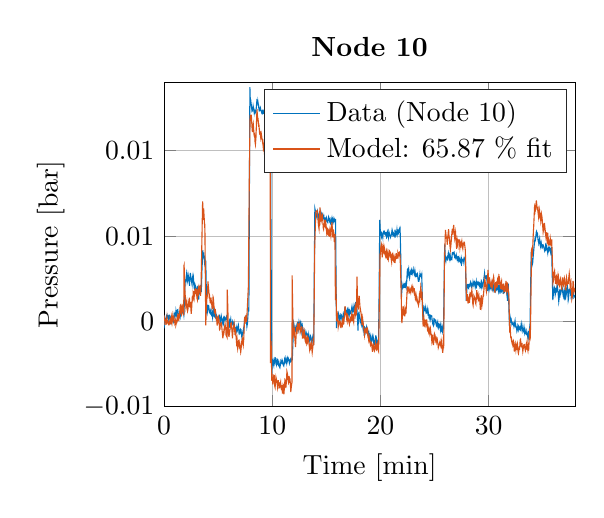
\begin{tikzpicture}

\begin{axis}[%
scaled y ticks = false,
 y tick label style={/pgf/number format/fixed,
/pgf/number format/1000 sep = \thinspace}, % Optional if you want to replace comma as the 1000 separator 
width=2.0556in,
height=1.62135in,
at={(1.011in,0.642in)},
scale only axis,
xmin=0,
xmax=38,
xlabel={Time [min]},
xmajorgrids,
ymin=-0.005,
ymax=0.014,
ylabel={Pressure [bar]},
ymajorgrids,
axis background/.style={fill=white},
title style={font=\bfseries},
title={Node 10},
legend style={legend cell align=left,align=left,draw=white!15!black}
]
\addplot [color=mycolor1,solid]
  table[row sep=crcr]{%
0.000833333333333333	-0.000410544037145466\\
0.0075	0.000346347458455742\\
0.0891666666666667	-8.95176441839673e-05\\
0.175	0.000174959384163786\\
0.1925	9.66602639290159e-05\\
0.264166666666667	0.000391586950146183\\
0.265	0.000392456940371017\\
0.296666666666667	0.000228028787879669\\
0.355833333333333	0.000295018035191275\\
0.439166666666667	6.5340615835352e-05\\
0.44	6.18606549359912e-05\\
0.481666666666667	0.000362877272727213\\
0.529166666666667	0.000348087438906269\\
0.600833333333333	9.84002443785159e-05\\
0.63	0.000158429569892649\\
0.65	-6.77678885624144e-05\\
0.703333333333333	1.05312316711348e-05\\
0.735833333333333	0.000195839149557453\\
0.85	-1.8178445749889e-05\\
0.876666666666667	0.000195839149557453\\
0.9325	0.000429866520034905\\
1.00416666666667	0.000261958406643781\\
1.0325	0.000453356256105458\\
1.07916666666667	0.000403766813292766\\
1.09916666666667	0.000589074731181388\\
1.14666666666667	0.000393326930593269\\
1.22333333333333	0.000663023900290632\\
1.26916666666667	0.000686513636360853\\
1.315	0.000375057135872991\\
1.33166666666667	0.00025847844574442\\
1.4025	0.000421166617784574\\
1.44166666666667	0.000319377761481887\\
1.47833333333333	0.000550795161288475\\
1.50583333333333	0.000362877272727213\\
1.57	0.000688253616812129\\
1.58333333333333	0.000716963294229767\\
1.62333333333333	0.000482935923748734\\
1.70583333333333	0.000686513636356578\\
1.74916666666667	0.00051338558161268\\
1.795	0.000541225268814616\\
1.83166666666667	0.000372447165201406\\
1.84	0.000431606500490789\\
1.9275	0.00218289682306369\\
1.93833333333333	0.00205326827956617\\
1.96	0.00241953416422269\\
2.015	0.00239604442814714\\
2.0825	0.00278232008797666\\
2.11	0.00260310210166215\\
2.14166666666667	0.0023003455034179\\
2.19333333333333	0.002424754105563\\
2.22666666666667	0.00272229076245842\\
2.2775	0.0025308929129978\\
2.35833333333333	0.00208284794721442\\
2.365	0.00230991539589459\\
2.43	0.00284234941348635\\
2.4525	0.00270054100683487\\
2.54	0.00232209525903221\\
2.5875	0.00216114706744086\\
2.62333333333333	0.00253176290322021\\
2.6625	0.00267531129032156\\
2.7	0.0024360639784988\\
2.71583333333333	0.00251349310850704\\
2.79166666666667	0.00195147942325852\\
2.84833333333333	0.00187927023460766\\
2.8725	0.00212721744868893\\
2.9025	0.00206109819159869\\
2.97333333333333	0.0016991822580551\\
3.0325	0.0016243630987241\\
3.05583333333333	0.00199497893450135\\
3.115	0.00204282839687486\\
3.15333333333333	0.001507784408603\\
3.19833333333333	0.00127723699902665\\
3.23833333333333	0.00177313142718069\\
3.255	0.00159217346041493\\
3.275	0.00188275019550807\\
3.32833333333333	0.00176443152493\\
3.4025	0.00213765733138238\\
3.44	0.00172354198436797\\
3.50333333333333	0.0030424471651927\\
3.58416666666667	0.00417256446724401\\
3.59083333333333	0.0040725155913848\\
3.6675	0.00380455860212128\\
3.68583333333333	0.00385936798628853\\
3.7425	0.00344699261971904\\
3.78166666666667	0.00362099066468893\\
3.84	0.00332606397848145\\
3.85416666666667	0.0035627013196376\\
3.94166666666667	0.000515995552319792\\
3.96916666666667	0.000459446187706242\\
4.01666666666667	0.000768292717523933\\
4.03916666666667	0.000692603567968381\\
4.09	0.000932720870019971\\
4.12166666666667	0.000922280987320834\\
4.2025	0.000539485288392483\\
4.25416666666667	0.000476845992217589\\
4.29166666666667	0.000607344525937553\\
4.33416666666667	0.000703043450656138\\
4.37916666666667	0.000372447165214895\\
4.44583333333333	0.000298497996099961\\
4.46416666666667	0.000404636803546105\\
4.4875	0.00024716857283813\\
4.55416666666667	0.000562105034225685\\
4.56666666666667	0.000636054203342035\\
4.64166666666667	0.000305457917903651\\
4.69416666666667	0.000259348435990653\\
4.7175	0.000410726735120243\\
4.77333333333333	0.000376797116338479\\
4.81666666666667	0.000199319110451818\\
4.83166666666667	0.000255868475073889\\
4.84166666666667	0.000128849902247957\\
4.92166666666667	0.000235858699920821\\
4.97583333333333	3.40209677589243e-05\\
4.99166666666667	9.84002443985832e-05\\
5.05583333333333	0.000241948631484995\\
5.11	0.000315027810368962\\
5.1575	9.75302541619261e-05\\
5.19666666666667	-6.95078690128026e-05\\
5.24333333333333	0.000196709139795859\\
5.28	0.000333297605105587\\
5.3375	0.000133199853387167\\
5.3425	0.000134939833839165\\
5.38666666666667	-8.34277126102179e-05\\
5.4725	0.000141899755615849\\
5.50333333333333	-9.90875366638777e-05\\
5.5175	-5.64580156477701e-05\\
5.5825	0.000241948631482164\\
5.62833333333333	0.000187139247317752\\
5.67	8.62203812233009e-05\\
5.69916666666667	0.000107970136848268\\
5.7725	0.000312417839707341\\
5.81083333333333	0.000346347458469204\\
5.8675	-0.000289615395899945\\
5.925	-0.000789859775186086\\
5.96916666666667	-0.000406194086028155\\
6.00833333333333	3.05410068577872e-05\\
6.04916666666667	8.27404203520288e-05\\
6.08583333333333	-0.000144327028340219\\
6.16333333333333	0.000134069843591128\\
6.2175	-0.000201746383197532\\
6.22416666666667	-0.000303535239501634\\
6.305	-9.82175464442903e-05\\
6.31416666666667	-0.000112137390038874\\
6.34666666666667	1.14012219001314e-05\\
6.39666666666667	-7.29878299124964e-05\\
6.46166666666667	-0.000270475610963605\\
6.48833333333333	-0.000179996627582502\\
6.56833333333333	-0.000472313343135466\\
6.62416666666667	-0.000410544037168781\\
6.63583333333333	-0.000571492228759435\\
6.65583333333333	-0.000495803079188256\\
6.71916666666667	-0.000320935044004433\\
6.75333333333333	-0.000570622238534157\\
6.83083333333333	-0.000420113929635535\\
6.8725	-0.000266125659832944\\
6.90666666666667	-0.000520162805472013\\
6.91833333333333	-0.000468833382197387\\
6.99833333333333	-0.000712430645124523\\
7.02666666666667	-0.000674151075257562\\
7.06833333333333	-0.000454913538619844\\
7.10833333333333	-0.000485363196459282\\
7.17666666666667	-0.000873378836713762\\
7.18833333333333	-0.00091252839682876\\
7.26833333333333	-0.000653271309850767\\
7.29	-0.000701990762435351\\
7.32916666666667	-0.000502763000942208\\
7.35583333333333	-0.000559312365545794\\
7.44333333333333	8.97003420917697e-05\\
7.4675	1.22712121126411e-05\\
7.55833333333333	0.000147119696974646\\
7.6175	-9.82175464130375e-05\\
7.62833333333333	-7.55978005556601e-05\\
7.6575	-0.000299185288339693\\
7.70583333333333	-0.000112137390006178\\
7.79166666666667	0.000731753128023677\\
7.83916666666667	0.000682163685202464\\
7.88166666666667	0.00673903563047282\\
7.9325	0.013733757038115\\
7.96916666666667	0.0129516358259864\\
8.0525	0.0126784588954209\\
8.05666666666667	0.0127080385630607\\
8.13	0.0123121930107417\\
8.15833333333333	0.012338292717503\\
8.23166666666667	0.0125940698436026\\
8.23416666666667	0.0126097296676435\\
8.31916666666667	0.012275653421331\\
8.3275	0.0123948420821293\\
8.39833333333333	0.0122417238025705\\
8.4125	0.0122243239980762\\
8.49416666666667	0.0124113718964126\\
8.50333333333333	0.0123765722874211\\
8.58	0.0129342360214779\\
8.58666666666667	0.0129255361192279\\
8.655	0.0127837277126006\\
8.66916666666667	0.0128898665200368\\
8.75416666666667	0.0125183806940314\\
8.76583333333333	0.0125714500977481\\
8.83583333333333	0.0123504725806428\\
8.8725	0.0123713523460126\\
8.9075	0.0124931509774897\\
8.93166666666667	0.0124235517595211\\
9.01916666666667	0.0122443337732236\\
9.06083333333333	0.0123017531280411\\
9.08833333333333	0.0121590747311743\\
9.14416666666667	0.0121747345552436\\
9.17416666666667	0.0123496025904175\\
9.19833333333333	0.0123252428641238\\
9.28	0.0121747345552408\\
9.29333333333333	0.0123174129521076\\
9.3575	0.0119494070869948\\
9.37666666666667	0.0119511470674397\\
9.43416666666667	0.0123061030791732\\
9.47	0.0123226328934564\\
9.525	0.0121390649560155\\
9.58	0.0121068753176971\\
9.6275	0.0123017531280411\\
9.63583333333333	0.0121938743401601\\
9.72	0.0123626524437797\\
9.7275	0.012371352346024\\
9.765	0.0121442848973502\\
9.82416666666667	0.0123208929129973\\
9.895	0.00410122526882198\\
9.94	-0.00311447365592835\\
10.0016666666667	-0.00251331041058189\\
10.0466666666667	-0.00233496241449552\\
10.1366666666667	-0.00257333973608093\\
10.1516666666667	-0.00240108167158293\\
10.1633333333333	-0.00244545117304962\\
10.22	-0.00224883338222662\\
10.2558333333333	-0.00238368186705451\\
10.3133333333333	-0.00216183435973244\\
10.3425	-0.00218880405670768\\
10.3925	-0.00252114032260375\\
10.4766666666667	-0.00230886270774841\\
10.5083333333333	-0.00249417062563703\\
10.5558333333333	-0.00254898000977868\\
10.5958333333333	-0.00235845215054406\\
10.5975	-0.00235410219942048\\
10.6808333333333	-0.00266816867059128\\
10.7066666666667	-0.00270992820137075\\
10.7708333333333	-0.00246633093841092\\
10.7808333333333	-0.00247329086020751\\
10.795	-0.00230973269794527\\
10.8775	-0.0024089115835991\\
10.9141666666667	-0.00226101324535499\\
10.9475	-0.00231669261974754\\
11.0091666666667	-0.00253419017594889\\
11.0641666666667	-0.00260204941351527\\
11.12	-0.0023897717986372\\
11.1208333333333	-0.00239064178886247\\
11.1466666666667	-0.00221403377320961\\
11.2083333333333	-0.00234714227762958\\
11.2516666666667	-0.00217053426197958\\
11.335	-0.00245154110463797\\
11.3775	-0.00225057336269424\\
11.3925	-0.00233496241451825\\
11.47	-0.00212964472139129\\
11.4708333333333	-0.00213051471161374\\
11.5566666666667	-0.00234279232650034\\
11.5825	-0.00244284120235672\\
11.6458333333333	-0.00224013347998517\\
11.6683333333333	-0.00221055381233123\\
11.7208333333333	-0.00236193211146224\\
11.7466666666667	-0.00235323220919237\\
11.8208333333333	-0.00214008460411175\\
11.8508333333333	-0.00227667306938736\\
11.9091666666667	-0.00128662419353839\\
11.9683333333333	-6.08079667656636e-05\\
11.9975	-0.000131277174987982\\
12.0641666666667	-0.000624561632476123\\
12.1316666666667	-0.000392274242427909\\
12.1716666666667	-0.000564532306906007\\
12.1833333333333	-0.000570622238477314\\
12.2575	-0.00029483533724739\\
12.29	-0.000395754203300624\\
12.3175	-7.29878298769693e-05\\
12.3566666666667	-6.25479472133872e-05\\
12.4141666666667	-0.000452303567955364\\
12.44	-0.000344424780074293\\
12.475	-6.68978983568436e-05\\
12.5225	-0.000267865640280668\\
12.5966666666667	-7.55978005812508e-05\\
12.6091666666667	-0.000157376881712357\\
12.6833333333333	-0.000573232209184427\\
12.7333333333333	-0.000253945796653388\\
12.7825	-0.000487103176907006\\
12.7991666666667	-0.000353994672504077\\
12.8416666666667	-0.00054713250243732\\
12.8716666666667	-0.000528862707714906\\
12.9591666666667	-0.000722870527836456\\
12.9666666666667	-0.000661971212109286\\
13.03	-0.000916878347977906\\
13.0525	-0.000848149120217495\\
13.1125	-0.000605421847502841\\
13.2025	-0.000818569452557871\\
13.2191666666667	-0.000671541104573181\\
13.2225	-0.000697640811314626\\
13.3041666666667	-0.00105781676439415\\
13.3366666666667	-0.00105346681327911\\
13.3708333333333	-0.00076898000974801\\
13.4041666666667	-0.000877728787834486\\
13.4633333333333	-0.00114916573797497\\
13.4866666666667	-0.00107521656887422\\
13.5475	-0.000864678934517776\\
13.58	-0.000925578250261988\\
13.6525	-0.00124834462364298\\
13.6666666666667	-0.00126922438902988\\
13.7425	-0.000916878347966527\\
13.75	-0.000889908651005494\\
13.8325	-0.00120745508306891\\
13.835	-0.00118918528834649\\
13.9225	0.00576377658845081\\
13.9358333333333	0.00662593690126279\\
14.015	0.00639190953076116\\
14.0875	0.00617615195497911\\
14.1291666666667	0.00607697306934232\\
14.185	0.00641191930592847\\
14.19	0.00643279907133523\\
14.2716666666667	0.00613874237533743\\
14.2766666666667	0.00615179222873372\\
14.3175	0.00592994472134911\\
14.405	0.00597779418369418\\
14.4475	0.00623531129032109\\
14.4716666666667	0.00618572184750268\\
14.485	0.00643105909091879\\
14.5541666666667	0.00628577072334202\\
14.5766666666667	0.00610394276634885\\
14.66	0.00625706104589632\\
14.6925	0.00606566319640228\\
14.765	0.00618311187675863\\
14.7983333333333	0.00598475410553626\\
14.8458333333333	0.0058733953566375\\
14.8858333333333	0.00603608352866308\\
14.8866666666667	0.00603695351888836\\
14.94	0.00590558499504118\\
15.0108333333333	0.00605435332346793\\
15.04	0.00587948528835092\\
15.1283333333333	0.00580640610943853\\
15.14	0.00594995449655336\\
15.1483333333333	0.00590471500488413\\
15.2116666666667	0.00611873260017864\\
15.2358333333333	0.0060604432550847\\
15.2983333333333	0.00587078538604124\\
15.3441666666667	0.00596735430097942\\
15.4	0.00574376681319541\\
15.4175	0.00576899652968313\\
15.4933333333333	0.00599867394911235\\
15.4983333333333	0.00593168470182809\\
15.545	0.00578117639291667\\
15.5975	0.0059934540077379\\
15.6675	0.00584816564025778\\
15.68	0.00581858597262089\\
15.7141666666667	0.00602999359723391\\
15.8216666666667	0.00584729565008366\\
15.8483333333333	0.00600650386121948\\
15.8491666666667	0.00599171402739535\\
15.9366666666667	-0.000347034750730252\\
15.9416666666667	-0.000392274242405177\\
16.0158333333333	0.000404636803578801\\
16.0258333333333	0.000415946676507462\\
16.0825	0.000212368963893594\\
16.1333333333333	0.000439436412573047\\
16.1991666666667	0.000224548826985027\\
16.2191666666667	9.6660263908227e-05\\
16.2475	0.000259348435979301\\
16.2883333333333	0.000185399266852987\\
16.345	0.000415076686293564\\
16.375	0.000386367008847865\\
16.4508333333333	7.31705279279071e-05\\
16.4616666666667	7.83904692795989e-05\\
16.5441666666667	0.000374187145705251\\
16.595	8.53503909909181e-05\\
16.6366666666667	0.000361137292274855\\
16.7175	0.000823102101723872\\
16.7558333333333	0.000820492131070744\\
16.8116666666667	0.000536005327511246\\
16.8566666666667	0.000404636803590153\\
16.8991666666667	0.000602994574863708\\
16.9516666666667	0.00070130347024111\\
16.9866666666667	0.000462926148598858\\
17.0033333333333	0.000429866520043787\\
17.0675	0.000641274144719317\\
17.075	0.000593424682328758\\
17.1183333333333	0.000384627028414353\\
17.1683333333333	0.000607344526035614\\
17.2458333333333	0.000454226246442646\\
17.2525	0.000455966226859117\\
17.3283333333333	0.000728273167276028\\
17.3675	0.00087182155436813\\
17.425	0.000615174437994942\\
17.4391666666667	0.000569934946314327\\
17.5041666666667	0.00076829271756515\\
17.5416666666667	0.000671723802558755\\
17.5616666666667	0.000850071798662144\\
17.6075	0.00067172380262695\\
17.675	0.000964040518185577\\
17.695	0.000898791251255249\\
17.7341666666667	0.00110584892471344\\
17.7791666666667	0.00111889877806426\\
17.8625	0.000374187145671168\\
17.9291666666667	-0.00053930259044388\\
17.95	2.35810850356399e-05\\
18.0066666666667	0.000569064956043586\\
18.0375	0.000401156842643552\\
18.1083333333333	7.9260459425301e-05\\
18.1275	0.000149729667673237\\
18.2125	-0.000122577272715252\\
18.2325	-0.000186956549340728\\
18.2725	1.92311339376472e-05\\
18.3141666666667	-2.07884164594718e-05\\
18.3841666666667	-0.000370524486875412\\
18.4108333333333	-0.000212186265908021\\
18.4758333333333	-0.000472313343080039\\
18.4833333333333	-0.000556702394892694\\
18.5408333333333	-0.000347034750747294\\
18.5633333333333	-0.000374874437979095\\
18.6416666666667	-0.000621081671569296\\
18.6525	-0.000568882258069392\\
18.7225	-0.000316585092919236\\
18.7575	-0.000427073851456267\\
18.8241666666667	-0.000626301612898256\\
18.8258333333333	-0.000614991739992327\\
18.8775	-0.000770719990266788\\
18.9241666666667	-0.000634131524954229\\
18.9866666666667	-0.000902958504384738\\
19.0541666666667	-0.00104215694030496\\
19.0708333333333	-0.000862068963762341\\
19.0916666666667	-0.000922098289238643\\
19.1541666666667	-0.00120832507325441\\
19.1758333333333	-0.00117526544473345\\
19.2375	-0.000880338758521698\\
19.3216666666667	-0.00110566622673924\\
19.3358333333333	-0.000925578250196624\\
19.3683333333333	-0.00102388714559676\\
19.4333333333333	-0.00131359389043406\\
19.4758333333333	-0.00136231334294756\\
19.5258333333333	-0.00109435635377075\\
19.5708333333333	-0.00081856945256642\\
19.6108333333333	-0.00115438567933235\\
19.6541666666667	-0.00130663396865452\\
19.6666666666667	-0.00109087639287531\\
19.7016666666667	-0.00119179525892854\\
19.7458333333333	-0.00136318333328656\\
19.82	-0.00131794384164005\\
19.8766666666667	0.00159739340179363\\
19.9358333333333	0.00595604442814737\\
19.99	0.00522960259047386\\
20.0383333333333	0.00506952438903319\\
20.0958333333333	0.00495207570865411\\
20.1208333333333	0.00518262311824039\\
20.1483333333333	0.00514521353857594\\
20.2166666666667	0.00491466612908062\\
20.23	0.00502689486806254\\
20.3008333333333	0.00528876192573627\\
20.3508333333333	0.00529398186708796\\
20.3858333333333	0.0051252037635138\\
20.4341666666667	0.00508344423275139\\
20.4866666666667	0.00521394276639603\\
20.5175	0.00521568274681819\\
20.57	0.00493119594330416\\
20.6025	0.00497991539587453\\
20.65	0.00522003269788776\\
20.7366666666667	0.00494163582599619\\
20.7516666666667	0.0051434735581595\\
20.7625	0.00507300434994568\\
20.7791666666667	0.00526005224830192\\
20.8466666666667	0.00512694374387912\\
20.9183333333333	0.00491640610950844\\
20.9333333333333	0.0049398958455911\\
21.015	0.00509214413490758\\
21.0758333333333	0.00536184110459181\\
21.1208333333333	0.00523308255128405\\
21.1508333333333	0.0050042751221995\\
21.2041666666667	0.00500949506357962\\
21.2266666666667	0.00513477365595214\\
21.3075	0.00500775508310061\\
21.3533333333333	0.00538359086024662\\
21.365	0.00529659183778086\\
21.4258333333333	0.00505560454549117\\
21.4991666666667	0.00521916270773637\\
21.5241666666667	0.00535923113392733\\
21.5591666666667	0.00512955371463455\\
21.62	0.00536184110458043\\
21.6391666666667	0.00536010112411281\\
21.6716666666667	0.00520959281522984\\
21.7516666666667	0.00541491050832268\\
21.7908333333333	0.00527049213100531\\
21.8191666666667	0.00534966124151173\\
21.89	0.00348788216031584\\
21.9425	0.00142339535678251\\
21.9775	0.00182707082110345\\
22.0575	0.00208893787876013\\
22.0733333333333	0.00192624970669475\\
22.1183333333333	0.00216636700881032\\
22.1833333333333	0.00219072673505002\\
22.2191666666667	0.00199497893441822\\
22.2566666666667	0.00199323895400175\\
22.3008333333333	0.00219159672528668\\
22.3733333333333	0.00199236896369689\\
22.4116666666667	0.00225249604102237\\
22.4158333333333	0.00222117639292355\\
22.4933333333333	0.00304418714571147\\
22.5183333333333	0.00306506691111827\\
22.5516666666667	0.00278319007829714\\
22.6133333333333	0.003048537096872\\
22.6783333333333	0.00260658206261019\\
22.6933333333333	0.00255003269798953\\
22.7658333333333	0.002898028787989\\
22.7941666666667	0.00294674824055938\\
22.8208333333333	0.00278493005870223\\
22.8766666666667	0.00275970034220313\\
22.895	0.00294413826990628\\
22.9408333333333	0.00280841979481897\\
23.0258333333333	0.00304592712623025\\
23.0283333333333	0.00302591735107718\\
23.1133333333333	0.00280232986327611\\
23.175	0.00299024775188036\\
23.2033333333333	0.0027666602640736\\
23.2216666666667	0.002809289785067\\
23.255	0.00262224188669938\\
23.3266666666667	0.00263268176943687\\
23.3541666666667	0.00278928000989687\\
23.4091666666667	0.00281798968734256\\
23.4608333333333	0.00255438264917279\\
23.4658333333333	0.00256569252210148\\
23.5083333333333	0.00235428489738046\\
23.565	0.00235776485830433\\
23.6416666666667	0.00273708059635147\\
23.6575	0.00261702194527946\\
23.6775	0.00278319007825167\\
23.745	0.00275970034224862\\
23.7866666666667	0.00262833181824226\\
23.8175	0.00272490073323731\\
23.9041666666667	0.000586464760554906\\
23.9325	7.31705279165551e-05\\
23.9916666666667	0.00070391344089421\\
24.0058333333333	0.000760462805526219\\
24.0316666666667	0.000647364076341778\\
24.0816666666667	0.00063518421316508\\
24.14	0.000860511681393977\\
24.1666666666667	0.000762202785999533\\
24.2258333333333	0.000483805914039737\\
24.2841666666667	0.000509035630487681\\
24.3241666666667	0.000750022922783034\\
24.3675	0.000599514613905727\\
24.4108333333333	0.000328947653933709\\
24.4308333333333	0.000498595747795649\\
24.4825	0.000261958406649443\\
24.5166666666667	0.00031241783969882\\
24.5908333333333	7.839046915456e-05\\
24.6041666666667	0.000121889980418705\\
24.625	0.000360267302021156\\
24.7375	0.000315897800645421\\
24.775	6.44706256409666e-05\\
24.7791666666667	0.000100140224854828\\
24.8425	-0.000160856842661816\\
24.8933333333333	-0.000231326050864261\\
24.9291666666667	3.2280987294131e-05\\
24.96	-3.81882209651296e-05\\
24.9741666666667	0.00013754980448516\\
25.0658333333333	6.18606549082912e-05\\
25.1275	-0.000110397409618157\\
25.1408333333333	-4.34081622997795e-05\\
25.2033333333333	-0.000225236119332756\\
25.2816666666667	-5.21080645582983e-05\\
25.3041666666667	-0.000344424780094194\\
25.3408333333333	-0.000397494183802333\\
25.3883333333333	-0.000159986852425159\\
25.4016666666667	-0.000173036705804402\\
25.45	-0.000282655474144577\\
25.49	-0.00021044628550293\\
25.5425	-0.0004844932063022\\
25.59	-0.000226106109523921\\
25.6533333333333	-0.000570622238542678\\
25.6833333333333	-0.000594111974602574\\
25.7175	-0.000400974144669358\\
25.7516666666667	-0.000589762023430696\\
25.8233333333333	-0.000389664271769119\\
25.83	-0.000434903763438355\\
25.9175	0.00374278929614752\\
25.9375	0.00451186065488832\\
26.005	0.00359576094821681\\
26.0425	0.00350876192573402\\
26.0866666666667	0.00372625948187852\\
26.1425	0.00377323895401538\\
26.1683333333333	0.00366536016616556\\
26.2025	0.00362795058648407\\
26.2641666666667	0.00396289682303042\\
26.2766666666667	0.00401074628539824\\
26.3558333333333	0.00373408939402545\\
26.4008333333333	0.00387328782990584\\
26.4316666666667	0.00368188998044594\\
26.4608333333333	0.00380020865099345\\
26.5041666666667	0.00360707082109435\\
26.5616666666667	0.00362012067451906\\
26.6183333333333	0.00385762800589054\\
26.6241666666667	0.00383587825026416\\
26.645	0.00401509623659285\\
26.7225	0.0040464158846803\\
26.7825	0.00393853709675659\\
26.82	0.00400291637335931\\
26.8583333333333	0.00379759868034035\\
26.8875	0.00385066808400303\\
26.9475	0.00373234941338729\\
27.0066666666667	0.00389764755611713\\
27.0533333333333	0.00370450972631467\\
27.0908333333333	0.00361403074295344\\
27.1366666666667	0.00376888900296854\\
27.1508333333333	0.00378280884656737\\
27.2083333333333	0.00358358108507423\\
27.245	0.00368971989250758\\
27.3075	0.00354269154452572\\
27.3641666666667	0.00348788216033291\\
27.3733333333333	0.00364535039101815\\
27.4591666666667	0.00342176290327961\\
27.4933333333333	0.00362186065493553\\
27.5116666666667	0.00352268176933854\\
27.5341666666667	0.00364709037145167\\
27.6266666666667	0.00363317052786419\\
27.6525	0.00349745205281102\\
27.6691666666667	0.00357140122193164\\
27.7366666666667	0.00373321940369215\\
27.7816666666667	0.00367580004887463\\
27.8066666666667	0.00353747160317402\\
27.8508333333333	0.003678410019505\\
27.9316666666667	0.00124765733138907\\
27.9358333333333	0.0012006778592579\\
28.01	0.00213591735084584\\
28.0691666666667	0.00216027707714239\\
28.1016666666667	0.00197235918854949\\
28.1516666666667	0.00193233963823194\\
28.1858333333333	0.00216375703806626\\
28.2366666666667	0.00217941686223502\\
28.2583333333333	0.00200976876839012\\
28.2816666666667	0.0021576671065518\\
28.3358333333333	0.00230208548373276\\
28.41	0.00207849799602264\\
28.4283333333333	0.00219594667631645\\
28.5183333333333	0.00209415782008909\\
28.5408333333333	0.00221682644174598\\
28.5491666666667	0.00215592712599891\\
28.6316666666667	0.00229425557161994\\
28.6525	0.00216810698903919\\
28.685	0.00232905518071083\\
28.7208333333333	0.00229512556188502\\
28.7983333333333	0.00203673846511809\\
28.8066666666667	0.00208719789817313\\
28.8583333333333	0.00232383523927956\\
28.8966666666667	0.00208371793736295\\
28.9783333333333	0.00228120571842827\\
28.9975	0.00230382546427427\\
29.0433333333333	0.00218028685226135\\
29.0958333333333	0.00212286749736995\\
29.1266666666667	0.00228120571825774\\
29.1766666666667	0.00224727609956835\\
29.2108333333333	0.00196365928634212\\
29.2791666666667	0.00199671891492562\\
29.3033333333333	0.00220029662753951\\
29.3325	0.0020758880253752\\
29.3633333333333	0.00228033572803815\\
29.4575	0.00204369838717047\\
29.5075	0.00227076583569077\\
29.5891666666667	0.00264747160292564\\
29.6216666666667	0.00281276974560432\\
29.6466666666667	0.00261528196457311\\
29.6958333333333	0.00255612262929936\\
29.7133333333333	0.00265530151492477\\
29.7783333333333	0.00267531129014606\\
29.8575	0.00235428489726108\\
29.9191666666667	0.0017731314271473\\
29.945	0.00191319985335531\\
30.0016666666667	0.0023029554740433\\
30.0325	0.00219420669601367\\
30.0616666666667	0.00191406984356354\\
30.1316666666667	0.00215244716527968\\
30.1933333333333	0.00192189975567636\\
30.2175	0.00188797013682779\\
30.28	0.0021541871457075\\
30.3016666666667	0.00223422624631986\\
30.38	0.0018340307427693\\
30.405	0.00179923113387168\\
30.4641666666667	0.00209937776150901\\
30.4708333333333	0.0020602282013997\\
30.525	0.00184273064513582\\
30.5766666666667	0.00177487140760924\\
30.6091666666667	0.00223596622661126\\
30.6616666666667	0.00224814608978796\\
30.6916666666667	0.00182098088953217\\
30.7475	0.00188188020519964\\
30.7741666666667	0.00203586847497808\\
30.8466666666667	0.00188797013673683\\
30.8666666666667	0.00201237873885565\\
30.9191666666667	0.00179227121211489\\
30.98	0.00214374726274263\\
30.9966666666667	0.00200889877787494\\
31.0541666666667	0.00163219301078787\\
31.135	0.00212982741937684\\
31.1658333333333	0.00178966124146746\\
31.225	0.00172093201367579\\
31.2575	0.00198105909080232\\
31.2583333333333	0.00197670913967021\\
31.3416666666667	0.00180358108496967\\
31.3525	0.00192972966755042\\
31.3916666666667	0.00166090268818242\\
31.445	0.00168787238506957\\
31.4566666666667	0.00186448040070536\\
31.5216666666667	0.00184012067438608\\
31.5583333333333	0.00208632790797628\\
31.6091666666667	0.00194364951110948\\
31.6675	0.00166003269799694\\
31.7016666666667	0.00177226143701864\\
31.735	0.00121198773215248\\
31.8116666666667	0.00221247649061387\\
31.8716666666667	0.000831802003857324\\
31.9308333333333	-0.000279175513220709\\
31.985	0.000266308357832701\\
32.0466666666667	3.31509776387851e-05\\
32.0841666666667	0.000105360166297475\\
32.1333333333333	-8.60376830601195e-05\\
32.1441666666667	-3.38382696113415e-05\\
32.2183333333333	-0.000162596823010064\\
32.2791666666667	-0.000220016177821886\\
32.3	-5.47180351432031e-05\\
32.3091666666667	-0.000108657429019776\\
32.345	-0.000282655473996779\\
32.44	3.14109972109622e-05\\
32.4716666666667	-0.000189566519851719\\
32.4858333333333	-0.000159116862017972\\
32.5716666666667	-0.000412284017512782\\
32.5858333333333	-0.000311365151414056\\
32.6183333333333	-0.000566272287348069\\
32.6766666666667	-0.000447083626524097\\
32.7075	-0.000209576295118502\\
32.7525	-0.0002617757085559\\
32.7875	-0.000510592912850383\\
32.8858333333333	-0.000343554789641543\\
32.9158333333333	-0.000472313342915198\\
32.9866666666667	-0.00054017258055547\\
32.9983333333333	-0.000366174535578467\\
33.01	-0.000408804056623024\\
33.0616666666667	-0.000141717057603269\\
33.105	-0.000327894965734238\\
33.1758333333333	-0.000616731720300773\\
33.2025	-0.000580192130907098\\
33.26	-0.00035486466268958\\
33.2725	-0.0004688333821391\\
33.3266666666667	-0.000667191153424035\\
33.3633333333333	-0.000494063098746222\\
33.4466666666667	-0.000735920381113364\\
33.5125	-0.000766370038981223\\
33.53	-0.000601071896222938\\
33.535	-0.00061499173986157\\
33.6158333333333	-0.000912528396987911\\
33.6608333333333	-0.000755060166126448\\
33.6958333333333	-0.000905568475071949\\
33.71	-0.000803779618787748\\
33.7725	-0.00046883338216186\\
33.8166666666667	-0.000611511779005924\\
33.885	0.00209937776148628\\
33.9358333333333	0.00408121549360066\\
33.9883333333333	0.00322514511230884\\
34.055	0.00339392321608192\\
34.0608333333333	0.00336086358750981\\
34.1483333333333	0.00404293592368823\\
34.1533333333333	0.0040281460898641\\
34.2358333333333	0.0046467091397617\\
34.2433333333333	0.00463800923754298\\
34.2908333333333	0.0048589867545602\\
34.3283333333333	0.00480330738015347\\
34.4108333333333	0.00525222233616068\\
34.4291666666667	0.00528006202330153\\
34.49	0.00503298479948036\\
34.5225	0.0050851842130428\\
34.5808333333333	0.00468411871937496\\
34.5916666666667	0.0048267971162759\\
34.6325	0.00459537971652116\\
34.7133333333333	0.00485376681328809\\
34.7608333333333	0.00449098088954406\\
34.79	0.00439615195501666\\
34.8483333333333	0.00464583914942843\\
34.8508333333333	0.00465105909076874\\
34.9341666666667	0.00430567297170092\\
34.94	0.0043013230205802\\
35	0.00448315097737442\\
35.0275	0.00449620083078209\\
35.1108333333333	0.00432394276640344\\
35.1883333333333	0.00411514511239239\\
35.2083333333333	0.00414472478000652\\
35.2858333333333	0.00455710014647229\\
35.2916666666667	0.00460320962844071\\
35.3266666666667	0.00427000337233358\\
35.3733333333333	0.00435091246327921\\
35.4558333333333	0.00404206593359369\\
35.4616666666667	0.00409600532748164\\
35.5258333333333	0.00428479320622591\\
35.5641666666667	0.00415603465299774\\
35.6366666666667	0.0043361226295574\\
35.6525	0.00434917248293096\\
35.7216666666667	0.00406381568916322\\
35.7383333333333	0.00401509623662696\\
35.8116666666667	0.00425695351910782\\
35.8216666666667	0.0043596123655775\\
35.8991666666667	0.00217593690127704\\
35.9333333333333	0.00124504736063363\\
36.0091666666667	0.00178444130016123\\
36.0683333333333	0.00199671891486877\\
36.0975	0.00193668958932994\\
36.1541666666667	0.00156868372432517\\
36.1808333333333	0.00165133279563043\\
36.2375	0.00198540904199127\\
36.2575	0.001684392424248\\
36.3366666666667	0.00213243738997881\\
36.3408333333333	0.00217506691098923\\
36.4241666666667	0.00165394276649386\\
36.4825	0.00117631813295566\\
36.5183333333333	0.00135640610941301\\
36.5641666666667	0.00187666026385933\\
36.6225	0.00157738362654392\\
36.685	0.00177661138807117\\
36.6941666666667	0.00173398186708346\\
36.775	0.00196539926695186\\
36.7825	0.00200628880748899\\
36.86	0.00165829271747817\\
36.875	0.00173137189641329\\
36.93	0.00148690464326229\\
36.9933333333333	0.00175921158370193\\
37.0375	0.0013303064028819\\
37.0483333333333	0.00123808743897916\\
37.125	0.00192885967747861\\
37.1325	0.00199236896391858\\
37.1691666666667	0.00157042370488944\\
37.2166666666667	0.00175573162267573\\
37.2858333333333	0.00202281862164999\\
37.3008333333333	0.00195495938413479\\
37.3558333333333	0.00123634745847176\\
37.3875	0.00133378636360112\\
37.44	0.00187492028339739\\
37.5108333333333	0.0018975400293457\\
37.5616666666667	0.00166525263931452\\
37.5925	0.00173920180838968\\
37.6125	0.00156172380256839\\
37.65	0.00171397209183943\\
37.7091666666667	0.00138511578692124\\
37.7375	0.00144079516131659\\
37.7933333333333	0.00173050190618232\\
37.8366666666667	0.00170092223853407\\
37.8825	0.00140599555228255\\
38	0.00154693396881248\\
};
\addlegendentry{Data (Node 10)};

\addplot [color=mycolor2,solid]
  table[row sep=crcr]{%
0.000833333333333333	-8.40333752050895e-05\\
0.00166666666666667	-0.00020003032940346\\
0.0175	0.000262538042596412\\
0.1325	5.13771980322813e-05\\
0.176666666666667	-0.0001781637882355\\
0.178333333333333	-0.000199642182460027\\
0.264166666666667	0.000258957562263952\\
0.305833333333333	-4.67739720638445e-05\\
0.3625	1.19913454084382e-05\\
0.410833333333333	-0.000197682364056333\\
0.4625	-0.000202003384790214\\
0.523333333333333	9.08192519179659e-06\\
0.533333333333333	-0.000157076834326651\\
0.558333333333333	0.000132388240727802\\
0.634166666666667	-5.72918506998555e-05\\
0.694166666666667	0.00024318986459759\\
0.701666666666667	0.000188590028906981\\
0.74	-3.98811553042753e-05\\
0.8025	0.000314688495517321\\
0.831666666666667	0.000110426597652642\\
0.908333333333333	0.00024290313093854\\
0.945	-7.96644477475912e-05\\
0.965	8.84747988788923e-05\\
0.995833333333333	-0.000105686598854699\\
1.05333333333333	4.12185532733222e-05\\
1.08666666666667	-0.000225399830287708\\
1.14583333333333	-5.16296838209202e-05\\
1.22	0.000239555967618776\\
1.23833333333333	9.25017680980034e-05\\
1.315	0.000296004255853056\\
1.36333333333333	4.07853303292608e-05\\
1.385	0.000318679841207877\\
1.4025	0.000188302581505724\\
1.485	0.000903120478912057\\
1.5125	0.000934601168442861\\
1.535	0.00053859973113687\\
1.60166666666667	0.000416054493402677\\
1.63333333333333	0.000739150967943542\\
1.66666666666667	0.000598659039019572\\
1.7475	0.00102854262364658\\
1.81833333333333	0.000359263332720006\\
1.83583333333333	0.00326215519756968\\
1.8525	0.00330302986832517\\
1.9275	0.00181249961048782\\
2.0125	0.000886344703067945\\
2.02166666666667	0.000812502600444469\\
2.10083333333333	0.00113922386753415\\
2.1025	0.00112210179918703\\
2.17583333333333	0.000619618409786012\\
2.19833333333333	0.000680169359263806\\
2.2725	0.00109247773098869\\
2.28833333333333	0.00104617697442996\\
2.34083333333333	0.001386824121856\\
2.40416666666667	0.000817592613178937\\
2.43833333333333	0.00114558084990408\\
2.46083333333333	0.000999641146844935\\
2.505	0.000443335192030701\\
2.54416666666667	0.000706789603491549\\
2.61416666666667	0.00149168783821756\\
2.65583333333333	0.00117531723486207\\
2.68666666666667	0.00163709258840212\\
2.76916666666667	0.00137191748981704\\
2.7925	0.00176759952019156\\
2.82166666666667	0.00145501180335938\\
2.85	0.0018762252695413\\
2.90416666666667	0.00190325100242424\\
2.96916666666667	0.00159956670488986\\
2.995	0.0019074926210289\\
3.03333333333333	0.00137842224930291\\
3.07916666666667	0.00127376209626555\\
3.12666666666667	0.00180953390465011\\
3.19	0.0019824552202399\\
3.20916666666667	0.00165850132321349\\
3.2625	0.00176664495829127\\
3.29333333333333	0.00209875212891176\\
3.37666666666667	0.00150435731260008\\
3.415	0.00206718199652599\\
3.41666666666667	0.00205200567314215\\
3.50333333333333	0.00499747284014831\\
3.5625	0.00703881325284971\\
3.6	0.00655649013037402\\
3.63666666666667	0.00620819697023749\\
3.67916666666667	0.00636922784096368\\
3.76	0.00548879942061746\\
3.77083333333333	0.00570500892071021\\
3.85333333333333	-0.00021043378547751\\
3.855	-0.000227474232685796\\
3.93916666666667	0.00151893669672371\\
3.97083333333333	0.00133595817549159\\
4.02916666666667	0.00181020585758708\\
4.055	0.00234798268856062\\
4.11833333333333	0.00192340726235491\\
4.1725	0.00145163202436893\\
4.20416666666667	0.00149521518973579\\
4.26666666666667	0.00107349214636666\\
4.29916666666667	0.00139612004656819\\
4.3625	0.00101833051660676\\
4.37916666666667	0.00113276648260568\\
4.4625	0.000703858984196382\\
4.46833333333333	0.000754298521824786\\
4.52833333333333	0.00143673412659002\\
4.55416666666667	0.00138338341623481\\
4.62916666666667	0.000718798513386723\\
4.64166666666667	0.00077919384976344\\
4.72083333333333	0.000463527480843956\\
4.73333333333333	0.00073000024563854\\
4.81666666666667	0.000118212714864095\\
4.84416666666667	0.000281665984967067\\
4.90166666666667	-0.000214455491972197\\
4.90583333333333	-0.000215234919107331\\
4.96666666666667	8.88000463345148e-05\\
4.99833333333333	-0.000113531004781061\\
5.03916666666667	0.000206316230967044\\
5.08083333333333	6.9512120830065e-05\\
5.13	-0.000483956708760164\\
5.17083333333333	-0.000450654102423314\\
5.19666666666667	-0.000138503651873737\\
5.28416666666667	-7.93905451483604e-05\\
5.3425	-0.00038222301342975\\
5.43	-0.000955813994569343\\
5.43166666666667	-0.000984312521224334\\
5.50166666666667	-0.000654613414668395\\
5.5175	-0.000770146168793629\\
5.59833333333333	-0.000310454040384296\\
5.64083333333333	-0.000149977653165196\\
5.6925	-0.000429999897875065\\
5.69666666666667	-0.000335771135066502\\
5.72666666666667	-0.000797357263783241\\
5.8325	-0.00095012296740045\\
5.83583333333333	0.00186713246082505\\
5.8675	0.00135395272836412\\
5.955	-0.000665284644052531\\
5.99166666666667	-0.000901989556723589\\
6.02333333333333	-0.0004899093283863\\
6.05166666666667	-0.000661792434234063\\
6.12916666666667	-0.000317747031005397\\
6.14083333333333	-0.00037155643691944\\
6.15666666666667	-0.000115738219256355\\
6.22416666666667	-7.18570196245192e-05\\
6.305	-0.000836466049971463\\
6.31583333333333	-0.000984016624758554\\
6.3925	-0.000419409561468985\\
6.39333333333333	-0.000428275158008407\\
6.47166666666667	-0.000130193679728492\\
6.48	-0.000208115511394076\\
6.56166666666667	-0.000800527654481106\\
6.6025	-0.000403530555778292\\
6.65583333333333	-0.000897533179959983\\
6.69833333333333	-0.00124643261353454\\
6.74666666666667	-0.00104384787718878\\
6.80916666666667	-0.00159136222399504\\
6.85166666666667	-0.00144224774533159\\
6.89	-0.00111096469231409\\
6.93416666666667	-0.00109770854249272\\
6.97166666666667	-0.00143474266513648\\
7.00666666666667	-0.00134750046924665\\
7.085	-0.00179838463711385\\
7.09333333333333	-0.00177140666128106\\
7.18	-0.00117452516510513\\
7.22916666666667	-0.00101335344562621\\
7.2675	-0.00124068869970849\\
7.3175	-0.00139998648800885\\
7.355	-0.00106941044184758\\
7.35916666666667	-0.00109608800530534\\
7.4425	0.000224165533461843\\
7.45	0.000266557413356839\\
7.47416666666667	-0.000141909914681161\\
7.565	0.000376622533899427\\
7.61583333333333	-8.86661319886332e-06\\
7.62916666666667	-9.52614818556677e-06\\
7.70583333333333	0.000914157117412023\\
7.79333333333333	0.00208050844605946\\
7.88166666666667	0.00863136110704088\\
7.95166666666667	0.0120987505690753\\
7.9775	0.0118007479151692\\
8.05416666666667	0.0120651021946311\\
8.0625	0.0121076640192066\\
8.14416666666667	0.0112116778385616\\
8.16916666666667	0.0110899853102176\\
8.2025	0.0114076706618768\\
8.245	0.0115638306467481\\
8.31916666666667	0.0109294159531507\\
8.36833333333333	0.0109745539453627\\
8.40666666666667	0.0105334068935538\\
8.445	0.010377856369212\\
8.49333333333333	0.0108106587694219\\
8.49416666666667	0.0108091586396168\\
8.58166666666667	0.0123392842570267\\
8.595	0.0123554413422817\\
8.66916666666667	0.0117422325835773\\
8.6825	0.0119309759274613\\
8.74166666666667	0.0113994782501024\\
8.75666666666667	0.011596321423542\\
8.84166666666667	0.0109437795476721\\
8.8475	0.0111513819452848\\
8.93083333333333	0.0107789635386148\\
8.95666666666667	0.0109349928494378\\
8.99916666666667	0.0106788132439608\\
9.01916666666667	0.0108562994493165\\
9.095	0.0105434977546007\\
9.115	0.0106791471913741\\
9.17166666666667	0.0101795933524523\\
9.21	0.0102968203061473\\
9.25833333333333	0.00997342877156717\\
9.32333333333333	0.0103149603736872\\
9.355	0.0100256546978392\\
9.37166666666667	0.0100854966535224\\
9.40666666666667	0.00986400619900185\\
9.48416666666667	0.0100831729198813\\
9.54416666666667	0.00969723892789078\\
9.56083333333333	0.00951568355405654\\
9.6325	0.00988728363420983\\
9.645	0.00994303189937919\\
9.72	0.0096861547355019\\
9.72583333333333	0.00961135753407531\\
9.8075	0.0100313595023302\\
9.80916666666667	0.0100702747655177\\
9.83583333333333	-0.00243943765908845\\
9.895	-0.00115204241632261\\
9.955	-0.00347343024733824\\
10	-0.00328749341546677\\
10.0575	-0.00369602419010055\\
10.0766666666667	-0.00356820265480906\\
10.145	-0.00314952375605689\\
10.1808333333333	-0.00316455037763427\\
10.2283333333333	-0.00379040782285811\\
10.2625	-0.00387510015784134\\
10.3325	-0.00333006877548602\\
10.34	-0.00326490165513146\\
10.4183333333333	-0.00349820707704494\\
10.4208333333333	-0.00346937991573637\\
10.4891666666667	-0.00385065623111405\\
10.5558333333333	-0.0034422858242735\\
10.5916666666667	-0.00371897601610269\\
10.6183333333333	-0.0035630659203007\\
10.6408333333333	-0.0038885798479421\\
10.6833333333333	-0.00386990614451879\\
10.77	-0.00358491158429147\\
10.7708333333333	-0.00359663015620444\\
10.8508333333333	-0.00402257867536505\\
10.8683333333333	-0.00373254954218997\\
10.9416666666667	-0.00417379914549208\\
10.9491666666667	-0.00422368678220762\\
11.0016666666667	-0.00369139477452061\\
11.0333333333333	-0.00372803364763319\\
11.0758333333333	-0.00426622343433252\\
11.1208333333333	-0.00389511308148927\\
11.1716666666667	-0.00342551216046137\\
11.2183333333333	-0.00347955184754119\\
11.2558333333333	-0.0039043178918901\\
11.2958333333333	-0.00362354501456564\\
11.355	-0.00293182136934173\\
11.4116666666667	-0.00309259383642066\\
11.4666666666667	-0.00348394219690266\\
11.4975	-0.00356447945452241\\
11.5583333333333	-0.00319927163477052\\
11.5966666666667	-0.00349850205611605\\
11.65	-0.00343764121158893\\
11.7166666666667	-0.0041413233916275\\
11.735	-0.0039852932788817\\
11.8183333333333	-0.00355535218611413\\
11.8216666666667	-0.0035803826201613\\
11.8358333333333	0.00269369109502078\\
11.9091666666667	9.84223385752785e-05\\
11.9533333333333	-0.00075064187569268\\
12.0375	-0.000475427532238649\\
12.0841666666667	-0.00095666389992786\\
12.155	-0.00150882182633211\\
12.1716666666667	-0.00124963649104155\\
12.2383333333333	-0.00031414229758433\\
12.2816666666667	-0.000739823122682201\\
12.3366666666667	-0.00022504512607912\\
12.4016666666667	-0.0004158858378087\\
12.4158333333333	-0.000166136105452894\\
12.4875	-0.000136183747733497\\
12.5133333333333	-0.000288094097774936\\
12.5375	-0.000196683773274132\\
12.585	-0.000633800927382877\\
12.6633333333333	-0.000444349421247432\\
12.6783333333333	-0.000598638640704837\\
12.7391666666667	-0.000296941335770988\\
12.7816666666667	-0.000746130982802583\\
12.785	-0.000698947435182601\\
12.8	-0.00100776081713189\\
12.885	-0.000657687686361566\\
12.9108333333333	-0.000989609799929789\\
12.9758333333333	-0.000662476604994464\\
13.045	-0.00114580797543833\\
13.085	-0.00121039994324425\\
13.1225	-0.000975446649355849\\
13.1516666666667	-0.00109037830429495\\
13.1958333333333	-0.0013427554255166\\
13.2316666666667	-0.0012925443956111\\
13.2633333333333	-0.00089207816926645\\
13.33	-0.000974142843446843\\
13.3966666666667	-0.00131587550002111\\
13.3991666666667	-0.00129747900491083\\
13.455	-0.00164504574623909\\
13.4916666666667	-0.00150234876455751\\
13.505	-0.00164448624503688\\
13.5725	-0.00153593515571622\\
13.6091666666667	-0.00130620151081702\\
13.6908333333333	-0.00182410253100024\\
13.7475	-0.00151978136350023\\
13.7766666666667	-0.00118699826772099\\
13.835	-0.00139363995858672\\
13.9225	0.00430111700940261\\
14.0091666666667	0.0061515555461091\\
14.01	0.00614805918452906\\
14.035	0.00643730597150471\\
14.1475	0.00650431316640959\\
14.185	0.00630743494529965\\
14.2716666666667	0.00562893939721002\\
14.3241666666667	0.00541767043790816\\
14.3591666666667	0.00582458817048214\\
14.36	0.00582143221220315\\
14.4058333333333	0.00668273715485139\\
14.4516666666667	0.00634706966090407\\
14.51	0.00583165706822226\\
14.5358333333333	0.00589729891750089\\
14.6175	0.00627483320507615\\
14.6391666666667	0.00624176847481035\\
14.7108333333333	0.00548646971997745\\
14.7425	0.00541166051264297\\
14.78	0.00568669025435971\\
14.8083333333333	0.00552488414874239\\
14.8383333333333	0.00576542554227974\\
14.8875	0.00562718978694981\\
14.9208333333333	0.00595611173413071\\
14.9733333333333	0.00564107794282431\\
15.0483333333333	0.00507218352510802\\
15.08	0.00510033825032753\\
15.1275	0.00542259296746587\\
15.1783333333333	0.00536360003282229\\
15.2275	0.00501932636060858\\
15.2683333333333	0.00500503001701828\\
15.3208333333333	0.00539050159005122\\
15.3325	0.00543793190780754\\
15.4091666666667	0.00502132650031395\\
15.4158333333333	0.00499518579142164\\
15.4983333333333	0.00564573374863894\\
15.5141666666667	0.0058153571324765\\
15.5858333333333	0.00514796784241423\\
15.5966666666667	0.00492185012762268\\
15.6441666666667	0.00538680649836581\\
15.6791666666667	0.00522364247107634\\
15.7375	0.0046543760875446\\
15.7941666666667	0.00512490565991175\\
15.8358333333333	0.00125537177616912\\
15.8491666666667	0.00317671607202658\\
15.9366666666667	0.000498082193318039\\
15.9533333333333	6.61344910309839e-07\\
16.0366666666667	0.000325354765419545\\
16.0975	-0.00032573437418128\\
16.1191666666667	-0.00024647533409116\\
16.1875	1.96429649043503e-05\\
16.245	1.45416090278783e-05\\
16.2866666666667	-0.000200874491595534\\
16.3116666666667	-0.000154188038118199\\
16.3558333333333	-0.000395729511177698\\
16.3808333333333	-0.000110532910639589\\
16.4433333333333	-0.000260611931535196\\
16.4766666666667	-0.000284250623638219\\
16.525	0.00016069226141147\\
16.5583333333333	0.000118659275390026\\
16.595	-0.000184255848641099\\
16.6366666666667	6.69207677271252e-05\\
16.715	0.000772976752353288\\
16.7325	0.000891915991891282\\
16.8116666666667	0.000296351476507614\\
16.8391666666667	0.000509189518095005\\
16.8791666666667	0.000102326340385098\\
16.925	-1.27035006902343e-05\\
16.9725	0.00036308389762278\\
16.9875	0.000337253436833946\\
17.0741666666667	-6.87247102416693e-06\\
17.13	-0.000143490980152039\\
17.1533333333333	7.89257075750555e-05\\
17.2125	0.00017204852162753\\
17.2316666666667	1.4040539287967e-05\\
17.2658333333333	6.27452669928509e-05\\
17.3133333333333	0.000351057027712695\\
17.3716666666667	2.16322001062507e-05\\
17.425	0.00041591009037146\\
17.4266666666667	0.000432720153681823\\
17.5108333333333	8.97524836854886e-06\\
17.5283333333333	-4.51766705307768e-05\\
17.5941666666667	0.000544116167302007\\
17.6	0.000539310528411158\\
17.6591666666667	0.000805836552370133\\
17.7083333333333	0.000421963807781711\\
17.7541666666667	0.000615459681684228\\
17.775	0.00056418015020112\\
17.8358333333333	0.00262548063182548\\
17.8625	0.00166903632918667\\
17.9425	0.000686891841068496\\
17.9525	0.000876024311203128\\
18.0375	0.00146167881266617\\
18.04	0.00148972360561643\\
18.1208333333333	0.00070677188877022\\
18.1408333333333	0.000743205421561922\\
18.2091666666667	0.000462404125133537\\
18.2125	0.000497443718436662\\
18.2966666666667	-0.000213047592784187\\
18.3	-0.000131290606169335\\
18.35	0.000181706522357453\\
18.3883333333333	-5.28054103034651e-05\\
18.4758333333333	-0.000484841365564209\\
18.4775	-0.000480134049498452\\
18.5325	-0.000819962495495507\\
18.5633333333333	-0.000679145693954023\\
18.6233333333333	-0.000430204470964781\\
18.6858333333333	-0.000404573417691883\\
18.705	-0.000570861894850593\\
18.7483333333333	-0.000478016566308561\\
18.8058333333333	-0.000720543789659468\\
18.8283333333333	-0.000588769377624416\\
18.9125	-0.00108977630823152\\
18.955	-0.00095581694766173\\
18.98	-0.00123042283905936\\
19.0033333333333	-0.00110176167262287\\
19.08	-0.00139314353818365\\
19.0941666666667	-0.00136893424538498\\
19.14	-0.00123264005547952\\
19.1766666666667	-0.00129200689149441\\
19.2616666666667	-0.00178351285798916\\
19.2633333333333	-0.00176263174345322\\
19.3458333333333	-0.00128722181869861\\
19.3533333333333	-0.00140219505461619\\
19.4291666666667	-0.00169655764219994\\
19.4508333333333	-0.00172422140669999\\
19.5241666666667	-0.00133107026706315\\
19.5333333333333	-0.00127318836780372\\
19.6066666666667	-0.00162101556186517\\
19.6325	-0.00165053814770188\\
19.6791666666667	-0.00134626268921153\\
19.7066666666667	-0.00129149842699798\\
19.7891666666667	-0.00170127418073854\\
19.8283333333333	-0.00176620982678671\\
19.8766666666667	0.000215074658644294\\
19.9608333333333	0.00396866076247472\\
19.9716666666667	0.00387486389090367\\
20.04	0.00437872112066667\\
20.095	0.00450540608497872\\
20.1383333333333	0.00399618911733405\\
20.1691666666667	0.00375683279075525\\
20.2133333333333	0.00428754742100276\\
20.24	0.00441247735446497\\
20.2916666666667	0.00409865817568976\\
20.3191666666667	0.00403965394584515\\
20.3566666666667	0.00432903022148566\\
20.4025	0.00417869803464896\\
20.4708333333333	0.00385027292797448\\
20.5475	0.0040824493355849\\
20.575	0.00375147499862882\\
20.6241666666667	0.00369065808916701\\
20.6475	0.00401339381837811\\
20.6708333333333	0.00393657112034508\\
20.7316666666667	0.00367245106143075\\
20.7516666666667	0.00376801638586691\\
20.7891666666667	0.00406015641559221\\
20.85	0.00392172426897864\\
20.86	0.0041006850701346\\
20.9325	0.00401319670809865\\
21.0033333333333	0.00361041454612479\\
21.0333333333333	0.00348341714061599\\
21.0783333333333	0.00392600916840107\\
21.1275	0.00397507901724718\\
21.1625	0.00362394675332997\\
21.2283333333333	0.0035390987444555\\
21.27	0.00379586733461641\\
21.3116666666667	0.00368147263383595\\
21.3541666666667	0.00341310347745409\\
21.365	0.0035819385581704\\
21.4475	0.00395679866714106\\
21.4566666666667	0.00400237166278825\\
21.4833333333333	0.00368992235507403\\
21.585	0.0037169171924626\\
21.6066666666667	0.00395850147840143\\
21.6408333333333	0.00381709762154229\\
21.7125	0.00403951305575367\\
21.7533333333333	0.00405994392258519\\
21.7975	0.00376720795979044\\
21.81	0.00391440092981107\\
21.89	0.00237928946320177\\
21.9733333333333	2.73375172518762e-06\\
21.9825	-9.94492253429183e-05\\
22.065	0.000605168068230996\\
22.115	0.000872130966327236\\
22.1508333333333	0.000580975917037575\\
22.185	0.000723135238931108\\
22.24	0.000349514208545136\\
22.245	0.000301391649235463\\
22.31	0.000634396021032037\\
22.3516666666667	0.000439892070514404\\
22.4158333333333	0.00115899982137401\\
22.4825	0.00202102493031565\\
22.5316666666667	0.00202564298559229\\
22.5433333333333	0.00179981235147815\\
22.6275	0.00192618128140366\\
22.6591666666667	0.00167806167289557\\
22.6891666666667	0.00169828197045408\\
22.745	0.00185604288920191\\
22.8	0.00169634538401828\\
22.8483333333333	0.00191181016003144\\
22.8825	0.00200040764038202\\
22.9258333333333	0.00180597529399502\\
22.9583333333333	0.00176180615974025\\
23.0016666666667	0.00200781179859288\\
23.0891666666667	0.00174231452712266\\
23.1158333333333	0.00195141100140897\\
23.2	0.00149671999244005\\
23.2108333333333	0.00157132339108923\\
23.2716666666667	0.00136132194097762\\
23.2991666666667	0.00153725168254777\\
23.37	0.0012686346638986\\
23.3883333333333	0.0013175224896144\\
23.4391666666667	0.00111404310636583\\
23.5125	0.000947266061521149\\
23.5516666666667	0.00120889510698269\\
23.5558333333333	0.00115153931735141\\
23.5975	0.00149489354313003\\
23.6425	0.00129293203427166\\
23.7266666666667	0.00201651970149005\\
23.7341666666667	0.00198107441145817\\
23.8108333333333	0.00127046656529771\\
23.8358333333333	0.00174875888295261\\
23.9041666666667	0.000529533243873973\\
23.9441666666667	-0.000298011976699963\\
24.0275	0.000117142997859393\\
24.0741666666667	-0.000246021619632683\\
24.115	-0.00029565020425569\\
24.1583333333333	0.000106932786064196\\
24.1708333333333	2.56562266276869e-05\\
24.2425	-0.000163663360478274\\
24.2716666666667	0.000111820002151422\\
24.3408333333333	-0.000419998127650683\\
24.385	-0.000305600954065734\\
24.42	-0.000558927923681876\\
24.455	-0.00064220660893518\\
24.4958333333333	-0.000464605990351622\\
24.5525	-0.000698839104677126\\
24.6025	-0.000435272744046655\\
24.6133333333333	-0.000405859266943446\\
24.6858333333333	-0.000810580040394831\\
24.6916666666667	-0.000736705975387397\\
24.7616666666667	-0.00123651010357307\\
24.8025	-0.0011333914500124\\
24.8358333333333	-0.000781058745304879\\
24.9041666666667	-0.00138469317500257\\
24.95	-0.00103462645232599\\
24.9625	-0.00113406159831019\\
24.9966666666667	-0.000723340059124147\\
25.0466666666667	-0.000804340523799981\\
25.1116666666667	-0.00114036180972196\\
25.1766666666667	-0.00101398338985182\\
25.205	-0.00120841032836607\\
25.2575	-0.00107339026203678\\
25.3041666666667	-0.00128003848949594\\
25.3058333333333	-0.00125708257102204\\
25.3475	-0.00153959724765284\\
25.3958333333333	-0.00143915242589713\\
25.48	-0.00122779508318898\\
25.5633333333333	-0.00141463168162367\\
25.5916666666667	-0.00123322263205362\\
25.6291666666667	-0.0013987514068967\\
25.6716666666667	-0.00118666961880503\\
25.7333333333333	-0.00169548097191965\\
25.7508333333333	-0.00184527650444525\\
25.8216666666667	-0.00145097891373357\\
25.8441666666667	-0.00157253505217559\\
25.9175	0.00338106458794546\\
26.005	0.00533131063408636\\
26.0058333333333	0.0053647063519433\\
26.0891666666667	0.00490144238728379\\
26.1366666666667	0.00492533563057259\\
26.1683333333333	0.0044951875175708\\
26.185	0.00461201948508789\\
26.2683333333333	0.00522263775001084\\
26.3	0.00540059611408937\\
26.35	0.0048774732732722\\
26.3566666666667	0.00495845189703367\\
26.44	0.00433221610886228\\
26.4641666666667	0.00421817595330206\\
26.5208333333333	0.00469242324661676\\
26.5333333333333	0.00463527423603317\\
26.6166666666667	0.00527410236824838\\
26.6516666666667	0.00543497394192501\\
26.6783333333333	0.00508770317481609\\
26.77	0.00565619750613974\\
26.7933333333333	0.00532730931314725\\
26.8033333333333	0.00540964155519111\\
26.8641666666667	0.00489213618132571\\
26.9391666666667	0.00520781763418209\\
26.9683333333333	0.00487546835129127\\
27.0425	0.00425283895604891\\
27.0566666666667	0.00440183526406299\\
27.0941666666667	0.00478623204494145\\
27.1675	0.00450157662096467\\
27.1908333333333	0.00478113681037683\\
27.3041666666667	0.00477261082747559\\
27.3183333333333	0.00450218252639404\\
27.3441666666667	0.00431039535248761\\
27.4041666666667	0.00462017164801826\\
27.4175	0.0046326815953906\\
27.4575	0.00447067025180316\\
27.5233333333333	0.00470111552248844\\
27.5816666666667	0.00436855888717865\\
27.6133333333333	0.00426925463578642\\
27.6641666666667	0.00459106698607403\\
27.6841666666667	0.00446453942193021\\
27.7116666666667	0.00464140103359871\\
27.76	0.00464211569639682\\
27.8433333333333	0.00417748523097663\\
27.8475	0.00419345167261296\\
27.9316666666667	0.00168976347593369\\
27.9833333333333	0.0011877661138557\\
28.0191666666667	0.00159877318663018\\
28.1008333333333	0.00104954019552144\\
28.1066666666667	0.00110343526401789\\
28.1883333333333	0.00139731525296168\\
28.2341666666667	0.00109645154355453\\
28.2641666666667	0.00146568829835455\\
28.2841666666667	0.00134519446523119\\
28.3008333333333	0.00163739842969146\\
28.3725	0.00152490751705179\\
28.4516666666667	0.00184067758461162\\
28.4566666666667	0.00178742419969257\\
28.5408333333333	0.00101112658954146\\
28.565	0.00094007336230003\\
28.625	0.00138175997968964\\
28.635	0.0013214810344479\\
28.645	0.00149504677365471\\
28.7191666666667	0.00136566668631413\\
28.8016666666667	0.00105017204742945\\
28.8191666666667	0.00102097617837444\\
28.8891666666667	0.00172155065165086\\
28.9025	0.00182633147501699\\
28.9433333333333	0.00144713086050398\\
29.0083333333333	0.00158836918513772\\
29.0408333333333	0.00130954077327558\\
29.1041666666667	0.00147366666995467\\
29.1408333333333	0.00117005117769269\\
29.1625	0.0013969629118444\\
29.2375	0.00068473483173735\\
29.245	0.00073050578835848\\
29.3125	0.00153100973833438\\
29.3375	0.00137773109054367\\
29.3833333333333	0.000938881291703712\\
29.42	0.00108977999478196\\
29.4991666666667	0.00157842852749153\\
29.5141666666667	0.00144852059915913\\
29.5941666666667	0.00215256437904584\\
29.6016666666667	0.00211570295380577\\
29.6483333333333	0.00245878191361473\\
29.6875	0.00228835813818822\\
29.7433333333333	0.00199286578810301\\
29.7925	0.00176085423134534\\
29.8525	0.0021483464428074\\
29.8575	0.00212908337951126\\
29.9441666666667	0.00302109457679795\\
29.945	0.00299662838582259\\
30.015	0.00222290229434276\\
30.0783333333333	0.00258558577739909\\
30.1175	0.00217350271077897\\
30.1358333333333	0.00231087393494245\\
30.2058333333333	0.00204170686204703\\
30.2125	0.00203449238417697\\
30.29	0.00229984790973813\\
30.3333333333333	0.00202377821766983\\
30.3833333333333	0.00232680913748126\\
30.46	0.00262968747134181\\
30.4766666666667	0.00256469573835045\\
30.5583333333333	0.00182238768631675\\
30.5816666666667	0.00167447086648016\\
30.6458333333333	0.00227470379080248\\
30.6833333333333	0.0022925275770388\\
30.7283333333333	0.00200395656928085\\
30.7483333333333	0.0020136500991001\\
30.8033333333333	0.00232705342170819\\
30.825	0.00223380804456966\\
30.8975	0.00257126883038977\\
30.9091666666667	0.00250749761619947\\
30.9383333333333	0.0021639052721181\\
31.005	0.00250442930031065\\
31.0816666666667	0.00210400125545001\\
31.1225	0.00189109179363907\\
31.1641666666667	0.00227514880049447\\
31.1958333333333	0.00236240460278829\\
31.2366666666667	0.0018919730620229\\
31.28	0.00187972206937831\\
31.32	0.002135581883927\\
31.375	0.00216947939952549\\
31.4058333333333	0.00189243326916423\\
31.4358333333333	0.00202855739082739\\
31.52	0.00172151767175654\\
31.5216666666667	0.00176023687891673\\
31.6041666666667	0.00236999613978449\\
31.6091666666667	0.00229856790248188\\
31.68	0.00172765042795586\\
31.7033333333333	0.00178159310702743\\
31.73	0.00228274915568325\\
31.7866666666667	0.00202976640524069\\
31.8716666666667	0.00148023618111821\\
31.8725	0.00148148090204725\\
31.9483333333333	-0.000650272547035257\\
32.0025	-0.000447553640098821\\
32.04	-0.000945323443597526\\
32.0475	-0.000894646599375736\\
32.1275	-0.00114502154655391\\
32.1358333333333	-0.00108650340864862\\
32.2216666666667	-0.001362956315914\\
32.23	-0.00138657858132425\\
32.2933333333333	-0.00114516561429696\\
32.3133333333333	-0.00118206897937051\\
32.3766666666667	-0.00177365465900805\\
32.3966666666667	-0.001632126918535\\
32.4633333333333	-0.00133943334696578\\
32.5183333333333	-0.00166050121439597\\
32.56	-0.00142040112368803\\
32.6016666666667	-0.00134085374908522\\
32.6233333333333	-0.00166598974743143\\
32.6783333333333	-0.00141206005491386\\
32.73	-0.00182194153650796\\
32.7533333333333	-0.00187352458210819\\
32.835	-0.00155002403354063\\
32.8658333333333	-0.00157803858511169\\
32.9191666666667	-0.00108044849253865\\
32.9483333333333	-0.00104989550158754\\
33.0091666666667	-0.00144621365230696\\
33.06	-0.00148963529831293\\
33.0758333333333	-0.00125247271192468\\
33.0983333333333	-0.00139556199575458\\
33.1591666666667	-0.00176023604682717\\
33.1925	-0.0016187959670573\\
33.2333333333333	-0.00138107888740914\\
33.3233333333333	-0.00135520940904766\\
33.3458333333333	-0.00157142085289396\\
33.3983333333333	-0.00170185540584637\\
33.4466666666667	-0.0014991302733994\\
33.4641666666667	-0.00167959398204416\\
33.5166666666667	-0.00133644623616861\\
33.55	-0.00119753940013734\\
33.5891666666667	-0.00157923006739281\\
33.635	-0.00172121732772392\\
33.6783333333333	-0.00142737428551782\\
33.7125	-0.0015169974890004\\
33.7866666666667	-0.000632890078187342\\
33.855	-0.000855009644583798\\
33.885	0.000268598383933098\\
33.9675	0.00422805527180196\\
33.9933333333333	0.00427104987651725\\
34.0166666666667	0.0037745311097665\\
34.0666666666667	0.00421719712815947\\
34.1458333333333	0.00540308956305129\\
34.1516666666667	0.00536492933107735\\
34.235	0.00656621959673549\\
34.2658333333333	0.00648587051168925\\
34.2758333333333	0.0067137403146719\\
34.3283333333333	0.00658875480706729\\
34.4108333333333	0.00707434159682569\\
34.4116666666667	0.007091069450569\\
34.4941666666667	0.00654521238037168\\
34.5075	0.00669078285396734\\
34.5666666666667	0.00638804939196803\\
34.5866666666667	0.00648062518456654\\
34.6233333333333	0.00613024637694226\\
34.7058333333333	0.00649863619547871\\
34.7458333333333	0.00615057569445326\\
34.7808333333333	0.00622757892469691\\
34.8241666666667	0.00586559310596634\\
34.8483333333333	0.00597122591686187\\
34.8858333333333	0.00627545031989139\\
34.9358333333333	0.00609850688007566\\
35.0216666666667	0.0053941529130413\\
35.0375	0.00524432770394623\\
35.1108333333333	0.00555249133707021\\
35.1266666666667	0.00575122970491113\\
35.1866666666667	0.00544895561472544\\
35.1983333333333	0.00551584606247575\\
35.2858333333333	0.00500814786160302\\
35.3275	0.00522253452936526\\
35.3733333333333	0.00484579297159949\\
35.395	0.00474560583724192\\
35.4575	0.00520128635278954\\
35.4616666666667	0.00513221729221756\\
35.525	0.00445076915581733\\
35.5641666666667	0.00469291499170621\\
35.6175	0.00447871916417262\\
35.6633333333333	0.00448762632056491\\
35.7016666666667	0.00484746939765008\\
35.7358333333333	0.00469186765549407\\
35.7958333333333	0.00441008546384907\\
35.8291666666667	0.00480630379108448\\
35.8991666666667	0.00341847853992618\\
35.9491666666667	0.00225480725394387\\
35.9866666666667	0.00236350275977426\\
36.0608333333333	0.00288209429827689\\
36.0958333333333	0.00296746146813653\\
36.1616666666667	0.00243763514723465\\
36.1783333333333	0.00219860687684191\\
36.2133333333333	0.0025619026177937\\
36.2675	0.0026485331081289\\
36.3116666666667	0.00226892048496014\\
36.3941666666667	0.00264835599277415\\
36.4241666666667	0.00236013879955723\\
36.4625	0.00252221453586019\\
36.5	0.00216900262471432\\
36.55	0.00207827122857019\\
36.5833333333333	0.00238951636951729\\
36.6466666666667	0.00250972142849503\\
36.6666666666667	0.00225538347697255\\
36.6891666666667	0.0022862662331364\\
36.76	0.00183242699360291\\
36.775	0.00208862795833435\\
36.8433333333333	0.00257547337258616\\
36.8625	0.00240723563925823\\
36.9241666666667	0.00214029780308202\\
36.9608333333333	0.0022475651717703\\
37.0083333333333	0.00252970239849406\\
37.0416666666667	0.00243329432293086\\
37.1083333333333	0.00187865487272218\\
37.1333333333333	0.00186141817111403\\
37.2033333333333	0.00254441035911563\\
37.2125	0.00250910438915679\\
37.2658333333333	0.0021672260560272\\
37.3616666666667	0.00222577830063643\\
37.3875	0.00245782261076545\\
37.4516666666667	0.00281625686831697\\
37.4783333333333	0.00265670126672905\\
37.5341666666667	0.00207068858129836\\
37.6066666666667	0.00228641790014878\\
37.6391666666667	0.00183966847616344\\
37.65	0.00190063564369758\\
37.6933333333333	0.00133602610194661\\
37.7425	0.00151948100048667\\
37.8041666666667	0.0023768339960213\\
37.8258333333333	0.00228485794628195\\
37.8966666666667	0.00172724161697134\\
38	0.0019342421762935\\
};
\addlegendentry{Model: 65.87 \% fit};
\end{axis}
\end{tikzpicture}% 
    \caption{Estimation comparison for node 10.}
  \end{minipage}
  \hfill
  \begin{minipage}[b]{0.45\textwidth}
    % This file was created by matlab2tikz.
%
%The latest updates can be retrieved from
%  http://www.mathworks.com/matlabcentral/fileexchange/22022-matlab2tikz-matlab2tikz
%where you can also make suggestions and rate matlab2tikz.
%
\definecolor{mycolor1}{rgb}{0.00000,0.44700,0.74100}%
\definecolor{mycolor2}{rgb}{0.85000,0.32500,0.09800}%
%
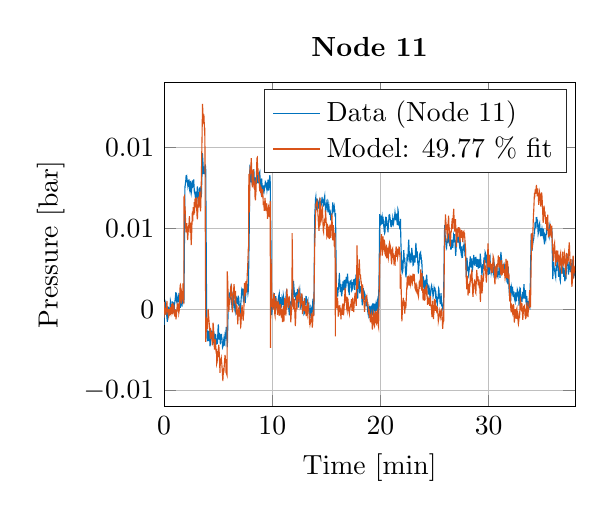
\begin{tikzpicture}

\begin{axis}[%
scaled y ticks = false,
 y tick label style={/pgf/number format/fixed,
/pgf/number format/1000 sep = \thinspace}, % Optional if you want to replace comma as the 1000 separator 
width=2.0556in,
height=1.62135in,
at={(1.011in,0.642in)},
scale only axis,
xmin=0,
xmax=38,
xlabel={Time [min]},
xmajorgrids,
ymin=-0.006,
ymax=0.014,
ylabel={Pressure [bar]},
ymajorgrids,
axis background/.style={fill=white},
title style={font=\bfseries},
title={Node 11},
legend style={legend cell align=left,align=left,draw=white!15!black}
]
\addplot [color=mycolor1,solid]
  table[row sep=crcr]{%
0.000833333333333333	-0.00095383988269801\\
0.00916666666666667	0.000151917693059583\\
0.09	-8.47196480935342e-05\\
0.13	0.000384205083089034\\
0.180833333333333	0.000238046725317048\\
0.264166666666667	-0.000527544672531327\\
0.304166666666667	-0.000759832062560556\\
0.350833333333333	-5.2530009775037e-05\\
0.3825	0.000171927468231248\\
0.434166666666667	-0.000395306158357617\\
0.480833333333333	-0.000334406842619622\\
0.519166666666667	0.000117988074292474\\
0.535	-0.000177808602149693\\
0.585833333333333	0.000546893255131881\\
0.626666666666667	0.000421614662755809\\
0.649166666666667	-7.42797653964511e-05\\
0.740833333333333	-0.000104729423265532\\
0.77	0.000461634213097861\\
0.820833333333333	0.000445974389052001\\
0.854166666666667	-0.000138659042036304\\
0.924166666666667	-0.000175198631476498\\
0.964166666666667	0.000420744672534612\\
0.971666666666667	0.000323305767353732\\
1.0325	0.000669561876831926\\
1.08833333333333	0.00106018748777539\\
1.1325	0.00055820312805363\\
1.16166666666667	0.00049295386119258\\
1.18833333333333	0.00083660000000027\\
1.245	0.000691311632451924\\
1.2925	0.000463374193545057\\
1.315	0.00048338396871625\\
1.375	0.00102190791788676\\
1.42	0.000681741739978425\\
1.4675	0.000281546236560404\\
1.49916666666667	0.00010145826001956\\
1.57333333333333	0.00087400957966613\\
1.57916666666667	0.000877489540565463\\
1.6575	0.00018236735092611\\
1.66583333333333	0.000243266666663938\\
1.73333333333333	0.000999288172042562\\
1.755	0.00100102815249098\\
1.81583333333333	0.000417264711623871\\
1.84	0.000611272531764628\\
1.9275	0.00761208387095852\\
1.93666666666667	0.0075459646138761\\
2.015	0.00801923929618911\\
2.04	0.00828632629521028\\
2.07333333333333	0.00785742111436821\\
2.11666666666667	0.00807578866079486\\
2.19	0.00766515327467945\\
2.2325	0.00797747976538976\\
2.25333333333333	0.00757119433039297\\
2.3	0.00802358924730914\\
2.36166666666667	0.00737196656891331\\
2.38	0.00731715718474962\\
2.45166666666667	0.00792963030302407\\
2.4525	0.00789483069403052\\
2.51916666666667	0.00721710830889397\\
2.54	0.00731889716520021\\
2.6225	0.0079609499511179\\
2.63333333333333	0.00750420508308383\\
2.71333333333333	0.00786090107526083\\
2.73916666666667	0.00802793919843273\\
2.80333333333333	0.00716751886607983\\
2.8225	0.00728496754642624\\
2.885	0.0069752510263861\\
2.92166666666667	0.00682735268816476\\
2.94833333333333	0.00726234780058665\\
2.9875	0.00675166353861417\\
3.06583333333333	0.00744156578690183\\
3.075	0.00759381407624393\\
3.15333333333333	0.00673861368524417\\
3.19666666666667	0.0064480369501482\\
3.23916666666667	0.00735456676441618\\
3.27916666666667	0.00752160488758666\\
3.32333333333333	0.00669163421309596\\
3.3475	0.00680908289344306\\
3.405	0.00760860391006307\\
3.4475	0.00693697145649355\\
3.50166666666667	0.00828980625610715\\
3.50333333333333	0.00828545630498215\\
3.5425	0.00963568113391491\\
3.59083333333333	0.00914500664710974\\
3.63833333333333	0.00834461564027511\\
3.6875	0.00881876031280346\\
3.76583333333333	0.00839333509286394\\
3.7675	0.00833939569892625\\
3.81333333333333	0.00894403890517598\\
3.85333333333333	0.00860387272726162\\
3.94166666666667	-0.00118090733138271\\
3.955	-0.0011052181818243\\
4.00416666666667	-0.00195780860215816\\
4.06333333333333	-0.00132358572825805\\
4.10583333333333	-0.00195258866081213\\
4.11916666666667	-0.00181426021506464\\
4.18083333333333	-0.00130444594331602\\
4.205	-0.00171421133921396\\
4.2525	-0.00226839511242499\\
4.29916666666667	-0.00193953880743433\\
4.36166666666667	-0.00135229540566112\\
4.42916666666667	-0.00143581446724991\\
4.46083333333333	-0.0018542797654035\\
4.47833333333333	-0.00186558963831654\\
4.5025	-0.00148540391007113\\
4.61583333333333	-0.00216573626587999\\
4.64	-0.00173596109480623\\
4.65916666666667	-0.00165853196480295\\
4.68583333333333	-0.00203262776147706\\
4.76416666666667	-0.00150454369501457\\
4.81666666666667	-0.00210222697947696\\
4.825	-0.00216921622679248\\
4.85916666666667	-0.00178294056697009\\
4.9275	-0.00213963655913996\\
4.99083333333333	-0.00116698748777819\\
5.01833333333333	-0.000914690322571188\\
5.07416666666667	-0.00178903049853996\\
5.08333333333333	-0.00185862971651996\\
5.13083333333333	-0.00146017419353367\\
5.20333333333333	-0.00214398651025502\\
5.25083333333333	-0.00156109305962954\\
5.31083333333333	-0.00154282326491992\\
5.33916666666667	-0.00183253000978137\\
5.34916666666667	-0.0017768506353931\\
5.40583333333333	-0.00234321427174816\\
5.46666666666667	-0.00223794545453582\\
5.51	-0.0018734195503384\\
5.53	-0.00178381055719254\\
5.59333333333333	-0.00217878611926489\\
5.61333333333333	-0.00219444594330437\\
5.64833333333333	-0.0015576130987156\\
5.6925	-0.00164635210164615\\
5.7475	-0.00107302854349167\\
5.7825	-0.0013975348973673\\
5.85	-0.00232842443793113\\
5.8675	-0.00171421133920258\\
5.93416666666667	0.00034244555229182\\
5.9675	0.000240656695986302\\
6.00583333333333	0.000950568719447681\\
6.095	0.000782660606056168\\
6.13	0.00116197634407772\\
6.15333333333333	0.00127159511240368\\
6.21583333333333	0.000585172825033481\\
6.2175	0.000636502248296755\\
6.26666666666667	0.00022760684262127\\
6.3175	0.000429444574776061\\
6.38166666666667	0.00109237712610058\\
6.395	0.000916639100681543\\
6.45833333333333	6.40486803462625e-05\\
6.49333333333333	0.000558203128052576\\
6.55	-6.12299120248405e-05\\
6.5775	-0.00014300899316308\\
6.63666666666667	0.0005590731182821\\
6.65833333333333	0.000384205083088368\\
6.6975	0.000726111241434096\\
6.74333333333333	0.000659121994131373\\
6.80416666666667	0.000313735874873128\\
6.8625	0.000846169892460613\\
6.88916666666667	0.000466854154429125\\
6.91916666666667	0.000544283284445196\\
7.00583333333333	-0.000256107722388738\\
7.03583333333333	-0.000403136070390497\\
7.09166666666667	0.00038768504397671\\
7.09416666666667	0.000345925513187267\\
7.17833333333333	0.00117763616814134\\
7.24166666666667	0.00099406823069903\\
7.24666666666667	0.00124984535680003\\
7.26833333333333	0.00123766549364607\\
7.34666666666667	0.000441624437922922\\
7.3575	0.000521663538607747\\
7.41916666666667	0.00132205454545589\\
7.44333333333333	0.00108628719452786\\
7.50583333333333	0.00040160488757271\\
7.53083333333333	0.000740031085037202\\
7.61666666666667	0.00143863323559404\\
7.66916666666667	0.00149779257088486\\
7.705	0.00119677595308479\\
7.71083333333333	0.00126028523948921\\
7.7525	0.000982758357777447\\
7.79333333333333	0.00118111612905242\\
7.88166666666667	0.00530051984360685\\
7.92916666666667	0.00893011906158284\\
7.9975	0.0078539411534877\\
8.055	0.00864476226782931\\
8.05666666666667	0.00859169286411832\\
8.13916666666667	0.00772344261978622\\
8.19333333333333	0.00768951300100587\\
8.22833333333333	0.00836723538612039\\
8.255	0.00807752864124045\\
8.29833333333333	0.00866042209188725\\
8.32333333333333	0.00820715718478485\\
8.385	0.00753639472142145\\
8.42	0.00813929794722984\\
8.47916666666667	0.0077538922776427\\
8.52	0.00777303206256197\\
8.57666666666667	0.0086134426197646\\
8.58166666666667	0.00853601348975136\\
8.65583333333333	0.00782349149561415\\
8.67083333333333	0.00782523147606473\\
8.73333333333333	0.00814973782993325\\
8.76416666666667	0.00799487956989256\\
8.84416666666667	0.00846815425222761\\
8.84833333333333	0.00847772414470574\\
8.91916666666667	0.00735804672531518\\
8.94	0.00728148758551303\\
9.00666666666667	0.00803837908113966\\
9.02333333333333	0.0080453390029476\\
9.10666666666667	0.00716838885629731\\
9.19	0.00764862346041473\\
9.195	0.00757902424242904\\
9.24333333333333	0.00727104770282669\\
9.30166666666667	0.00751029501463168\\
9.36083333333333	0.00787047096773966\\
9.38083333333333	0.00784263128054197\\
9.44833333333333	0.00759207409578838\\
9.46916666666667	0.00782697145651529\\
9.51666666666667	0.0073919763441069\\
9.54916666666667	0.00755553450637197\\
9.6075	0.00800009951124142\\
9.64833333333333	0.00733194701857659\\
9.72	0.00784089130009993\\
9.77583333333333	0.0082837163244989\\
9.8075	0.00799922952100476\\
9.895	0.00339872121211049\\
9.94083333333333	-0.000345716715551669\\
10.0208333333333	0.000158007624622813\\
10.0383333333333	0.000559073118245157\\
10.0916666666667	6.14387096704028e-05\\
10.15	0.000716541348984412\\
10.18	0.00100102815248423\\
10.2433333333333	1.09792766494754e-05\\
10.2633333333333	-8.3849657838142e-05\\
10.3266666666667	0.000821810166186793\\
10.3333333333333	0.00067826177908617\\
10.3883333333333	7.62285434888488e-05\\
10.4658333333333	0.000499913782999822\\
10.4916666666667	-7.601974583335e-05\\
10.51	0.000221516911057096\\
10.5666666666667	0.00073916109482472\\
10.6458333333333	0.000992328250225716\\
10.6833333333333	0.000311995894406919\\
10.7283333333333	0.000194547214061952\\
10.7675	0.000760910850451102\\
10.7708333333333	0.000695661583588997\\
10.8441666666667	0.000160617595278773\\
10.8641666666667	0.000175407429105739\\
10.9033333333333	0.000643462170046433\\
10.9866666666667	0.000291116129025715\\
11.0233333333333	0.000871399608993823\\
11.0391666666667	0.000807020332351305\\
11.1016666666667	8.40584555192314e-05\\
11.1758333333333	2.92490713548477e-05\\
11.2083333333333	0.000408564809376372\\
11.2325	0.000251096578682608\\
11.2908333333333	0.00106105747800886\\
11.3158333333333	0.00112108680352496\\
11.3741666666667	0.000403344868027539\\
11.4308333333333	0.00072176129030202\\
11.4658333333333	4.31689149451575e-05\\
11.4991666666667	0.000297206060571431\\
11.5408333333333	-6.12299120546778e-05\\
11.5816666666667	-0.000365726490724638\\
11.6333333333333	0.000474684066466613\\
11.6641666666667	0.000451194330403887\\
11.7166666666667	-6.81898338427411e-05\\
11.735	9.18883675354032e-05\\
11.8108333333333	0.00108802717495851\\
11.8291666666667	0.00105061759529979\\
11.8716666666667	0.00031721583576716\\
11.9275	0.000671301857292445\\
11.965	0.00176400957966796\\
11.9966666666667	0.00141862346037275\\
12.0816666666667	0.000767870772216434\\
12.1083333333333	0.00101581798627709\\
12.1691666666667	0.000662601955031095\\
12.18	0.000546893255145203\\
12.2091666666667	0.001072367350929\\
12.29	0.000690441642225925\\
12.3283333333333	0.00126376520042018\\
12.355	0.000929688954076413\\
12.4033333333333	0.00012059804496406\\
12.4366666666667	0.000258926490684569\\
12.4891666666667	0.000950568719426365\\
12.5441666666667	0.00120808582597368\\
12.6091666666667	0.000486863929612058\\
12.6433333333333	4.88934505260552e-06\\
12.6966666666667	0.000550373216017919\\
12.7016666666667	0.000574732942314471\\
12.7366666666667	0.000198897165199746\\
12.8008333333333	0.000618232453555884\\
12.8716666666667	0.000221516911017294\\
12.8775	0.000354625415417364\\
12.9325	-0.000291777321623915\\
12.96	-0.000255237732179087\\
13.04	0.000447714369482849\\
13.05	0.000280676246319472\\
13.1183333333333	0.000800930400774336\\
13.1391666666667	0.000797450439870367\\
13.2066666666667	0.000308515933525683\\
13.2908333333333	0.000537323362652886\\
13.3083333333333	0.000194547214053431\\
13.345	0.000421614662730052\\
13.3741666666667	6.31786900953946e-05\\
13.4016666666667	0.000178887390009708\\
13.485	-0.000433585728254082\\
13.4991666666667	-0.000446635581630467\\
13.57	0.000136257869004952\\
13.585	9.97182795516027e-05\\
13.6533333333333	-0.000565824242423185\\
13.6675	-0.000444025610948945\\
13.7466666666667	0.000523403519034155\\
13.7725	0.000668691886608064\\
13.835	-0.000247407820120282\\
13.8458333333333	-0.000255237732159186\\
13.9225	0.00569549540567496\\
13.9966666666667	0.00680473294231948\\
14.03	0.00695785122186696\\
14.0816666666667	0.00635842795697389\\
14.1166666666667	0.00611309071358054\\
14.1708333333333	0.00682039276639448\\
14.185	0.00670207409580431\\
14.2325	0.00624532922776955\\
14.2858333333333	0.00626794897361552\\
14.3	0.00657331554252782\\
14.3758333333333	0.00675688347996586\\
14.4366666666667	0.00610178084068028\\
14.4558333333333	0.00605828132945024\\
14.4941666666667	0.00656809560117327\\
14.5358333333333	0.00651067624629323\\
14.6091666666667	0.00694132140764059\\
14.6341666666667	0.00655591573804207\\
14.6591666666667	0.00680995288368255\\
14.725	0.006354078005856\\
14.7625	0.00669163421312366\\
14.85	0.00701266060604558\\
14.8783333333333	0.00646021681327799\\
14.8883333333333	0.00660289521014482\\
14.9275	0.0059791122189751\\
15.0175	0.00641062737046813\\
15.0608333333333	0.00673687370476447\\
15.0616666666667	0.00673774369498975\\
15.1483333333333	0.005989552101687\\
15.2216666666667	0.00646282678397941\\
15.2383333333333	0.00636625786900996\\
15.3025	0.00583817380251336\\
15.3458333333333	0.00614963030301116\\
15.4041666666667	0.00552758729227779\\
15.4175	0.00552845728251444\\
15.4891666666667	0.00589820312807493\\
15.505	0.00573464496579848\\
15.5841666666667	0.0064810965786791\\
15.595	0.00660289521016755\\
15.6458333333333	0.00611657067450441\\
15.7283333333333	0.00635755796669746\\
15.7616666666667	0.00600173196481255\\
15.7716666666667	0.00617051006842079\\
15.8125	0.00569897536653347\\
15.8491666666667	0.00594779257080522\\
15.9366666666667	0.000632152297163235\\
15.945	0.000493823851428515\\
15.9808333333333	0.00135337419355328\\
16.0508333333333	0.000810500293255273\\
16.0975	0.00129508484842522\\
16.1116666666667	0.00120808582596513\\
16.1991666666667	0.00215724516131677\\
16.2025	0.00225120410559046\\
16.2858333333333	0.00110977693057071\\
16.2908333333333	0.00106801739978554\\
16.3466666666667	0.00157174173992305\\
16.3741666666667	0.0011480565004604\\
16.415	0.000813110263908401\\
16.4616666666667	0.00108802717495568\\
16.5425	0.00173007996082791\\
16.5566666666667	0.00156913176923584\\
16.615	0.0011872060605356\\
16.65	0.00181881896380109\\
16.7083333333333	0.00128638494624059\\
16.7325	0.00126115522973583\\
16.7783333333333	0.00166048074290193\\
16.8175	0.00155173196476999\\
16.8441666666667	0.00201456676442152\\
16.9325	0.00161263128053979\\
16.9541666666667	0.00221466451606606\\
16.9908333333333	0.00185274858254164\\
17.0375	0.00132118455520075\\
17.0766666666667	0.00146647292276048\\
17.115	0.00089053939390174\\
17.1625	0.00136294408598592\\
17.1991666666667	0.00171355014659871\\
17.2875	0.00178227937444153\\
17.3366666666667	0.00123418553279184\\
17.3383333333333	0.00123853548391256\\
17.3591666666667	0.00168919042034762\\
17.4366666666667	0.00137338396871203\\
17.5116666666667	0.00181794897357013\\
17.5716666666667	0.00184317869013176\\
17.595	0.00132205454543172\\
17.6191666666667	0.00120634584552595\\
17.6683333333333	0.0018858082111706\\
17.6975	0.00175791964812225\\
17.7358333333333	0.0020415364614394\\
17.8116666666667	0.001922347800587\\
17.8608333333333	0.00126202521994973\\
17.8941666666667	0.00067826177908617\\
17.95	0.0015099724339962\\
17.9933333333333	0.00201630674484934\\
18.0383333333333	0.00170833020525268\\
18.09	0.000993198240445331\\
18.1491666666667	0.00143776324532044\\
18.1675	0.00110716695990054\\
18.22	0.00132988445751042\\
18.2966666666667	0.000485123949187066\\
18.3241666666667	0.000254576539595097\\
18.3766666666667	0.000867919648061433\\
18.4216666666667	0.00131248465294223\\
18.4716666666667	0.000639112218982552\\
18.4816666666667	0.000579952883686063\\
18.5283333333333	0.0010288678396535\\
18.5708333333333	0.000937518866055642\\
18.6508333333333	0.000383335092846021\\
18.6591666666667	0.000198027174940357\\
18.7383333333333	0.000712191397843787\\
18.7408333333333	0.00074438103617358\\
18.8233333333333	-0.000109079374419674\\
18.8725	-0.000315267057646867\\
18.9133333333333	1.96791789108253e-05\\
18.9358333333333	0.000111898142705541\\
18.985	-0.000127349169167651\\
19.0316666666667	0.000215426979417593\\
19.0658333333333	-0.000415315933525978\\
19.0966666666667	-0.000317877028351149\\
19.175	0.000164967546419398\\
19.2233333333333	0.000245006647139723\\
19.2558333333333	-0.00017606862169825\\
19.2966666666667	-0.000363986510325237\\
19.3366666666667	0.000378115151437486\\
19.4208333333333	-5.25300097933279e-05\\
19.4383333333333	0.000325915738011467\\
19.4441666666667	0.000363325317675883\\
19.4783333333333	-8.12396871878729e-05\\
19.5725	0.000313735874857501\\
19.6041666666667	-7.86297165404626e-05\\
19.6133333333333	-3.42602150623927e-05\\
19.6975	0.000445104398852481\\
19.7241666666667	0.000539933333323056\\
19.7525	-9.42895405671162e-05\\
19.8058333333333	-0.000406616031250417\\
19.8766666666667	0.00231906334311138\\
19.9325	0.00588602326492951\\
19.9791666666667	0.00517263128053291\\
20.0291666666667	0.00578336441837454\\
20.075	0.00524136050829616\\
20.1325	0.00564242600194123\\
20.1525	0.00572768504396212\\
20.2008333333333	0.00527268015637222\\
20.2316666666667	0.00571985513194026\\
20.3141666666667	0.00510303206247617\\
20.3316666666667	0.00519699100676124\\
20.3908333333333	0.00471762639293163\\
20.4158333333333	0.00476982580642019\\
20.4883333333333	0.00568418553273778\\
20.4991666666667	0.00568244555228151\\
20.565	0.0051569714564437\\
20.59	0.00537446901266211\\
20.6625	0.00498645337245879\\
20.705	0.00476025591393639\\
20.7508333333333	0.00554063714561726\\
20.7641666666667	0.00535010928639967\\
20.795	0.00581990400780233\\
20.8491666666667	0.00584600371451532\\
20.9208333333333	0.00548669775168381\\
20.9266666666667	0.00552410733134825\\
20.9666666666667	0.00507780234596569\\
21.0333333333333	0.00550496754640908\\
21.0625	0.00518742111440251\\
21.1141666666667	0.0052578903225822\\
21.1408333333333	0.00560936637342596\\
21.2091666666667	0.00530834975562589\\
21.2758333333333	0.00559979648090805\\
21.2825	0.00554585708697464\\
21.345	0.00598520215052081\\
21.385	0.00577379452586801\\
21.4208333333333	0.00550235757571618\\
21.4633333333333	0.00590255307917009\\
21.5358333333333	0.00537620899312974\\
21.5616666666667	0.00520917087002321\\
21.6183333333333	0.00616790009777904\\
21.6366666666667	0.00611657067448737\\
21.7016666666667	0.00514827155422498\\
21.7508333333333	0.00541535855323905\\
21.7875	0.00494382385140288\\
21.8491666666667	0.00559109657864956\\
21.89	0.00415909266857856\\
21.9625	0.00266357947209034\\
21.9841666666667	0.00274535855321578\\
22.0166666666667	0.00227121388072651\\
22.0725	0.00239040254152204\\
22.1525	0.00362230869978367\\
22.1558333333333	0.00366667820125602\\
22.22	0.00293762639292941\\
22.2441666666667	0.00317078377319152\\
22.3283333333333	0.00219204477029397\\
22.3675	0.00197976715549547\\
22.4133333333333	0.00263486979477537\\
22.4233333333333	0.0026052901271385\\
22.4608333333333	0.00325082287390618\\
22.5333333333333	0.00309944457472403\\
22.5891666666667	0.00408862346039887\\
22.6175	0.00430612101664568\\
22.6758333333333	0.00313076422285694\\
22.7083333333333	0.00302810537628492\\
22.7333333333333	0.00339176129028265\\
22.7683333333333	0.00329519237533307\\
22.8208333333333	0.002899346823034\\
22.8566666666667	0.00317774369498242\\
22.8916666666667	0.00380239667641721\\
22.9416666666667	0.00346397047890723\\
23.0141666666667	0.0027253487780968\\
23.065	0.00277406823070128\\
23.0966666666667	0.0033143321603632\\
23.1625	0.00329780234601462\\
23.185	0.00289151691100645\\
23.2033333333333	0.00304289521011472\\
23.2758333333333	0.00410602326493295\\
23.2941666666667	0.00390244555230201\\
23.3658333333333	0.00318122365590059\\
23.4083333333333	0.00358924907134228\\
23.4566666666667	0.00281147781037139\\
23.4691666666667	0.00289673685239225\\
23.505	0.0022129245356837\\
23.5591666666667	0.00270359902247042\\
23.6416666666667	0.0034578805473473\\
23.7033333333333	0.003525739784908\\
23.7241666666667	0.00307160488755476\\
23.7508333333333	0.00337871143694318\\
23.8025	0.00281669775172877\\
23.8233333333333	0.00303680527858891\\
23.9025	0.00156652179854863\\
23.9258333333333	0.00137338396863246\\
23.955	0.00204153646132002\\
23.9925	0.00183708875855476\\
24.0408333333333	0.00119155601171886\\
24.0808333333333	0.00128203499511417\\
24.13	0.00182316891497866\\
24.1733333333333	0.00135250420333935\\
24.2541666666667	0.00203892649072376\\
24.27	0.00214941524923806\\
24.3416666666667	0.00142384340170457\\
24.3683333333333	0.00145081309867126\\
24.4091666666667	0.00091837908109374\\
24.4375	0.00106105747801169\\
24.4916666666667	0.00137164398830694\\
24.5166666666667	0.00128377497560453\\
24.5775	0.000733071163239202\\
24.615	0.000750470967756239\\
24.6891666666667	0.00137773391983279\\
24.7283333333333	0.00148126275659027\\
24.7775	0.00123070557186228\\
24.7858333333333	0.00131248465300476\\
24.8633333333333	0.000783530596288579\\
24.8683333333333	0.000802670381244791\\
24.9475	0.00127942502449518\\
24.9691666666667	0.00114979648095645\\
24.9816666666667	0.00135337419351916\\
25.0508333333333	0.0013037847507292\\
25.1141666666667	0.000667821896354365\\
25.1475	0.000864439687188717\\
25.2083333333333	0.000462504203301295\\
25.2616666666667	0.000332875659830784\\
25.2925	0.000778310654965281\\
25.3108333333333	0.000614752492680309\\
25.385	0.00130900469207521\\
25.4008333333333	0.00127594506351447\\
25.4633333333333	0.000670431867035887\\
25.48	0.000805280351914961\\
25.5208333333333	0.000327655718456332\\
25.605	0.00100711808407827\\
25.6533333333333	0.000210207038145477\\
25.665	0.000400734897380101\\
25.7416666666667	5.01288367047714e-05\\
25.7766666666667	-3.25202346231901e-05\\
25.8283333333333	0.000482513978499854\\
25.83	0.000435534506357305\\
25.9175	0.00467586686218627\\
25.935	0.00521352082110985\\
26.005	0.00417475249266208\\
26.025	0.00427480136854119\\
26.0883333333333	0.00381892649074875\\
26.1091666666667	0.00377977693063375\\
26.1758333333333	0.00436006041047679\\
26.2075	0.00409558338212723\\
26.2675	0.00456102815246598\\
26.2808333333333	0.00469500664707997\\
26.3558333333333	0.00406513372433895\\
26.3833333333333	0.00431743088950046\\
26.4108333333333	0.00390505552294376\\
26.45	0.00411298318667835\\
26.5033333333333	0.00372322756593921\\
26.5533333333333	0.00373366744868808\\
26.5866666666667	0.00427741133919429\\
26.6433333333333	0.00427480136854119\\
26.6808333333333	0.00379543675464336\\
26.7066666666667	0.00393985513196643\\
26.7633333333333	0.00454536832849617\\
26.8466666666667	0.0041756224828419\\
26.8683333333333	0.00465324711627207\\
26.8825	0.00430873098727039\\
26.9516666666667	0.00330563225804217\\
26.9866666666667	0.00362230869990302\\
27.0558333333333	0.00460365767349916\\
27.0833333333333	0.00498297341154061\\
27.1408333333333	0.0041312529814434\\
27.1433333333333	0.00415387272728371\\
27.18	0.0044574993157028\\
27.2375	0.00440442991197759\\
27.3041666666667	0.0039824846529655\\
27.3666666666667	0.00433744066468197\\
27.4058333333333	0.00370060782009321\\
27.4541666666667	0.00347702033228078\\
27.4925	0.00388678572824122\\
27.4933333333333	0.00387373587487336\\
27.5791666666667	0.00318818357771991\\
27.5816666666667	0.00328997243402118\\
27.6633333333333	0.00396508484853375\\
27.6741666666667	0.00363622854353599\\
27.7316666666667	0.00405904379273356\\
27.7575	0.00397378475073543\\
27.8208333333333	0.00328040254159423\\
27.8475	0.00394507507336361\\
27.9283333333333	0.00209634584549012\\
27.9316666666667	0.00209895581617164\\
28.0116666666667	0.00317687370477987\\
28.0191666666667	0.00299591573801766\\
28.0991666666667	0.00237039276634055\\
28.1133333333333	0.00264356969694293\\
28.1475	0.00217986490713432\\
28.1958333333333	0.00236604281519706\\
28.28	0.00309596461389677\\
28.2975	0.00327953255135188\\
28.3691666666667	0.00261746999025267\\
28.37	0.00258963030305498\\
28.435	0.00314642404696319\\
28.46	0.00282365767356513\\
28.4858333333333	0.00232254330402387\\
28.5441666666667	0.00268967917884314\\
28.6275	0.00335870166176169\\
28.6316666666667	0.00327431260996039\\
28.7041666666667	0.00273926862170701\\
28.7391666666667	0.00273578866080587\\
28.7708333333333	0.00319949345063156\\
28.8233333333333	0.00321515327472643\\
28.895	0.00274535855324989\\
28.9008333333333	0.00262355992177279\\
28.9216666666667	0.00307073489734083\\
28.9833333333333	0.00308378475072008\\
29.0425	0.0025165511241369\\
29.0941666666667	0.00309248465301271\\
29.1458333333333	0.00260181016616348\\
29.17	0.00259572023459786\\
29.2291666666667	0.00343961075270163\\
29.245	0.0032777925708786\\
29.3283333333333	0.00254613079175106\\
29.3325	0.00269750909088207\\
29.3791666666667	0.00208764594326571\\
29.4208333333333	0.00239823245353254\\
29.4616666666667	0.0027905980449589\\
29.5116666666667	0.00250350127074062\\
29.5675	0.00320384340172955\\
29.6325	0.00290021681329908\\
29.6741666666667	0.00355096950140141\\
29.7133333333333	0.00347702033230352\\
29.7541666666667	0.00288368699898459\\
29.7883333333333	0.00337784144668948\\
29.855	0.00255483069400389\\
29.8958333333333	0.00257136050826151\\
29.9425	0.00217638494622752\\
29.9733333333333	0.00217290498534911\\
29.995	0.00263312981431343\\
30.0491666666667	0.00216072512222926\\
30.1166666666667	0.003112494428126\\
30.1325	0.00317600371450913\\
30.1816666666667	0.00246435171067677\\
30.21	0.00261833998048933\\
30.24	0.00225207409581576\\
30.3458333333333	0.00265748954055314\\
30.3816666666667	0.00237474271747265\\
30.3958333333333	0.00250524125118548\\
30.4375	0.00218943479958403\\
30.4758333333333	0.00232602326486248\\
30.515	0.00280973782982988\\
30.56	0.00260790009767223\\
30.6358333333333	0.00207807605082738\\
30.6791666666667	0.00220770459428654\\
30.7266666666667	0.00263312981425093\\
30.7625	0.0027018590420369\\
30.8141666666667	0.0020754660802027\\
30.8558333333333	0.00199455698929119\\
30.9066666666667	0.00235212297161527\\
30.9133333333333	0.00213462541542531\\
30.9941666666667	0.00284105747795141\\
30.9958333333333	0.00279494799603416\\
31.0525	0.0019440975561395\\
31.0833333333333	0.00263921974577105\\
31.1308333333333	0.00355009951113064\\
31.1758333333333	0.00324647292273997\\
31.2583333333333	0.00257484046917969\\
31.2683333333333	0.00239562248290784\\
31.3458333333333	0.00271838885629452\\
31.3491666666667	0.00274709853371183\\
31.3741666666667	0.00226599393936913\\
31.4558333333333	0.00264095972628983\\
31.5125	0.00217725493646984\\
31.5541666666667	0.00249045141742391\\
31.5825	0.00205458631474476\\
31.6125	0.00246000175946509\\
31.695	0.00171616011738823\\
31.7225	0.0016717906159045\\
31.7841666666667	0.00224859413492032\\
31.8083333333333	0.00264617966766426\\
31.8716666666667	0.00142384340178414\\
31.9308333333333	0.000842689931579377\\
31.9758333333333	0.00145429305953829\\
32.0308333333333	0.000947088758545128\\
32.0608333333333	0.000829640078194444\\
32.105	0.00140209364619184\\
32.1875	0.00108976715562795\\
32.2141666666667	0.00140644359746037\\
32.2275	0.00117763616826214\\
32.2891666666667	0.000768740762481485\\
32.3333333333333	0.00112108680359033\\
32.3841666666667	0.000672171847594466\\
32.45	0.000492953861106621\\
32.4841666666667	0.000902719257061368\\
32.5075	0.0010514875855677\\
32.5691666666667	0.000499043792768855\\
32.5725	0.000527753470197512\\
32.6508333333333	0.00122722561091568\\
32.6983333333333	0.0011158668621363\\
32.71	0.000797450439841946\\
32.75	0.00109498709674088\\
32.8091666666667	0.000236306744881204\\
32.84	0.00048338396869102\\
32.8866666666667	0.001331624437961\\
32.9233333333333	0.00130030478983945\\
33.0058333333333	0.000499043792700632\\
33.0558333333333	0.000796580449656442\\
33.0858333333333	0.00044945435005847\\
33.0975	0.000645202150616392\\
33.1508333333333	0.0010767173020611\\
33.1883333333333	0.000642592179877999\\
33.2691666666667	0.00156913176918469\\
33.2725	0.00150823245342627\\
33.3316666666667	0.000665211925655773\\
33.4116666666667	0.00119242600196121\\
33.4466666666667	0.000496433822144177\\
33.4816666666667	0.000374635190650036\\
33.525	0.000818330205351048\\
33.535	0.000725241251262831\\
33.6025	9.10183773215056e-05\\
33.6516666666667	0.000162357575862915\\
33.6583333333333	0.00049121388086068\\
33.7341666666667	0.000511223655934173\\
33.7908333333333	0.000124078005723088\\
33.8158333333333	9.62383185936222e-05\\
33.8816666666667	0.00287933704792639\\
33.8858333333333	0.00286715718481792\\
33.9308333333333	0.00467760684275054\\
34.0141666666667	0.00361708875857975\\
34.06	0.0040216342129327\\
34.0658333333333	0.00396334486787855\\
34.145	0.00435484046933543\\
34.1516666666667	0.00425827155436881\\
34.2358333333333	0.00484899491695504\\
34.24	0.00466890694042948\\
34.2966666666667	0.00539534877812575\\
34.3716666666667	0.00502821290322689\\
34.4	0.00566330576741056\\
34.4458333333333	0.00566939569902733\\
34.4608333333333	0.00532574956021681\\
34.5083333333333	0.00555977693069853\\
34.5775	0.00465672707724143\\
34.6	0.00473502619744867\\
34.6541666666667	0.00520656089930188\\
34.7141666666667	0.00533705943284421\\
34.75	0.00486639472129016\\
34.8125	0.00450795874891699\\
34.8458333333333	0.00501255307929685\\
34.8483333333333	0.00496296363648416\\
34.9191666666667	0.00454101837730722\\
34.9475	0.00493686392957787\\
35.0175	0.00464367722383377\\
35.0675	0.00498036344086475\\
35.1108333333333	0.00434266060607916\\
35.165	0.00401902424248993\\
35.1983333333333	0.00453666842616376\\
35.2766666666667	0.00432874076234957\\
35.2858333333333	0.00461583753652239\\
35.3216666666667	0.00461322756576127\\
35.36	0.00501690303016747\\
35.3783333333333	0.00484725493641353\\
35.4108333333333	0.00546842795696992\\
35.4658333333333	0.00508302228737992\\
35.5191666666667	0.00466455698925192\\
35.585	0.00447489912007204\\
35.6366666666667	0.0051421816225741\\
35.6558333333333	0.00522222072330014\\
35.7208333333333	0.00475416598233669\\
35.7291666666667	0.00504213274676321\\
35.8075	0.00448968895405533\\
35.8475	0.00500994310855848\\
35.8991666666667	0.00287411710651786\\
35.9	0.00289151691101214\\
35.93	0.00188058826979048\\
36.0083333333333	0.00294197634415813\\
36.065	0.00243912199419474\\
36.0741666666667	0.00249654134908614\\
36.1583333333333	0.00213636539589859\\
36.2	0.00197976715540452\\
36.2425	0.0027549284457962\\
36.2725	0.00236169286410476\\
36.3075	0.00277232825016543\\
36.3583333333333	0.00322472316716474\\
36.4241666666667	0.00259833020524528\\
36.4658333333333	0.00201804672529424\\
36.5483333333333	0.00267314936447183\\
36.5975	0.00182316891492182\\
36.6283333333333	0.00173616989248448\\
36.6866666666667	0.0025235110458596\\
36.6916666666667	0.00228513372425712\\
36.7458333333333	0.0029532862170584\\
36.775	0.00288629696978551\\
36.8216666666667	0.00221292453568939\\
36.8625	0.00264008973610433\\
36.9475	0.00201195679377977\\
36.9766666666667	0.00254265083096361\\
37.0358333333333	0.00181185904203293\\
37.0516666666667	0.0017335599217802\\
37.0916666666667	0.00221031456495102\\
37.1541666666667	0.00185448856310022\\
37.2125	0.00313163421317886\\
37.2441666666667	0.00342482091879792\\
37.2983333333333	0.00284714740964209\\
37.3	0.00284888739010403\\
37.3808333333333	0.00215898514171048\\
37.3966666666667	0.00226860391006203\\
37.4541666666667	0.00294458631480557\\
37.475	0.00276797829912429\\
37.5625	0.0023790926686218\\
37.5641666666667	0.00230949345063328\\
37.6025	0.00285323734119064\\
37.6825	0.00225555405666572\\
37.7266666666667	0.00304637517106701\\
37.7375	0.003040285239473\\
37.825	0.00221553450632545\\
37.855	0.00192756774194439\\
37.9125	0.00233124320636197\\
38	0.0020885159335933\\
};
\addlegendentry{Data (Node 11)};

\addplot [color=mycolor2,solid]
  table[row sep=crcr]{%
0.000833333333333333	-0.000211127965843747\\
0.00166666666666667	-0.000508341394804168\\
0.0175	0.000472919771457708\\
0.0891666666666667	-0.000293478767521926\\
0.135	9.91617723337173e-05\\
0.178333333333333	-0.000336050733193557\\
0.264166666666667	0.000524602051073829\\
0.305833333333333	-5.10669842976259e-05\\
0.410833333333333	-0.000387652567747461\\
0.4275	1.83342118447849e-05\\
0.4625	-0.000369477031193901\\
0.493333333333333	1.83681418376112e-05\\
0.533333333333333	-0.000347013390213956\\
0.558333333333333	0.000145715538105509\\
0.634166666666667	-0.000182302491131082\\
0.695833333333333	0.000321255528192011\\
0.701666666666667	0.000224690955736758\\
0.74	-0.000275487426181832\\
0.8025	0.000399548403263137\\
0.831666666666667	-2.6958968550483e-05\\
0.908333333333333	0.000293855886279247\\
0.945	-0.000312509224501555\\
0.965	-4.23668359344008e-05\\
0.995833333333333	-0.000446061761506679\\
1.05916666666667	-2.20730424066132e-05\\
1.0975	-0.000608818481801867\\
1.14583333333333	-0.000352276622048663\\
1.215	0.000267733163070793\\
1.30333333333333	-2.93325025400322e-05\\
1.315	0.000335891542652396\\
1.31583333333333	0.000372701611737473\\
1.36416666666667	-0.00021160702285355\\
1.4025	-4.58089326215178e-05\\
1.485	0.00149404626274318\\
1.5125	0.00152957631607052\\
1.5475	0.000639145005131954\\
1.60166666666667	0.000360385738304194\\
1.63333333333333	0.00104008602600728\\
1.71833333333333	0.000746918609294653\\
1.74833333333333	0.00160433793900474\\
1.83166666666667	0.000323845981810013\\
1.83583333333333	0.00692732937977012\\
1.8775	0.00698749507666718\\
1.91	0.00615043228281446\\
1.93916666666667	0.00636347021262969\\
2.0125	0.00490500672595164\\
2.02166666666667	0.00475308253772229\\
2.10166666666667	0.00533008415356738\\
2.1025	0.00530527275794402\\
2.1775	0.00428347595345755\\
2.19	0.00440331001586843\\
2.2725	0.00520159353553618\\
2.28833333333333	0.00507060834538991\\
2.34083333333333	0.00575850886753942\\
2.40666666666667	0.00472554983941665\\
2.43916666666667	0.0053622096385424\\
2.46083333333333	0.00509992144944089\\
2.50583333333333	0.003974666526096\\
2.54416666666667	0.00453670316705768\\
2.61416666666667	0.00604019747695315\\
2.65583333333333	0.00543225888621698\\
2.68666666666667	0.00630624605001899\\
2.76916666666667	0.00584652175735414\\
2.7925	0.00662651224484031\\
2.82166666666667	0.00596353111342065\\
2.85	0.00679993353515654\\
2.90416666666667	0.00683175926370654\\
2.96916666666667	0.00629587510919386\\
2.995	0.00691650990476591\\
3.03333333333333	0.00585057977675543\\
3.07916666666667	0.00556017934441743\\
3.1525	0.00665840185736491\\
3.19	0.00696150409144547\\
3.20916666666667	0.00628767796482195\\
3.2625	0.00658789328829117\\
3.29333333333333	0.00726364778266138\\
3.37666666666667	0.0060512647780534\\
3.415	0.0070131682813213\\
3.41833333333333	0.00696906915441109\\
3.50333333333333	0.0103762332177025\\
3.50416666666667	0.010339381125089\\
3.55333333333333	0.0126742693257365\\
3.63666666666667	0.0114618271915086\\
3.67833333333333	0.0119835822942229\\
3.67916666666667	0.012034648510795\\
3.76	0.0107318755366993\\
3.77083333333333	0.0112150257736402\\
3.85333333333333	-0.00192045080971089\\
3.85666666666667	-0.00200231392671077\\
3.94	-0.000606768062447195\\
3.99333333333333	-0.00070815556390615\\
4.0225	-0.00120215982804163\\
4.02916666666667	-0.000829728777493028\\
4.06916666666667	3.77576783002166e-05\\
4.11833333333333	-0.00039455292476545\\
4.20166666666667	-0.0010955928836283\\
4.20416666666667	-0.001020936002203\\
4.2675	-0.00180661175531781\\
4.29916666666667	-0.00114134984396942\\
4.36333333333333	-0.00169756470250582\\
4.37916666666667	-0.00140525820391562\\
4.4625	-0.00221382838111809\\
4.46833333333333	-0.00206870179837153\\
4.52833333333333	-0.000816375151031046\\
4.55416666666667	-0.000954741281896971\\
4.63	-0.00216876813399894\\
4.66083333333333	-0.00247752826117152\\
4.72916666666667	-0.00197195103570879\\
4.73333333333333	-0.00183795235348675\\
4.81666666666667	-0.00270907369903088\\
4.84416666666667	-0.00243396989451793\\
4.86416666666667	-0.00334687846830771\\
4.90583333333333	-0.00323213624395362\\
4.97166666666667	-0.00257296321437881\\
4.99833333333333	-0.00294146307305144\\
5.0475	-0.002177333302735\\
5.08083333333333	-0.00237153689121491\\
5.16666666666667	-0.00386523948242919\\
5.17083333333333	-0.00390830948884804\\
5.19666666666667	-0.00323184347357619\\
5.285	-0.00297277341285158\\
5.3425	-0.00339382314644035\\
5.43	-0.0043624864261643\\
5.43166666666667	-0.00442205038279312\\
5.50166666666667	-0.00359791949293521\\
5.5225	-0.00388474441374057\\
5.6025	-0.00308132303754461\\
5.64	-0.00279802519544518\\
5.6925	-0.00326448333202624\\
5.6975	-0.00306671850844622\\
5.7275	-0.00387832961340997\\
5.8325	-0.00408665046032127\\
5.83583333333333	0.00235110461277471\\
5.87666666666667	0.00186087109443225\\
5.94916666666667	0.000283143978984245\\
5.99166666666667	-0.000146702574106804\\
6.02333333333333	0.000672971833332812\\
6.05166666666667	0.000281874351485288\\
6.12916666666667	0.000913648467413959\\
6.14083333333333	0.000833043392468515\\
6.15666666666667	0.00137462563796137\\
6.22416666666667	0.0014825592053432\\
6.305	0.000112407165441246\\
6.31583333333333	-0.00018152703770344\\
6.3925	0.000940937835069848\\
6.39333333333333	0.000909479809106039\\
6.47166666666667	0.001568931642167\\
6.48083333333333	0.00143443458153157\\
6.56166666666667	0.000357959496152623\\
6.6025	0.00114791796753415\\
6.6525	0.000265921193164323\\
6.68166666666667	-0.000313617680841034\\
6.72583333333333	0.000281912827660161\\
6.74666666666667	0.000117720059526591\\
6.80916666666667	-0.000913866790158505\\
6.835	-0.000613235928246486\\
6.89	6.68641779485869e-05\\
6.93416666666667	0.00013436716493352\\
6.9725	-0.000442039816555842\\
7.00666666666667	-0.000213076772803097\\
7.085	-0.00108431153284171\\
7.095	-0.00106827457874194\\
7.18	7.92267699417446e-05\\
7.2125	0.000263155104904071\\
7.2675	-0.000353359559873899\\
7.3175	-0.000690199165312151\\
7.355	-0.000146240508351316\\
7.3675	-0.000303876598409157\\
7.42666666666667	0.00160368304981261\\
7.45	0.00160756299552459\\
7.47416666666667	0.000812999339282401\\
7.565	0.00175351070994302\\
7.585	0.00109183675698576\\
7.62916666666667	0.00115210497526841\\
7.70583333333333	0.00244778507085753\\
7.715	0.00239548216981675\\
7.79333333333333	0.00387761864303157\\
7.80916666666667	0.0038096275277467\\
7.83583333333333	0.00836219319363941\\
7.88166666666667	0.00599323981962359\\
7.95166666666667	0.00881884129536581\\
7.9775	0.00834632596962894\\
8.05416666666667	0.0092303828803635\\
8.0625	0.0093305414167505\\
8.14416666666667	0.00766952345519755\\
8.16916666666667	0.00752748641710452\\
8.20333333333333	0.00826252743705516\\
8.245	0.00864389606730359\\
8.31916666666667	0.00764370788220045\\
8.36833333333333	0.00775362812816528\\
8.40666666666667	0.00694700955743526\\
8.445	0.00673518482658889\\
8.48083333333333	0.00744247865940185\\
8.4975	0.00737923466940239\\
8.58166666666667	0.00932528264840749\\
8.6125	0.00936446215303014\\
8.66916666666667	0.00830751808805281\\
8.6825	0.00870412181591663\\
8.74166666666667	0.00788290885457059\\
8.7575	0.00827708469753666\\
8.84166666666667	0.00729040778031323\\
8.85	0.0077447651739972\\
8.93166666666667	0.00719207806564086\\
8.95666666666667	0.0075715218323872\\
8.99916666666667	0.00712223435207913\\
9.01916666666667	0.0074591314391877\\
9.03166666666667	0.00693050957495126\\
9.115	0.00741541969603149\\
9.17166666666667	0.00644344459116769\\
9.21	0.0066680296814136\\
9.25833333333333	0.00609089039677511\\
9.29	0.00624147100558647\\
9.32333333333333	0.00688314621931041\\
9.3725	0.00652208866368297\\
9.4075	0.00607109503204724\\
9.48416666666667	0.00654873189629761\\
9.54416666666667	0.00588735791796906\\
9.56083333333333	0.00558819093803675\\
9.6325	0.00625973615871031\\
9.6475	0.00631383359592731\\
9.72	0.00583735758277163\\
9.72583333333333	0.00569949438429664\\
9.8075	0.00658660393032305\\
9.80916666666667	0.00669734202190227\\
9.83583333333333	-0.00237539919205721\\
9.895	0.00312299225094134\\
9.955	0.000163537383764093\\
10.0116666666667	0.00067150613859678\\
10.0575	-2.88775969728644e-05\\
10.0766666666667	0.00020871257225285\\
10.145	0.000948539728442593\\
10.1808333333333	0.000904208513282064\\
10.2291666666667	-0.000262331734782344\\
10.2625	-0.000401306938196648\\
10.3325	0.000573179135921861\\
10.34	0.000721806388971984\\
10.39	0.000291923441082309\\
10.4208333333333	0.000360113515676641\\
10.4891666666667	-0.000328772706068983\\
10.5275	-5.71662232665389e-05\\
10.5558333333333	0.000433414748564206\\
10.6183333333333	0.000292864501470102\\
10.6408333333333	-0.000356587557188638\\
10.6841666666667	-0.000338882835527054\\
10.77	0.000323274000773604\\
10.7708333333333	0.000301730446885139\\
10.845	-0.000506161997360316\\
10.8683333333333	3.49886107691771e-05\\
10.9416666666667	-0.000694678802629899\\
10.9491666666667	-0.000778370950173726\\
11.0308333333333	0.000212646679012158\\
11.0333333333333	0.000173560625894988\\
11.0766666666667	-0.000745599476433127\\
11.1208333333333	-6.73367925639106e-05\\
11.1583333333333	0.000721123806203353\\
11.2183333333333	0.000471818403440662\\
11.255	-0.000380558456701723\\
11.2958333333333	8.00857839136759e-05\\
11.3525	0.00128155868728917\\
11.3833333333333	0.000915746298354623\\
11.4666666666667	0.000149500692001244\\
11.475	9.41469025498862e-05\\
11.5583333333333	0.00082988923892151\\
11.6458333333333	0.000215362978893728\\
11.6508333333333	0.00036653765164235\\
11.7166666666667	-0.00079423477129153\\
11.735	-0.000482944218889936\\
11.8183333333333	0.000249282927921325\\
11.8225	0.000170894053569262\\
11.8358333333333	0.00470295234846001\\
11.9091666666667	0.000769693439864878\\
11.9841666666667	2.24342723379939e-05\\
12.0375	0.000652753384773159\\
12.0841666666667	-0.000130994041917351\\
12.1325	-0.00101752333653083\\
12.1716666666667	-0.000499428581930624\\
12.2383333333333	0.000860515387002564\\
12.2816666666667	4.95345990407663e-06\\
12.3375	0.000927554933487489\\
12.3891666666667	0.00047392607995499\\
12.4158333333333	0.00105935581124679\\
12.46	0.00122908030147291\\
12.51	0.000848900803054128\\
12.5383333333333	0.00100172617254935\\
12.585	0.000198519812143599\\
12.61	0.000280011406007811\\
12.6641666666667	0.000597650987938882\\
12.74	0.000997528393336881\\
12.7816666666667	0.000198930318153685\\
12.785	0.000305651650187127\\
12.8	-0.000281184063006818\\
12.885	0.000513792114359419\\
12.9108333333333	-8.3928044479165e-05\\
12.9875	0.000696339989447942\\
13.045	-0.000103518401581567\\
13.085	-0.000203714263551853\\
13.1225	0.000214902096148767\\
13.1408333333333	-0.00041370751333822\\
13.1516666666667	-1.26843371869156e-05\\
13.2316666666667	-0.000309273543271841\\
13.2633333333333	0.00045795929307652\\
13.33	0.000315016717249565\\
13.3966666666667	-0.0002733066842773\\
13.3991666666667	-0.000226711355465465\\
13.455	-0.000940323132348282\\
13.4916666666667	-0.000599373566450549\\
13.5058333333333	-0.00088741871164977\\
13.5725	-0.000671870528614684\\
13.6091666666667	-0.00024396228623108\\
13.66	-0.00056619354953193\\
13.7025	-0.00111600448025546\\
13.7475	-0.000651939922298988\\
13.7766666666667	-3.6637176708255e-05\\
13.835	-0.00041163892470855\\
13.9225	0.00387750553724313\\
14.0091666666667	0.00590912274804885\\
14.01	0.00588517430069416\\
14.0441666666667	0.00648362459569806\\
14.1483333333333	0.00669140023826488\\
14.185	0.00635347284519292\\
14.2716666666667	0.00523618688338932\\
14.3241666666667	0.00484661367747812\\
14.3591666666667	0.00547669963576454\\
14.3616666666667	0.00544350544616239\\
14.4058333333333	0.00689530756075352\\
14.4516666666667	0.00625776398507406\\
14.4866666666667	0.00538689088281685\\
14.5358333333333	0.00553001645067236\\
14.62	0.00632425275065726\\
14.6391666666667	0.00627431393312484\\
14.7108333333333	0.00487716952077923\\
14.7425	0.00477700723351306\\
14.78	0.00539406141182637\\
14.8	0.00513792879641514\\
14.8383333333333	0.00559911146383286\\
14.8875	0.00534387143073469\\
14.9233333333333	0.00610436879360676\\
14.9733333333333	0.00554349033996424\\
15.0483333333333	0.00445426169750723\\
15.0825	0.00450921311791205\\
15.1275	0.00516564527905267\\
15.1783333333333	0.00506300278461456\\
15.2275	0.00441692902368043\\
15.2691666666667	0.00439694789952316\\
15.3208333333333	0.00514817245094115\\
15.3375	0.0052300097810121\\
15.405	0.0044596942591842\\
15.4158333333333	0.00440772523233194\\
15.4983333333333	0.00560321757811443\\
15.5066666666667	0.0059283033996459\\
15.585	0.00470089477309257\\
15.5966666666667	0.00426120701168096\\
15.6441666666667	0.00520765181795205\\
15.6791666666667	0.0049108480191143\\
15.7391666666667	0.00385457907649585\\
15.7941666666667	0.00472475953127799\\
15.8358333333333	-0.00165206845393171\\
15.8491666666667	0.00320445009616665\\
15.9366666666667	0.000916812700514952\\
15.9541666666667	7.20962794664151e-05\\
16.0366666666667	0.000714931964951557\\
16.1033333333333	-0.000439059643487622\\
16.1191666666667	-0.000326497840876865\\
16.1875	0.00021598932272961\\
16.245	0.00022877190594826\\
16.2866666666667	-0.000161094774380529\\
16.3083333333333	-0.000113892123642264\\
16.3566666666667	-0.000603808720796955\\
16.3741666666667	-0.000218129746146938\\
16.4383333333333	3.02839190007165e-05\\
16.4766666666667	-0.000332203708849021\\
16.525	0.000372051598564728\\
16.5525	0.000230925793446798\\
16.5916666666667	-0.000356013114571033\\
16.6366666666667	3.37526021113488e-05\\
16.715	0.0010799499236726\\
16.7325	0.00134352548001934\\
16.8083333333333	0.000403272914826994\\
16.8391666666667	0.000785907902793826\\
16.8791666666667	6.11685513582211e-05\\
16.925	-9.00253983061716e-05\\
16.9725	0.000657237731446261\\
17	0.00062119350252944\\
17.0741666666667	-7.60038941355541e-05\\
17.13	-0.000258116818403987\\
17.1533333333333	0.000150581283828318\\
17.1725	-2.49936948428084e-06\\
17.25	0.000346076145704059\\
17.2658333333333	0.000132667591574741\\
17.3175	0.000638627044612511\\
17.3725	-9.0246532781548e-05\\
17.425	0.000685518294456478\\
17.4266666666667	0.000734352290228978\\
17.5108333333333	-7.69955177605882e-05\\
17.5283333333333	-0.000161472348838013\\
17.5941666666667	0.000600571415538977\\
17.6591666666667	0.00104054376193327\\
17.6725	0.00054047408573249\\
17.6975	0.000648116406153445\\
17.7675	0.000227149310732646\\
17.775	0.000457176570084634\\
17.8358333333333	0.0039608022038257\\
17.9	0.00127916282188554\\
17.95	0.0020069894761732\\
17.9533333333333	0.00198043506077577\\
18.0375	0.00301909493024843\\
18.04	0.00309455206830553\\
18.1208333333333	0.00196320261198818\\
18.15	0.00214118711036232\\
18.2091666666667	0.00167259431565478\\
18.2166666666667	0.00177418669089862\\
18.2966666666667	0.000651142544755023\\
18.3	0.000804374975392135\\
18.35	0.00154439672811141\\
18.3883333333333	0.001099965384131\\
18.4758333333333	0.000368810387333424\\
18.48	0.000419155692058968\\
18.5325	-0.000151698105449265\\
18.5633333333333	0.000175978808930227\\
18.6233333333333	0.000738584240709767\\
18.6858333333333	0.000806282843378812\\
18.705	0.000480903950939537\\
18.7483333333333	0.000679300375037085\\
18.79	0.000234704476147936\\
18.8291666666667	0.000470259871162058\\
18.9133333333333	-0.000293021898843352\\
18.9558333333333	1.71275610589426e-05\\
18.98	-0.000508946635797828\\
19.0041666666667	-0.000247702637046674\\
19.08	-0.000795696570343427\\
19.0941666666667	-0.000691922489195408\\
19.1641666666667	-0.000243760411386585\\
19.1766666666667	-0.000297224418517403\\
19.2525	-0.00124406119252035\\
19.2633333333333	-0.00117362523126788\\
19.3458333333333	-0.000176535799463868\\
19.405	-0.000345046845114147\\
19.4291666666667	-0.000980453370042399\\
19.4508333333333	-0.00102599514290477\\
19.5241666666667	-0.000223132806140616\\
19.5491666666667	-0.000107737936406966\\
19.6075	-0.00081805736219745\\
19.6325	-0.000859074141977592\\
19.6791666666667	-0.00018332099440235\\
19.7066666666667	-0.000111000985037642\\
19.7891666666667	-0.000970866373984443\\
19.8283333333333	-0.00110267009628769\\
19.8766666666667	0.00077942603567857\\
19.9491666666667	0.00350284970111916\\
19.9716666666667	0.0032810826218585\\
20.04	0.00428743325058529\\
20.0975	0.00463938726304272\\
20.1383333333333	0.00368534810170768\\
20.1691666666667	0.00331961786972149\\
20.2133333333333	0.00428514794541907\\
20.24	0.00451210799608509\\
20.2916666666667	0.00383273608386585\\
20.3191666666667	0.00371818147544867\\
20.3575	0.00430592320730067\\
20.4033333333333	0.00401467913385044\\
20.4708333333333	0.00335490633584842\\
20.5183333333333	0.00328464689704339\\
20.5475	0.00399519988474081\\
20.6241666666667	0.00317419147747837\\
20.6591666666667	0.00381153162267289\\
20.6708333333333	0.00367188571196034\\
20.7316666666667	0.00318926467045627\\
20.7541666666667	0.00330463129198103\\
20.79	0.00384522665636956\\
20.85	0.00367712127536143\\
20.86	0.0040612085332126\\
20.9325	0.00386187157299494\\
21.0033333333333	0.00301756878587496\\
21.0341666666667	0.00279021236607996\\
21.0783333333333	0.00369085967168929\\
21.1291666666667	0.00376924138697067\\
21.1625	0.0031643975210623\\
21.1916666666667	0.00345098634178598\\
21.2425	0.00296169762031858\\
21.3116666666667	0.00322260686922151\\
21.3541666666667	0.00269582055502681\\
21.3658333333333	0.0030290000382302\\
21.4383333333333	0.0037888877572543\\
21.4566666666667	0.00388192311573837\\
21.4833333333333	0.00325307393303339\\
21.5575	0.00375426664764442\\
21.585	0.00322823316719326\\
21.6408333333333	0.00342464857759415\\
21.7125	0.00384381803300683\\
21.7533333333333	0.00383369267916578\\
21.7975	0.00325151135391704\\
21.81	0.00350960305226471\\
21.8358333333333	0.00126658313967103\\
21.89	0.00214848762361088\\
21.9733333333333	-0.000566888506724317\\
21.9825	-0.000730012312485656\\
22.065	0.000441762013733371\\
22.1158333333333	0.000720703874313027\\
22.15	0.000213816637894663\\
22.185	0.0005565710236778\\
22.24	-0.000143370872534257\\
22.245	-0.000246852858733109\\
22.31	0.000465055435317173\\
22.3483333333333	6.97245887465955e-05\\
22.4158333333333	0.00108872498902855\\
22.4166666666667	0.00107626317800052\\
22.4825	0.00198409611104085\\
22.5316666666667	0.00201527236679304\\
22.5433333333333	0.0016182841347066\\
22.6275	0.00191470855973271\\
22.6591666666667	0.0014691374573035\\
22.6891666666667	0.00160538162649607\\
22.7458333333333	0.00198497301911289\\
22.7725	0.00201788946730882\\
22.8008333333333	0.00153841103760047\\
22.8583333333333	0.00171393104244454\\
22.8758333333333	0.00208247683033325\\
22.9583333333333	0.00171694812555237\\
23.0025	0.00220257932940974\\
23.0891666666667	0.001749825482814\\
23.1158333333333	0.00218648687181999\\
23.2	0.0013068631827382\\
23.2716666666667	0.00117886550202959\\
23.2875	0.00155819654593323\\
23.2991666666667	0.00157018556276062\\
23.3316666666667	0.00120833692907516\\
23.3783333333333	0.00135765937716077\\
23.4391666666667	0.000993485571828627\\
23.5125	0.000789444800556301\\
23.5525	0.00133115005984225\\
23.555	0.00121534609861558\\
23.5975	0.00178234653865978\\
23.6425	0.00126938369349062\\
23.7275	0.00247508748059446\\
23.7341666666667	0.0023915761997493\\
23.8108333333333	0.0012333572605149\\
23.8341666666667	0.00115434063848896\\
23.8358333333333	0.00224305041084156\\
23.9041666666667	0.00119203672641984\\
23.9441666666667	0.000570146790075104\\
24.0275	0.00126558704721973\\
24.075	0.000584681785277902\\
24.115	0.000603085538621956\\
24.1583333333333	0.00141582382821362\\
24.1708333333333	0.0012653420158668\\
24.2425	0.00101932780086081\\
24.2716666666667	0.00152762504983731\\
24.3416666666667	0.000501810433497004\\
24.355	0.000283679017463844\\
24.385	0.000807691183277123\\
24.4575	0.000340900235791716\\
24.4966666666667	0.000703332198083483\\
24.5525	0.000222744080499103\\
24.6025	0.000779705937306059\\
24.6133333333333	0.000842710969401921\\
24.6858333333333	0.000113495146880591\\
24.6916666666667	0.000299515226256172\\
24.7616666666667	-0.000467041603282106\\
24.7791666666667	-0.000241056444693869\\
24.8366666666667	0.000524654163160981\\
24.9041666666667	-0.000586055888886034\\
24.95	5.4142712427275e-05\\
24.9625	-0.000202067928692652\\
24.9966666666667	0.000609588166690034\\
25.0666666666667	0.000576263833648266\\
25.1116666666667	-7.65697438244592e-05\\
25.1775	0.00023033989125713\\
25.2058333333333	-0.000136314450377863\\
25.2216666666667	-0.000235821345846677\\
25.2575	0.000150131169687456\\
25.3058333333333	-0.000155570511042292\\
25.3483333333333	-0.000730161542423707\\
25.3966666666667	-0.000535673962145568\\
25.48	-0.00014256602957585\\
25.4808333333333	-0.000134304680779082\\
25.5633333333333	-0.000453167440971421\\
25.5991666666667	-6.04534918194468e-05\\
25.6291666666667	-0.00038690990571912\\
25.6716666666667	5.96929362492993e-05\\
25.7341666666667	-0.000935436397586091\\
25.7508333333333	-0.00118853315002395\\
25.8216666666667	-0.000468686061495334\\
25.845	-0.00078501526536902\\
25.9175	0.00372923241275903\\
26.005	0.00576754759035138\\
26.0066666666667	0.00586104743908394\\
26.0891666666667	0.00504074497064607\\
26.1366666666667	0.00511631776659816\\
26.1683333333333	0.00438290917989323\\
26.22	0.00456467264282878\\
26.2683333333333	0.00545721696478975\\
26.3008333333333	0.00579170945524888\\
26.35	0.00488699296808271\\
26.3566666666667	0.00506831806398182\\
26.44	0.00399459737635792\\
26.4616666666667	0.00387580477786963\\
26.5208333333333	0.0048525853317691\\
26.5333333333333	0.00473233613963261\\
26.6166666666667	0.00544326357699898\\
26.6516666666667	0.00563305657828906\\
26.6783333333333	0.00495197886820622\\
26.7058333333333	0.00554341053316778\\
26.775	0.00621066987154127\\
26.7975	0.00573391054220956\\
26.865	0.00481097065378992\\
26.9391666666667	0.00557247050948567\\
26.9683333333333	0.00493921695881156\\
27.0225	0.00385462851186341\\
27.0575	0.00422314947936162\\
27.0941666666667	0.00499060779249999\\
27.1683333333333	0.00447589167339979\\
27.1908333333333	0.00504409666394314\\
27.3041666666667	0.00502787160306047\\
27.3183333333333	0.00451428638349468\\
27.345	0.00413999692957843\\
27.4041666666667	0.00470368397406529\\
27.4175	0.00474748831700862\\
27.4575	0.00441441821175761\\
27.5258333333333	0.00489414023040434\\
27.5816666666667	0.0043499726916387\\
27.6133333333333	0.00415642013803048\\
27.6641666666667	0.00477164280206588\\
27.7116666666667	0.00481761760278185\\
27.7375	0.00442925979765721\\
27.76	0.00475397948025032\\
27.8441666666667	0.00396063875654949\\
27.85	0.00400274858731508\\
27.9316666666667	0.00197332310998666\\
27.9833333333333	0.00124360283819598\\
28.0175	0.0020854271828956\\
28.0191666666667	0.00202391851748683\\
28.1008333333333	0.000860541443690111\\
28.1066666666667	0.00095065102344534\\
28.1883333333333	0.00157706288286583\\
28.235	0.00101569221441688\\
28.2633333333333	0.00174901775307565\\
28.2841666666667	0.00148273273799964\\
28.3008333333333	0.00202753285587388\\
28.3733333333333	0.00182566063467582\\
28.4533333333333	0.00246679168326046\\
28.4566666666667	0.00239131543899656\\
28.5408333333333	0.000856464507824205\\
28.55	0.000774115453042004\\
28.625	0.00158962585739441\\
28.635	0.00142180310234691\\
28.7058333333333	0.00185524198973988\\
28.7191666666667	0.00167366928873923\\
28.7883333333333	0.00104606033971241\\
28.8191666666667	0.000994311911991207\\
28.8891666666667	0.00228805884990786\\
28.9025	0.00244622362067648\\
28.9675	0.00173179039205421\\
29.0091666666667	0.00205166779935549\\
29.0433333333333	0.00148967478547302\\
29.1041666666667	0.00184719680647972\\
29.1416666666667	0.00129808119628967\\
29.1625	0.00170292907526374\\
29.2383333333333	0.000474125346866812\\
29.245	0.000571533111234927\\
29.3125	0.00211781267286836\\
29.3375	0.00186047290945148\\
29.3833333333333	0.00100181807487635\\
29.4208333333333	0.00126600034584775\\
29.47	0.00209259586036906\\
29.5141666666667	0.00171985735361752\\
29.59	0.00268469738590935\\
29.6333333333333	0.00305306619910172\\
29.6816666666667	0.00246956202134066\\
29.6875	0.00268447457494459\\
29.745	0.00210864553277234\\
29.7925	0.00165165314870403\\
29.8533333333333	0.00251771570880706\\
29.8575	0.00246483539523527\\
29.9441666666667	0.00408350652816409\\
29.945	0.00402396602646837\\
30.015	0.00260243229215679\\
30.0791666666667	0.00337426690269209\\
30.1175	0.00258140166287125\\
30.1491666666667	0.0028937244227005\\
30.2066666666667	0.00246806744088774\\
30.2133333333333	0.00243169072549818\\
30.29	0.00280615802552948\\
30.3333333333333	0.00225547140577629\\
30.3833333333333	0.00285111197750419\\
30.3841666666667	0.00284850970442422\\
30.4175	0.0032788196388539\\
30.4708333333333	0.00314027826841634\\
30.5583333333333	0.00176230150689378\\
30.5816666666667	0.00154921957811374\\
30.6458333333333	0.00260335035752866\\
30.6833333333333	0.00265877205281973\\
30.7283333333333	0.00211867951234862\\
30.7483333333333	0.00218672935067473\\
30.8033333333333	0.00281595770389777\\
30.8266666666667	0.00263449123537208\\
30.8983333333333	0.0033273652319472\\
30.9133333333333	0.00321917993547611\\
30.9808333333333	0.00258631215203438\\
31.005	0.00322754360637223\\
31.0816666666667	0.00244742062614044\\
31.1225	0.00215335684968505\\
31.165	0.00291059347178947\\
31.1958333333333	0.00304001176361723\\
31.2366666666667	0.00215263772842715\\
31.28	0.00219606792925768\\
31.3208333333333	0.00267837622338081\\
31.3766666666667	0.00275784388762122\\
31.4066666666667	0.00225355387635038\\
31.4358333333333	0.00248141046739467\\
31.52	0.00190841471800301\\
31.5391666666667	0.00198589420262906\\
31.6041666666667	0.00311470171195401\\
31.6175	0.00298425397931124\\
31.68	0.00194435613011686\\
31.7041666666667	0.00206056613225501\\
31.73	0.00301613678287469\\
31.7875	0.00264239296423141\\
31.8066666666667	0.00189631104978409\\
31.8733333333333	0.00222305488977839\\
31.9483333333333	0.000498368960511677\\
32.0025	0.00102032172455105\\
32.04	0.000153462599559965\\
32.0858333333333	-0.000175976101055788\\
32.1066666666667	0.00030680878025372\\
32.2016666666667	0.000190841319586788\\
32.2216666666667	-0.000258222064553564\\
32.23	-0.000277316543435972\\
32.2941666666667	0.000291387140983623\\
32.3133333333333	0.00030105276744167\\
32.3766666666667	-0.00081182814191747\\
32.3991666666667	-0.000577817546140947\\
32.4633333333333	1.7058354365158e-05\\
32.5183333333333	-0.000567721005767873\\
32.56	-6.14321091822947e-05\\
32.6025	4.48495974514757e-05\\
32.6233333333333	-0.000572666223075985\\
32.6783333333333	-7.98187886998571e-05\\
32.73	-0.000833721954830949\\
32.7533333333333	-0.000905032229490986\\
32.835	-0.000373712223189302\\
32.8658333333333	-0.000411310839985396\\
32.9191666666667	0.000594086297711012\\
32.9483333333333	0.000663919087955015\\
33.0091666666667	-2.0652134613773e-05\\
33.0608333333333	-8.76679257629141e-05\\
33.0758333333333	0.000387705466936562\\
33.0983333333333	7.08672277636624e-05\\
33.1591666666667	-0.000638473740066969\\
33.1925	-0.000288577263556139\\
33.2333333333333	0.000185119968219109\\
33.3241666666667	0.000249803828966011\\
33.3458333333333	-0.000183415023594009\\
33.3858333333333	-9.42088364434045e-05\\
33.4125	-0.000548574035747865\\
33.4641666666667	-0.000514602887200897\\
33.5166666666667	0.000171935010097142\\
33.55	0.000437190647579331\\
33.5891666666667	-0.000208331664410375\\
33.635	-0.000471885246217476\\
33.6783333333333	0.0001267690011764\\
33.7125	-3.6995778732221e-05\\
33.7875	0.00115972962516768\\
33.8266666666667	0.00115370679296134\\
33.8716666666667	0.000134424762726178\\
33.885	0.000758355500113704\\
33.9683333333333	0.00464773754758444\\
33.9933333333333	0.00466292583469307\\
34.0166666666667	0.00367931156635744\\
34.0766666666667	0.00444743523966059\\
34.1458333333333	0.00594254363120434\\
34.1516666666667	0.00581573760784897\\
34.235	0.00717652302584724\\
34.2641666666667	0.0069151727373847\\
34.3025	0.00740428129071791\\
34.3283333333333	0.00713059755682348\\
34.4108333333333	0.00762712011156319\\
34.415	0.00767961043474715\\
34.4941666666667	0.00697252884069244\\
34.5433333333333	0.00746052197615756\\
34.5666666666667	0.00697429483551925\\
34.5866666666667	0.00717156040050591\\
34.6233333333333	0.00645128388436552\\
34.6733333333333	0.00669270695646629\\
34.7066666666667	0.00723781275635954\\
34.7816666666667	0.00699262669135181\\
34.8241666666667	0.00634341972012496\\
34.8483333333333	0.00657997000652925\\
34.8958333333333	0.00722037115770731\\
34.9358333333333	0.0069733484654634\\
35.0216666666667	0.00562430813486384\\
35.0375	0.00534730242840621\\
35.1108333333333	0.00593469955465808\\
35.1266666666667	0.00639816779963168\\
35.17	0.00587771601431887\\
35.1983333333333	0.00607139134267267\\
35.2858333333333	0.0052672605393362\\
35.3275	0.00568758167204204\\
35.3733333333333	0.00499794733737687\\
35.3891666666667	0.00487791603972278\\
35.4575	0.00585620580802253\\
35.465	0.00574531902170074\\
35.525	0.00445008900474274\\
35.5641666666667	0.00497565990994604\\
35.5866666666667	0.00453520962022655\\
35.6633333333333	0.00460140981801989\\
35.7016666666667	0.00527930154585919\\
35.7358333333333	0.00497965207727192\\
35.7958333333333	0.00443321890269092\\
35.83	0.00517218000392339\\
35.8958333333333	0.00392260651340708\\
35.9	0.00403430268720057\\
35.9808333333333	0.00297326174362148\\
35.9866666666667	0.00314914452548273\\
36.0616666666667	0.00398367326267671\\
36.0958333333333	0.00409721921923584\\
36.1608333333333	0.00311032426240661\\
36.1783333333333	0.00268423976684531\\
36.2133333333333	0.003389510795916\\
36.2708333333333	0.00364293252156421\\
36.3116666666667	0.00291164312849784\\
36.3941666666667	0.00362224320987412\\
36.4241666666667	0.00306090642021579\\
36.4625	0.00338739809524224\\
36.5	0.00269159350123127\\
36.55	0.00253529629598222\\
36.5833333333333	0.00324847510427\\
36.6466666666667	0.00345754451341698\\
36.6675	0.00294207422234306\\
36.6908333333333	0.00300024761766738\\
36.76	0.00221381459620805\\
36.775	0.00269014697226257\\
36.8433333333333	0.00356330384876353\\
36.8633333333333	0.00328587602034335\\
36.9241666666667	0.00280764321145126\\
36.9616666666667	0.00290674964504601\\
37.0083333333333	0.00345879972348286\\
37.0441666666667	0.00330051308951561\\
37.1091666666667	0.00220744729261059\\
37.1341666666667	0.00214431699856887\\
37.2041666666667	0.003493089482952\\
37.2125	0.00344118240812096\\
37.2683333333333	0.00286781933888968\\
37.3616666666667	0.00303056891942856\\
37.3875	0.00348769107391307\\
37.4516666666667	0.0041414108770907\\
37.4783333333333	0.0038525799892296\\
37.535	0.00270979656923044\\
37.6075	0.00310078826278256\\
37.6391666666667	0.00227501889049372\\
37.6533333333333	0.00243637961986699\\
37.6933333333333	0.00140277533452613\\
37.7425	0.00173561776824413\\
37.805	0.00332085280113013\\
37.8266666666667	0.00323801479212105\\
37.8966666666667	0.00222392818092663\\
38	0.00265561651009997\\
};
\addlegendentry{Model: 49.77 \% fit};

\end{axis}
\end{tikzpicture}% 
    \caption{Estimation comparison for node 11.}
  \end{minipage}
\end{figure}

\begin{figure}[H]
  \centering
  \begin{minipage}[b]{0.45\textwidth}
    % This file was created by matlab2tikz.
%
%The latest updates can be retrieved from
%  http://www.mathworks.com/matlabcentral/fileexchange/22022-matlab2tikz-matlab2tikz
%where you can also make suggestions and rate matlab2tikz.
%
\definecolor{mycolor1}{rgb}{0.00000,0.44700,0.74100}%
\definecolor{mycolor2}{rgb}{0.85000,0.32500,0.09800}%
%
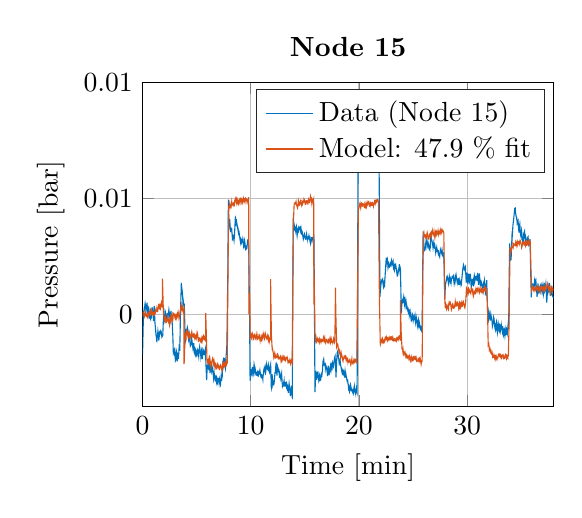
\begin{tikzpicture}

\begin{axis}[%
scaled y ticks = false,
 y tick label style={/pgf/number format/fixed,
/pgf/number format/1000 sep = \thinspace}, % Optional if you want to replace comma as the 1000 separator 
width=2.0556in,
height=1.62135in,
at={(1.011in,0.642in)},
scale only axis,
xmin=0,
xmax=38,
xlabel={Time [min]},
xmajorgrids,
ymin=-0.004,
ymax=0.01,
ylabel={Pressure [bar]},
ymajorgrids,
axis background/.style={fill=white},
title style={font=\bfseries},
title={Node 15},
legend style={legend cell align=left,align=left,draw=white!15!black}
]
\addplot [color=mycolor1,solid]
  table[row sep=crcr]{%
0.000833333333333333	-0.00173498670576727\\
0.0891666666666667	9.89526881719771e-05\\
0.12	9.63427174971443e-05\\
0.1675	0.000302530400781459\\
0.176666666666667	0.000249460997066825\\
0.2375	0.00045912864125125\\
0.264166666666667	0.000383439491691562\\
0.298333333333333	0.00023728113391952\\
0.363333333333333	0.000363429716518926\\
0.430833333333333	5.54531769304395e-05\\
0.439166666666667	7.98129032260064e-05\\
0.481666666666667	0.000341679960899829\\
0.526666666666667	0.00022945122189616\\
0.600833333333333	1.36936461380827e-05\\
0.614166666666667	0.000116352492668712\\
0.6975	-0.000153344477027584\\
0.7425	-0.0002125038123168\\
0.765833333333333	-6.98254154450212e-05\\
0.791666666666667	-0.000203803910068773\\
0.875833333333333	0.000263380840664962\\
0.915	0.000265990811339559\\
0.945833333333333	4.76232649068847e-05\\
0.965	0.000155502052785653\\
1.0075	-0.000298632844576471\\
1.0875	0.000352989833822023\\
1.13916666666667	-0.00031081270772243\\
1.22	-0.000771037536656027\\
1.22666666666667	-0.000757987683284611\\
1.315	-0.00117819296187882\\
1.32083333333333	-0.00118080293255253\\
1.4025	-0.000835416813296769\\
1.42166666666667	-0.000737977908116597\\
1.48916666666667	-0.00101811476050884\\
1.50416666666667	-0.00114165337243186\\
1.5725	-0.000771037536660302\\
1.57916666666667	-0.000775387487785287\\
1.605	-0.000863256500495166\\
1.675	-0.000738847898342235\\
1.75166666666667	-0.000866736461391682\\
1.75333333333333	-0.000862386510267751\\
1.7875	-0.000988535092868392\\
1.86916666666667	-0.000925025806452595\\
1.9275	-0.000222943695017713\\
1.96083333333333	-2.02359726333839e-05\\
2.00583333333333	-0.00032908250244823\\
2.015	-0.000256003323562126\\
2.08083333333333	0.000142452199407117\\
2.11333333333333	0.00010069266861841\\
2.16333333333333	-0.000312552688171042\\
2.1975	-0.000277753079179266\\
2.27666666666667	1.19536656829067e-05\\
2.32333333333333	2.3263538607321e-05\\
2.35916666666667	-0.000179444183775954\\
2.365	-8.20052785957814e-05\\
2.43583333333333	0.000187691691099806\\
2.45416666666667	0.000120702443786772\\
2.54	-0.000206413880742315\\
2.5625	-0.000250783382209352\\
2.6225	0.000141582209191429\\
2.62833333333333	0.000106782600197877\\
2.70583333333333	-0.000189014076251576\\
2.71583333333333	-0.000119414858265179\\
2.80333333333333	-0.000979835190616632\\
2.84583333333333	-0.00168887722385981\\
2.94416666666667	-0.00154706881720691\\
2.97583333333333	-0.00181241583577822\\
3.0025	-0.001641027761492\\
3.03416666666667	-0.00201425356794935\\
3.085	-0.00196292414468537\\
3.115	-0.00156272864125633\\
3.16833333333333	-0.00165581759531114\\
3.1975	-0.00204383323558623\\
3.275	-0.00166625747800672\\
3.31916666666667	-0.001937694428155\\
3.32833333333333	-0.00184547546432191\\
3.39666666666667	-0.00130521153470546\\
3.4425	-0.00158273841642503\\
3.50333333333333	-2.54559139829524e-05\\
3.585	0.00135173861192364\\
3.59083333333333	0.00127691945258911\\
3.67416666666667	0.000952413098726276\\
3.68	0.00098547272726926\\
3.75083333333333	0.00037038963831755\\
3.77666666666667	0.000518287976541743\\
3.8475	0.000252070967748\\
3.8575	0.000449558748783482\\
3.94166666666667	-0.00101811476051558\\
3.965	-0.00109902385142994\\
4.02416666666667	-0.000690128445760149\\
4.09916666666667	-0.000724058064521305\\
4.11666666666667	-0.000624879178885956\\
4.13916666666667	-0.000583119648093697\\
4.20416666666667	-0.000862386510264546\\
4.21583333333333	-0.000827586901271715\\
4.2525	-0.00107031417399561\\
4.32166666666667	-0.000870216422287129\\
4.37666666666667	-0.00122082248289423\\
4.37916666666667	-0.0011886328445751\\
4.41666666666667	-0.00137133079178575\\
4.48333333333333	-0.00131043147605148\\
4.53833333333333	-0.00104769442815672\\
4.55583333333333	-0.00109815386119755\\
4.64166666666667	-0.00142614017595583\\
4.65416666666667	-0.00146528973607508\\
4.68083333333333	-0.00127911182795976\\
4.73166666666667	-0.00127824183774017\\
4.80666666666667	-0.00168626725318397\\
4.8525	-0.00174629657869652\\
4.8825	-0.00151313919844077\\
4.9225	-0.00156185865103317\\
4.965	-0.00176195640274236\\
5.04916666666667	-0.00159665826002672\\
5.06666666666667	-0.0017175869012771\\
5.07916666666667	-0.00169496715543395\\
5.10666666666667	-0.00150356930596834\\
5.19333333333333	-0.00182198572825136\\
5.24583333333333	-0.00154619882698305\\
5.2775	-0.00141918025415926\\
5.34	-0.00161318807429857\\
5.34583333333333	-0.00157751847507974\\
5.39083333333333	-0.00184025552296524\\
5.45166666666667	-0.00161144809383522\\
5.51666666666667	-0.00193682443793897\\
5.5175	-0.0019281245356904\\
5.58416666666667	-0.00151313919841946\\
5.62916666666667	-0.00156359863146882\\
5.66666666666667	-0.00174629657869864\\
5.7275	-0.00175238651025289\\
5.75083333333333	-0.00164276774192551\\
5.80916666666667	-0.00151052922774646\\
5.8675	-0.00225872082111742\\
5.925	-0.00284683421309317\\
5.96083333333333	-0.00244228875854836\\
6.005	-0.00223349110458705\\
6.08583333333333	-0.00233006001955935\\
6.10833333333333	-0.00217781173021159\\
6.1625	-0.00213083225805626\\
6.2175	-0.00243097888563248\\
6.2375	-0.00254494760508343\\
6.305	-0.0022552408602035\\
6.35	-0.00223784105571916\\
6.39	-0.00242227898338959\\
6.39916666666667	-0.00248404828935768\\
6.47916666666667	-0.00234136989248518\\
6.4825	-0.0023309300097889\\
6.56833333333333	-0.0027850649071393\\
6.57083333333333	-0.00279463479961456\\
6.625	-0.00256147741935102\\
6.65583333333333	-0.00267196617790937\\
6.70833333333333	-0.00281290459433414\\
6.75916666666667	-0.0027259055718428\\
6.81666666666667	-0.00292165337243766\\
6.84333333333333	-0.0029686328445802\\
6.87166666666667	-0.00277549501466828\\
6.96166666666667	-0.00297646275660063\\
7.0025	-0.0027580952101669\\
7.0075	-0.0027807149560143\\
7.08333333333333	-0.00291556344085642\\
7.11333333333333	-0.00282508445747247\\
7.17666666666667	-0.00310696129034049\\
7.19083333333333	-0.00309478142719363\\
7.26583333333333	-0.00269458592377667\\
7.31166666666667	-0.00288250381232977\\
7.32833333333333	-0.00266065630499206\\
7.35666666666667	-0.00275548523950242\\
7.42833333333333	-0.00203774330399931\\
7.44666666666667	-0.00211430244377872\\
7.49333333333333	-0.00190289481915293\\
7.56666666666667	-0.0019194246334262\\
7.615	-0.00219869149560842\\
7.65333333333333	-0.00231527018574233\\
7.69916666666667	-0.00191942463342903\\
7.70583333333333	-0.00194378435972276\\
7.79	-0.00135915092862682\\
7.79333333333333	-0.00140352043009066\\
7.88166666666667	0.00173366432063382\\
7.93416666666667	0.00494392825023376\\
7.96916666666667	0.00416789696969069\\
8.05	0.00381294095795859\\
8.07916666666667	0.00391385982404167\\
8.13	0.00356934369501866\\
8.2075	0.00360240332356519\\
8.23166666666667	0.00373464183774425\\
8.31916666666667	0.00317871808406985\\
8.35333333333333	0.00341013548387714\\
8.42166666666667	0.00338925571848883\\
8.46166666666667	0.0032100377321644\\
8.49416666666667	0.00336489599218659\\
8.57583333333333	0.00415571710654526\\
8.59	0.00417137693058756\\
8.6575	0.00391472981425417\\
8.69416666666667	0.00397997908112196\\
8.755	0.003765961485826\\
8.75916666666667	0.00380511104594383\\
8.84416666666667	0.00357369364613086\\
8.8525	0.00362241309872112\\
8.91416666666667	0.00347103479960716\\
8.93166666666667	0.0035023544477074\\
9.01916666666667	0.00320046783967919\\
9.05083333333334	0.00311520879764836\\
9.075	0.00327006705766203\\
9.135	0.00322482756598\\
9.16333333333333	0.0030690993157439\\
9.24333333333333	0.00314217849461507\\
9.27166666666667	0.00325701720430126\\
9.28416666666667	0.00323178748778652\\
9.35416666666667	0.00288205141741181\\
9.38416666666667	0.00290902111437141\\
9.4325	0.00316218826979089\\
9.46833333333333	0.00306648934506662\\
9.52416666666667	0.00278374252199605\\
9.585	0.00281158220918379\\
9.61583333333333	0.00296818044965939\\
9.63666666666667	0.0028202821114352\\
9.71916666666667	0.00318567800586927\\
9.7325	0.00319785786901897\\
9.74083333333333	0.00306996930597059\\
9.80833333333333	0.00308997908113505\\
9.895	-0.000176834213112542\\
9.94083333333333	-0.00288337380254368\\
10.0291666666667	-0.00238051945260302\\
10.0683333333333	-0.00254929755622406\\
10.0908333333333	-0.00258235718476064\\
10.155	-0.00227612062560886\\
10.16	-0.00230135034213069\\
10.2258333333333	-0.00261106686216799\\
10.245	-0.00256756735092942\\
10.3083333333333	-0.00216824183774626\\
10.3358333333333	-0.00223436109483081\\
10.3883333333333	-0.00249883812317328\\
10.4233333333333	-0.00239530928641719\\
10.5066666666667	-0.0026284666666779\\
10.5658333333333	-0.00263977653961653\\
10.5883333333333	-0.00254233763443173\\
10.6125	-0.00250318807430538\\
10.6833333333333	-0.00266674623655055\\
10.6925	-0.00267109618767555\\
10.7225	-0.00250492805473036\\
10.7891666666667	-0.00255712746823739\\
10.8458333333333	-0.00242227898338249\\
10.8583333333333	-0.00246229853372135\\
10.9391666666667	-0.0027180756598323\\
11.0066666666667	-0.00274765532750045\\
11.0166666666667	-0.00262411671556712\\
11.0541666666667	-0.0026397765395938\\
11.1175	-0.00281203460409464\\
11.1208333333333	-0.00277549501465266\\
11.195	-0.00246751847504746\\
11.2083333333333	-0.00248752825022329\\
11.2566666666667	-0.00231440019548862\\
11.3408333333333	-0.00249361818182585\\
11.3733333333333	-0.00233788993159116\\
11.3975	-0.00244315874879923\\
11.4683333333333	-0.00221261133921295\\
11.475	-0.00216650185729854\\
11.5583333333333	-0.00238225943304932\\
11.6125	-0.00241705904207201\\
11.6416666666667	-0.00221348132946098\\
11.6491666666667	-0.00223349110463394\\
11.725	-0.00250927800590652\\
11.7408333333333	-0.00252667781038091\\
11.8216666666667	-0.00221870127078425\\
11.8408333333333	-0.00217346177908659\\
11.9025	-0.00316699061579406\\
11.9166666666667	-0.00319570029321418\\
11.97	-0.00259714701856062\\
11.9966666666667	-0.00271633567939594\\
12.0525	-0.00302605219941759\\
12.0916666666667	-0.00292513333333594\\
12.1466666666667	-0.0030025624633577\\
12.1716666666667	-0.00292948328444247\\
12.2483333333333	-0.00250666803517383\\
12.2616666666667	-0.00256930733136577\\
12.34	-0.00212822228741451\\
12.3525	-0.0021203923753898\\
12.4225	-0.00265456637344065\\
12.435	-0.00258844711634758\\
12.4858333333333	-0.00226133079177764\\
12.5508333333333	-0.00237268954059679\\
12.5741666666667	-0.00249100821115568\\
12.6091666666667	-0.00249013822094461\\
12.6791666666667	-0.00276592512216602\\
12.7025	-0.00257974721405496\\
12.7733333333333	-0.00278158494622679\\
12.855	-0.00256930733137999\\
12.8716666666667	-0.0027467853372439\\
12.8758333333333	-0.00273808543499676\\
12.9316666666667	-0.00311218123166092\\
13.015	-0.00298777262951083\\
13.03	-0.00312871104593276\\
13.0883333333333	-0.00289120371456413\\
13.1283333333333	-0.00310087135874645\\
13.145	-0.00309913137828452\\
13.2108333333333	-0.00295384301077312\\
13.245	-0.0029477530791933\\
13.2941666666667	-0.00316351065494977\\
13.335	-0.00321049012708094\\
13.3541666666667	-0.00303562209190424\\
13.4266666666667	-0.00314698084066939\\
13.4775	-0.00339753802542297\\
13.4858333333333	-0.00326529951124249\\
13.545	-0.00300430244380542\\
13.5725	-0.00312262111437284\\
13.6558333333333	-0.00349758690125376\\
13.6675	-0.00350280684259124\\
13.745	-0.00312001114367993\\
13.7683333333333	-0.00311566119258194\\
13.83	-0.00359850576733542\\
13.8391666666667	-0.00360546568913483\\
13.9225	0.00342231534699132\\
13.9333333333333	0.00405914819157155\\
14.025	0.00384252062560685\\
14.0808333333333	0.00359283343110413\\
14.1141666666667	0.00379119120236347\\
14.1358333333333	0.00360240332356804\\
14.2166666666667	0.00377292140760127\\
14.27	0.00344928504397793\\
14.2858333333333	0.00338925571847036\\
14.3483333333333	0.00365199276636936\\
14.3933333333333	0.00372159198431526\\
14.4316666666667	0.00358326353858907\\
14.465	0.00363285298145294\\
14.4958333333333	0.00374508172043769\\
14.5825	0.00377031143692541\\
14.6075	0.00362328308894355\\
14.6433333333333	0.00371724203324\\
14.7033333333333	0.00350757438905483\\
14.7391666666667	0.00355194389052436\\
14.7983333333333	0.00340578553273369\\
14.8041666666667	0.00341970537633821\\
14.86	0.00323526744866919\\
14.8941666666667	0.00329703675462732\\
14.9641666666667	0.00345276500485917\\
14.9733333333333	0.00343362521991147\\
15.0558333333333	0.0032439673509078\\
15.095	0.00323178748777089\\
15.1391666666667	0.00337794584553884\\
15.1616666666667	0.00345624496578019\\
15.2266666666667	0.00326484711634017\\
15.2366666666667	0.00335793607039997\\
15.2566666666667	0.00321264770283457\\
15.3233333333333	0.00325614721403902\\
15.3808333333333	0.00339621564024704\\
15.4116666666667	0.00333357634405794\\
15.4725	0.00316740821111133\\
15.4991666666667	0.00322917751708936\\
15.5433333333333	0.00304995953077487\\
15.5866666666667	0.00313782854349434\\
15.6416666666667	0.0033144365591415\\
15.7066666666667	0.00331356656890769\\
15.7508333333333	0.00314913841640029\\
15.7675	0.00311433880742876\\
15.8333333333333	0.00329268680349806\\
15.8491666666667	0.00317784809379199\\
15.9366666666667	-0.00334011867058272\\
15.94	-0.00336273841642587\\
16.015	-0.00244663870970604\\
16.0241666666667	-0.0024883982404912\\
16.0858333333333	-0.00280942463343585\\
16.1116666666667	-0.00280507468231796\\
16.1708333333333	-0.00250753802545879\\
16.2025	-0.00249796813298921\\
16.2858333333333	-0.00283465434997189\\
16.2866666666667	-0.00283204437929889\\
16.3658333333333	-0.0026284666666708\\
16.3783333333333	-0.00265717634406534\\
16.3991666666667	-0.00286684398825621\\
16.4616666666667	-0.00284944418378465\\
16.5425	-0.0025258078201329\\
16.5608333333333	-0.00271720566959849\\
16.6366666666667	-0.00237094956008937\\
16.6766666666667	-0.00204731319646605\\
16.7433333333333	-0.00194204437933755\\
16.7958333333333	-0.00218999159340391\\
16.8741666666667	-0.002147362072348\\
16.8983333333333	-0.00234919980451984\\
16.8991666666667	-0.00234658983384683\\
16.9508333333333	-0.00222305122191918\\
17	-0.00229439042033838\\
17.075	-0.00253798768328117\\
17.0891666666667	-0.00267457614858806\\
17.1616666666667	-0.00224480097755979\\
17.1625	-0.00224480097755979\\
17.245	-0.00263977653961653\\
17.25	-0.0026041069403913\\
17.3116666666667	-0.00237007956991242\\
17.3383333333333	-0.00241183910070042\\
17.4125	-0.00210125259043642\\
17.445	-0.00237616950148371\\
17.5108333333333	-0.0021882516129164\\
17.5358333333333	-0.00226046080156372\\
17.5625	-0.00210734252199919\\
17.6458333333333	-0.00224828093842966\\
17.6833333333333	-0.00207950283478446\\
17.6875	-0.00210560254152874\\
17.7508333333333	-0.00187331515150894\\
17.795	-0.00181589579670564\\
17.8625	-0.0024596885630796\\
17.8791666666667	-0.00272590557185132\\
17.95	-0.0019611841642483\\
18.0033333333333	-0.00163493782992069\\
18.0508333333333	-0.00158795835776679\\
18.1166666666667	-0.00193334447704209\\
18.1266666666667	-0.00187418514173991\\
18.18	-0.00212561231672445\\
18.2633333333333	-0.00197945395896504\\
18.2933333333333	-0.00221087135876238\\
18.3008333333333	-0.00217433176931471\\
18.3841666666667	-0.00238138944282404\\
18.3975	-0.00229787038123098\\
18.455	-0.00253537771262806\\
18.5133333333333	-0.00244924868036768\\
18.555	-0.00264238651027249\\
18.5741666666667	-0.00240922913001319\\
18.6466666666667	-0.00267283616812043\\
18.6741666666667	-0.00269545591396642\\
18.7241666666667	-0.00245272864124607\\
18.7383333333333	-0.00250144809385339\\
18.82	-0.00275983519060893\\
18.8283333333333	-0.00267544613879912\\
18.9125	-0.00289990361683116\\
18.9641666666667	-0.00286510400782553\\
18.9991666666667	-0.00302866217009629\\
19.0016666666667	-0.00299299257087675\\
19.0491666666667	-0.00323658983381953\\
19.1258333333333	-0.00313915092863049\\
19.1466666666667	-0.00333924868035744\\
19.1758333333333	-0.00330357908114358\\
19.2258333333333	-0.0030643317692931\\
19.2633333333333	-0.00314437086999354\\
19.3233333333333	-0.00329487917887085\\
19.3816666666667	-0.00326355953076352\\
19.4358333333333	-0.00339579804496104\\
19.4733333333333	-0.00343842756599422\\
19.5258333333333	-0.00322701994134994\\
19.5725	-0.00310783128056862\\
19.6125	-0.00335142854349718\\
19.6475	-0.00339318807428235\\
19.6625	-0.00321571006842696\\
19.7116666666667	-0.0034071079179096\\
19.76	-0.00320962013685282\\
19.8341666666667	-0.00336708836753523\\
19.8766666666667	0.00143003773216784\\
19.9325	0.00846303870966558\\
19.9916666666667	0.0079810641251033\\
20.0516666666667	0.00775573665688008\\
20.0775	0.00764611788856265\\
20.135	0.00790189501466508\\
20.1425	0.00794017458456331\\
20.2158333333333	0.00772441700876421\\
20.2708333333333	0.00770092727268157\\
20.3116666666667	0.00788971515145996\\
20.3575	0.00804805337239892\\
20.4016666666667	0.00779575620720899\\
20.4491666666667	0.00767569755616826\\
20.4958333333333	0.00768700742909126\\
20.5766666666667	0.00791929481913095\\
20.6008333333333	0.00798976402736465\\
20.6641666666667	0.00781054604106153\\
20.6716666666667	0.00782011593352544\\
20.735	0.00759739843596385\\
20.7558333333333	0.00770962717495145\\
20.7783333333333	0.00791407487780199\\
20.8591666666667	0.00765220782011689\\
20.9266666666667	0.00780532609969278\\
20.9308333333333	0.0077687865102508\\
20.9733333333333	0.00785056559138192\\
21.0433333333333	0.00771919706739831\\
21.0766666666667	0.00786187546426796\\
21.1266666666667	0.00786100547407678\\
21.1591666666667	0.00766525767348476\\
21.2041666666667	0.00766960762459981\\
21.25	0.00788188523947504\\
21.2775	0.00777313646138858\\
21.355	0.0081367923753323\\
21.365	0.00809416285432185\\
21.4408333333333	0.00779488621701213\\
21.4658333333333	0.00780358611925927\\
21.5233333333333	0.00795670439882379\\
21.5641666666667	0.00780010615833825\\
21.62	0.00798106412511751\\
21.6691666666667	0.00787318533722506\\
21.71	0.00800977380251773\\
21.7583333333333	0.00807154310849861\\
21.79	0.00784012570867852\\
21.8475	0.00799933391983423\\
21.89	0.00463247174974307\\
21.9408333333333	0.00074535542523968\\
21.9958333333333	0.00109161153471185\\
22.0591666666667	0.0013769683284398\\
22.0691666666667	0.0013569585532725\\
22.1166666666667	0.00145613743890359\\
22.1891666666667	0.00151442678395775\\
22.2341666666667	0.00128300938411208\\
22.2733333333333	0.00118383049854352\\
22.3283333333333	0.00135695855332935\\
22.3733333333333	0.00126560957966895\\
22.4158333333333	0.00161447565981412\\
22.5008333333333	0.00225913841647021\\
22.5308333333333	0.00219388914963653\\
22.5725	0.00240703675463756\\
22.6116666666667	0.00242791651996477\\
22.6783333333333	0.00208949032255142\\
22.6916666666667	0.00199379139783283\\
22.765	0.00212950987290875\\
22.7716666666667	0.00216604946234789\\
22.83	0.00205034076246485\\
22.8766666666667	0.00209906021502385\\
22.9133333333333	0.00217561935482601\\
22.9408333333333	0.00213385982408631\\
23.0116666666667	0.00232438768325843\\
23.0333333333333	0.0022747982404514\\
23.0633333333333	0.00213994975564624\\
23.155	0.00228523812316049\\
23.2	0.00195899178884425\\
23.2375	0.00192071221896023\\
23.2833333333333	0.00205904066474041\\
23.305	0.00195464183776331\\
23.355	0.00211993998047043\\
23.3925	0.00214777966767379\\
23.4658333333333	0.00192071221897727\\
23.5408333333333	0.00164492531769334\\
23.575	0.00164753528832939\\
23.6408333333333	0.00193028211139286\\
23.6525	0.00186938279566284\\
23.7291666666667	0.00208079042029291\\
23.735	0.0021529996089516\\
23.8091666666667	0.00179195366565815\\
23.8408333333333	0.00186851280543757\\
23.9041666666667	0.000428678983350403\\
23.9275	3.54434017442173e-05\\
23.97	0.000533947800615317\\
24.0291666666667	0.000603547018626582\\
24.0458333333333	0.000492188269830163\\
24.0808333333333	0.000503498142701994\\
24.1391666666667	0.000726215640300509\\
24.2108333333333	0.000439118866133376\\
24.2533333333333	0.000650526490774794\\
24.2558333333333	0.000656616422346101\\
24.3416666666667	0.000348639882686907\\
24.3708333333333	0.00048696832843298\\
24.41	0.000328630107584979\\
24.4291666666667	0.000362559726376693\\
24.5166666666667	0.000156372043035813\\
24.5533333333333	0.0001990015640633\\
24.5841666666667	-1.96617788610076e-06\\
24.6225	0.000210311436935132\\
24.6575	-6.28654936274814e-05\\
24.7341666666667	0.000110262561061711\\
24.7791666666667	-0.000106365004885936\\
24.7841666666667	-8.11352883641064e-05\\
24.8416666666667	-0.000289932942341045\\
24.8891666666667	-0.000246433431088267\\
24.9275	1.19536657354757e-05\\
24.9733333333333	-4.37257086428333e-05\\
25.0208333333333	-0.000282973020504673\\
25.1066666666667	-9.59251221825386e-05\\
25.1283333333333	-0.000204673900286056\\
25.1408333333333	-0.000145514564989568\\
25.2175	-0.00032125259040007\\
25.2308333333333	-0.000358662170092922\\
25.2733333333333	-6.63454546138698e-05\\
25.3133333333333	-0.000163784359731869\\
25.375	-0.000394331769323839\\
25.4058333333333	-0.000243823460423787\\
25.4516666666667	-0.0004865507331413\\
25.51	-0.000272533137852443\\
25.5566666666667	-0.00048133079181234\\
25.5883333333333	-0.000381281915961651\\
25.6508333333333	-0.000547450048865625\\
25.6816666666667	-0.000616179276606121\\
25.7158333333333	-0.000530050244325855\\
25.7425	-0.000543970087964488\\
25.7991666666667	-0.000717968132998334\\
25.8408333333333	-0.000671858651081075\\
25.9175	0.0029655704790077\\
25.9333333333333	0.00357021368523824\\
26.005	0.00289510127074842\\
26.0675	0.00274285298135234\\
26.0975	0.00275677282498528\\
26.18	0.00306213939391747\\
26.21	0.00296296050829206\\
26.25	0.00319263792769285\\
26.2775	0.00321525767349905\\
26.3558333333333	0.00295513059620199\\
26.4008333333333	0.00305430948185581\\
26.4433333333333	0.00292294095802\\
26.4575	0.00294991065498103\\
26.5008333333333	0.00282463206254598\\
26.5541666666667	0.00276982267833042\\
26.6083333333333	0.00307953919840608\\
26.6216666666667	0.00304821955031863\\
26.6441666666667	0.00332226647113494\\
26.7091666666667	0.003238747409576\\
26.7933333333333	0.0030804091886143\\
26.8525	0.00286030166172574\\
26.915	0.00307779921794982\\
26.9683333333333	0.00292468093833982\\
27.0066666666667	0.00298558025409826\\
27.0558333333333	0.00283507194523801\\
27.06	0.00286378162264961\\
27.0991666666667	0.00265324398819936\\
27.185	0.00286552160313427\\
27.215	0.00269152355812885\\
27.2333333333333	0.00279070244376563\\
27.3075	0.00265498396871813\\
27.3308333333333	0.00275938279566112\\
27.3633333333333	0.00257929481911284\\
27.4641666666667	0.00246358611926958\\
27.4933333333333	0.00266890381228856\\
27.5008333333333	0.00264280410554144\\
27.535	0.00279331241441874\\
27.59	0.00270892336265725\\
27.6533333333333	0.00261757438904234\\
27.6875	0.00276199276631993\\
27.7566666666667	0.00252448543499391\\
27.8008333333333	0.00247489599216984\\
27.8441666666667	0.00263410420329997\\
27.8483333333333	0.0026706437927448\\
27.9316666666667	0.000675756207165895\\
27.9358333333333	0.000655746431995757\\
28.01	0.00139871808410313\\
28.0216666666667	0.00132041896386177\\
28.1025	0.00153356656882871\\
28.11	0.00151877673501595\\
28.16	0.00163187546429705\\
28.1958333333333	0.00157445610947385\\
28.2666666666667	0.00134129872923446\\
28.2875	0.00143438768329425\\
28.3541666666667	0.00161447565978001\\
28.3691666666667	0.00154139648090741\\
28.4141666666667	0.00139001818178208\\
28.4633333333333	0.00151268680349013\\
28.5183333333333	0.0013569585532327\\
28.5441666666667	0.00147092727267656\\
28.6158333333333	0.00161099569890162\\
28.6541666666667	0.00158315601169257\\
28.7166666666667	0.00164927526880271\\
28.7191666666667	0.00162752551317631\\
28.7966666666667	0.00133955874873842\\
28.8066666666667	0.00138044828931534\\
28.8708333333333	0.00156227624629146\\
28.8983333333333	0.00142655777120987\\
28.9825	0.00169277478003274\\
29.07	0.00141350791788747\\
29.0941666666667	0.00135086862168983\\
29.1533333333333	0.00151616676436284\\
29.1883333333333	0.00152399667641881\\
29.2233333333333	0.00128909931568338\\
29.2716666666667	0.00129170928633648\\
29.3108333333333	0.00144830752687604\\
29.345	0.00134390869990463\\
29.3591666666667	0.00142655777124966\\
29.4608333333333	0.00128996930590866\\
29.5075	0.00150311691100065\\
29.595	0.00192071221901138\\
29.6641666666667	0.00212776989246387\\
29.6858333333333	0.00209384027371194\\
29.7441666666667	0.00192158220914572\\
29.8366666666667	0.00203555092864641\\
29.8575	0.00189896246335089\\
29.92	0.0013613085043705\\
29.945	0.00150311691104044\\
30	0.00179108367546697\\
30.07	0.00128474936460243\\
30.1191666666667	0.00164318533728824\\
30.1308333333333	0.0017510641251608\\
30.1983333333333	0.00144134760508514\\
30.2141666666667	0.00141263792768492\\
30.2633333333333	0.00171626451613811\\
30.3025	0.0017188744867685\\
30.3833333333333	0.00111684125119105\\
30.4675	0.00150137693061261\\
30.4816666666667	0.00149963695014499\\
30.525	0.00127430948195589\\
30.5758333333333	0.00124559980452724\\
30.61	0.0015335665689083\\
30.6616666666667	0.00165014525905072\\
30.6916666666667	0.00138044828934945\\
30.7525	0.00148658709677144\\
30.775	0.00161447565982549\\
30.8383333333333	0.00163013548381237\\
30.9075	0.00146831730197797\\
30.9158333333333	0.00143438768322604\\
30.9741666666667	0.00178412375365333\\
30.9958333333333	0.00158663597262781\\
31.0583333333333	0.00126125962849706\\
31.1358333333333	0.00175802404686075\\
31.1658333333333	0.001548356402704\\
31.1741666666667	0.00158576598240821\\
31.2241666666667	0.00122037008799972\\
31.2816666666667	0.00123254995111957\\
31.3166666666667	0.00138305826003099\\
31.35	0.0013360787878714\\
31.4258333333333	0.00109161153470333\\
31.4333333333333	0.00115077086998845\\
31.5066666666667	0.00130214916907399\\
31.5216666666667	0.00122472003908634\\
31.6075	0.00145526744866693\\
31.6091666666667	0.00144395757574962\\
31.6691666666667	0.00119514037143241\\
31.7	0.0011994903225645\\
31.7325	0.000796684848497264\\
31.8133333333333	0.00147092727269929\\
31.8716666666667	0.000455648680334167\\
31.9366666666667	-0.000374321994085491\\
31.9991666666667	-8.37452590172205e-05\\
32.0208333333333	9.89526881784997e-05\\
32.0825	-3.67657869087823e-05\\
32.1066666666667	-0.000251653372457028\\
32.1366666666667	-0.000256003323532275\\
32.1908333333333	5.86373419260433e-06\\
32.2216666666667	-7.59153469612472e-05\\
32.3091666666667	-0.000334302443762258\\
32.3366666666667	-0.000532660215035813\\
32.3983333333333	-0.00041521153466241\\
32.4475	-0.000127244770213142\\
32.4858333333333	-0.000182924144619886\\
32.5708333333333	-0.000604869403779768\\
32.6225	-0.000687518475113433\\
32.6591666666667	-0.000438701270762107\\
32.7083333333333	-0.000338652394888672\\
32.745	-0.000569199804520429\\
32.7616666666667	-0.00052309032260317\\
32.8066666666667	-0.000807577126145625\\
32.8433333333333	-0.000710138220913939\\
32.8841666666667	-0.000429131378261255\\
32.9625	-0.000657938807396966\\
32.9975	-0.000454361094783085\\
33.0375	-0.000483070772268585\\
33.0758333333333	-0.000726668035222741\\
33.1083333333333	-0.000640539002919729\\
33.1575	-0.000446531182755547\\
33.2383333333333	-0.000694478396847484\\
33.2583333333333	-0.000537010166173593\\
33.2941666666667	-0.000545710068454844\\
33.3258333333333	-0.000745807820161912\\
33.3608333333333	-0.00061965923752999\\
33.3841666666667	-0.000885876246369932\\
33.4616666666667	-0.000711008211230171\\
33.5016666666667	-0.000923285826108247\\
33.5675	-0.000674468621700078\\
33.6133333333333	-0.000899796089946031\\
33.6241666666667	-0.000824976930617172\\
33.6575	-0.000696218377298052\\
33.7141666666667	-0.000836286803500383\\
33.7975	-0.000418691495614701\\
33.8425	-0.000520480351881847\\
33.885	0.00153704652987195\\
33.9308333333333	0.00305256950151325\\
33.9991666666667	0.00243313646136763\\
34.0308333333333	0.00233830752686295\\
34.0641666666667	0.00234961739975753\\
34.1475	0.00335619608988687\\
34.165	0.00330921661773864\\
34.2358333333333	0.00382947077223612\\
34.3233333333333	0.00418790674487078\\
34.4	0.00456374252201677\\
34.4508333333333	0.00457766236561562\\
34.4925	0.00429839550345329\\
34.4983333333333	0.00432014525909104\\
34.5816666666667	0.00410612766367145\\
34.5908333333333	0.00417398690123215\\
34.63	0.00391385982404309\\
34.71	0.00402434858270517\\
34.7583333333333	0.00370593216036533\\
34.7908333333333	0.00351540430106817\\
34.8483333333333	0.00382686080153755\\
34.8725	0.00389124007818574\\
34.9358333333333	0.00343188523944669\\
34.9808333333333	0.0033396662755667\\
35.0233333333333	0.00356064379274308\\
35.0333333333333	0.0036006633431061\\
35.1108333333333	0.00326049716512281\\
35.1516666666667	0.00307605923745946\\
35.1983333333333	0.00326571710649724\\
35.2033333333333	0.00325005728245352\\
35.2425	0.0034945245356159\\
35.3125	0.00358413352882572\\
35.3425	0.00332574643205881\\
35.375	0.00336054604107013\\
35.3975	0.00307344926685182\\
35.4616666666667	0.00312999863144975\\
35.5266666666667	0.00325701720423872\\
35.5625	0.00315522834796021\\
35.6358333333333	0.00332052649066164\\
35.6383333333333	0.00332313646134318\\
35.6958333333333	0.00298732023457725\\
35.7258333333333	0.0030177698924394\\
35.8116666666667	0.00321177771259223\\
35.8191666666667	0.00323526744865782\\
35.8991666666667	0.00133607878787707\\
35.9341666666667	0.000724475659815843\\
35.9958333333333	0.00134912864120516\\
36.0108333333333	0.00117252062558074\\
36.1266666666667	0.0012656095796519\\
36.155	0.00112380117300469\\
36.1658333333333	0.00114468093840579\\
36.235	0.0014413476050283\\
36.2741666666667	0.00130736911040863\\
36.3358333333333	0.00146918729225441\\
36.35	0.00148484711626971\\
36.4183333333333	0.00104289208209885\\
36.4241666666667	0.00104724203320822\\
36.4658333333333	0.000747965395875738\\
36.5116666666667	0.000966332942262588\\
36.5458333333333	0.00132563890510547\\
36.62	0.00100548250243443\\
36.6525	0.00109596148575584\\
36.7166666666667	0.000977642815270852\\
36.7741666666667	0.00120732023455794\\
36.78	0.00122124007816247\\
36.8358333333333	0.00108639159330615\\
36.8841666666667	0.00121167018572983\\
36.925	0.000999392570851756\\
36.9925	0.00120645024438382\\
37.0291666666667	0.000885423851459066\\
37.045	0.00084366432065118\\
37.125	0.00130127917887145\\
37.1308333333333	0.00135260860212903\\
37.1691666666667	0.00100635249259717\\
37.2233333333333	0.00110901133915214\\
37.28	0.00131345904192309\\
37.3008333333333	0.00118557047889177\\
37.3533333333333	0.000497408211125011\\
37.3875	0.000666186314795786\\
37.455	0.00125429970671753\\
37.475	0.00117861055713497\\
37.5191666666667	0.00103245219935566\\
37.6016666666667	0.0013491286412279\\
37.6383333333333	0.00111684125121379\\
37.6525	0.00115251085043333\\
37.7108333333333	0.000815824633425069\\
37.7491666666667	0.000828874486798636\\
37.7941666666667	0.00101157243403414\\
37.8366666666667	0.00105420195506163\\
37.8791666666667	0.000797554838694134\\
38	0.000690546041063916\\
};
\addlegendentry{Data (Node 15)};

\addplot [color=mycolor2,solid]
  table[row sep=crcr]{%
0.000833333333333333	6.06187453698676e-06\\
0.00166666666666667	-0.000115813800586548\\
0.0183333333333333	8.45029472803595e-05\\
0.118333333333333	3.84064742025831e-05\\
0.175	-6.46725328109068e-05\\
0.178333333333333	-8.43275929506392e-05\\
0.264166666666667	6.02138159321746e-05\\
0.309166666666667	-7.31159440057355e-05\\
0.410833333333333	-0.000119958530645137\\
0.428333333333333	-2.83771457710013e-05\\
0.465	-0.00010128724739106\\
0.523333333333333	-1.58789953862991e-05\\
0.533333333333333	-8.76243189798742e-05\\
0.596666666666667	3.8805485380692e-05\\
0.634166666666667	-5.08406045222511e-06\\
0.700833333333333	0.000117419342026579\\
0.701666666666667	0.000110018764059274\\
0.766666666666667	-3.80136663656733e-07\\
0.803333333333333	0.000146206052240378\\
0.875833333333333	3.50622484809282e-05\\
0.908333333333333	8.11911150743559e-05\\
0.945	-3.49543821929154e-05\\
0.995833333333333	-4.45911495459406e-05\\
1.01916666666667	7.25660605090318e-05\\
1.05916666666667	8.33903374627546e-05\\
1.09833333333333	-2.45240879832667e-05\\
1.14666666666667	3.05072656178409e-05\\
1.215	0.000166257924113557\\
1.23333333333333	0.000110148512862691\\
1.315	0.000212931356710665\\
1.32166666666667	0.000237661107658065\\
1.36666666666667	0.000110814223940637\\
1.4025	0.000112746912661242\\
1.48583333333333	0.000423511157601416\\
1.51333333333333	0.000429857832686913\\
1.54833333333333	0.000260335539035888\\
1.6025	0.000218694669515602\\
1.635	0.000342193308609858\\
1.66666666666667	0.000277158578841013\\
1.75	0.000486686506538751\\
1.8325	0.000286067822049011\\
1.83583333333333	0.0015330257469771\\
1.845	0.00145154307182694\\
1.9275	8.2000363938623e-05\\
2.0125	-0.000248629559245841\\
2.02166666666667	-0.000288182391890481\\
2.1025	-0.000145781256192761\\
2.1775	-0.000358965889737777\\
2.19833333333333	-0.000361281932480433\\
2.2725	-0.000195093918049143\\
2.28833333333333	-0.000232964546879384\\
2.3325	-0.000121469155627483\\
2.36666666666667	-0.00019801581358815\\
2.405	-0.000326657882769582\\
2.46166666666667	-0.00024566390532483\\
2.50583333333333	-0.000470347757792865\\
2.545	-0.000387175605146\\
2.61583333333333	-0.000121347667785771\\
2.65916666666667	-0.000226061664127239\\
2.6875	-8.85767499444604e-05\\
2.76666666666667	-0.000214274710393731\\
2.7925	-6.3259346489891e-05\\
2.82166666666667	-0.000139056965083498\\
2.85083333333333	3.14961054407488e-05\\
2.905	7.56707940827595e-06\\
2.96916666666667	-0.000102567233126987\\
2.99666666666667	1.55648306042347e-05\\
3.03416666666667	-0.00019340566807306\\
3.08083333333333	-0.000235980669353191\\
3.12916666666667	-4.55794795501631e-05\\
3.19083333333333	1.4639673566127e-05\\
3.21	-0.000110761736232541\\
3.24166666666667	-6.40928727550273e-05\\
3.29333333333333	7.83667808992709e-05\\
3.32916666666667	-2.24790480251359e-05\\
3.37666666666667	-0.000199330752462528\\
3.41916666666667	-9.37146306963039e-05\\
3.50333333333333	0.000200378335723579\\
3.505	0.000165641738629787\\
3.5625	0.00036669963130512\\
3.63666666666667	0.00017638647421829\\
3.67833333333333	0.000288399898788887\\
3.68	0.000316474886466937\\
3.76333333333333	0.00011562942010142\\
3.83416666666667	0.000220383276875269\\
3.83583333333333	-0.00216045700589476\\
3.855	-0.00205108207704272\\
3.94	-0.000823289633775264\\
3.9525	-0.000825371275110592\\
4.0225	-0.000998206557248122\\
4.03	-0.000924684995642697\\
4.07083333333333	-0.00073051968743153\\
4.1675	-0.000896458397092806\\
4.18416666666667	-0.000770162681960047\\
4.21083333333333	-0.000789427662697155\\
4.2675	-0.000990353483804323\\
4.32083333333333	-0.000859046314547703\\
4.375	-0.000974260088201799\\
4.39416666666667	-0.000898471771613851\\
4.4625	-0.000998515093760783\\
4.46833333333333	-0.000976840063552351\\
4.55166666666667	-0.000764999188771978\\
4.5575	-0.000778997039802997\\
4.63	-0.000977798271968039\\
4.66166666666667	-0.000989653558104598\\
4.705	-0.000899310349323656\\
4.76916666666667	-0.000981038827210239\\
4.78166666666667	-0.000864568229601953\\
4.84833333333333	-0.000904438186799417\\
4.865	-0.00107153968627842\\
4.90583333333333	-0.00103783502609642\\
4.97916666666667	-0.000913024108260045\\
4.99833333333333	-0.000981008583791099\\
5.0475	-0.000781647685342857\\
5.08083333333333	-0.000831603935660667\\
5.16666666666667	-0.0011801083398536\\
5.17666666666667	-0.00118016384554316\\
5.19666666666667	-0.00103163216857279\\
5.27	-0.00102640549447087\\
5.31083333333333	-0.00113939653610543\\
5.36833333333333	-0.00118601867698611\\
5.41083333333333	-0.00107840615676401\\
5.43333333333333	-0.00118019403353641\\
5.50166666666667	-0.00106088044437377\\
5.5225	-0.00114814440506678\\
5.59916666666667	-0.000999642434452582\\
5.62416666666667	-0.00102691701418471\\
5.64166666666667	-0.000918063801241701\\
5.6975	-0.000945933645040101\\
5.75833333333333	-0.00111719248901365\\
5.8325	-0.00115981752321288\\
5.83583333333333	4.58967374707648e-05\\
5.8675	-0.000366622230886384\\
5.955	-0.0019668664657352\\
5.95916666666667	-0.00192376520890929\\
5.9925	-0.00208558848585333\\
6.075	-0.00198276292662323\\
6.10666666666667	-0.00209074787925211\\
6.15666666666667	-0.00193455651405967\\
6.185	-0.00204312343838112\\
6.22416666666667	-0.00192523572219881\\
6.305	-0.00220003304261741\\
6.31666666666667	-0.00226427195513484\\
6.3925	-0.0020528065303221\\
6.39333333333333	-0.00207218749454782\\
6.47166666666667	-0.00192018532578917\\
6.48166666666667	-0.00194085363217489\\
6.565	-0.00214763742160003\\
6.60333333333333	-0.0020122841294061\\
6.6525	-0.00217744997051494\\
6.6825	-0.0022763484137575\\
6.72666666666667	-0.00212767469889443\\
6.74666666666667	-0.00214247534184019\\
6.80916666666667	-0.00235492394055063\\
6.85166666666667	-0.00231067848635781\\
6.91833333333333	-0.00215617898551618\\
6.935	-0.00214158402835405\\
6.97666666666667	-0.0022692508056368\\
7.00916666666667	-0.00222857448993431\\
7.08583333333333	-0.00238380903303208\\
7.095	-0.00238720261885211\\
7.17083333333333	-0.00221126620291423\\
7.20333333333333	-0.00219039942704128\\
7.2675	-0.00231593729179898\\
7.3175	-0.00239806270236783\\
7.355	-0.00229631793132052\\
7.36833333333333	-0.00234541907153427\\
7.4275	-0.00210087176599062\\
7.45	-0.00214365204944866\\
7.47666666666667	-0.00228217470600841\\
7.56833333333333	-0.00212906779697427\\
7.61583333333333	-0.00226106505240253\\
7.63666666666667	-0.00223724519512085\\
7.69166666666667	-0.00209445295945884\\
7.74416666666667	-0.00218218607503997\\
7.79333333333333	-0.00199894625800921\\
7.83333333333333	-0.00204450523575023\\
7.88166666666667	0.000963876219730098\\
7.9575	0.00451686762310513\\
7.9775	0.00448796581588279\\
8.05416666666667	0.00476151228342247\\
8.0625	0.00478923046508125\\
8.13583333333333	0.00458656662456678\\
8.16916666666667	0.00457885160797644\\
8.22083333333333	0.00474396821466025\\
8.24583333333333	0.00485308019585328\\
8.285	0.00472287535601178\\
8.36833333333333	0.00477638668157762\\
8.39583333333333	0.00467066865671976\\
8.40666666666667	0.00467176754795783\\
8.48083333333333	0.00482224499137775\\
8.5	0.00476189053250515\\
8.58166666666667	0.00496978760823723\\
8.61333333333334	0.00500866539002951\\
8.66916666666667	0.00484490256752059\\
8.68416666666667	0.00493653126900397\\
8.7475	0.00483757946085178\\
8.75833333333333	0.00493782520539215\\
8.8425	0.00479556158804509\\
8.84416666666667	0.00480701894549226\\
8.91333333333333	0.00491573376813303\\
8.93416666666667	0.00482483337627059\\
9.01916666666667	0.00493407061738345\\
9.03166666666667	0.00485150255850728\\
9.09	0.00499805896749941\\
9.1175	0.00499991641559617\\
9.17166666666667	0.00483179068355375\\
9.21	0.00491134132127821\\
9.25916666666667	0.00480819830515198\\
9.2825	0.0048546175834119\\
9.32416666666667	0.0050068171581356\\
9.4075	0.00487355821229874\\
9.44166666666667	0.00498834768051718\\
9.50333333333333	0.00501032244657231\\
9.545	0.00488072984481806\\
9.56166666666667	0.0048377806400692\\
9.61833333333333	0.00496971564491689\\
9.63333333333333	0.0049703178664903\\
9.71916666666667	0.00486028026667951\\
9.72583333333333	0.00484263733243589\\
9.80416666666667	0.00501745574948175\\
9.81	0.00505124095972339\\
9.83583333333333	-4.68755493633058e-06\\
9.895	0.000904470022099563\\
9.955	-0.000971747482199954\\
10.0141666666667	-0.000887404355796104\\
10.0616666666667	-0.00101397910178276\\
10.0833333333333	-0.000965550104362023\\
10.1458333333333	-0.000824228163219189\\
10.1808333333333	-0.000873651024218674\\
10.2291666666667	-0.00110322751637298\\
10.2858333333333	-0.00108099483396214\\
10.3233333333333	-0.000909448288358086\\
10.3683333333333	-0.000871712420844335\\
10.4191666666667	-0.000972347175634343\\
10.4225	-0.000949201479723617\\
10.4891666666667	-0.00105547319349825\\
10.5583333333333	-0.00086834516388339\\
10.5916666666667	-0.00101032977916544\\
10.6008333333333	-0.000949679606416316\\
10.6416666666667	-0.00108317860796951\\
10.6841666666667	-0.00106764761497508\\
10.77	-0.000905470945287827\\
10.7725	-0.000908299693547463\\
10.8541666666667	-0.00111864492748588\\
10.87	-0.00101046227075646\\
10.9233333333333	-0.00112792310876382\\
10.95	-0.00114290286143839\\
11.0275	-0.00091863701360669\\
11.035	-0.000910141681732157\\
11.0583333333333	-0.00108151345893342\\
11.1766666666667	-0.000878232826665584\\
11.2	-0.00100752811723566\\
11.2183333333333	-0.000917001080562214\\
11.2591666666667	-0.00108733852550646\\
11.2975	-0.00104007342354077\\
11.355	-0.000851004647322701\\
11.3833333333333	-0.000908669690159294\\
11.4666666666667	-0.00104198328814256\\
11.4816666666667	-0.00106179388536523\\
11.5583333333333	-0.000934655022081242\\
11.5975	-0.00104462089347757\\
11.61	-0.00092345219131992\\
11.6508333333333	-0.000972209383333864\\
11.7175	-0.0011846719418054\\
11.7358333333333	-0.0011427086735976\\
11.8183333333333	-0.000987532434216189\\
11.8341666666667	-0.00101540913612579\\
11.8358333333333	0.00151314973298291\\
11.9091666666667	-0.000899460982893714\\
11.9866666666667	-0.00155297988362344\\
12.0025	-0.00148335599954828\\
12.0841666666667	-0.0016742226450441\\
12.1366666666667	-0.00188116812124039\\
12.1775	-0.00181393958051341\\
12.2266666666667	-0.00168112570415184\\
12.26	-0.00174657296860557\\
12.2825	-0.00189644666623598\\
12.3891666666667	-0.00186015548159076\\
12.4341666666667	-0.00174995464606457\\
12.46	-0.00172722909108476\\
12.5133333333333	-0.00185603908647421\\
12.5416666666667	-0.0018082240237217\\
12.6083333333333	-0.00194728066809796\\
12.61	-0.00194782192808758\\
12.6941666666667	-0.00185275527596782\\
12.7408333333333	-0.00181844616692239\\
12.7825	-0.00196863523711408\\
12.8	-0.00202903547120671\\
12.86	-0.00190032602668133\\
12.885	-0.00186072693191849\\
12.9116666666667	-0.0019876178103077\\
13.0025	-0.00184605761397269\\
13.0458333333333	-0.00197003435237177\\
13.0725	-0.00197721843113957\\
13.1225	-0.00188591105146879\\
13.135	-0.00192397394428706\\
13.1991666666667	-0.00201231770437945\\
13.2316666666667	-0.00197536026728957\\
13.2675	-0.00185454888476296\\
13.33	-0.00186371830832935\\
13.3975	-0.0019716646023631\\
13.4016666666667	-0.0019518868094368\\
13.4558333333333	-0.00210741508570048\\
13.485	-0.0020934995146302\\
13.495	-0.00201666565810133\\
13.5733333333333	-0.00206976200293708\\
13.6225	-0.00195681873628172\\
13.66	-0.00202092304578201\\
13.6916666666667	-0.0021357399119041\\
13.7775	-0.00197966532106502\\
13.8333333333333	-0.00209631010439694\\
13.835	-0.0020666129597565\\
13.9225	0.0036905494787517\\
14.0091666666667	0.00472737365534573\\
14.0116666666667	0.00470661506972273\\
14.0358333333333	0.0047851297795395\\
14.0983333333333	0.00475449613436629\\
14.1825	0.00485859997782302\\
14.185	0.00482891596970025\\
14.2716666666667	0.00465600635140684\\
14.325	0.00458590436071462\\
14.3591666666667	0.00470315467382416\\
14.3625	0.00467293371161931\\
14.4058333333333	0.00490924264066185\\
14.4516666666667	0.00482990944134479\\
14.4866666666667	0.0047003344598066\\
14.5375	0.00472988574046773\\
14.6208333333333	0.00492372429767713\\
14.6391666666667	0.00492166153814695\\
14.7041666666667	0.00469611177521276\\
14.715	0.00468013575616377\\
14.7816666666667	0.00481711002097089\\
14.8	0.00476561728820698\\
14.8833333333333	0.00487765266028124\\
14.8875	0.00481400266194477\\
14.9233333333333	0.00497185785410331\\
14.9841666666667	0.00490804729466721\\
15.0491666666667	0.00473073124557657\\
15.0825	0.00473698845367143\\
15.1291666666667	0.0048893517173693\\
15.18	0.00489950425787061\\
15.2283333333333	0.00479204288838196\\
15.2775	0.0047605259648199\\
15.3216666666667	0.00490191422199049\\
15.3383333333333	0.00494381872143915\\
15.405	0.00482573800533527\\
15.4158333333333	0.00482171869704843\\
15.4966666666667	0.00500110037315306\\
15.5166666666667	0.0050773366755786\\
15.585	0.00492467684854266\\
15.5991666666667	0.00483017720826192\\
15.645	0.00499336072522415\\
15.68	0.0049689318958264\\
15.7391666666667	0.00480560695508105\\
15.8191666666667	0.00495858759287449\\
15.8358333333333	0.00040479485653819\\
15.8491666666667	0.00215855196930669\\
15.9366666666667	-0.000861094430717441\\
15.995	-0.00112010612693899\\
16.0375	-0.00100612266129026\\
16.0983333333333	-0.00120095410704272\\
16.1325	-0.00116370269380975\\
16.1875	-0.00106181513363039\\
16.2241666666667	-0.0011299254451902\\
16.2316666666667	-0.0010714888214353\\
16.3125	-0.0010764677581244\\
16.3566666666667	-0.00118060890994714\\
16.3808333333333	-0.00106043321299252\\
16.445	-0.00113360735570707\\
16.485	-0.00120333979757199\\
16.5258333333333	-0.00108352860664093\\
16.56	-0.00108402762465869\\
16.6058333333333	-0.00118146838250348\\
16.65	-0.00116384926235989\\
16.7158333333333	-0.00105578789066853\\
16.7325	-0.00101344343627045\\
16.7833333333333	-0.0011577935670783\\
16.8416666666667	-0.00102760499524508\\
16.8791666666667	-0.00118158373701807\\
16.925	-0.00124354490848927\\
16.985	-0.00109511241412109\\
17.0208333333333	-0.0010857802802654\\
17.0741666666667	-0.00119116354711204\\
17.135	-0.0012367325514105\\
17.1575	-0.00115022673993619\\
17.1841666666667	-0.0011156227181369\\
17.2366666666667	-0.00119718137004361\\
17.3175	-0.00105397911234044\\
17.335	-0.00116624223493778\\
17.3725	-0.00123623125853436\\
17.425	-0.0010865280835262\\
17.4375	-0.00105744600375184\\
17.5108333333333	-0.00121567703356674\\
17.5791666666667	-0.00124864394976383\\
17.595	-0.00116839727571688\\
17.6	-0.00120048010531349\\
17.66	-0.00106275085954873\\
17.6875	-0.00112551475796065\\
17.7425	-0.0012366240878345\\
17.775	-0.00119846308368978\\
17.8358333333333	0.00114551447488843\\
17.8625	8.84654642315835e-05\\
17.945	-0.00140533586206652\\
17.9533333333333	-0.00139270327150511\\
17.985	-0.00126906381721593\\
18.04	-0.00128936653708514\\
18.1225	-0.0015827451151029\\
18.125	-0.00155248945119162\\
18.21	-0.0016794237448453\\
18.2175	-0.00163399062083787\\
18.2966666666667	-0.00184052339938811\\
18.3	-0.00181432338104046\\
18.35	-0.0016560264309841\\
18.3883333333333	-0.00176016070452101\\
18.4758333333333	-0.00193399567993015\\
18.48	-0.00190234979227865\\
18.5333333333333	-0.00201510767098822\\
18.5641666666667	-0.0019298491698039\\
18.6233333333333	-0.00183925085630137\\
18.6566666666667	-0.00188359269697102\\
18.725	-0.00181068126217344\\
18.75	-0.00184588166449797\\
18.8066666666667	-0.00196591378571239\\
18.8291666666667	-0.00188071700504824\\
18.9133333333333	-0.00200054178192555\\
18.9558333333333	-0.00194427524261956\\
18.9808333333333	-0.00205269157269616\\
19.0041666666667	-0.00198258885226249\\
19.08	-0.00206055307454011\\
19.0958333333333	-0.00203421929680318\\
19.1641666666667	-0.00195812443431315\\
19.1775	-0.0019749904906641\\
19.2533333333333	-0.00218668140784697\\
19.2666666666667	-0.00216739287157557\\
19.3466666666667	-0.00193842230887415\\
19.3541666666667	-0.00198047011219992\\
19.4291666666667	-0.00214419665237314\\
19.4508333333333	-0.00215015324286057\\
19.5241666666667	-0.0019834689813689\\
19.5408333333333	-0.00195697215636567\\
19.6083333333333	-0.00208876125807451\\
19.6291666666667	-0.00207556027912124\\
19.68	-0.00194354338490682\\
19.7075	-0.00194346186745703\\
19.7841666666667	-0.00208362772127708\\
19.8033333333333	-0.0020986005653806\\
19.8766666666667	0.000837212559763999\\
19.9491666666667	0.00459216629944795\\
19.9716666666667	0.00453724987453132\\
20.0416666666667	0.00471267201823659\\
20.0975	0.00479078053613585\\
20.1383333333333	0.00464052587946256\\
20.1691666666667	0.004573087120524\\
20.215	0.00476212908763108\\
20.2408333333333	0.00478375493986137\\
20.2925	0.00466637458034736\\
20.3191666666667	0.00466293031026927\\
20.3575	0.0047680876616718\\
20.4458333333333	0.00474247874383276\\
20.4708333333333	0.00463189918978515\\
20.5183333333333	0.0046106143761224\\
20.5483333333333	0.00475222420433978\\
20.6258333333333	0.00463324759804434\\
20.6591666666667	0.00475541451101566\\
20.7	0.00463757030014182\\
20.7475	0.00474412522405063\\
20.7541666666667	0.00466341512297992\\
20.7966666666667	0.00479653020968949\\
20.86	0.00483482206803221\\
20.9158333333333	0.00475415678895177\\
20.9333333333333	0.00480149225170897\\
21.0033333333333	0.00465430660874824\\
21.0341666666667	0.00464218150528796\\
21.0783333333333	0.00482550810042506\\
21.1316666666667	0.00481208653516616\\
21.165	0.0046970266220667\\
21.2291666666667	0.00469517075297837\\
21.2708333333333	0.00480011476830128\\
21.3125	0.00477718478128674\\
21.3483333333333	0.00466391298605211\\
21.3733333333333	0.00472051604824109\\
21.4383333333333	0.00486222881582634\\
21.4841666666667	0.00478689748605242\\
21.5025	0.00490111126668065\\
21.5583333333333	0.00491997308465106\\
21.5858333333333	0.00480531524892291\\
21.6416666666667	0.00484428216279842\\
21.7133333333333	0.00495872518159358\\
21.745	0.00496063446274374\\
21.7983333333333	0.00483890728329314\\
21.81	0.00488792546142298\\
21.89	0.00077174731654592\\
21.9741666666667	-0.0012579543609343\\
21.985	-0.00129942348277229\\
22.0608333333333	-0.00113981812226976\\
22.1283333333333	-0.0010678483846379\\
22.1508333333333	-0.00116751281892805\\
22.18	-0.00110299588607176\\
22.2125	-0.00121906753846511\\
22.2525	-0.00123833003837207\\
22.3116666666667	-0.00113859899971791\\
22.3483333333333	-0.00118722650521537\\
22.4158333333333	-0.00102888630415429\\
22.4825	-0.000986708493761763\\
22.5033333333333	-0.00106997866003881\\
22.5316666666667	-0.00102112438035744\\
22.5433333333333	-0.00109420098881998\\
22.63	-0.00103654372823706\\
22.6591666666667	-0.0011360496567646\\
22.6891666666667	-0.0010966091020575\\
22.7616666666667	-0.00102190237596817\\
22.7816666666667	-0.00100264296145034\\
22.8016666666667	-0.00110084997802424\\
22.885	-0.00101333379902356\\
22.9266666666667	-0.00110781852539142\\
22.9658333333333	-0.00110533556015884\\
23.0108333333333	-0.000988724783102711\\
23.0441666666667	-0.00100550541991078\\
23.0891666666667	-0.0010870521664792\\
23.1341666666667	-0.00100268764668622\\
23.2	-0.00115046645099496\\
23.2066666666667	-0.00115345084280805\\
23.29	-0.00106723698535438\\
23.3116666666667	-0.001073091802967\\
23.3316666666667	-0.00115190201499594\\
23.3958333333333	-0.00115936924790299\\
23.4483333333333	-0.00106664648049611\\
23.4858333333333	-0.001147018066718\\
23.5525	-0.00103771039908343\\
23.5983333333333	-0.00100889960856653\\
23.6358333333333	-0.00109940480461697\\
23.6425	-0.00108795300860584\\
23.7275	-0.000938230197953442\\
23.7608333333333	-0.000946582867114241\\
23.8108333333333	-0.00112378492928742\\
23.835	-0.00112530043165386\\
23.8358333333333	0.000600575370543063\\
23.9041666666667	-0.000748585996242022\\
23.9875	-0.00152269748071687\\
23.9966666666667	-0.00143774738091934\\
24.075	-0.00166641560486991\\
24.0925	-0.00159657297299602\\
24.1166666666667	-0.00172121507742534\\
24.1716666666667	-0.00164782064051273\\
24.2425	-0.00174318540273024\\
24.2725	-0.00167577473935996\\
24.3416666666667	-0.00184601076237543\\
24.385	-0.00178073848229413\\
24.4058333333333	-0.00188622942528311\\
24.4575	-0.00189254736842215\\
24.4966666666667	-0.00182373501663421\\
24.5533333333333	-0.00190951768051705\\
24.5775	-0.00182024108060937\\
24.6158333333333	-0.001798544771611\\
24.6858333333333	-0.00191872104303329\\
24.6916666666667	-0.00186755700251398\\
24.7533333333333	-0.00201246025559467\\
24.78	-0.00196401836295585\\
24.8366666666667	-0.00183157031676876\\
24.87	-0.00189833429779775\\
24.9041666666667	-0.00203121911934856\\
24.9633333333333	-0.00199777311802286\\
25	-0.00184500514436241\\
25.07	-0.00182604855155116\\
25.0833333333333	-0.00194133419752821\\
25.1775	-0.00186917824862264\\
25.2058333333333	-0.00195407394630063\\
25.2216666666667	-0.00196111792824024\\
25.2816666666667	-0.00186324901692896\\
25.3058333333333	-0.00191242356883398\\
25.3483333333333	-0.00204536056597993\\
25.4525	-0.00201634911850436\\
25.4741666666667	-0.00194758472215615\\
25.5191666666667	-0.00200378849135915\\
25.54	-0.00193545470243151\\
25.5925	-0.00190203638163429\\
25.63	-0.00200548578045709\\
25.665	-0.0019249380892837\\
25.7341666666667	-0.00211255172619049\\
25.7516666666667	-0.00216757245250723\\
25.8216666666667	-0.00199637951532798\\
25.845	-0.0020584649324714\\
25.9175	0.00215703696691337\\
25.9925	0.00350119462684798\\
26.0066666666667	0.00352960863214939\\
26.06	0.00335608817637072\\
26.1366666666667	0.00340395709586323\\
26.1691666666667	0.00327829075258091\\
26.2208333333333	0.00327316733097242\\
26.2683333333333	0.00342666626058878\\
26.3008333333333	0.00350862225733565\\
26.35	0.00337163705806747\\
26.3575	0.00342248363144009\\
26.4408333333333	0.00324582612349574\\
26.465	0.00324004414713477\\
26.525	0.00344045454605626\\
26.565	0.00346801529777824\\
26.5916666666667	0.00340379013706987\\
26.6516666666667	0.00349537731716396\\
26.6958333333333	0.00337995487097247\\
26.7075	0.0034806057099459\\
26.78	0.00361317012736326\\
26.7975	0.0035287041203521\\
26.865	0.00341629513708273\\
26.9008333333333	0.00347374515975659\\
26.94	0.00358575107486583\\
26.9683333333333	0.0034960355781678\\
27.0233333333333	0.0032916696401521\\
27.0575	0.00338092861279007\\
27.0941666666667	0.00354938000450831\\
27.1683333333333	0.00344247058572176\\
27.1908333333333	0.00356474298196566\\
27.2741666666667	0.00347831026414701\\
27.3091666666667	0.00358201255514183\\
27.3458333333333	0.00343176664060351\\
27.405	0.00354881657693311\\
27.4583333333333	0.00349271539857928\\
27.4933333333333	0.00357771092885526\\
27.4983333333333	0.00353143544407306\\
27.5658333333333	0.003613596798526\\
27.5841666666667	0.00350091104602159\\
27.6683333333333	0.00362930527965285\\
27.6841666666667	0.0035694644426731\\
27.7116666666667	0.00362940262783221\\
27.76	0.0036272762439084\\
27.8441666666667	0.00350141434481756\\
27.8466666666667	0.00350844544613983\\
27.9316666666667	0.000662876284641463\\
27.9875	0.000255440720215869\\
28.0191666666667	0.000413401631486452\\
28.1016666666667	0.000222694586619153\\
28.1066666666667	0.000233855218937499\\
28.1425	0.000356394184125734\\
28.2408333333333	0.000239065279034166\\
28.2658333333333	0.000378620030818123\\
28.2875	0.000314372935141282\\
28.3016666666667	0.000425235629967391\\
28.3691666666667	0.000406715659610065\\
28.4108333333333	0.000535842123576339\\
28.4566666666667	0.00050995498013639\\
28.5416666666667	0.000222289428293265\\
28.55	0.000201739287872504\\
28.625	0.000383454730899934\\
28.645	0.000414104744420104\\
28.6966666666667	0.000316032272297797\\
28.7191666666667	0.000359197803848421\\
28.7708333333333	0.000259544528003083\\
28.82	0.000265794120581212\\
28.8916666666667	0.000494074738226118\\
28.9033333333333	0.000542480506388008\\
28.9433333333333	0.00040733405576163\\
28.9833333333333	0.000462623349184868\\
29.0433333333333	0.000355730544640697\\
29.0883333333333	0.000376068834325197\\
29.1083333333333	0.000504940155867134\\
29.1633333333333	0.000460167550519286\\
29.2383333333333	0.000199791757745002\\
29.2458333333333	0.000206110576035361\\
29.3125	0.000513055743467641\\
29.3391666666667	0.000495973750778126\\
29.3833333333333	0.000282030652442425\\
29.4208333333333	0.000332266321225106\\
29.47	0.000482308029123007\\
29.515	0.000385278040119182\\
29.59	0.000496508169884224\\
29.6041666666667	0.000428960012069016\\
29.655	0.000526010565538217\\
29.6875	0.000474391439701257\\
29.7458333333333	0.000328433031637982\\
29.7933333333333	0.000270375182347809\\
29.8533333333333	0.00046459954480599\\
29.8575	0.000447893721295013\\
29.9441666666667	0.00112318366577318\\
29.95	0.00111712951895335\\
30.0041666666667	0.000898352590674555\\
30.0791666666667	0.00107239401566441\\
30.1175	0.000929044301330385\\
30.1491666666667	0.00101017332553847\\
30.1633333333333	0.000940895283549679\\
30.2166666666667	0.000934111722320272\\
30.2275	0.00101488790674133\\
30.3341666666667	0.000892621748541208\\
30.3658333333333	0.00103240256173606\\
30.3841666666667	0.00101339358755855\\
30.425	0.00111698195924448\\
30.4708333333333	0.00108542230273791\\
30.5533333333333	0.000817719412389636\\
30.5741666666667	0.000778965912492424\\
30.6458333333333	0.000980127185703213\\
30.6466666666667	0.00098618466585065\\
30.7291666666667	0.000885381689387628\\
30.7491666666667	0.000920870687833396\\
30.8041666666667	0.00106361165408574\\
30.8275	0.000989325129804664\\
30.8991666666667	0.00110460190311537\\
30.9141666666667	0.00110489606462454\\
30.9391666666667	0.00099484563054272\\
31.0075	0.00112408830521258\\
31.0816666666667	0.000976500767509646\\
31.1241666666667	0.000924810355566012\\
31.165	0.00109432000439081\\
31.1958333333333	0.00112781763413704\\
31.2366666666667	0.000966956350657865\\
31.28	0.000953800464626107\\
31.3208333333333	0.00104581096131667\\
31.36	0.000981474846325382\\
31.3775	0.00109937572269898\\
31.4366666666667	0.00106072464385445\\
31.5208333333333	0.000937731611295024\\
31.5216666666667	0.00095293245220874\\
31.6041666666667	0.00117224726200375\\
31.6175	0.00115785750371679\\
31.68	0.0009912117988076\\
31.7041666666667	0.000999604811607339\\
31.7316666666667	0.00113739815621156\\
31.7875	0.00111133522609443\\
31.8716666666667	0.000546795483319033\\
31.9483333333333	-0.00134202975633552\\
32.005	-0.001284969183448\\
32.04	-0.00146407851543428\\
32.0483333333333	-0.00143334440715517\\
32.1283333333333	-0.00156298243649393\\
32.1366666666667	-0.00153077001274604\\
32.2216666666667	-0.00170757163734993\\
32.2858333333333	-0.0017360062702341\\
32.3025	-0.00163712009129884\\
32.3141666666667	-0.00165405311698232\\
32.3766666666667	-0.00187960118211781\\
32.4375	-0.00185506139350261\\
32.4825	-0.00176310628664764\\
32.5341666666667	-0.0018760833320496\\
32.5608333333333	-0.00178031940437054\\
32.6025	-0.0017794709512659\\
32.6241666666667	-0.00191353409374382\\
32.6783333333333	-0.00181291634314553\\
32.7366666666667	-0.00194637099278516\\
32.7541666666667	-0.00196536542792573\\
32.79	-0.00185915393291026\\
32.85	-0.0018785971249074\\
32.9041666666667	-0.00172290550300352\\
32.9491666666667	-0.00171891718821398\\
33.01	-0.00183396742912566\\
33.0608333333333	-0.00185227915809761\\
33.0758333333333	-0.00174215292336865\\
33.145	-0.00178181993663784\\
33.16	-0.00191360433828958\\
33.2058333333333	-0.00187339943484428\\
33.2475	-0.00177417965086601\\
33.3241666666667	-0.00175172966196313\\
33.3466666666667	-0.00184827886531485\\
33.3616666666667	-0.00182369603788991\\
33.4275	-0.00192103200302894\\
33.455	-0.00191222634618579\\
33.5208333333333	-0.00176616366908246\\
33.5508333333333	-0.00174444558733054\\
33.6041666666667	-0.00188695287032247\\
33.6358333333333	-0.00192968908419981\\
33.68	-0.00180064411135929\\
33.7641666666667	-0.00189289963046826\\
33.7966666666667	-0.00172019061048228\\
33.81	-0.00181299228583924\\
33.885	-0.000301981760426333\\
33.9683333333333	0.0028255251093985\\
33.9933333333333	0.00282853157309503\\
34.02	0.00264368091817814\\
34.0775	0.00273486008791711\\
34.1108333333333	0.00292323344771534\\
34.2241666666667	0.00285957040058874\\
34.235	0.00298162760195697\\
34.2666666666667	0.0029063251744148\\
34.3033333333333	0.00303001207361496\\
34.3266666666667	0.00304455852127559\\
34.405	0.00296803153792031\\
34.46	0.00296121080982228\\
34.4866666666667	0.00305997796473122\\
34.5208333333333	0.00298619331230017\\
34.5433333333333	0.0030995087129006\\
34.6258333333333	0.00297230094940068\\
34.6591666666667	0.00307533435085721\\
34.6733333333333	0.00302265111300307\\
34.7533333333333	0.00313311609437434\\
34.7841666666667	0.00313809453722716\\
34.8258333333333	0.00301703980052444\\
34.8533333333333	0.00306309818027148\\
34.8991666666667	0.00318266343843051\\
34.9358333333333	0.00315823918640453\\
35.0233333333333	0.00295952668485647\\
35.025	0.00301452200929594\\
35.0391666666667	0.00290574007562649\\
35.1108333333333	0.00298519344759299\\
35.1516666666667	0.00311520939636234\\
35.1983333333333	0.00311189592570447\\
35.2858333333333	0.00298930191787684\\
35.2875	0.00296244196814937\\
35.3316666666667	0.00308415001862084\\
35.395	0.00296020667694945\\
35.4583333333333	0.00317389576810985\\
35.4675	0.00317787997436092\\
35.5275	0.00297773583866521\\
35.5508333333333	0.00299061613179261\\
35.605	0.00310717248779462\\
35.6633333333333	0.00301922871491532\\
35.7141666666667	0.00318573463012017\\
35.7383333333333	0.00314959531641658\\
35.7966666666667	0.00303610173854887\\
35.83	0.00317030742072257\\
35.8991666666667	0.00196327493306649\\
35.9658333333333	0.00102182219713839\\
35.9866666666667	0.00105522623090539\\
36.0508333333333	0.00121105543451536\\
36.0966666666667	0.00120016571357306\\
36.135	0.00103422403440008\\
36.18	0.000990580134620975\\
36.2333333333333	0.00110744222100912\\
36.3141666666667	0.00104052860598693\\
36.3358333333333	0.00116029734130554\\
36.3941666666667	0.00118827717862032\\
36.4241666666667	0.00111168254787693\\
36.43	0.00104324500187354\\
36.4625	0.00116441361200586\\
36.55	0.00099789434729119\\
36.5975	0.00112845089493894\\
36.6466666666667	0.00118215140880582\\
36.6841666666667	0.0010743253222617\\
36.6916666666667	0.00109491626307815\\
36.7616666666667	0.000966265843479399\\
36.775	0.00104867441083413\\
36.8333333333333	0.00120733858715958\\
36.925	0.00108466394744729\\
36.9366666666667	0.00118300372652982\\
36.9616666666667	0.00108696819718726\\
37.0083333333333	0.00119277673522929\\
37.045	0.00116960948852392\\
37.1091666666667	0.000970970130441647\\
37.1341666666667	0.000979976839841854\\
37.2041666666667	0.00123215801518385\\
37.2141666666667	0.00121354288481546\\
37.2683333333333	0.0010641693134\\
37.3083333333333	0.00108293996759763\\
37.3875	0.0012118932219067\\
37.4525	0.00133511907626454\\
37.4783333333333	0.00128023877036938\\
37.5358333333333	0.0010720317076917\\
37.6075	0.00115754591538555\\
37.6458333333333	0.000997846263454707\\
37.6591666666667	0.00105267299637914\\
37.6933333333333	0.00088161648098264\\
37.7425	0.000952401972015383\\
37.8066666666667	0.00120076606868686\\
37.845	0.00119090899112463\\
37.8991666666667	0.00101090642633255\\
38	0.00109466631804361\\
};
\addlegendentry{Model: 47.9 \% fit};

\end{axis}
\end{tikzpicture}% 
    \caption{Estimation comparison for node 15.}
  \end{minipage}
  \hfill
  \begin{minipage}[b]{0.45\textwidth}
    % This file was created by matlab2tikz.
%
%The latest updates can be retrieved from
%  http://www.mathworks.com/matlabcentral/fileexchange/22022-matlab2tikz-matlab2tikz
%where you can also make suggestions and rate matlab2tikz.
%
\definecolor{mycolor1}{rgb}{0.00000,0.44700,0.74100}%
\definecolor{mycolor2}{rgb}{0.85000,0.32500,0.09800}%
%
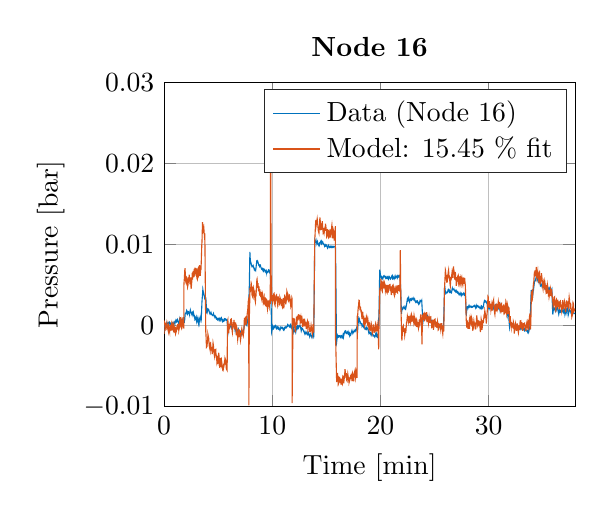
\begin{tikzpicture}

\begin{axis}[%
scaled y ticks = false,
 y tick label style={/pgf/number format/fixed,
/pgf/number format/1000 sep = \thinspace}, % Optional if you want to replace comma as the 1000 separator 
width=2.0556in,
height=1.62135in,
at={(1.011in,0.642in)},
scale only axis,
xmin=0,
xmax=38,
xlabel={Time [min]},
xmajorgrids,
ymin=-0.01,
ymax=0.03,
ylabel={Pressure [bar]},
ymajorgrids,
axis background/.style={fill=white},
title style={font=\bfseries},
title={Node 16},
legend style={legend cell align=left,align=left,draw=white!15!black}
]
\addplot [color=mycolor1,solid]
  table[row sep=crcr]{%
0.000833333333333333	-0.000818830449657984\\
0.01	0.000293887047898234\\
0.1175	-9.23886119253287e-05\\
0.169166666666667	0.000219937878788601\\
0.210833333333333	0.000186878250245617\\
0.2625	0.000377406109482642\\
0.264166666666667	0.000367836217009684\\
0.299166666666667	0.000196448142718311\\
0.3775	0.000322596725318952\\
0.438333333333333	9.4659286412252e-05\\
0.439166666666667	9.55292766370991e-05\\
0.483333333333333	0.000466145112413094\\
0.526666666666667	0.000411335728248516\\
0.6	8.59593841614631e-05\\
0.620833333333333	0.000161648533720929\\
0.650833333333333	7.00342130108278e-07\\
0.701666666666667	9.46592864151802e-05\\
0.776666666666667	0.000296497018571928\\
0.85	-6.25957966753077e-06\\
0.876666666666667	0.000227767790811531\\
0.883333333333333	0.000213847947213922\\
0.929166666666667	0.000433955474096637\\
1.0025	0.000246037585530212\\
1.04083333333333	0.000508774633428327\\
1.05166666666667	0.00049659477028112\\
1.09666666666667	0.000683642668622086\\
1.15083333333333	0.00049137482893262\\
1.22416666666667	0.000736712072337692\\
1.23083333333333	0.000758461827959814\\
1.315	0.000383496041056516\\
1.3375	0.000265177370478445\\
1.4025	0.00050007473118438\\
1.42166666666667	0.000679292717497448\\
1.44583333333333	0.000410465738022517\\
1.50416666666667	0.00029388704789679\\
1.56916666666667	0.000735842082110638\\
1.58833333333333	0.000749761925708414\\
1.64416666666667	0.000494854789829843\\
1.73	0.000783691544478812\\
1.7525	0.0005748938905175\\
1.76833333333333	0.000582723802542554\\
1.81333333333333	0.000423515591397861\\
1.86916666666667	0.00040698577712317\\
1.9275	0.00121868665688969\\
1.93583333333333	0.00117431715542442\\
1.95833333333333	0.0015223132453578\\
2.015	0.00149273357771525\\
2.08416666666667	0.00185986945259277\\
2.1125	0.00174242077223963\\
2.16166666666667	0.00140573455522568\\
2.19583333333333	0.00148316368523678\\
2.2225	0.00175460063538292\\
2.2775	0.00171806104594094\\
2.35583333333333	0.001337875317687\\
2.365	0.00148664364613293\\
2.42916666666667	0.0019312086510244\\
2.455	0.00178853025415546\\
2.54	0.00146837385141052\\
2.58583333333333	0.00130307570869914\\
2.62333333333333	0.00166151168132597\\
2.66666666666667	0.00172676094818454\\
2.69916666666667	0.00148577365591192\\
2.71583333333333	0.00158234257086928\\
2.7975	0.00107513826979937\\
2.81833333333333	0.00112211774193623\\
2.8475	0.000806311290324796\\
2.90416666666667	0.000979439345066571\\
2.97666666666667	0.000645363098723498\\
3.0025	0.000882870430102087\\
3.03083333333333	0.000490504838704844\\
3.11416666666667	0.000935069843604142\\
3.15333333333333	0.000495724780057966\\
3.2	0.000198188123164703\\
3.24	0.00064362311828145\\
3.2525	0.000492244819158966\\
3.27583333333333	0.000827191055720933\\
3.32833333333333	0.000640143157386711\\
3.40083333333333	0.00117605713587818\\
3.43833333333333	0.000898530254160729\\
3.50333333333333	0.00295170718474833\\
3.58333333333333	0.00446114022481266\\
3.59083333333333	0.00440372086997454\\
3.67416666666667	0.00386084696968721\\
3.68083333333333	0.00388607668620619\\
3.7525	0.00340062214076409\\
3.78	0.00350763093841419\\
3.835	0.00321009428153159\\
3.85666666666667	0.00350067101661904\\
3.94166666666667	0.00158234257086644\\
3.96666666666667	0.00153797306939833\\
4.02083333333333	0.00193468861192482\\
4.0375	0.00186334941348573\\
4.08	0.00205474726294778\\
4.12583333333333	0.00199384794721565\\
4.20416666666667	0.0015849525415423\\
4.2525	0.00142835430107521\\
4.335	0.00166586163244954\\
4.37916666666667	0.00142835430105888\\
4.44666666666667	0.0012995957477774\\
4.49416666666667	0.00124826632450988\\
4.54916666666667	0.00140747453566274\\
4.56583333333333	0.00149708352882283\\
4.64166666666667	0.00116735723360546\\
4.68166666666667	0.00120389682304745\\
4.6925	0.00108731813291496\\
4.72916666666667	0.0011708371944938\\
4.81666666666667	0.000865470625572975\\
4.82166666666667	0.000854160752647146\\
4.86583333333333	0.000979439345028199\\
4.90583333333333	0.00086982057670508\\
4.935	0.000726272189605873\\
5.0175	0.00086547062557725\\
5.07916666666667	0.000666242864091199\\
5.11166666666667	0.000879390469178926\\
5.19416666666667	0.000660152932531272\\
5.245	0.000934199853337647\\
5.295	0.000997709139761979\\
5.335	0.000725402199396222\\
5.34333333333333	0.000740192033223189\\
5.39	0.000522694476999111\\
5.44833333333333	0.000712352346008457\\
5.50166666666667	0.000526174437908769\\
5.51833333333333	0.000536614320612153\\
5.58166666666667	0.000794131427158049\\
5.60666666666667	0.000721052248262702\\
5.64666666666667	0.000850680791750283\\
5.71833333333333	0.00080892126096796\\
5.7375	0.000686252639269871\\
5.81083333333333	0.000755851857261236\\
5.8675	-8.86955034747061e-06\\
5.92166666666667	-0.000715301612902008\\
5.96333333333333	-0.000247246871955611\\
6.005	0.000114669061558853\\
6.04416666666667	4.50698435660729e-05\\
6.08583333333333	-0.000145458015660044\\
6.16166666666667	0.000132068866061666\\
6.2175	-0.000125448240488477\\
6.2275	-0.000227237096791164\\
6.28083333333333	-1.03963834408027e-06\\
6.35083333333333	3.28899804277333e-05\\
6.36416666666667	-7.32488269914039e-05\\
6.43083333333333	-4.80191104581945e-05\\
6.46166666666667	-0.00012805821114302\\
6.48916666666667	-6.10689638360223e-05\\
6.56833333333333	-0.000572623216029508\\
6.5725	-0.000622212658843643\\
6.605	-0.000434294770290541\\
6.72	-0.000429074828935991\\
6.74333333333333	-0.00058045312805706\\
6.74583333333333	-0.000570883235583214\\
6.78916666666667	-0.000747491251216162\\
6.8725	-0.00046822438905951\\
6.88833333333333	-0.000698771798631578\\
6.9275	-0.000669192130986179\\
6.96083333333333	-0.000862329960892402\\
7.02416666666667	-0.000852760068411437\\
7.0625	-0.00067615205278275\\
7.10583333333333	-0.000717911583587805\\
7.175	-0.00109809731181616\\
7.19	-0.00106329770282475\\
7.26833333333333	-0.000690941886611146\\
7.29083333333333	-0.00075358118279599\\
7.35583333333333	-0.000554353421315629\\
7.4425	0.00026952732157963\\
7.44583333333333	0.000235597702809232\\
7.52	0.000442655376314285\\
7.53166666666667	0.000393065933507269\\
7.61833333333333	0.000119019012683852\\
7.6525	2.85400293027482e-05\\
7.70583333333333	0.000496594770271877\\
7.79	0.00122303660799372\\
7.79333333333333	0.00121346671551988\\
7.88166666666667	0.00499183426196237\\
7.9325	0.0090920981915819\\
7.96916666666667	0.00809856935482327\\
8.05166666666667	0.00757570522971247\\
8.06166666666667	0.00759745498533317\\
8.13083333333333	0.00724597893451499\\
8.15666666666667	0.00725728880743515\\
8.23166666666667	0.00742432693060135\\
8.2325	0.00742606691105049\\
8.31916666666667	0.0070171715054077\\
8.3275	0.00709547062564053\\
8.3875	0.00691712262953144\\
8.46333333333333	0.00678488411536944\\
8.49416666666667	0.00710939046921948\\
8.57583333333333	0.00802636016616599\\
8.58333333333333	0.00803332008796827\\
8.65583333333333	0.00781843250243708\\
8.66916666666667	0.00787672184749692\\
8.75416666666667	0.0074652164711726\\
8.79583333333333	0.00749914608993589\\
8.8325	0.00729556837732059\\
8.9075	0.00743389682304819\\
8.93166666666667	0.00728077854345241\\
9.01916666666667	0.00698585185727763\\
9.07416666666667	0.00706415097747919\\
9.09166666666667	0.0069545322091447\\
9.10666666666667	0.0069780219452046\\
9.16333333333333	0.00675617443789389\\
9.19666666666667	0.0069014628054536\\
9.2175	0.00677966417397653\\
9.29083333333333	0.00692147258061238\\
9.35416666666667	0.00664742565979037\\
9.43	0.00679967394912108\\
9.45666666666667	0.0065708665199939\\
9.46833333333333	0.00671789486798713\\
9.5225	0.00655433670576468\\
9.55166666666667	0.00654302683282464\\
9.62666666666667	0.00677618421306687\\
9.635	0.00670919496577409\\
9.68166666666667	0.00682316368521226\\
9.7425	0.00661523602149469\\
9.7875	0.00678836407622367\\
9.825	0.0067161548875735\\
9.895	0.00262720083088408\\
9.94	-0.000746621260995145\\
10.0383333333333	-0.000151547947174493\\
10.065	-0.000379485386107659\\
10.0916666666667	-0.000408195063541991\\
10.15	-0.000171557722381574\\
10.1625	-0.000212447262944296\\
10.2166666666667	-7.41188172038998e-05\\
10.2516666666667	-0.000187217546445198\\
10.31	3.46299609195189e-05\\
10.3391666666667	-5.38958941508072e-06\\
10.3975	-0.000348165738031578\\
10.4775	-0.000174167693031843\\
10.5075	-0.000370785483840619\\
10.5608333333333	-0.000428204838689397\\
10.5941666666667	-0.000255946774185709\\
10.605	-0.000219407184738035\\
10.6833333333333	-0.00048040425219216\\
10.7066666666667	-0.000557833382211076\\
10.7708333333333	-0.000337725855322504\\
10.7941666666667	-0.000181997605050874\\
10.8775	-0.000305536217012611\\
10.9141666666667	-0.000186347556168753\\
10.9466666666667	-0.000216797214042289\\
11.0316666666667	-0.000538693597277581\\
11.0616666666667	-0.000576103176924955\\
11.0891666666667	-0.000369045503392895\\
11.1208333333333	-0.00040558509284909\\
11.145	-0.000222017155416726\\
11.2083333333333	-0.000281176490707538\\
11.2525	-0.000141108064471096\\
11.3233333333333	-0.000238546969645939\\
11.3833333333333	-3.49692570064813e-05\\
11.3983333333333	-4.80191103885697e-05\\
11.43	0.000148598680405995\\
11.4733333333333	8.59593842197359e-05\\
11.5566666666667	-0.000100218523916909\\
11.5983333333333	-0.000158507868990965\\
11.6391666666667	7.11695503558124e-05\\
11.6658333333333	0.000130328885652314\\
11.7208333333333	-0.00020983729226845\\
11.7475	-0.00026986661779875\\
11.8216666666667	6.94295699194686e-05\\
11.8258333333333	8.85693548700051e-05\\
11.905	-0.000969338758559563\\
11.9258333333333	-0.000985868572828563\\
11.97	-0.000239416959925229\\
11.9966666666667	-0.000329025953075365\\
12.065	-0.000723131524952292\\
12.1333333333333	-0.000652662316698693\\
12.1675	-0.000818830449648145\\
12.1716666666667	-0.000784030840659575\\
12.2483333333333	-0.000214187243428962\\
12.2891666666667	-0.000343815786916543\\
12.345	1.28802053130234e-05\\
12.3633333333333	2.15801075686972e-05\\
12.4108333333333	-0.000324676001943261\\
12.4383333333333	-0.000276826539603856\\
12.4941666666667	-2.01794232647795e-05\\
12.5533333333333	3.63699413558766e-05\\
12.6091666666667	-0.000131538172029932\\
12.6791666666667	-0.000650052346028537\\
12.7091666666667	-0.000504763978485867\\
12.7325	-0.000295096334306383\\
12.7983333333333	-0.000374265444767333\\
12.8716666666667	-0.000565663294227248\\
12.9575	-0.000841450195516874\\
12.9658333333333	-0.000804910606074891\\
13.0275	-0.00106155772241112\\
13.0508333333333	-0.00100500835778194\\
13.1116666666667	-0.00075793113392951\\
13.1416666666667	-0.000842320185773418\\
13.1908333333333	-0.000992828494716089\\
13.23	-0.000871029863204906\\
13.295	-0.00115116671557547\\
13.3141666666667	-0.00113724687197095\\
13.355	-0.000883209726316239\\
13.4025	-0.00103893797657366\\
13.46	-0.00135474442816662\\
13.485	-0.00123207580646426\\
13.5458333333333	-0.00102849809386174\\
13.5791666666667	-0.00118422634410212\\
13.6591666666667	-0.00144783338224345\\
13.665	-0.00146871314764173\\
13.7475	-0.00101805821116403\\
13.8308333333333	-0.00137475420337939\\
13.835	-0.0013434345552891\\
13.9225	0.00968456153468407\\
13.9333333333333	0.0106302409090891\\
14.0133333333333	0.0103579339686892\\
14.0875	0.0101978557673281\\
14.1116666666667	0.0103875136363147\\
14.1325	0.010121296627526\\
14.185	0.0103431441348623\\
14.2683333333333	0.00998731813292619\\
14.315	0.00986377952098717\\
14.3475	0.0100290776637199\\
14.36	0.00995860845552311\\
14.445	0.0103196543988137\\
14.4883333333333	0.0104240532257823\\
14.5325	0.0101935058162102\\
14.5516666666667	0.0102996446236436\\
14.5733333333333	0.0101369564516038\\
14.6591666666667	0.010337924193502\\
14.7041666666667	0.0101421763929299\\
14.7125	0.0101587062072103\\
14.7983333333333	0.00994729858259444\\
14.8041666666667	0.00996469838710294\\
14.845	0.00979244032260208\\
14.9058333333333	0.00996817834798987\\
14.9508333333333	0.00984115977518098\\
15.0091666666667	0.00992467883673424\\
15.0575	0.00975590073314589\\
15.0608333333333	0.00979766026393673\\
15.1258333333333	0.00958364266866493\\
15.1491666666667	0.00968282155426477\\
15.2116666666667	0.00991249897361723\\
15.2358333333333	0.00982636994135401\\
15.2958333333333	0.00964889193548157\\
15.38	0.00977330053763734\\
15.4075	0.0096497619257097\\
15.4241666666667	0.00963236212120688\\
15.4916666666667	0.00979418030302992\\
15.5075	0.00980723015639211\\
15.545	0.00964019203321169\\
15.5875	0.00967934159335794\\
15.6383333333333	0.00977330053765155\\
15.685	0.00968282155425908\\
15.7358333333333	0.00977765048873533\\
15.8016666666667	0.00976895058649671\\
15.8491666666667	0.00962366221895973\\
15.9366666666667	-0.00215513543500907\\
15.9383333333333	-0.00216731529816304\\
16.0233333333333	-0.00117117649076266\\
16.0241666666667	-0.00117378646143851\\
16.0816666666667	-0.00143739349955711\\
16.1116666666667	-0.00142434364617219\\
16.1458333333333	-0.00122424589445945\\
16.245	-0.00125034560121225\\
16.2833333333333	-0.00145392331379771\\
16.2891666666667	-0.00146349320626445\\
16.3641666666667	-0.00120858607040435\\
16.3791666666667	-0.00120945606064669\\
16.4608333333333	-0.00153396241450099\\
16.4616666666667	-0.00153309242427571\\
16.5416666666667	-0.00111984706744823\\
16.5816666666667	-0.00141042380255345\\
16.6366666666667	-0.00103284804497394\\
16.7175	-0.000671802101683341\\
16.7775	-0.000630912561083677\\
16.8	-0.000794470723368648\\
16.8125	-0.000753581182803095\\
16.8608333333333	-0.000937149120246825\\
16.9533333333333	-0.000765761045968413\\
16.9866666666667	-0.000986738563048165\\
17.0433333333333	-0.00105111783969636\\
17.0683333333333	-0.000896259579692638\\
17.075	-0.00096324882699679\\
17.1416666666667	-0.00121902595309638\\
17.1733333333333	-0.000959768866112709\\
17.2466666666667	-0.00114942673508796\\
17.2508333333333	-0.00112680698924482\\
17.3283333333333	-0.000755321163247974\\
17.3683333333333	-0.000571753225781499\\
17.425	-0.0008327502932612\\
17.4508333333333	-0.000961508846549067\\
17.5108333333333	-0.000774460948192821\\
17.5366666666667	-0.000789250781988535\\
17.5666666666667	-0.000602202883635133\\
17.6491666666667	-0.000710081671590104\\
17.6708333333333	-0.000552613440876426\\
17.695	-0.000600462903255619\\
17.775	-0.000364695552263636\\
17.795	-0.000281176490673427\\
17.8616666666667	-0.000753581182757618\\
17.875	-0.000878859775144347\\
17.95	0.000483544916901169\\
18.005	0.000980309335350107\\
18.0491666666667	0.000842850879812257\\
18.1008333333333	0.000403505816214927\\
18.125	0.000487024877842093\\
18.2116666666667	0.000206018035178029\\
18.2691666666667	0.000247777565980239\\
18.2916666666667	2.76700391087237e-05\\
18.3033333333333	8.76993645850394e-05\\
18.3825	-7.41188172607432e-05\\
18.405	6.8559579634489e-05\\
18.4758333333333	-0.000260296725329165\\
18.5175	-0.000221147165225546\\
18.55	-0.000331635923756887\\
18.5758333333333	-0.000219407184780668\\
18.6375	-0.000443864662767232\\
18.6608333333333	-0.000472574340127666\\
18.7191666666667	-0.000259426735103888\\
18.7433333333333	-0.000396015200365293\\
18.7975	-0.000288136412566642\\
18.8258333333333	-0.000295096334380282\\
18.9083333333333	-0.000776200928597912\\
18.9216666666667	-0.000663102199379359\\
18.985	-0.000886689687061057\\
19.0375	-0.00083101031269979\\
19.0541666666667	-0.000966728787787072\\
19.09	-0.000908439442681749\\
19.1458333333333	-0.00119031627554836\\
19.1758333333333	-0.00109983729215304\\
19.2241666666667	-0.000888429667522991\\
19.27	-0.00101718822083074\\
19.3241666666667	-0.00125295557173462\\
19.3733333333333	-0.00118944628533445\\
19.4383333333333	-0.00132081480937489\\
19.4758333333333	-0.00140259389053443\\
19.5258333333333	-0.00116421656884672\\
19.57	-0.000975428689994437\\
19.6116666666667	-0.00127731529798569\\
19.6525	-0.00133995459418333\\
19.6658333333333	-0.00108417746808658\\
19.7025	-0.00121206603120316\\
19.7483333333333	-0.00141651373401959\\
19.7933333333333	-0.00133821461376686\\
19.8766666666667	0.00219742565996381\\
19.9325	0.00691973260020728\\
20.0116666666667	0.00617241099696213\\
20.0516666666667	0.00599232302047067\\
20.0941666666667	0.00586704442818342\\
20.1308333333333	0.00604278245348593\\
20.1458333333333	0.0060192927174374\\
20.2141666666667	0.00577395547411226\\
20.2291666666667	0.00584007473113712\\
20.305	0.0061471812804403\\
20.33	0.00618111089921496\\
20.385	0.00604539242420725\\
20.4016666666667	0.00606888216028989\\
20.4791666666667	0.00587313435973766\\
20.515	0.006008852834734\\
20.5691666666667	0.00582180493644598\\
20.6025	0.00580440513196305\\
20.6508333333333	0.00600363289345052\\
20.7341666666667	0.00578178538616254\\
20.75	0.00598275312803236\\
20.7775	0.00605409232643735\\
20.8391666666667	0.00590967394912564\\
20.8458333333333	0.00596361334306476\\
20.9166666666667	0.00577656544481084\\
20.9316666666667	0.00575046573802962\\
21.015	0.00602886260995529\\
21.0775	0.00618807082100585\\
21.1	0.00598710307917014\\
21.1175	0.00606975215053791\\
21.1558333333333	0.00586965439885927\\
21.1908333333333	0.00599754296184511\\
21.2675	0.00576960552300858\\
21.2775	0.0058096250733318\\
21.3525	0.00613761138804177\\
21.3991666666667	0.00590880395892879\\
21.4491666666667	0.00603843250240499\\
21.4591666666667	0.0060271226295161\\
21.5233333333333	0.00613500141736591\\
21.5575	0.00588879418379275\\
21.6266666666667	0.00611151168126053\\
21.6366666666667	0.00614631129023775\\
21.6975	0.00599841295207039\\
21.7183333333333	0.00602451265881183\\
21.7483333333333	0.00618546085036979\\
21.8141666666667	0.00618111089928317\\
21.89	0.00378080786897823\\
21.94	0.00145967394912856\\
21.9775	0.0018937990712264\\
22.055	0.00216436603118705\\
22.0733333333333	0.00208954687186957\\
22.1525	0.00230878440851012\\
22.18	0.00236794374380093\\
22.2316666666667	0.00210520669593035\\
22.2741666666667	0.00205561725307786\\
22.3175	0.00225397502423204\\
22.3425	0.0021426162754072\\
22.4158333333333	0.00262807082108663\\
22.495	0.00336843250254656\\
22.5166666666667	0.00339975215070222\\
22.55	0.00317877463362816\\
22.6116666666667	0.00345804149577345\\
22.6783333333333	0.00299172673518097\\
22.695	0.00293082741942254\\
22.7658333333333	0.00327708352900555\\
22.7891666666667	0.00331101314775747\\
22.8475	0.00313788509300576\\
22.8608333333333	0.00312309525916458\\
22.9008333333333	0.0033258029816555\\
22.9408333333333	0.0032405439396062\\
23.0208333333333	0.00342759183788854\\
23.0283333333333	0.00337104247325652\\
23.0916666666667	0.0031926944770849\\
23.1533333333333	0.00331797306957111\\
23.2016666666667	0.00300999652995738\\
23.2533333333333	0.00290211774202231\\
23.2808333333333	0.00304392614873206\\
23.3375	0.00305871598255049\\
23.3658333333333	0.00293778734124754\\
23.4091666666667	0.00301086652017131\\
23.4216666666667	0.00286383817212123\\
23.4658333333333	0.00291168763450042\\
23.5508333333333	0.00260197111433381\\
23.5533333333333	0.00260545107523495\\
23.6416666666667	0.00300303660813239\\
23.6608333333333	0.00290472771268679\\
23.7175	0.00309699555242883\\
23.7441666666667	0.00311874530807228\\
23.8083333333333	0.00296910698935204\\
23.8191666666667	0.0030239163735335\\
23.9041666666667	0.000893310312878662\\
23.9283333333333	0.00046005518094358\\
23.9891666666667	0.00108122820152841\\
23.9916666666667	0.00107426827974319\\
24.0691666666667	0.00126827609978232\\
24.1266666666667	0.00126044618777751\\
24.1566666666667	0.00110993787888315\\
24.1675	0.00112559770294962\\
24.2225	0.000845460850556326\\
24.3233333333333	0.00116039731185293\\
24.3416666666667	0.000945509726338792\\
24.3641666666667	0.00104729858267416\\
24.4116666666667	0.000783691544572598\\
24.4333333333333	0.000908970136979229\\
24.4808333333333	0.000680162707763943\\
24.5341666666667	0.000513994574746282\\
24.57	0.000692342570878107\\
24.6233333333333	0.000869820576818767\\
24.675	0.000540964271821001\\
24.7408333333333	0.000619263392016872\\
24.7791666666667	0.000385236021483992\\
24.8058333333333	0.000423515591362333\\
24.84	0.000258217448581316\\
24.8691666666667	0.000385236021438515\\
24.89	0.000119889002875032\\
24.9741666666667	0.000453965249247235\\
25.0408333333333	0.000307806891467921\\
25.0466666666667	0.00032346671552301\\
25.13	0.000161648533722705\\
25.1391666666667	0.000236467693051565\\
25.2025	5.55097262609355e-05\\
25.28	0.000227767790776004\\
25.3033333333333	-0.000106308455499568\\
25.34	-0.000197657429171327\\
25.3875	6.07296675785296e-05\\
25.4025	8.07394427429775e-05\\
25.4458333333333	-0.000123708260045027\\
25.5108333333333	-4.51959924947787e-06\\
25.555	-0.000218537194566756\\
25.5908333333333	-8.28187194567287e-05\\
25.6533333333333	-0.000351645698898603\\
25.6591666666667	-0.000346425757569643\\
25.7166666666667	-0.000109788416440493\\
25.7425	-0.000214187243377809\\
25.7991666666667	-0.000408195063519259\\
25.8308333333333	-0.000242896920868985\\
25.9175	0.00427148235582746\\
25.9325	0.0049796543988553\\
26.005	0.00411401412514789\\
26.0158333333333	0.00412706397849871\\
26.0416666666667	0.0039469760019902\\
26.0983333333333	0.00404354491691135\\
26.1725	0.00418274335291113\\
26.2025	0.00412793396874674\\
26.2608333333333	0.00446462018569815\\
26.2758333333333	0.00448201999020949\\
26.3558333333333	0.00420971304991764\\
26.4	0.00435239144673898\\
26.4291666666667	0.00418361334311368\\
26.4575	0.00426800239487517\\
26.5025	0.00408965439883997\\
26.5591666666667	0.00404093494624687\\
26.6166666666667	0.00445331031281494\\
26.6425	0.00463078831867034\\
26.685	0.00441590073309368\\
26.7325	0.00441764071355562\\
26.7883333333333	0.00454117932550031\\
26.7933333333333	0.00450724970671997\\
26.8758333333333	0.00427235234605843\\
26.9266666666667	0.0043367316226043\\
26.9533333333333	0.00420101314752838\\
27.005	0.00432281177902251\\
27.0516666666667	0.00411749408602628\\
27.0975	0.00404963484856791\\
27.1325	0.00421580298142073\\
27.1533333333333	0.0041949232159912\\
27.2308333333333	0.00393392614861096\\
27.25	0.00396872575759954\\
27.285	0.00379646769312426\\
27.3633333333333	0.00385910698927074\\
27.3783333333333	0.003998305425208\\
27.4575	0.00372773846536671\\
27.4925	0.00392522624639224\\
27.5116666666667	0.00384518714578559\\
27.5325	0.00392783621711924\\
27.6141666666667	0.00380516759532025\\
27.6441666666667	0.00394436603131436\\
27.7	0.00404354491689997\\
27.7566666666667	0.00383648724345886\\
27.765	0.00380603758559102\\
27.8125	0.00392957619744476\\
27.8483333333333	0.00388868665684509\\
27.9316666666667	0.00135440513192617\\
27.9341666666667	0.00134831520034918\\
28.0125	0.00232792419338108\\
28.0666666666667	0.00236098382194183\\
28.1066666666667	0.00221656544461309\\
28.1075	0.0022104755130361\\
28.19	0.00251410210155752\\
28.1941666666667	0.00250192223840355\\
28.26	0.00227398479950448\\
28.3383333333333	0.00239752341143214\\
28.365	0.00231139437915755\\
28.4175	0.00226876485810731\\
28.43	0.00239056348959008\\
28.4833333333333	0.00238621353846366\\
28.5166666666667	0.00228616466260161\\
28.545	0.00230878440845896\\
28.6283333333333	0.00245755273694823\\
28.6825	0.00250627218952996\\
28.7016666666667	0.00242449310837611\\
28.7191666666667	0.00245233279558517\\
28.7983333333333	0.00219307570858729\\
28.8066666666667	0.00223918519051022\\
28.8575	0.00249496231661266\\
28.8975	0.00230008450619476\\
28.9725	0.00249061236550897\\
28.9916666666667	0.00249148235574563\\
29.055	0.00228355469199397\\
29.11	0.002366203763339\\
29.1575	0.00224962507316247\\
29.1875	0.00226354491673288\\
29.2083333333333	0.00208171695977381\\
29.2775	0.00210433670571075\\
29.3025	0.00230965439876382\\
29.3325	0.00218089584545038\\
29.3608333333333	0.00236533377310234\\
29.455	0.00214348626571205\\
29.5066666666667	0.00238969349938753\\
29.5108333333333	0.00238534354827248\\
29.595	0.00303087629536418\\
29.6191666666667	0.00308394569910643\\
29.6508333333333	0.00292908743901744\\
29.6925	0.00291777756599783\\
29.7333333333333	0.00303522624641102\\
29.775	0.00294996720440151\\
29.8575	0.00269332008795442\\
29.925	0.00213304638315645\\
29.945	0.00222787531769524\\
30.0091666666667	0.00261676094815226\\
30.0325	0.00239056348966966\\
30.0608333333333	0.00211390659816613\\
30.13	0.00236533377314782\\
30.1925	0.00213826632439447\\
30.2133333333333	0.0021808958454788\\
30.2633333333333	0.00251845205274077\\
30.3008333333333	0.0025062721895186\\
30.375	0.00201820767338501\\
30.4025	0.00198079809377742\\
30.4683333333333	0.00232792419348339\\
30.4866666666667	0.00235315390997112\\
30.5233333333333	0.00211303660795222\\
30.575	0.00204169740955291\\
30.61	0.00251323211145728\\
30.6591666666667	0.0026028411045932\\
30.6925	0.00214000630495871\\
30.7516666666667	0.00223135527853384\\
30.775	0.00242188313775711\\
30.8641666666667	0.00243319301064031\\
30.9083333333333	0.0022504950634389\\
30.9175	0.00217480591385634\\
30.98	0.00238273357766484\\
30.9958333333333	0.00228964462364485\\
31.0508333333333	0.00188335918856848\\
31.1325	0.00250627218956408\\
31.165	0.00218002585519668\\
31.1741666666667	0.00223657521982869\\
31.2258333333333	0.00199471793738194\\
31.3075	0.00214348626578027\\
31.3266666666667	0.00198340806442485\\
31.3491666666667	0.00209389682297893\\
31.3716666666667	0.00189553905172243\\
31.4558333333333	0.00202255762460236\\
31.4816666666667	0.00183985967731001\\
31.5216666666667	0.00194947844563882\\
31.5533333333333	0.00220960552285629\\
31.6091666666667	0.00209389682298462\\
31.67	0.00178940024432318\\
31.7008333333333	0.0018868391494696\\
31.7325	0.00140225459432809\\
31.8166666666667	0.00233488411526292\\
31.8716666666667	0.000888960361678362\\
31.9291666666667	-0.000135888123153502\\
31.9866666666667	0.000437435435012332\\
32.0458333333333	0.000274747262884428\\
32.0825	0.000293017057626743\\
32.1333333333333	3.63699413331309e-05\\
32.1341666666667	3.9849902234268e-05\\
32.195	0.000240817644155247\\
32.2258333333333	0.000203408064479452\\
32.3091666666667	2.59300584990046e-05\\
32.3508333333333	-0.000176777663844122\\
32.4375	7.55195014253834e-05\\
32.4816666666667	-0.000115008357803564\\
32.4858333333333	-7.41188172152657e-05\\
32.5716666666667	-0.000220277174977523\\
32.58	-0.000151547947225647\\
32.6258333333333	-0.000464744428100114\\
32.6741666666667	-0.000400365151497398\\
32.7225	-0.000132408162309222\\
32.7491666666667	-0.000212447262978407\\
32.8208333333333	-0.000436034750705569\\
32.8375	-0.000394275219960202\\
32.8841666666667	-0.000233327028356767\\
32.925	-0.00032641598238814\\
32.9841666666667	-0.00047518431078078\\
33.0183333333333	-0.000380355376264727\\
33.0616666666667	-0.00016981774193385\\
33.11	-0.000307276197500136\\
33.1725	-0.00052651373405542\\
33.2041666666667	-0.000504763978434714\\
33.2591666666667	-0.000279436510302447\\
33.2891666666667	-0.000378615395916479\\
33.3208333333333	-0.000576103176896534\\
33.3608333333333	-0.000446474633420332\\
33.4425	-0.000645702394856645\\
33.4983333333333	-0.000659622238410013\\
33.5266666666667	-0.000529993694967909\\
33.5391666666667	-0.000529993694967909\\
33.6116666666667	-0.000811870527754929\\
33.6575	-0.000661362218889003\\
33.695	-0.000804040615750123\\
33.7116666666667	-0.000693551857230149\\
33.7783333333333	-0.000270736608060984\\
33.8158333333333	-0.000340335826026772\\
33.885	0.00242449310852959\\
33.9358333333333	0.00439676094827388\\
34.0316666666667	0.00347196133933249\\
34.055	0.00359375997076979\\
34.06	0.00357114022495221\\
34.1433333333333	0.00455161920815254\\
34.1558333333333	0.00452290953071252\\
34.2358333333333	0.00540507961884241\\
34.2908333333333	0.00561213729232332\\
34.3233333333333	0.00558342761494583\\
34.4108333333333	0.00609933181814068\\
34.4308333333333	0.00614022135866077\\
34.4983333333333	0.0058505146139201\\
34.5791666666667	0.0053720199902703\\
34.6283333333333	0.0053502702346496\\
34.66	0.00556341783982117\\
34.7108333333333	0.00555645791804164\\
34.7608333333333	0.0051371226295235\\
34.775	0.00520498186710694\\
34.8133333333333	0.00500053416424504\\
34.8483333333333	0.00514669252209256\\
34.9358333333333	0.00480739633428907\\
34.9425	0.00477694667641555\\
35.0058333333333	0.0049552946725758\\
35.0266666666667	0.00496399457478315\\
35.1108333333333	0.00471778734106221\\
35.1916666666667	0.0045542291787886\\
35.1983333333333	0.00458293885622293\\
35.2858333333333	0.0048769955522435\\
35.29	0.0049074452101284\\
35.3258333333333	0.00468124775166853\\
35.3733333333333	0.00471865733140117\\
35.4575	0.00441764071347603\\
35.4616666666667	0.00444287043000924\\
35.525	0.00460642859232831\\
35.56	0.00445766026380494\\
35.6366666666667	0.00460816857272203\\
35.6383333333333	0.00461512849452429\\
35.7216666666667	0.00421493299113292\\
35.7358333333333	0.00423146280537919\\
35.8116666666667	0.00444983035182855\\
35.8441666666667	0.00453943934497016\\
35.8991666666667	0.00225832497555171\\
35.9341666666667	0.0013805048387074\\
35.9933333333333	0.00211999652984542\\
36.0125	0.00196078831877212\\
36.0991666666667	0.00214870620734228\\
36.1533333333333	0.00185116955031828\\
36.1616666666667	0.00189118910066992\\
36.2375	0.00234097404706728\\
36.2566666666667	0.0019955879276925\\
36.3366666666667	0.0023479339688468\\
36.3383333333333	0.0023522839199789\\
36.4183333333333	0.00181984990229904\\
36.4241666666667	0.00183202976540753\\
36.4825	0.00141878440854026\\
36.5166666666667	0.00164498186702286\\
36.5533333333333	0.00208171695997846\\
36.6266666666667	0.00169370131961596\\
36.6841666666667	0.00183202976545301\\
36.6975	0.00178157033232974\\
36.775	0.00207475703823302\\
36.7791666666667	0.002093896823212\\
36.815	0.00172937091890372\\
36.8941666666667	0.0018703093353086\\
36.9258333333333	0.00167543152486797\\
36.9925	0.00195904833832157\\
37.0375	0.00151883328445347\\
37.0466666666667	0.00142139437927864\\
37.125	0.00199210796674588\\
37.1308333333333	0.00207475703811934\\
37.1708333333333	0.0016032223363457\\
37.2133333333333	0.0018572594820601\\
37.2783333333333	0.0021130366081\\
37.3025	0.00195991832845022\\
37.3541666666667	0.00129437580642144\\
37.3875	0.00146228391988398\\
37.4558333333333	0.00197905811349738\\
37.475	0.00190771891499009\\
37.5558333333333	0.0017415507819781\\
37.6008333333333	0.00183637971648277\\
37.6108333333333	0.00166238167152852\\
37.6516666666667	0.00178853025415475\\
37.7075	0.00147011383183764\\
37.7375	0.00159539242431248\\
37.7933333333333	0.00189292908115458\\
37.8366666666667	0.00173198088955115\\
37.8808333333333	0.00148577365590409\\
38	0.0015205732648131\\
};
\addlegendentry{Data (Node 16)};

\addplot [color=mycolor2,solid]
  table[row sep=crcr]{%
0.000833333333333333	-0.00102189496608339\\
0.0108333333333333	0.000549560591616079\\
0.130833333333333	0.000244254857973151\\
0.1625	-0.000501906144537622\\
0.18	-0.000470814330594456\\
0.256666666666667	0.000319322455360866\\
0.271666666666667	0.000177722624725499\\
0.350833333333333	-0.00046069129716403\\
0.404166666666667	-0.000754023703468938\\
0.420833333333333	-9.47678401177999e-05\\
0.508333333333333	-0.00069277567482734\\
0.511666666666667	-0.000124192776212159\\
0.529166666666667	-0.000697259346058747\\
0.585	0.000122218603805916\\
0.630833333333333	-0.000617842199229081\\
0.690833333333333	9.85168898411392e-05\\
0.738333333333333	-0.000579658673329482\\
0.785833333333333	0.000108325808511434\\
0.800833333333333	0.000198634754059528\\
0.854166666666667	-0.000418236575299922\\
0.905	1.87604941544983e-05\\
0.941666666666667	-0.000727674362704281\\
0.994166666666667	-0.000818527518904671\\
1.0175	-0.000198135281068068\\
1.0525	-0.000238053647154075\\
1.0725	-0.000956411710027101\\
1.14416666666667	-0.000646291178784121\\
1.20916666666667	6.8725759393234e-05\\
1.23083333333333	-0.000484635682437731\\
1.25166666666667	0.000109143011102175\\
1.32666666666667	0.00015903615397426\\
1.36166666666667	-0.00060791094819693\\
1.415	-0.0002421171364637\\
1.4775	0.0009989156001468\\
1.505	0.000999237529473067\\
1.53333333333333	-6.370312278827e-05\\
1.59916666666667	-0.000275173055918521\\
1.61583333333333	0.000586548966681007\\
1.705	5.10771900903305e-05\\
1.74416666666667	0.00103604228387939\\
1.8275	-0.000365784217116175\\
1.8375	0.00534083407883731\\
1.845	0.00515608536636156\\
1.9225	0.00701746022502823\\
1.93666666666667	0.00702310150496927\\
2.01083333333333	0.00538176416041336\\
2.02916666666667	0.00530464912849667\\
2.06083333333333	0.00600515994498475\\
2.11666666666667	0.00589762948390643\\
2.17416666666667	0.00479466080022386\\
2.21333333333333	0.00503402431681833\\
2.27083333333333	0.00593915799051823\\
2.28666666666667	0.00543341030806468\\
2.32	0.00630713200639701\\
2.40333333333333	0.0051012727505605\\
2.435	0.00594962349145101\\
2.45833333333333	0.00565646607003166\\
2.50083333333333	0.00454027894495633\\
2.54166666666667	0.00508537165431632\\
2.6125	0.00653424486626509\\
2.63666666666667	0.00569786205512172\\
2.685	0.00675391139053474\\
2.7625	0.00600481992204433\\
2.78333333333333	0.00700583957016677\\
2.82	0.00617283186810188\\
2.84666666666667	0.00709172089741361\\
2.92083333333333	0.0070677101930983\\
2.9675	0.00618936052809555\\
2.9875	0.00706397081784779\\
3.03166666666667	0.00586391063065979\\
3.07583333333333	0.00572356374309204\\
3.12416666666667	0.0070276278094077\\
3.18666666666667	0.00717930166271188\\
3.2075	0.00618723564434362\\
3.26083333333333	0.00639963831924542\\
3.29083333333333	0.00746724159348718\\
3.33833333333333	0.00613683047593819\\
3.41333333333333	0.00729385081646232\\
3.41583333333333	0.0069243689488357\\
3.49833333333333	0.0104822549971946\\
3.50333333333333	0.0102494197357017\\
3.55166666666667	0.0127833575094516\\
3.59666666666667	0.0121463531310316\\
3.62	0.0114299923754679\\
3.67833333333333	0.0119690523125914\\
3.75583333333333	0.010597665319141\\
3.76833333333333	0.0113894683847649\\
3.85333333333333	-0.000832085942506738\\
3.85916666666667	-0.00061656727847624\\
3.9175	-0.00265766467403693\\
3.96583333333333	-0.0025633260521799\\
4.02416666666667	-0.00171019511857237\\
4.02916666666667	-0.00194044701325533\\
4.04916666666667	-0.00103349605698537\\
4.12833333333333	-0.00155734955504853\\
4.17083333333333	-0.00245273105321638\\
4.25833333333333	-0.00304071288251614\\
4.27	-0.00218537656706859\\
4.29583333333333	-0.0021366983185597\\
4.3575	-0.00307066050564884\\
4.38666666666667	-0.00262057830427705\\
4.46083333333333	-0.00351588784835764\\
4.4675	-0.00332993603099693\\
4.52666666666667	-0.00214099789340771\\
4.55583333333333	-0.00238275411556229\\
4.62666666666667	-0.00349035711815594\\
4.66	-0.00374817587692626\\
4.70166666666667	-0.00298727612096029\\
4.77833333333333	-0.00292035473220732\\
4.815	-0.00400585523247437\\
4.83833333333333	-0.00359285927078453\\
4.89166666666667	-0.00468216270118894\\
4.92166666666667	-0.00456040212121863\\
4.9375	-0.00376247640183704\\
4.99666666666667	-0.00433088085722773\\
5.04583333333333	-0.00334412853034153\\
5.08583333333333	-0.00375328459495688\\
5.145	-0.00507420967693862\\
5.16916666666667	-0.00504498091495142\\
5.195	-0.00406037033551219\\
5.28333333333333	-0.00400757417303149\\
5.29666666666667	-0.00486733678529457\\
5.34416666666667	-0.00461661169429652\\
5.43	-0.00553754285369673\\
5.4575	-0.0055592265658991\\
5.50833333333333	-0.00471515726741855\\
5.52083333333333	-0.00516296062010779\\
5.59666666666667	-0.00423482064657528\\
5.62333333333333	-0.0048134015910676\\
5.635	-0.00401096272614071\\
5.69583333333333	-0.00426812464614005\\
5.75583333333333	-0.00531442961412433\\
5.83	-0.00550966298108808\\
5.86	0.000479342792649771\\
5.89833333333333	0.000700785038650962\\
5.9475	-0.000457808431515115\\
5.98166666666667	-0.000934672213063289\\
6.02	0.00020825100112731\\
6.04916666666667	-0.000413397910065844\\
6.12833333333333	0.00043589420199584\\
6.1375	2.17437562382865e-06\\
6.15416666666667	0.000771373741481161\\
6.22083333333333	0.00082932105033572\\
6.295	-0.00070364335559684\\
6.31416666666667	-0.000857062316220357\\
6.39083333333333	0.000428636765323808\\
6.425	-0.000117266827351296\\
6.45583333333333	0.000724697410369475\\
6.48	0.000470048112499654\\
6.52	-0.000446828409514536\\
6.60083333333333	0.00039678888753527\\
6.65083333333333	-0.000605250129232396\\
6.67833333333333	-0.00119983547705455\\
6.72416666666667	-0.000268990227508128\\
6.745	-0.000404647161532277\\
6.8075	-0.00170842678600265\\
6.8475	-0.00133485067152614\\
6.9075	-0.000479913402449722\\
6.94333333333333	-0.00051423196196065\\
6.97	-0.00136591270556477\\
7.00583333333333	-0.000814934422732079\\
7.06166666666667	-0.00180968106079477\\
7.09333333333333	-0.00154231990943151\\
7.16666666666667	-0.000508349331304549\\
7.18583333333333	-0.000358406929251717\\
7.26583333333333	-0.00106906378617822\\
7.31583333333333	-0.00127301248735668\\
7.35333333333333	-0.000519635453606382\\
7.36583333333333	-0.000939206336000318\\
7.42416666666667	0.000964541338289386\\
7.4725	1.99558661673907e-05\\
7.53	0.00101559006163619\\
7.56333333333333	0.00106583055435725\\
7.61166666666667	0.000144131844400337\\
7.62583333333333	0.000396545541114527\\
7.705	0.00178809674626776\\
7.71166666666667	0.00150697342831563\\
7.79	0.00310355402441428\\
7.82583333333333	0.00331488624773775\\
7.83583333333333	-0.00982285091333435\\
7.8825	0.000986700268337568\\
7.9475	0.00466655064162745\\
7.975	0.00414639490585185\\
8.05	0.00526700538198543\\
8.05833333333333	0.00522603656619019\\
8.13333333333333	0.00376005895009837\\
8.16416666666667	0.00365091154458531\\
8.2	0.00466200577176647\\
8.2375	0.00478091201153776\\
8.2925	0.00366714384706746\\
8.36666666666667	0.00411857515498721\\
8.405	0.00319812090521389\\
8.44333333333333	0.00294577223522679\\
8.4775	0.00397413813844517\\
8.49583333333333	0.0036143959447058\\
8.57916666666667	0.00571325257735803\\
8.59333333333333	0.00577168942279209\\
8.66416666666667	0.00465221536599751\\
8.68083333333333	0.00525613420421824\\
8.73666666666667	0.00423112087863374\\
8.77083333333333	0.00483980581744085\\
8.84	0.00369867844551481\\
8.84416666666667	0.00449460585776469\\
8.92916666666667	0.0035336236531174\\
8.95416666666667	0.0041549922113277\\
8.9975	0.00344413979831569\\
9.0275	0.00324822131628734\\
9.08	0.00407005119756836\\
9.11166666666667	0.00394222887776554\\
9.17	0.00291104633215468\\
9.24166666666667	0.00340776318527303\\
9.255	0.00262140136800315\\
9.34833333333333	0.00349680347132416\\
9.35333333333333	0.00256024365971464\\
9.39916666666667	0.00248171500216732\\
9.43666666666667	0.00328326589097734\\
9.4825	0.00323047507672007\\
9.53	0.00244810572885519\\
9.55833333333333	0.00208828782201643\\
9.63166666666667	0.00304843799065102\\
9.68916666666667	0.00305519048131356\\
9.71833333333333	0.00237135893563083\\
9.72416666666667	0.00231700603557382\\
9.8075	0.00339612809763532\\
9.8175	0.00267599041101814\\
9.83583333333333	0.028439767127151\\
9.895	0.0065804337221787\\
9.95333333333333	0.00301665491986122\\
10.01	0.00376469802844722\\
10.0433333333333	0.00287479351889905\\
10.0725	0.00307368531331108\\
10.1266666666667	0.00391194163377095\\
10.1741666666667	0.00398971420846836\\
10.2275	0.00263888440720401\\
10.2608333333333	0.00251268724847427\\
10.3325	0.0036877959312058\\
10.3758333333333	0.00376896551142134\\
10.4058333333333	0.0031269189928445\\
10.43	0.00338105450215121\\
10.4875	0.00267919836367332\\
10.5533333333333	0.00360194506663594\\
10.5883333333333	0.00285328179119832\\
10.6175	0.00341152591848384\\
10.6358333333333	0.00257865399957735\\
10.7	0.00276039998004528\\
10.7058333333333	0.00352670275421194\\
10.7716666666667	0.00323663659320832\\
10.85	0.0024073802511145\\
10.8641666666667	0.00330789124738086\\
10.94	0.00225534912962112\\
10.9475	0.00223433488651816\\
11.0233333333333	0.00340342231835787\\
11.0725	0.00213504911111532\\
11.1108333333333	0.00313361351039871\\
11.1558333333333	0.00384172662720518\\
11.1941666666667	0.00280638634771847\\
11.2116666666667	0.00360583186274737\\
11.25	0.00264149741322102\\
11.3125	0.00324259871667248\\
11.3508333333333	0.00424919707926673\\
11.4108333333333	0.00395289321797551\\
11.4633333333333	0.0031351565636903\\
11.52	0.00299543276369012\\
11.5566666666667	0.00382904594845096\\
11.6058333333333	0.00378468206547334\\
11.64	0.00304852173622327\\
11.6466666666667	0.00345129093378034\\
11.715	0.00234000663496309\\
11.755	0.0025104624598121\\
11.8125	0.00342592046733825\\
11.8316666666667	0.00332060556057784\\
11.8358333333333	-0.00954513590066317\\
11.92	0.000960015719380748\\
11.9516666666667	3.48348966704418e-06\\
12.0341666666667	0.000889438287594216\\
12.0841666666667	-0.000319337957839707\\
12.1033333333333	9.04327158669079e-05\\
12.1308333333333	-0.000814505948728435\\
12.1716666666667	-0.0002049259720689\\
12.2358333333333	0.00111527221464206\\
12.2783333333333	0.000111741193426156\\
12.3358333333333	0.00124062064004589\\
12.3875	0.000655647934542273\\
12.4116666666667	0.00134868921558285\\
12.4858333333333	0.00131956531948127\\
12.4958333333333	0.000790509972731866\\
12.5358333333333	0.00128766053631348\\
12.5783333333333	0.000406116233468643\\
12.64	0.000969720410063172\\
12.6766666666667	0.000316713239994851\\
12.7341666666667	0.00122636294962511\\
12.78	0.000184585532078536\\
12.7966666666667	-0.00017676048450256\\
12.8191666666667	0.000609439738675035\\
12.8808333333333	0.000717915694340984\\
12.9091666666667	-8.29245374662701e-05\\
12.9866666666667	0.000862653805536772\\
13.0441666666667	-6.96170450003838e-05\\
13.0941666666667	0.000498030676384177\\
13.135	-0.000266162000973924\\
13.1383333333333	-0.000385320921539175\\
13.1466666666667	0.000390988137544621\\
13.23	-0.000300205042656134\\
13.2616666666667	0.000605512696336525\\
13.3266666666667	0.000382617411838533\\
13.3783333333333	-0.00023016102125962\\
13.3975	-2.07243240361735e-05\\
13.4641666666667	-0.000789531475857104\\
13.485	-0.000255423791287236\\
13.5033333333333	-0.00080292847388591\\
13.5875	5.09301127926834e-05\\
13.66	-0.000678308957507601\\
13.7008333333333	-0.00100947545228545\\
13.7475	-0.000212162565950329\\
13.7733333333333	0.000177750035111339\\
13.8308333333333	-0.00054753482823968\\
13.8358333333333	-0.000864101599525164\\
13.9225	0.0102846081459017\\
14.0033333333333	0.0126011491258339\\
14.03	0.0130521416473256\\
14.0633333333333	0.0124254119904911\\
14.1466666666667	0.0131377156712114\\
14.1841666666667	0.0125161352628946\\
14.1941666666667	0.0126332423591539\\
14.2583333333333	0.0117100210021534\\
14.3183333333333	0.0114109977547873\\
14.3558333333333	0.012184164899987\\
14.3608333333333	0.0120361129940964\\
14.4016666666667	0.013359097199208\\
14.45	0.0127692920770477\\
14.485	0.0118483118250966\\
14.5708333333333	0.0118967167331138\\
14.6108333333333	0.0128161924805908\\
14.6266666666667	0.012820783570908\\
14.71	0.0113492338180167\\
14.7391666666667	0.0113682363178073\\
14.7708333333333	0.0120315092872463\\
14.805	0.0115359006709681\\
14.88	0.0122176033596564\\
14.8858333333333	0.011707807843191\\
14.9183333333333	0.0125911395975362\\
14.9825	0.0119686313981364\\
15.0358333333333	0.0109279889167964\\
15.0766666666667	0.0110340449266553\\
15.1191666666667	0.0118156604433427\\
15.1766666666667	0.0117425472990629\\
15.225	0.010831492176688\\
15.26	0.0108908923522688\\
15.3233333333333	0.0117601172853727\\
15.3308333333333	0.0118798523319426\\
15.4033333333333	0.0109477090082024\\
15.4141666666667	0.010937042661391\\
15.4941666666667	0.0122271167461206\\
15.5125	0.0124039917640659\\
15.5858333333333	0.0109741541361247\\
15.5933333333333	0.0107864663138419\\
15.6408333333333	0.0118333685509727\\
15.6775	0.011632967669528\\
15.735	0.0104835865400111\\
15.8358333333333	0.012286690240629\\
15.8491666666667	-0.00180789469186116\\
15.855	-0.00139072773779534\\
15.935	-0.00606706464048531\\
15.9516666666667	-0.00695193341841925\\
16.0233333333333	-0.00602670912294299\\
16.035	-0.00583082813642256\\
16.0958333333333	-0.0072434462623123\\
16.1466666666667	-0.00704756713306565\\
16.1516666666667	-0.00633805480392705\\
16.2433333333333	-0.00644878577955205\\
16.2858333333333	-0.00702601293042595\\
16.3041666666667	-0.00658848438883548\\
16.3525	-0.00727799758437564\\
16.3791666666667	-0.00653004475862047\\
16.44	-0.00709105543782627\\
16.4716666666667	-0.00719984576758327\\
16.5233333333333	-0.00622042494050782\\
16.5508333333333	-0.0062669665423514\\
16.6041666666667	-0.00710673493010789\\
16.64	-0.00668493419711841\\
16.7241666666667	-0.00552914706654604\\
16.7283333333333	-0.00536202210444748\\
16.8116666666667	-0.00644367794832634\\
16.8383333333333	-0.00584890349081188\\
16.8775	-0.00671153963162251\\
16.9166666666667	-0.00681737023060491\\
16.9833333333333	-0.00594401881271514\\
16.9866666666667	-0.00597291240234206\\
17.0725	-0.00679568570068234\\
17.095	-0.00637862070333733\\
17.1091666666667	-0.00698119430528674\\
17.1641666666667	-0.00672928667387102\\
17.2466666666667	-0.00612323213669974\\
17.2525	-0.00659170009524872\\
17.3083333333333	-0.00592657772201866\\
17.3683333333333	-0.00684815356631074\\
17.4166666666667	-0.00580801443584718\\
17.4358333333333	-0.00588255496076691\\
17.5091666666667	-0.00680389505172694\\
17.5266666666667	-0.00680769649470594\\
17.5925	-0.00581275326683956\\
17.6475	-0.00551145759959053\\
17.6875	-0.00622465819892509\\
17.7041666666667	-0.00642045723737965\\
17.7525	-0.00573552307095981\\
17.8358333333333	-0.00643524536911584\\
17.86	0.00122760460867221\\
17.8741666666667	0.000866829324036695\\
17.9483333333333	0.00234398230827466\\
17.9516666666667	0.00206609726839161\\
18.0158333333333	0.00313856708798619\\
18.0383333333333	0.0031237190916257\\
18.1166666666667	0.00188287682597088\\
18.1483333333333	0.00233365468162216\\
18.2016666666667	0.00165982751868545\\
18.215	0.00196841941579622\\
18.295	0.000806260753639169\\
18.3566666666667	0.00172557129574263\\
18.3833333333333	0.00106483966032265\\
18.3916666666667	0.00133045215622529\\
18.44	0.000496889748782294\\
18.4783333333333	0.000785735012085378\\
18.5308333333333	0.000127719144811929\\
18.6058333333333	0.000996304910558279\\
18.6308333333333	0.00033435288837375\\
18.6941666666667	0.000509261651054812\\
18.7091666666667	0.00108734870421969\\
18.7466666666667	0.000898380140772697\\
18.7925	0.000359468487713775\\
18.835	0.000798444744079804\\
18.9091666666667	-5.1222042972531e-05\\
18.9541666666667	0.000414713818589049\\
18.9783333333333	-0.000215409428705594\\
19.0225	0.000128060150372166\\
19.0658333333333	-0.000540122906703129\\
19.0925	-0.000574286322371814\\
19.1616666666667	0.000125817604173671\\
19.1758333333333	-1.82936481908777e-05\\
19.2491666666667	-0.000925785187208292\\
19.2791666666667	-0.000734222076863611\\
19.3425	0.000162490093816536\\
19.3516666666667	-5.07043389654153e-07\\
19.4266666666667	-0.000823993405554985\\
19.4558333333333	-0.000801693012777177\\
19.5225	8.94754070581679e-05\\
19.5391666666667	0.000191016951659688\\
19.595	-0.000674944429629463\\
19.6275	-0.000656041428741487\\
19.7016666666667	0.000163037315412856\\
19.7875	-0.00079587363986498\\
19.8358333333333	-0.00290538473897396\\
19.8766666666667	0.00113536727356992\\
19.8783333333333	0.0011338067977478\\
19.9458333333333	0.00465383586949421\\
19.97	0.00428478411595604\\
20.0516666666667	0.00545316635288176\\
20.0533333333333	0.00576221792534558\\
20.1366666666667	0.00433435661894092\\
20.1675	0.00422895826737511\\
20.2116666666667	0.00537612993859163\\
20.2283333333333	0.00540601521431425\\
20.29	0.00468054321080865\\
20.315	0.00464338052123875\\
20.355	0.00537722746220025\\
20.435	0.00504259260049319\\
20.46	0.0043233477562005\\
20.5433333333333	0.00503610500819778\\
20.5633333333333	0.00418620252108822\\
20.6208333333333	0.00404243619966204\\
20.6458333333333	0.00502514436782927\\
20.7283333333333	0.00407486457143597\\
20.7441666666667	0.00489695776839987\\
20.7525	0.004334957870112\\
20.7808333333333	0.00498427827025226\\
20.88	0.00507030379183716\\
20.9133333333333	0.00429816465824861\\
20.93	0.00484102966560375\\
21.0016666666667	0.0038644622078399\\
21.03	0.00385347894937713\\
21.07	0.00479240293027687\\
21.1216666666667	0.00492053756552416\\
21.16	0.00406349045153234\\
21.2025	0.00453517381863875\\
21.2408333333333	0.00390270604329049\\
21.295	0.00369600174597778\\
21.305	0.0044732765458019\\
21.3716666666667	0.00415412849252995\\
21.4366666666667	0.00487722860703693\\
21.4533333333333	0.00488584685825138\\
21.4775	0.0041845740151498\\
21.5825	0.00403858664577827\\
21.5941666666667	0.00497758848655762\\
21.6875	0.00428811313340815\\
21.695	0.00493371191263985\\
21.765	0.00498797419972353\\
21.795	0.0041328599245543\\
21.8358333333333	0.00932204702290395\\
21.89	0.00213860919595007\\
21.8958333333333	0.00215677208857257\\
21.9708333333333	-0.00155577021857791\\
21.9808333333333	-0.0018465566537593\\
22.065	-0.000171887777755939\\
22.1141666666667	-1.75801691806136e-05\\
22.1483333333333	-0.000760854289475308\\
22.1766666666667	-0.000303381522776419\\
22.2391666666667	-0.00112948210039533\\
22.2433333333333	-0.00119516722741472\\
22.3275	-0.000277681166029573\\
22.3425	-0.000893972735209469\\
22.4133333333333	0.000400152988258285\\
22.4158333333333	0.00022389212062375\\
22.4891666666667	0.00118110171364325\\
22.5775	0.000590520061119102\\
22.5833333333333	0.00113806226245528\\
22.6258333333333	0.0011336807058367\\
22.6491666666667	0.000466319550958352\\
22.6866666666667	0.000417528006230857\\
22.7441666666667	0.000995159438380071\\
22.7908333333333	0.000456772586548466\\
22.8525	0.00108988158691458\\
22.8741666666667	0.00128406555951046\\
22.9366666666667	0.000562940685146628\\
22.9566666666667	0.000578278932819596\\
22.9841666666667	0.00124683090313004\\
23.0675	0.000485247245345494\\
23.11	0.00125783759450721\\
23.1225	0.00115735381453788\\
23.1925	0.000136645505226253\\
23.27	2.09396094145533e-05\\
23.2858333333333	0.000695483633917494\\
23.3075	0.000588348865283011\\
23.3783333333333	-1.93307470783967e-05\\
23.3925	-0.000180385142130026\\
23.3958333333333	0.000446151121458592\\
23.5108333333333	-0.000281468204016486\\
23.5416666666667	0.000433722126783456\\
23.5533333333333	1.75031220327059e-05\\
23.5941666666667	0.000775497668355268\\
23.6416666666667	0.000275482068038498\\
23.7258333333333	0.00138623017337186\\
23.7325	0.00121327908019647\\
23.8091666666667	-0.000121523295851919\\
23.8358333333333	-0.00230667385976502\\
23.8925	0.00136361762388539\\
23.9425	0.000701174149014833\\
23.9883333333333	0.00144442498964088\\
24.0258333333333	0.00153125881261997\\
24.0733333333333	0.000655752582021632\\
24.1075	0.00070957282277388\\
24.1541666666667	0.0016085736015212\\
24.1691666666667	0.00144803788284715\\
24.2408333333333	0.000943593211860595\\
24.2708333333333	0.00167069880055307\\
24.3391666666667	0.000436227897720948\\
24.4058333333333	0.00114737226663957\\
24.4275	0.000456756774043083\\
24.4383333333333	0.000325023883471034\\
24.495	0.00105369795914878\\
24.5516666666667	0.000343113285810459\\
24.6016666666667	0.00105135115346653\\
24.6475	0.00109356564558286\\
24.6816666666667	0.000246948207664508\\
24.7041666666667	0.000632726788481014\\
24.7433333333333	-0.000203903048258239\\
24.8008333333333	-0.000109677671919279\\
24.8333333333333	0.000744613401458995\\
24.8958333333333	-0.000526578926618049\\
24.9375	0.000356605901601863\\
24.9608333333333	-0.000197435661864496\\
24.9791666666667	0.000738386962032261\\
25.0441666666667	0.000814596553274541\\
25.11	-8.66017487256921e-05\\
25.1491666666667	-0.000137637190465888\\
25.1875	0.000508480669599931\\
25.2183333333333	-0.000239174003118636\\
25.2766666666667	0.000443029292296618\\
25.305	3.35532993920246e-05\\
25.3391666666667	-0.000535501463092209\\
25.395	-0.000423241436365252\\
25.4108333333333	0.000215940671907782\\
25.5091666666667	0.000131132134522574\\
25.5616666666667	-0.000396786341127288\\
25.5975	0.000298248990075376\\
25.6116666666667	-0.000399643070048378\\
25.6616666666667	0.000307950236517938\\
25.7425	-0.000866611384945562\\
25.7625	-0.0010392040491751\\
25.82	2.21779465127544e-05\\
25.855	-0.00069339143261539\\
25.9166666666667	0.00459177914264682\\
25.9208333333333	0.0045509610503784\\
26.0041666666667	0.00689651791290906\\
26.005	0.00689228081078075\\
26.0875	0.00583529729776539\\
26.135	0.00626353733161842\\
26.1641666666667	0.00532794422827663\\
26.1825	0.00548886793586551\\
26.2675	0.00664139787625931\\
26.2983333333333	0.00686978296720014\\
26.3483333333333	0.00581983278879503\\
26.3666666666667	0.00620264654707821\\
26.4375	0.00507869870525409\\
26.46	0.00489883339545155\\
26.5191666666667	0.00600389457351187\\
26.5316666666667	0.00563372637725964\\
26.6158333333333	0.00655308455024229\\
26.6766666666667	0.00586487457093755\\
26.705	0.00671758746302197\\
26.7608333333333	0.00730561803764681\\
26.7908333333333	0.00639721308686116\\
26.7958333333333	0.00683196079299998\\
26.8625	0.00569113945460539\\
26.9258333333333	0.00661867179698632\\
26.9675	0.00557545740844376\\
26.98	0.00599428845943137\\
27.0091666666667	0.00491776830595729\\
27.0558333333333	0.005305195408694\\
27.1375	0.00607644613440905\\
27.1883333333333	0.00622026287256238\\
27.22	0.00538917597211\\
27.3008333333333	0.00609056822842381\\
27.3108333333333	0.0052281228963077\\
27.3425	0.00503199629343092\\
27.4025	0.00580272869495844\\
27.4566666666667	0.0052740019492403\\
27.4891666666667	0.00587530008192479\\
27.515	0.00599451705575753\\
27.5816666666667	0.00521089592873821\\
27.6116666666667	0.0050300190515552\\
27.66	0.00588750514272693\\
27.7083333333333	0.00586479804652381\\
27.7358333333333	0.005159016404157\\
27.7841666666667	0.00588525783448991\\
27.8391666666667	0.00493295584693621\\
27.845	0.00516451883527121\\
27.93	0.000583914533024686\\
27.9341666666667	0.000862664204407667\\
27.9791666666667	-0.00024956185544644\\
28.025	0.000644360096719076\\
28.0983333333333	-0.000388959030943007\\
28.1083333333333	-0.00024019417910577\\
28.1916666666667	0.000462766362175716\\
28.2316666666667	-0.000404957815967174\\
28.2558333333333	0.000554807552530932\\
28.2858333333333	4.91159754818164e-05\\
28.2983333333333	0.000860065162349621\\
28.3816666666667	0.000390492482621473\\
28.3966666666667	0.00112757041677796\\
28.465	0.000828258469643381\\
28.535	-0.000547817680257464\\
28.5633333333333	-0.000524132099090012\\
28.62	0.000427119977062997\\
28.6358333333333	0.000615421196511741\\
28.7191666666667	-1.10238222213021e-05\\
28.7516666666667	0.000357306097029947\\
28.7866666666667	-0.00039307227304088\\
28.8175	-0.000377793082664757\\
28.8825	0.000912868312266268\\
28.9008333333333	0.00126955016396826\\
28.9658333333333	0.000280439401668234\\
29.0041666666667	0.000720853100615864\\
29.035	-6.90308558157095e-05\\
29.1008333333333	0.000642584408197923\\
29.1341666666667	-6.4939372661026e-05\\
29.1575	0.000525807563326633\\
29.2366666666667	-0.000793263541715629\\
29.2533333333333	-0.00055481408978863\\
29.3108333333333	0.000824233751476821\\
29.3358333333333	0.000653783119248402\\
29.3766666666667	-0.000511614942720089\\
29.42	-0.000126722181797876\\
29.4783333333333	0.000702733079279033\\
29.5091666666667	0.00031683548941114\\
29.5875	0.00144108313155308\\
29.6	0.000895866391195341\\
29.6466666666667	0.00184495657010978\\
29.6833333333333	0.00156046228063826\\
29.7566666666667	0.000781380552959578\\
29.7875	0.000271462302692361\\
29.8575	0.00156365964602807\\
29.8641666666667	0.00154964638501546\\
29.94	0.00360632780819704\\
29.9591666666667	0.00354807022075566\\
30.01	0.00224179302023442\\
30.0758333333333	0.00302309171133072\\
30.1141666666667	0.00219711109545103\\
30.135	0.00275371015229713\\
30.205	0.00204114354499546\\
30.2116666666667	0.00192811984427426\\
30.2883333333333	0.00262994240286676\\
30.3291666666667	0.00187230190657204\\
30.3783333333333	0.00272426344053374\\
30.4583333333333	0.00315490245053589\\
30.4708333333333	0.00245479250630738\\
30.475	0.00295648428079156\\
30.5516666666667	0.00157034693573829\\
30.5791666666667	0.00136871083126925\\
30.645	0.00250193240238316\\
30.6816666666667	0.00258532419936167\\
30.7275	0.00183385104697715\\
30.7475	0.00184712031952073\\
30.79	0.00265381361907722\\
30.8233333333333	0.00222278906132389\\
30.895	0.00299185252380561\\
30.9125	0.00281984115138158\\
30.9766666666667	0.0020900460585817\\
31.0041666666667	0.00292793940083759\\
31.08	0.001846147113312\\
31.1208333333333	0.00171132783126191\\
31.1633333333333	0.00271341081434197\\
31.1941666666667	0.00274867131445992\\
31.235	0.00175278068309022\\
31.2783333333333	0.00175557294422519\\
31.3191666666667	0.00239863899016775\\
31.3725	0.00249789567489059\\
31.4025	0.00178297534674051\\
31.48	0.00225052819499906\\
31.49	0.00153591255072336\\
31.5366666666667	0.00161335334618057\\
31.5908333333333	0.00285074511560467\\
31.6158333333333	0.00267306071458162\\
31.675	0.00145879159632662\\
31.7025	0.0016474757680794\\
31.7283333333333	0.00267042835812199\\
31.7858333333333	0.00232809708486631\\
31.8025	0.00143662822439036\\
31.8858333333333	0.00225116097151026\\
31.9466666666667	0.000359859132198535\\
32	0.00118075293011992\\
32.0383333333333	0.000134255248860851\\
32.085	-0.000221300283296322\\
32.1025	0.000465698010018933\\
32.1833333333333	-0.000238132503838477\\
32.2	0.000338492032251585\\
32.27	-0.000353587337584772\\
32.2916666666667	0.000480813853692949\\
32.3116666666667	0.00038844043903269\\
32.375	-0.000984276979753148\\
32.4016666666667	-0.000547022989359733\\
32.4775	0.000213577518866159\\
32.5616666666667	-0.000639024841613846\\
32.5658333333333	0.000152355707881279\\
32.6216666666667	-0.000617824600430043\\
32.6458333333333	0.00020565207444802\\
32.6766666666667	0.000170207591407556\\
32.7275	-0.00072245430832183\\
32.7516666666667	-0.00088941896581935\\
32.835	6.28802752916527e-05\\
32.8633333333333	-0.000505891059343652\\
32.9125	0.000591962930928016\\
32.9675	0.000614387894465231\\
32.9941666666667	-0.000189396870030774\\
33.0591666666667	-0.000334350452725442\\
33.0725	0.000428898963633235\\
33.1558333333333	-0.000630428372847541\\
33.1775	0.000289362605480675\\
33.2041666666667	-0.000408136697273441\\
33.2316666666667	0.000250102210361344\\
33.3225	0.000320199625177754\\
33.355	-0.000330136189357635\\
33.3841666666667	0.000113602912558714\\
33.4116666666667	-0.000581128132262527\\
33.4533333333333	-0.000583124263262663\\
33.5141666666667	0.000300918238634251\\
33.5466666666667	0.000485099887295907\\
33.6225	-0.000320946375764555\\
33.6325	-0.000475862995687626\\
33.6641666666667	0.000221729656974427\\
33.7116666666667	-0.000191507886036936\\
33.785	0.00124166964309065\\
33.8166666666667	0.00113157959636542\\
33.87	-0.000443917012368838\\
33.9	0.000286178925990242\\
33.9533333333333	0.00404251572832778\\
33.9833333333333	0.00415042422374462\\
34.01	0.00296961469874809\\
34.0641666666667	0.00361068373907861\\
34.1441666666667	0.00528185971319097\\
34.15	0.00489118241606443\\
34.2325	0.0066534246052245\\
34.2583333333333	0.00604448723389854\\
34.2741666666667	0.00682742812518725\\
34.3266666666667	0.0061071709480539\\
34.41	0.00723714408928863\\
34.4108333333333	0.00701482377884129\\
34.4508333333333	0.00601129928531301\\
34.5341666666667	0.00672813114076327\\
34.5641666666667	0.00590053912092195\\
34.62	0.00555423442058592\\
34.6475	0.0064300773201494\\
34.7033333333333	0.00660354788325052\\
34.7366666666667	0.00578301468090195\\
34.7758333333333	0.00611430599755734\\
34.7975	0.00536155769354767\\
34.8591666666667	0.00562050721431203\\
34.8808333333333	0.00647003362136257\\
34.9425	0.00575232727205837\\
35.0083333333333	0.00470662418531149\\
35.0308333333333	0.00451723036092896\\
35.1108333333333	0.00564761075343429\\
35.1191666666667	0.00567886059651311\\
35.1683333333333	0.00486137821910658\\
35.2108333333333	0.00520427881910799\\
35.285	0.00439473590252016\\
35.3358333333333	0.00500060635333838\\
35.3716666666667	0.00402728061800332\\
35.4083333333333	0.00405680489614212\\
35.44	0.00505233887957168\\
35.4633333333333	0.0048771634263765\\
35.5366666666667	0.00358608318637239\\
35.5625	0.00438486268775517\\
35.5925	0.00359258623269197\\
35.7008333333333	0.00445709940052801\\
35.7233333333333	0.00369495051150324\\
35.7341666666667	0.00425823887855117\\
35.7916666666667	0.0036361944266105\\
35.825	0.00449579512685627\\
35.8916666666667	0.00334726412323487\\
35.8991666666667	0.00356809297058659\\
35.9641666666667	0.00236584494981775\\
36.0091666666667	0.0026074249877471\\
36.0558333333333	0.00348977715336884\\
36.0916666666667	0.00354761478765662\\
36.1266666666667	0.00253584312354685\\
36.1733333333333	0.00213651890059518\\
36.2125	0.00302599862526998\\
36.2558333333333	0.00319612992888904\\
36.3066666666667	0.00233090592049978\\
36.3908333333333	0.00320541143505446\\
36.4233333333333	0.00232821145047983\\
36.4591666666667	0.00298187956602\\
36.4975	0.00207974184323523\\
36.5433333333333	0.00210443239450327\\
36.5816666666667	0.00293400964662238\\
36.6258333333333	0.00302746161611512\\
36.6858333333333	0.00234383321294669\\
36.6875	0.0025887063483453\\
36.7583333333333	0.00174883471872474\\
36.8125	0.00223343042511934\\
36.8391666666667	0.00314571380132887\\
36.9225	0.00203866130297522\\
36.935	0.00283656375944653\\
36.96	0.00235395384057341\\
37.0066666666667	0.00304607797785646\\
37.04	0.00288224653686611\\
37.1066666666667	0.0017513551154046\\
37.13	0.00177256266236488\\
37.2108333333333	0.00311320354116944\\
37.2641666666667	0.00229997924040163\\
37.2733333333333	0.00294289989816982\\
37.36	0.00227059815455293\\
37.3875	0.00300340017643138\\
37.3916666666667	0.00275956178227033\\
37.4425	0.00354023801184308\\
37.4766666666667	0.00320915870016193\\
37.5325	0.00206104449335934\\
37.5766666666667	0.00281059708186704\\
37.6333333333333	0.00178147208234125\\
37.6516666666667	0.00210848253419011\\
37.6891666666667	0.00108108388832589\\
37.7391666666667	0.00130673018106685\\
37.8	0.00284616452517443\\
37.8358333333333	0.00273114962416789\\
37.8691666666667	0.00174642902654207\\
38	0.00211011952173624\\
};
\addlegendentry{Model: 15.45 \% fit};

\end{axis}
\end{tikzpicture}% 
    \caption{Estimation comparison for node 16.}
  \end{minipage}
\end{figure}

\begin{figure}[H]
 \centering
    % This file was created by matlab2tikz.
%
%The latest updates can be retrieved from
%  http://www.mathworks.com/matlabcentral/fileexchange/22022-matlab2tikz-matlab2tikz
%where you can also make suggestions and rate matlab2tikz.
%
\definecolor{mycolor1}{rgb}{0.00000,0.44700,0.74100}%
\definecolor{mycolor2}{rgb}{0.85000,0.32500,0.09800}%
%
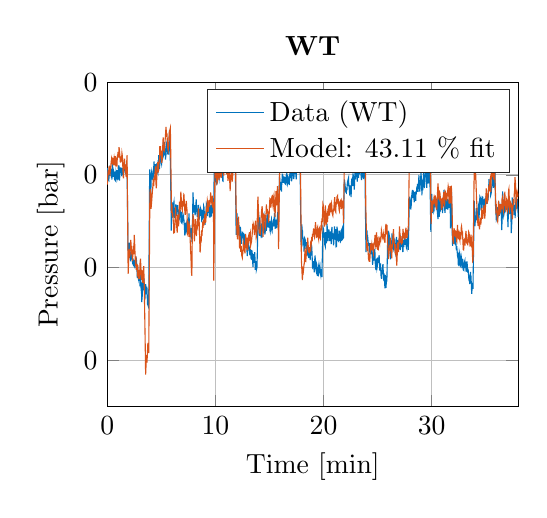
\begin{tikzpicture}

\begin{axis}[%
scaled y ticks = false,
 y tick label style={/pgf/number format/fixed,
/pgf/number format/1000 sep = \thinspace}, % Optional if you want to replace comma as the 1000 separator 
width=2.0556in,
height=1.62135in,
at={(1.011in,0.642in)},
scale only axis,
xmin=0,
xmax=38,
xlabel={Time [min]},
xmajorgrids,
ymin=-0.005,
ymax=0.002,
ylabel={Pressure [bar]},
ymajorgrids,
axis background/.style={fill=white},
title style={font=\bfseries},
title={WT},
legend style={legend cell align=left,align=left,draw=white!15!black}
]
\addplot [color=mycolor1,solid]
  table[row sep=crcr]{%
0.000833333333333333	8.51633431084853e-05\\
0.00833333333333333	0.000150412609970729\\
0.0816666666666667	-9.40546432063316e-05\\
0.143333333333333	-0.000117544379276413\\
0.168333333333333	8.34233626593184e-05\\
0.201666666666667	1.64341153476022e-05\\
0.26	0.000158242521994922\\
0.305833333333333	0.000127792864124399\\
0.343333333333333	-8.79560117406086e-06\\
0.375833333333333	0.000123442913000565\\
0.438333333333333	-0.0001027545454578\\
0.439166666666667	-7.83948191625805e-05\\
0.480833333333333	0.000205221994133087\\
0.546666666666667	0.000118222971652066\\
0.565	-4.01152492675305e-05\\
0.614166666666667	3.99238514169342e-05\\
0.696666666666667	-0.000111454447700943\\
0.731666666666667	7.47234604110136e-05\\
0.739166666666667	-0.000114934408601358\\
0.805833333333333	-0.000136684164220829\\
0.823333333333333	5.7323655914765e-05\\
0.904166666666667	-4.09852394930021e-05\\
0.931666666666667	0.00010430312805304\\
1.00083333333333	-0.000103624535678554\\
1.0375	0.000141712707722258\\
1.08416666666667	0.000207831964807531\\
1.135	-0.0001245043010768\\
1.14416666666667	-0.000100144574782024\\
1.21666666666667	0.000161722482890619\\
1.24666666666667	4.07938416402409e-05\\
1.315	0.000156502541546394\\
1.35333333333333	-3.14153470163114e-05\\
1.41916666666667	0.00015128260019398\\
1.46333333333333	3.64438905181008e-05\\
1.50833333333333	5.73236559149315e-05\\
1.54666666666667	0.000220881818184276\\
1.6075	0.000252201466277413\\
1.64166666666667	0.000102563147603707\\
1.695	1.64341153447711e-05\\
1.73416666666667	0.000192172140762392\\
1.79	0.000215661876830087\\
1.81833333333333	5.03637341123242e-05\\
1.84	7.82034213075156e-05\\
1.9275	-0.00163654731182694\\
1.9575	-0.00147037917888707\\
1.9975	-0.00179053558162812\\
2.06333333333333	-0.00146341925709653\\
2.10083333333333	-0.00176530586510201\\
2.15833333333333	-0.00186622473117726\\
2.18083333333333	-0.00165655708699564\\
2.19833333333333	-0.00182968514173953\\
2.27333333333333	-0.00164437722385946\\
2.2975	-0.00168439677419974\\
2.35333333333333	-0.00192712404692505\\
2.375	-0.00179488553275239\\
2.41166666666667	-0.00194191388075415\\
2.4925	-0.00196888357771588\\
2.5225	-0.00183490508308981\\
2.56166666666667	-0.00201847302053143\\
2.62083333333333	-0.00183142512218515\\
2.63	-0.00192886402736636\\
2.66	-0.00176269589442474\\
2.71916666666667	-0.00186361476051136\\
2.78666666666667	-0.00222814066472016\\
2.8175	-0.00197758347996801\\
2.88833333333333	-0.00222379071359588\\
2.96	-0.00210547204301781\\
2.9675	-0.00228816999022985\\
3	-0.00208807223851926\\
3.0325	-0.00240387869013778\\
3.10666666666667	-0.00215071153470978\\
3.135	-0.00250305757575964\\
3.16166666666667	-0.00239865874877754\\
3.19333333333333	-0.00274752482893481\\
3.245	-0.00260310645162026\\
3.26833333333333	-0.00231252971652074\\
3.3425	-0.00249261769305978\\
3.39916666666667	-0.00223597057673988\\
3.41916666666667	-0.00234558934506657\\
3.4825	-0.00269097546432623\\
3.51333333333333	-0.00257874672532088\\
3.55416666666667	-0.00235602922776357\\
3.63416666666667	-0.00258048670577216\\
3.6525	-0.0024125785923842\\
3.6825	-0.00245433812317292\\
3.7225	-0.00278493440860492\\
3.835	-0.00285888357772554\\
3.85333333333333	-0.00225598035191643\\
3.9275	0.000120832942317961\\
3.99333333333333	-0.000111454447713905\\
4.005	-0.000314162170098248\\
4.035	-0.000338521896390526\\
4.0875	3.81838709636872e-05\\
4.11833333333333	8.16833822107899e-05\\
4.20083333333333	-8.36147605013104e-05\\
4.25	-6.6214956008448e-05\\
4.28916666666667	0.000109523069397821\\
4.33416666666667	0.000289611045938998\\
4.37916666666667	5.81936461444832e-05\\
4.39	1.99140762576211e-05\\
4.45833333333333	0.000230451710646756\\
4.47416666666667	5.73236559149315e-05\\
4.55416666666667	0.000196522091886309\\
4.57333333333333	0.000247851515158104\\
4.64	7.55934506345146e-05\\
4.68916666666667	3.99238514320333e-05\\
4.72333333333333	0.000320930694040655\\
4.74416666666667	8.60333333378982e-05\\
4.76916666666667	0.000425329521002132\\
4.84083333333333	0.000125182893434439\\
4.89666666666667	0.000450559237515441\\
4.92416666666667	0.000543648191569546\\
4.98	0.000296570967729892\\
5.02666666666667	0.000239151612916641\\
5.07166666666667	0.000394009872933157\\
5.08416666666667	0.000374000097758759\\
5.16666666666667	0.000654136950139259\\
5.17	0.000702856402726687\\
5.19333333333333	0.000410539687187947\\
5.255	0.00046360909090179\\
5.27583333333333	0.000707206353861622\\
5.3425	0.000562787976548504\\
5.38666666666667	0.000333110557173305\\
5.45	0.00047056901268841\\
5.4875	0.000681106647100291\\
5.5325	0.000721126197459038\\
5.6025	0.000446209286401808\\
5.62333333333333	0.000632387194510031\\
5.6675	0.00043837937437427\\
5.69583333333333	0.000547128152484894\\
5.755	0.000932533822079154\\
5.78416666666667	0.000925573900283999\\
5.8675	-0.000103624535668589\\
5.92666666666667	-0.00120416217007308\\
5.96	-0.000818756500483075\\
6.00333333333333	-0.000589079081129179\\
6.08333333333333	-0.000923155327471559\\
6.12916666666667	-0.000636058553266039\\
6.17416666666667	-0.000576899217978072\\
6.21666666666667	-0.00087443587487418\\
6.24	-0.000930985239477766\\
6.305	-0.000751767253159036\\
6.35083333333333	-0.000629968621687627\\
6.3925	-0.000859646041048628\\
6.395	-0.000883135777118488\\
6.47916666666667	-0.000664768230686175\\
6.52	-0.000661288269780763\\
6.5675	-0.000841376246329073\\
6.58083333333333	-0.000756987194520664\\
6.61	-0.000983184652969177\\
6.66583333333333	-0.000954474975557562\\
6.69416666666667	-0.000753507233616696\\
6.77	-0.000770907038128044\\
6.82416666666667	-0.00101015434995436\\
6.85333333333333	-0.00102146422286598\\
6.91333333333333	-0.000798746725300142\\
6.92083333333333	-0.000813536559115757\\
6.9575	-0.000995364516104658\\
7.06083333333333	-0.000888355718450279\\
7.09166666666667	-0.00103538406645631\\
7.1025	-0.000970134799587075\\
7.17416666666667	-0.00129116119256442\\
7.1825	-0.00131117096773739\\
7.26166666666667	-0.00103277409581456\\
7.28666666666667	-0.00126419149560908\\
7.32666666666667	-0.00109367341151756\\
7.35666666666667	-0.00113804291298425\\
7.43916666666667	-0.000943165102634591\\
7.44333333333333	-0.000990144574774282\\
7.47666666666667	-0.00124505171064004\\
7.5625	-0.000829196383175107\\
7.61666666666667	-0.00117023255132542\\
7.625	-0.00108062355816532\\
7.685	-0.00133640068426777\\
7.72416666666667	-0.00133466070381436\\
7.745	-0.00115196275660015\\
7.84666666666667	-0.00145123939393688\\
7.87083333333333	-0.00102146422286598\\
7.88166666666667	-0.00109889335287353\\
7.93083333333333	-0.000375931476040037\\
7.97166666666667	-0.000594299022476624\\
8.01416666666667	-0.000815276539581938\\
8.07666666666667	-0.000655198338216589\\
8.125	-0.000872695894426456\\
8.1575	-0.000798746725315769\\
8.22833333333333	-0.000526439784937244\\
8.2325	-0.000594299022470934\\
8.31333333333333	-0.00085616608015035\\
8.33416666666667	-0.000911845454549975\\
8.4025	-0.000716097653975012\\
8.41833333333333	-0.000646498435997844\\
8.48666666666667	-0.00086312600195404\\
8.505	-0.000964914858249594\\
8.58166666666667	-0.000735237438905662\\
8.605	-0.000885745747785799\\
8.61666666666667	-0.000709137732141485\\
8.66916666666667	-0.000746547311814449\\
8.75083333333333	-0.0010258141739995\\
8.79166666666667	-0.000753507233622386\\
8.83083333333333	-0.000946645063538559\\
8.865	-0.000940555131958731\\
8.91916666666667	-0.000672598142708036\\
8.9475	-0.000700437829905698\\
9.01833333333333	-0.00100667438904897\\
9.04833333333333	-0.00107801358748238\\
9.1025	-0.000841376246324799\\
9.11	-0.000928375268807624\\
9.17083333333333	-0.000625618670556966\\
9.195	-0.000647368426186179\\
9.27583333333333	-0.000887485728244902\\
9.28416666666667	-0.000859646041052903\\
9.31833333333333	-0.000678688074290695\\
9.41916666666667	-0.000696087878802043\\
9.455	-0.000916195405690601\\
9.49166666666667	-0.000658678299137599\\
9.50333333333333	-0.000919675366577527\\
9.59333333333333	-0.000645628445761215\\
9.6325	-0.000897925610953976\\
9.7175	-0.000631708602148146\\
9.74	-0.000827456402751531\\
9.78333333333333	-0.000582119159361016\\
9.83333333333333	-0.000835286314781913\\
9.895	0.000110393059625929\\
9.9225	0.000414889638310101\\
9.97916666666667	-8.6224731208423e-05\\
10.0133333333333	-0.000159303910078179\\
10.0391666666667	3.557390030276e-05\\
10.0966666666667	-3.66352883758303e-05\\
10.1375	-0.000218463245369005\\
10.16	-0.000133204203339593\\
10.2291666666667	0.000103433137829345\\
10.3041666666667	0.000101693157373101\\
10.315	-5.66450635487992e-05\\
10.3408333333333	-9.14446725515938e-05\\
10.42	0.000136492766375895\\
10.4516666666667	0.000155632551334967\\
10.5058333333333	-2.53254154613525e-05\\
10.55	-3.75052786067975e-05\\
10.565	0.000169552394908234\\
10.5958333333333	0.000138232746823619\\
10.6833333333333	-0.000128854252190447\\
10.7025	-0.000133204203322523\\
10.7641666666667	0.000275691202324527\\
10.7866666666667	0.000346160410552548\\
10.8041666666667	0.000162592473125861\\
10.9175	0.000382699999994532\\
10.9291666666667	0.000225231769306444\\
10.9908333333333	0.000179992277605928\\
11.0333333333333	0.000345290420313046\\
11.0775	0.000392269892478328\\
11.1091666666667	0.000176512316738903\\
11.1433333333333	0.000358340273729246\\
11.1666666666667	0.000179122287431804\\
11.2491666666667	0.000398359824063832\\
11.2841666666667	0.000136492766395796\\
11.3325	2.60040078530754e-05\\
11.3775	0.000311360801575331\\
11.385	0.000153022580642065\\
11.4675	0.00046099912023588\\
11.5208333333333	0.000500148680339513\\
11.535	0.000360950244373826\\
11.5616666666667	0.000439249364618019\\
11.6041666666667	0.000258291397852967\\
11.6525	0.00027656119256686\\
11.7058333333333	0.000456649169112311\\
11.7408333333333	0.000377480058671248\\
11.7566666666667	0.00056278797655987\\
11.83	0.000527118377323277\\
11.9091666666667	-0.00106496373410597\\
11.9258333333333	-0.00129638113390901\\
11.9916666666667	-0.000819626490684205\\
11.9975	-0.00086312600193697\\
12.0575	-0.00109367341154032\\
12.0841666666667	-0.000933595210176358\\
12.1683333333333	-0.00122504193548698\\
12.1891666666667	-0.00108410351907073\\
12.225	-0.00133553069404957\\
12.2883333333333	-0.00138860009775205\\
12.3108333333333	-0.00111977311826753\\
12.3525	-0.00124244173999546\\
12.4083333333333	-0.0014903889540675\\
12.4341666666667	-0.0014146998044878\\
12.5025	-0.00122591192572363\\
12.5366666666667	-0.0013703303030268\\
12.5925	-0.00125462160310397\\
12.6091666666667	-0.00133727067446604\\
12.6758333333333	-0.00161392756596956\\
12.6975	-0.00151996862167028\\
12.7266666666667	-0.00134075063537001\\
12.7958333333333	-0.0013972999999935\\
12.8375	-0.00155911818180232\\
12.8733333333333	-0.00146167927663601\\
12.9533333333333	-0.00175225601170997\\
12.96	-0.00171223646135832\\
13.0191666666667	-0.00144862942324825\\
13.0525	-0.00144775943305139\\
13.13	-0.00164263724340674\\
13.1416666666667	-0.00155041827957508\\
13.1866666666667	-0.00173833616812535\\
13.2508333333333	-0.00160174770283267\\
13.2991666666667	-0.00180532541545222\\
13.3341666666667	-0.00181402531770222\\
13.3683333333333	-0.00162436744866729\\
13.4016666666667	-0.00167830684261208\\
13.4733333333333	-0.00198541339196642\\
13.5425	-0.00170440654935353\\
13.5708333333333	-0.00189580439882764\\
13.5725	-0.00189319442815181\\
13.6341666666667	-0.0016678669599286\\
13.6675	-0.00180967536656729\\
13.6866666666667	-0.00205153264906233\\
13.7666666666667	-0.00186361476051208\\
13.7883333333333	-0.00205066265886833\\
13.8491666666667	-0.00198976334312409\\
13.9225	-0.00117284252198135\\
13.9533333333333	-0.000701307820153735\\
14.0425	-0.000997104496579387\\
14.0758333333333	-0.00131552091885387\\
14.1075	-0.000917935386101382\\
14.125	-0.00123635180838721\\
14.1916666666667	-0.00129812111437946\\
14.2558333333333	-0.00104930391007929\\
14.3116666666667	-0.0013538004887379\\
14.3458333333333	-0.00107279364613636\\
14.4025	-0.00117632248290239\\
14.4433333333333	-0.000891835679388359\\
14.4825	-0.000859646041064255\\
14.5266666666667	-0.00113717292276466\\
14.5475	-0.00101363431083987\\
14.5716666666667	-0.00128681124146215\\
14.6233333333333	-0.00120677214076739\\
14.6566666666667	-0.000962304887551002\\
14.7175	-0.00120764213096994\\
14.76	-0.000889225708686936\\
14.8008333333333	-0.00087443587487418\\
14.8433333333333	-0.00113369296188059\\
14.8991666666667	-0.000937075171074664\\
14.965	-0.00114413284458398\\
15.02	-0.00099623450633704\\
15.0375	-0.0011911123166839\\
15.0691666666667	-0.00122330195500231\\
15.1091666666667	-0.00104843391982559\\
15.1683333333333	-0.000977094721417771\\
15.1866666666667	-0.00116849257089474\\
15.2425	-0.00121634203324836\\
15.3183333333333	-0.000999714467266599\\
15.3783333333333	-0.000970134799624045\\
15.4025	-0.00110933323559825\\
15.4141666666667	-0.00106148377323326\\
15.4658333333333	-0.000821366471154661\\
15.5008333333333	-0.000913585434986319\\
15.5241666666667	-0.00116240263927797\\
15.5941666666667	-0.000964044867990205\\
15.6483333333333	-0.0011389129032067\\
15.6758333333333	-0.00113804291297573\\
15.7575	-0.000814406549315444\\
15.7841666666667	-0.000816146529760337\\
15.8408333333333	-0.00113021300094818\\
15.8491666666667	-0.000897055620694587\\
15.925	-3.92452590317616e-05\\
15.955	-8.62247311487208e-05\\
15.9683333333333	-0.000330691984322479\\
16.0241666666667	-0.000149734017583003\\
16.1083333333333	-0.000359401661771036\\
16.1116666666667	-0.000285452492661764\\
16.1908333333333	8.60420332182699e-06\\
16.2341666666667	-4.44565005741637e-06\\
16.275	-0.000170613782969897\\
16.3391666666667	-3.40253176857597e-05\\
16.3666666666667	-0.000168873802542074\\
16.4083333333333	-4.70751710905937e-05\\
16.4258333333333	-0.000184533626631289\\
16.5191666666667	-0.000208023362657073\\
16.54	-2.09754643008264e-05\\
16.605	3.20939394101716e-05\\
16.6283333333333	-0.000140164125102066\\
16.6483333333333	-0.000163653861173341\\
16.6625	-1.22755620622084e-05\\
16.7275	-3.40253176857597e-05\\
16.7608333333333	-0.000188013587469893\\
16.8308333333333	-0.000200193450675012\\
16.8966666666667	8.69033234750793e-05\\
16.9141666666667	0.000108653079129883\\
16.9825	-6.70849462635625e-05\\
17.0158333333333	0.000153892570833231\\
17.0425	-0.000140164125187331\\
17.0991666666667	-4.44652004459867e-05\\
17.1275	0.000238281622617464\\
17.2208333333333	0.000186952199376922\\
17.2416666666667	-9.05746823348375e-05\\
17.2583333333333	-6.09950146695237e-05\\
17.325	0.000146932649070758\\
17.4066666666667	0.000245241544448146\\
17.42	6.51535679225823e-05\\
17.4725	-9.40546432075529e-05\\
17.5033333333333	0.000202612023477489\\
17.5141666666667	0.000133882795714246\\
17.5541666666667	0.000384439980476353\\
17.61	0.000260031378255227\\
17.6425	4.60137829606799e-05\\
17.7	0.000311360801563965\\
17.76	0.000106043108442672\\
17.8258333333333	0.000316580742898614\\
17.8625	-0.000464670479001839\\
17.9233333333333	-0.00150778875857033\\
17.9916666666667	-0.00106583372437105\\
18.0316666666667	-0.00126680146629771\\
18.0458333333333	-0.0011867623656342\\
18.0975	-0.00147994907138971\\
18.1658333333333	-0.00142252971654944\\
18.1891666666667	-0.00165307712611298\\
18.2183333333333	-0.00159478778107019\\
18.2733333333333	-0.00137816021509413\\
18.31	-0.00140686989248298\\
18.3816666666667	-0.00159652776159466\\
18.4083333333333	-0.00145210938425455\\
18.475	-0.00175660596284208\\
18.4808333333333	-0.00174529608991908\\
18.5583333333333	-0.00156172815254924\\
18.5733333333333	-0.0015573782013944\\
18.635	-0.00178444565001135\\
18.6858333333333	-0.00178270566967445\\
18.7183333333333	-0.00163567732165282\\
18.76	-0.00184012502443512\\
18.8233333333333	-0.00162523743894372\\
18.8325	-0.00173485620727254\\
18.8858333333333	-0.00152344858261974\\
18.9141666666667	-0.00156694809384977\\
18.9841666666667	-0.00200368318669736\\
19.0275	-0.00198802336266501\\
19.0675	-0.00186448475072032\\
19.1391666666667	-0.00210460205276763\\
19.1566666666667	-0.00189319442812053\\
19.2216666666667	-0.00173659618768329\\
19.2483333333333	-0.00198454340176388\\
19.315	-0.00206632248297456\\
19.3283333333333	-0.00189841436956317\\
19.3641666666667	-0.00192538406651854\\
19.4358333333333	-0.00212461182797188\\
19.4691666666667	-0.00218290117295783\\
19.5191666666667	-0.00200542316711949\\
19.5525	-0.00195583372432953\\
19.5791666666667	-0.00208894222874667\\
19.6633333333333	-0.00197149354837325\\
19.7008333333333	-0.00212287184745311\\
19.7433333333333	-0.00217333128051383\\
19.7841666666667	-0.00202804291302233\\
19.855	-0.00220552091884363\\
19.8766666666667	-0.00185056490713853\\
19.8833333333333	-0.00185317487780867\\
19.9366666666667	-0.00113282297169509\\
20.0041666666667	-0.00117371251224929\\
20.0158333333333	-0.00135119051814447\\
20.055	-0.00123722179871766\\
20.1033333333333	-0.00149995884659393\\
20.17	-0.00155215826004271\\
20.1866666666667	-0.00123722179865515\\
20.2633333333333	-0.00147907908119282\\
20.3141666666667	-0.00113978289346894\\
20.3258333333333	-0.00105191388076084\\
20.3825	-0.00137729022485178\\
20.4091666666667	-0.00142600967747331\\
20.465	-0.00118850234608478\\
20.5116666666667	-0.00119024232651829\\
20.5683333333333	-0.00141643978498385\\
20.6108333333333	-0.00141730977519205\\
20.6483333333333	-0.00121721202346795\\
20.7133333333333	-0.00149386891495443\\
20.7475	-0.00120155219942991\\
20.7741666666667	-0.0011206431085127\\
20.8208333333333	-0.00138425014664836\\
20.8441666666667	-0.00126419149561049\\
20.9133333333333	-0.00147385913986386\\
20.93	-0.00152170860223738\\
21.015	-0.00111803313784822\\
21.0158333333333	-0.00111194320627125\\
21.0508333333333	-0.00139903998046112\\
21.115	-0.00117284252204106\\
21.155	-0.00155302825025094\\
21.2	-0.00154345835777281\\
21.245	-0.00111890312805646\\
21.2908333333333	-0.00123026187681877\\
21.3283333333333	-0.00141295982403722\\
21.3966666666667	-0.00143296959923012\\
21.445	-0.00121547204304012\\
21.4641666666667	-0.0012172120234509\\
21.4958333333333	-0.00138599012706483\\
21.5508333333333	-0.00142339970674632\\
21.6158333333333	-0.00119981221904755\\
21.6441666666667	-0.00142948963838013\\
21.685	-0.00117806246343821\\
21.7433333333333	-0.00114152287395361\\
21.7733333333333	-0.00137903020526825\\
21.8391666666667	-0.00135554046928793\\
21.8891666666667	-0.00044031075277351\\
21.8958333333333	-0.000477720332449305\\
21.9216666666667	-9.66646139629601e-05\\
21.9841666666667	-0.000202803421390646\\
22.04	-0.000363751612965646\\
22.1016666666667	-0.000386371358794602\\
22.15	-0.000269792668714686\\
22.1633333333333	-0.000327212023515155\\
22.2033333333333	-0.000159303910126501\\
22.3133333333333	-5.92550343042342e-05\\
22.3225	-0.000244562952181476\\
22.3333333333333	-0.00017409374395061\\
22.4125	-0.000408991104691725\\
22.4291666666667	-0.000399421212224998\\
22.45	-0.000225423167208194\\
22.5466666666667	-0.00047772033236404\\
22.5908333333333	-0.000105364516147594\\
22.6258333333333	-8.88347018672131e-05\\
22.6766666666667	-0.000241952981443111\\
22.6783333333333	-0.000216723264921281\\
22.7141666666667	3.38339198124038e-05\\
22.7658333333333	-4.09852395334975e-05\\
22.8408333333333	-0.000316772140800392\\
22.8575	-0.00022020322583946\\
22.9008333333333	6.77635385700204e-05\\
22.96	-1.57555230116679e-05\\
23.0233333333333	0.000139102736980701\\
23.0433333333333	0.000113003030239256\\
23.1083333333333	-0.000146254056696105\\
23.1258333333333	-0.000113194428152386\\
23.1716666666667	0.000172162365541434\\
23.2316666666667	-6.36049853226517e-05\\
23.2841666666667	0.000113873020498645\\
23.3033333333333	1.90440860053376e-05\\
23.3758333333333	0.000276561192603803\\
23.4041666666667	0.000300050928680767\\
23.4583333333333	5.12424236670528e-06\\
23.5041666666667	-0.000112324438006683\\
23.5533333333333	7.90734114930192e-05\\
23.57	-5.75150537911462e-05\\
23.6041666666667	0.000215661876811268\\
23.6875	-8.97046921550237e-05\\
23.7275	0.000221751808365506\\
23.7341666666667	0.000112133040031021\\
23.8166666666667	0.000300920918809414\\
23.9041666666667	-0.00139382003909239\\
23.925	-0.00166438699899618\\
23.9541666666667	-0.00123200185726935\\
24.015	-0.00122069198435204\\
24.0375	-0.00139208005867023\\
24.0841666666667	-0.00135554046919129\\
24.1541666666667	-0.00153040850445041\\
24.1741666666667	-0.0014668992180332\\
24.2341666666667	-0.00160348768322638\\
24.3175	-0.00147559912018938\\
24.3408333333333	-0.00168526676439729\\
24.3466666666667	-0.00171571642225377\\
24.4241666666667	-0.0014790790811019\\
24.4291666666667	-0.00149908885628908\\
24.5075	-0.00180967536659571\\
24.5333333333333	-0.00193930391007191\\
24.6041666666667	-0.00175225601168155\\
24.6208333333333	-0.00161566754638603\\
24.6508333333333	-0.00184969491687345\\
24.74	-0.00159826774194291\\
24.7791666666667	-0.0019062442815623\\
24.8391666666667	-0.00205675259051918\\
24.8625	-0.00183751505384455\\
24.9208333333333	-0.00181750527863461\\
24.9441666666667	-0.00200281319654028\\
24.9641666666667	-0.00197584349953947\\
25.0283333333333	-0.00178531564028209\\
25.0516666666667	-0.00189754437930947\\
25.1158333333333	-0.00177748572827161\\
25.1366666666667	-0.00173224623659099\\
25.195	-0.00206284252199385\\
25.27	-0.00190972424243502\\
25.3008333333333	-0.00215767145653833\\
25.3533333333333	-0.00224119051813138\\
25.3925	-0.00205675259047372\\
25.41	-0.00214549159337299\\
25.4716666666667	-0.00194191388078754\\
25.4925	-0.00194104389059635\\
25.5541666666667	-0.00228208005868558\\
25.595	-0.00212809178889575\\
25.6508333333333	-0.00236385913983372\\
25.6791666666667	-0.00244998817205716\\
25.715	-0.00215854144671812\\
25.7708333333333	-0.00243606832847537\\
25.83	-0.00219595102642803\\
25.8516666666667	-0.00230382981425512\\
25.9175	-0.00147994907136129\\
25.9591666666667	-0.00120416217011712\\
26.0008333333333	-0.00157303802541539\\
26.0391666666667	-0.00157303802536424\\
26.0833333333333	-0.00131378093841183\\
26.0991666666667	-0.00133379071358763\\
26.165	-0.00173920615830231\\
26.1991666666667	-0.00182011524925929\\
26.2158333333333	-0.00141469980453326\\
26.2925	-0.00159043782990967\\
26.3266666666667	-0.00126332150538522\\
26.41	-0.00160522766376223\\
26.4333333333333	-0.00132161085042801\\
26.455	-0.00131639090909905\\
26.4816666666667	-0.00155911818181087\\
26.5691666666667	-0.00144949941355596\\
26.6183333333333	-0.00166351700885617\\
26.6541666666667	-0.00169918660801319\\
26.7016666666667	-0.00146080928637662\\
26.7441666666667	-0.00133727067450015\\
26.7933333333333	-0.00151648866082885\\
26.8608333333333	-0.00141121984365489\\
26.8741666666667	-0.00162262746829062\\
26.8933333333333	-0.00141556979475854\\
26.9416666666667	-0.00160087771255624\\
26.9758333333333	-0.00159043782990398\\
27.0033333333333	-0.00135554046924247\\
27.0866666666667	-0.00162349745848747\\
27.1175	-0.00133118074295158\\
27.1508333333333	-0.00134858054741177\\
27.2033333333333	-0.00155911818185633\\
27.2675	-0.00143470957971478\\
27.3141666666667	-0.00165394711638944\\
27.3416666666667	-0.00165220713592182\\
27.3858333333333	-0.00140686989251709\\
27.4091666666667	-0.00155563822094951\\
27.4925	-0.00130160107533744\\
27.4933333333333	-0.00131552091893061\\
27.5466666666667	-0.00150865874878425\\
27.6208333333333	-0.00138164017600662\\
27.6516666666667	-0.00157216803522989\\
27.7041666666667	-0.00160174770286109\\
27.7175	-0.00139643000980233\\
27.8091666666667	-0.0013103009774709\\
27.8416666666667	-0.00161914750729852\\
27.8441666666667	-0.00152344858257994\\
27.925	-0.000502080058671944\\
27.9333333333333	-0.000727407526917911\\
27.9625	-0.000469020430139633\\
28.0233333333333	-0.000570809286429497\\
28.0583333333333	-0.000745677321643157\\
28.1066666666667	-0.000648238416519481\\
28.1625	-0.000409861094848807\\
28.2166666666667	-0.000322862072377361\\
28.2575	-0.000501210068486468\\
28.2816666666667	-0.000335911925762294\\
28.3683333333333	-0.000548189540589217\\
28.3758333333333	-0.00059168905182494\\
28.4241666666667	-0.000367231573861093\\
28.5166666666667	-0.000560369403765915\\
28.5408333333333	-0.000357661681371635\\
28.57	-0.0004168210165999\\
28.6275	-0.000251522873898485\\
28.645	-0.00031242218968533\\
28.6783333333333	-0.00019323352890116\\
28.7325	-0.000363751612948604\\
28.8066666666667	-4.62051809306807e-05\\
28.8108333333333	-1.83567945830077e-06\\
28.8941666666667	-0.000361141642261392\\
28.895	-0.000353311730239531\\
28.98	-6.53449658130079e-05\\
29.0066666666667	6.77635385814002e-05\\
29.07	-0.000227163147630355\\
29.0908333333333	-0.000442920723392498\\
29.1191666666667	-0.000103624535725433\\
29.165	-0.000332431964804314\\
29.2358333333333	-9.65689153420435e-07\\
29.2483333333333	-1.83654936590782e-05\\
29.3183333333333	-0.000287192473214654\\
29.3383333333333	-0.000205413392077858\\
29.4008333333333	0.000154762561035776\\
29.4683333333333	0.000197392082057601\\
29.5075	-0.000146254056690415\\
29.5341666666667	-0.000276752590437357\\
29.5941666666667	3.03539589169566e-05\\
29.63	8.51633431097898e-05\\
29.6483333333333	-0.000174963734113381\\
29.7133333333333	-0.000172353763522787\\
29.7591666666667	0.00010952306938361\\
29.8075	8.95132942589361e-05\\
29.8575	-0.00039942121208289\\
29.9158333333333	-0.0012293918866276\\
29.945	-0.000743067350967297\\
29.9966666666667	-0.000408121114443716\\
30.0341666666667	-0.000585599120282054\\
30.0541666666667	-0.000823976441861773\\
30.1266666666667	-0.00058646911047322\\
30.1883333333333	-0.000788306842596759\\
30.2125	-0.000767427077224075\\
30.2616666666667	-0.000530789736089221\\
30.3225	-0.000683908015699231\\
30.3333333333333	-0.000543839589502576\\
30.4008333333333	-0.000676948093857183\\
30.4675	-0.000522089833773887\\
30.485	-0.000517739882658824\\
30.5191666666667	-0.000795266764359231\\
30.5741666666667	-0.000951865004927194\\
30.6033333333333	-0.000523829814332438\\
30.6575	-0.000444660703854433\\
30.6866666666667	-0.000903145552339779\\
30.7391666666667	-0.000774386999043392\\
30.77	-0.000513389931629055\\
30.8391666666667	-0.000694347898425374\\
30.9058333333333	-0.000580379178930363\\
30.9525	-0.000573419257139468\\
30.9958333333333	-0.000768297067517576\\
31	-0.000822236461456682\\
31.0833333333333	-0.000472500390983899\\
31.13	-0.000321992082089551\\
31.1683333333333	-0.000623878690160395\\
31.22	-0.000817886510307536\\
31.2408333333333	-0.000586469110507332\\
31.2625	-0.00074393734116418\\
31.3041666666667	-0.000449880645172041\\
31.3458333333333	-0.000471630400821155\\
31.3708333333333	-0.000736107429176402\\
31.4525	-0.000522959824124203\\
31.4791666666667	-0.000750027272803683\\
31.5233333333333	-0.000535139687249747\\
31.5891666666667	-0.000701307820182157\\
31.6283333333333	-0.000697827859286709\\
31.6725	-0.000509039980462839\\
31.6983333333333	-0.000548189540566457\\
31.7341666666667	-0.0011519627565888\\
31.815	-0.000286322482921153\\
31.8716666666667	-0.00110933323557266\\
31.875	-0.00110063333333121\\
31.9266666666667	-0.0015321484848555\\
31.985	-0.00123374183774833\\
32.0433333333333	-0.00142861964815486\\
32.0775	-0.00128507126105706\\
32.13	-0.0014799490713556\\
32.1533333333333	-0.00148864897357431\\
32.1925	-0.00130682101657545\\
32.23	-0.00145819931577468\\
32.2758333333333	-0.00162697741937723\\
32.3108333333333	-0.00153649843599898\\
32.3941666666667	-0.00177835571850257\\
32.4116666666667	-0.00167569687198171\\
32.4508333333333	-0.00193234398826395\\
32.4933333333333	-0.00194713382210512\\
32.5475	-0.00167569687202151\\
32.5783333333333	-0.00171658641258138\\
32.625	-0.0019445238514236\\
32.6708333333333	-0.00196888357768035\\
32.72	-0.00175399599221171\\
32.7466666666667	-0.00179227556211278\\
32.8191666666667	-0.0020089031281002\\
32.8575	-0.00181141534704626\\
32.9108333333333	-0.00205066265882853\\
32.9591666666667	-0.00206110254153191\\
32.9925	-0.00190624428155095\\
33.0591666666667	-0.00185143489740358\\
33.0708333333333	-0.00201064310853941\\
33.1508333333333	-0.00187057468227456\\
33.1725	-0.00207937233625149\\
33.1925	-0.00207763235581229\\
33.2558333333333	-0.00186622473121634\\
33.2725	-0.00190972424247482\\
33.3283333333333	-0.00210982199417051\\
33.36	-0.0020315228739064\\
33.4408333333333	-0.00228208005869124\\
33.4691666666667	-0.00216985131964681\\
33.5033333333333	-0.0023551592375127\\
33.5808333333333	-0.00209155219945092\\
33.6108333333333	-0.00228034007817246\\
33.6258333333333	-0.00217420127075049\\
33.6925	-0.00256569687195157\\
33.71	-0.00251175747800678\\
33.7775	-0.00233079951123888\\
33.8091666666667	-0.00245781808402787\\
33.885	-0.00130508103618174\\
33.9291666666667	-0.000562109384222159\\
33.9891666666667	-0.00110759325512777\\
34.0483333333333	-0.000922285337182305\\
34.0683333333333	-0.000975354740873402\\
34.1375	-0.000719577614981315\\
34.1516666666667	-0.000771777028475529\\
34.1941666666667	-0.000984054643274029\\
34.24	-0.000907495503437772\\
34.3233333333333	-0.000656068328461767\\
34.3241666666667	-0.000655198338242152\\
34.37	-0.000942295112358132\\
34.4116666666667	-0.000737847409479186\\
34.4475	-0.000465540469096387\\
34.5433333333333	-0.000512519941386708\\
34.5716666666667	-0.000769167057725784\\
34.6025	-0.000692607917900906\\
34.66	-0.000471630400849576\\
34.71	-0.00048033030302283\\
34.7541666666667	-0.00070217781036197\\
34.7883333333333	-0.00076481710646864\\
34.845	-0.00053600967727041\\
34.9	-0.000524699804449719\\
34.9341666666667	-0.000696957869055742\\
34.9358333333333	-0.000683038025462573\\
35.0225	-0.000455100586438467\\
35.0516666666667	-0.000630838611866025\\
35.0925	-0.000416821016526014\\
35.1291666666667	-0.000621268719427692\\
35.1983333333333	-0.000458580547350956\\
35.2058333333333	-0.000542969599152232\\
35.285	-0.000146254056480083\\
35.2875	-8.88347016341495e-05\\
35.3216666666667	-0.000301112316580449\\
35.4066666666667	-0.000149734017608594\\
35.4516666666667	-0.000438570772277463\\
35.4891666666667	-0.00040464115341754\\
35.5491666666667	-0.000252392863975964\\
35.56	-0.000255002834668866\\
35.6333333333333	5.12337243919747e-05\\
35.6366666666667	1.29541545022538e-05\\
35.7166666666667	-0.00028023255111681\\
35.7333333333333	-0.000237603030140476\\
35.8116666666667	-2.53254155238858e-05\\
35.8458333333333	0.00011474301070688\\
35.8966666666667	-0.000673468132921934\\
35.8991666666667	-0.000669118181812589\\
35.9666666666667	-0.000969264809313475\\
36.0033333333333	-0.000942295112369512\\
36.0666666666667	-0.000710007722406564\\
36.0825	-0.000712617693122197\\
36.15	-0.000862256011836759\\
36.1741666666667	-0.000831806353912057\\
36.2358333333333	-0.000649978396856349\\
36.2508333333333	-0.000884875757546311\\
36.3091666666667	-0.000648238416326219\\
36.3366666666667	-0.000672598142668235\\
36.3733333333333	-0.00083180635378699\\
36.4333333333333	-0.000685647996098632\\
36.4641666666667	-0.00119111231684588\\
36.5166666666667	-0.000910105474107942\\
36.5483333333333	-0.000355921700858519\\
36.6116666666667	-0.000682168035163411\\
36.6541666666667	-0.000873565884714267\\
36.6958333333333	-0.000820496480898103\\
36.7683333333333	-0.000595169012669206\\
36.7791666666667	-0.000602998924713827\\
36.8258333333333	-0.000736107429039984\\
36.9091666666667	-0.000623008699741856\\
36.9483333333333	-0.000749157282447649\\
36.9725	-0.000700437829877276\\
37.0358333333333	-0.00103799403700283\\
37.0433333333333	-0.00112934301064049\\
37.125	-0.0004986000976685\\
37.1275	-0.000442050733064914\\
37.18	-0.000845726197516578\\
37.2175	-0.000777866959944529\\
37.265	-0.0006673782012597\\
37.3066666666667	-0.000700437829809081\\
37.3483333333333	-0.00125549159327809\\
37.3975	-0.00103277409575345\\
37.4341666666667	-0.000487290224813725\\
37.4858333333333	-0.000783086901205265\\
37.505	-0.000659548289283302\\
37.5991666666667	-0.000661288269756616\\
37.6075	-0.00086834594327162\\
37.6883333333333	-0.000641278494637632\\
37.7058333333333	-0.000931855229734324\\
37.7375	-0.000736107429085475\\
37.79	-0.000484680254109443\\
37.8741666666667	-0.000727407526821267\\
37.9033333333333	-0.000523829814207399\\
38	-0.000904885532688027\\
};
\addlegendentry{Data (WT)};

\addplot [color=mycolor2,solid]
  table[row sep=crcr]{%
0.000833333333333333	0\\
0.0166666666666667	-0.00021037681260966\\
0.0891666666666667	0.00010816407365445\\
0.1325	-5.76350824981845e-06\\
0.176666666666667	0.000180555576958101\\
0.178333333333333	0.000193708917469507\\
0.264166666666667	3.38906781047926e-05\\
0.351666666666667	0.000234473653916821\\
0.3625	0.000218680388272567\\
0.410833333333333	0.000346873508553511\\
0.493333333333333	0.000233538048531683\\
0.51	0.000359260270764718\\
0.533333333333333	0.000356581642120336\\
0.558333333333333	0.000206959950815477\\
0.634166666666667	0.000356270972672881\\
0.694166666666667	0.000207765220052264\\
0.701666666666667	0.000241741276651686\\
0.74	0.000402175410485325\\
0.8025	0.000176974428974423\\
0.831666666666667	0.00031455271664392\\
0.908333333333333	0.000223064551669885\\
0.945	0.000431490981101331\\
0.965	0.000378112897701686\\
0.995	0.000497303919203063\\
1.05333333333333	0.00037421845093234\\
1.09666666666667	0.000599410299550012\\
1.14583333333333	0.000494946973712673\\
1.21416666666667	0.000277747419086418\\
1.25666666666667	0.000279129165985292\\
1.30333333333333	0.000399243877271615\\
1.31583333333333	0.000288546363773905\\
1.36416666666667	0.000470948526644814\\
1.4025	0.000410213579276399\\
1.485	-3.92091180903728e-05\\
1.5075	-7.32939855787159e-05\\
1.54666666666667	0.000248948442100896\\
1.60166666666667	0.000352478338982829\\
1.63333333333333	0.000129472280152008\\
1.665	0.000227177174861973\\
1.74833333333333	-4.26157613971882e-05\\
1.7525	5.62754599655864e-05\\
1.84	0.000428150184318422\\
1.9275	-0.0018766572144607\\
1.93916666666667	-0.00213559550951973\\
2.0125	-0.00166395809744896\\
2.02083333333333	-0.00160989684440337\\
2.0625	-0.00176306177891568\\
2.1025	-0.0017439396189056\\
2.17583333333333	-0.00140566615494171\\
2.19	-0.00143412384384767\\
2.2725	-0.00171364474448917\\
2.28833333333333	-0.00166407588984379\\
2.34083333333333	-0.0018607930091472\\
2.40666666666667	-0.00153108734128601\\
2.43916666666667	-0.00171602523595444\\
2.46083333333333	-0.0016451437956953\\
2.505	-0.00129747427550132\\
2.54416666666667	-0.00149862797047979\\
2.61416666666667	-0.00196380784198232\\
2.65583333333333	-0.00175899268815342\\
2.68666666666667	-0.00205060375938931\\
2.76916666666667	-0.00192740510194518\\
2.7925	-0.00217838319407122\\
2.82166666666667	-0.00195038762863467\\
2.85	-0.00220360090917489\\
2.90416666666667	-0.00222438122992168\\
2.96916666666667	-0.00205245254327631\\
2.995	-0.00224308815328536\\
3.03333333333333	-0.00191095550702397\\
3.07916666666667	-0.00180673938936691\\
3.15166666666667	-0.00218883169515733\\
3.19	-0.00226464457633798\\
3.20916666666667	-0.00205526149932809\\
3.29333333333333	-0.00233024169516393\\
3.31916666666667	-0.00213133810082833\\
3.37666666666667	-0.00197151054805712\\
3.415	-0.0022675045349081\\
3.41666666666667	-0.00225675673967608\\
3.50333333333333	-0.00349273253305628\\
3.50416666666667	-0.00348704412023221\\
3.55333333333333	-0.00431280904244787\\
3.63666666666667	-0.0038849772580563\\
3.67833333333333	-0.00404447228523021\\
3.67916666666667	-0.00405330901293942\\
3.76	-0.00362800259195647\\
3.84	-0.00384833152010491\\
3.85333333333333	-0.00348981490791391\\
3.94166666666667	-0.00052410897031224\\
3.97083333333333	-0.000300258163457713\\
4.02916666666667	-0.000418149770026879\\
4.055	-0.000730495732731674\\
4.11833333333333	-0.000551078646234404\\
4.20166666666667	-0.000279747448611013\\
4.20416666666667	-0.000304236089281678\\
4.26666666666667	-8.25607594633996e-05\\
4.29916666666667	-0.000239674260782196\\
4.36333333333333	-9.34464703834266e-06\\
4.37916666666667	-0.000112738109024113\\
4.4625	0.00018588103806757\\
4.46833333333333	0.000144132819879384\\
4.5275	-0.000287366838007533\\
4.55416666666667	-0.000234689368967298\\
4.62916666666667	0.000202162541978835\\
4.6775	0.000279898830759716\\
4.70416666666667	8.3084004622203e-05\\
4.73333333333333	7.36911239648361e-05\\
4.81666666666667	0.000333201613627098\\
4.84416666666667	0.000270573752362921\\
4.86333333333333	0.000610570120491433\\
4.925	0.000610031157775053\\
4.96666666666667	0.000417606245841954\\
4.99833333333333	0.000522680491999691\\
5.03916666666667	0.000253735577846328\\
5.08083333333333	0.000322048136802021\\
5.16666666666667	0.000781938645841322\\
5.17666666666667	0.000810063306455551\\
5.19666666666667	0.000567350289272967\\
5.26916666666667	0.000525571588063301\\
5.3425	0.000694995539659536\\
5.43	0.0010164916366801\\
5.43166666666667	0.00103427526903458\\
5.51	0.000821999873428118\\
5.52166666666667	0.000898217312163589\\
5.6025	0.000576909011715555\\
5.64	0.000529518539512831\\
5.6925	0.000681622975833459\\
5.69666666666667	0.000621935902121912\\
5.7275	0.000902843441519111\\
5.8375	0.00101222523989638\\
5.8675	0.000615166548132022\\
5.94166666666667	-0.000820346309291439\\
5.98416666666667	-0.000631814520362043\\
6.02333333333333	-0.000912486144654732\\
6.05166666666667	-0.000807804358086821\\
6.12916666666667	-0.00106343180237246\\
6.13916666666667	-0.00104520063754184\\
6.15666666666667	-0.00125263109967782\\
6.22416666666667	-0.0012411282666511\\
6.305	-0.000788849914185066\\
6.31583333333333	-0.000689030937519883\\
6.3925	-0.00102761603552397\\
6.39333333333333	-0.0010239176157228\\
6.47166666666667	-0.00124737989775819\\
6.48	-0.00119649936553854\\
6.525	-0.000855252133366838\\
6.6025	-0.0011100123120472\\
6.65583333333333	-0.000779712206055377\\
6.68166666666667	-0.000574658725908417\\
6.72583333333333	-0.000791650868975804\\
6.74666666666667	-0.000747148070836702\\
6.80916666666667	-0.000361289906621666\\
6.83416666666667	-0.000463144624384179\\
6.90916666666667	-0.000730909519169061\\
6.94916666666667	-0.000762473038556158\\
6.97166666666667	-0.000559592784840423\\
7.00666666666667	-0.000685260862126424\\
7.085	-0.000421654867780096\\
7.095	-0.000425603354182051\\
7.18	-0.000797865062616591\\
7.2125	-0.000860504882355263\\
7.2675	-0.000654794333174347\\
7.3175	-0.000560440401573776\\
7.355	-0.000744209024171737\\
7.3675	-0.000693361267313312\\
7.42583333333333	-0.00127180563689038\\
7.45	-0.00125468055293036\\
7.47416666666667	-0.000993403791023633\\
7.565	-0.00133440244365757\\
7.61333333333333	-0.00111106315193254\\
7.62916666666667	-0.00113299519635581\\
7.70583333333333	-0.00162121725108164\\
7.71416666666667	-0.0016144157794138\\
7.79333333333333	-0.00211151863779299\\
7.8275	-0.00217754522669063\\
7.87666666666667	-0.00104915008701514\\
7.89333333333333	-0.0011095463278836\\
7.92916666666667	-0.000844994844587551\\
7.97666666666667	-0.000939705948425369\\
8.05416666666667	-0.00139875310985887\\
8.0625	-0.0014343105349716\\
8.14416666666667	-0.000969274342897127\\
8.14666666666667	-0.000955420351786149\\
8.2025	-0.00119605570444536\\
8.245	-0.00132125085754403\\
8.31916666666667	-0.00103274883835368\\
8.36833333333333	-0.00109282015436049\\
8.40666666666667	-0.000813765572447145\\
8.445	-0.000722704871097289\\
8.49333333333333	-0.00098336777493375\\
8.4975	-0.000966247954292786\\
8.58166666666667	-0.00165662490883247\\
8.595	-0.00165878420625249\\
8.66916666666667	-0.00132502339541603\\
8.6825	-0.00145967991782086\\
8.74083333333333	-0.00119758928476393\\
8.75666666666667	-0.00131625351670562\\
8.84166666666667	-0.00100507828841054\\
8.85	-0.00114856909837466\\
8.93166666666667	-0.000958451411055923\\
8.95666666666667	-0.00109028162583188\\
8.99916666666667	-0.000925074960427601\\
9.03166666666667	-0.000838070686720529\\
9.08916666666667	-0.00101937997380906\\
9.115	-0.00101397537711114\\
9.17166666666667	-0.000688413747698826\\
9.21	-0.000750699937890311\\
9.25833333333333	-0.000556817922704873\\
9.29	-0.000607337711169634\\
9.32333333333333	-0.000796796420565359\\
9.37166666666667	-0.000681598261450703\\
9.40666666666667	-0.000543206023057513\\
9.48416666666667	-0.000682774356584559\\
9.54416666666667	-0.00047077995581966\\
9.56083333333333	-0.000378685257967124\\
9.6325	-0.00058038911777838\\
9.69083333333333	-0.000632331781807552\\
9.72	-0.000496139584704225\\
9.72583333333333	-0.000449568957371804\\
9.8075	-0.000716790328896607\\
9.82666666666667	-0.000585484315130586\\
9.84666666666667	-0.00228206156367886\\
9.895	-0.00142601564593884\\
9.955	5.75618975853451e-05\\
10	-7.07902340988058e-05\\
10.0575	0.000162057539032662\\
10.0766666666667	7.31642461039644e-05\\
10.145	-0.000179802652744407\\
10.18	-0.000158559763801467\\
10.2283333333333	0.000220113874986973\\
10.2625	0.000266316212974162\\
10.3325	-5.28915485311129e-05\\
10.34	-0.000104134999888349\\
10.39	2.6894975960984e-05\\
10.4208333333333	-1.86271946320141e-06\\
10.4891666666667	0.000192252758160261\\
10.5558333333333	-5.98884484895188e-05\\
10.5916666666667	0.000152336351995819\\
10.6183333333333	5.71691498495984e-05\\
10.6408333333333	0.000263948902336474\\
10.6833333333333	0.00021444503753112\\
10.77	-1.53134261254131e-05\\
10.7708333333333	-8.95616862362197e-06\\
10.8508333333333	0.00031131817582479\\
10.8666666666667	0.000152422401174542\\
10.9416666666667	0.00038900470361196\\
10.9491666666667	0.000413566666360773\\
11.0308333333333	1.16891367041462e-05\\
11.0333333333333	2.41644154236122e-05\\
11.085	0.000381378339981827\\
11.1208333333333	0.000135909682696695\\
11.1583333333333	-0.000129127289311696\\
11.2183333333333	-4.43486245045978e-05\\
11.255	0.000207903414198393\\
11.2958333333333	3.72999286560449e-05\\
11.3658333333333	-0.000347152742750156\\
11.3833333333333	-0.000213690347670827\\
11.4666666666667	5.99362084159249e-05\\
11.5233333333333	9.25950153663832e-05\\
11.5583333333333	-0.000145797805116356\\
11.6425	9.65911867390512e-05\\
11.6508333333333	4.38776468719571e-05\\
11.7166666666667	0.000359219170461182\\
11.7575	0.000279360008120597\\
11.8183333333333	6.85887564748334e-05\\
11.8458333333333	0.000864157543311368\\
11.9091666666667	-0.000626697632419261\\
11.9925	-0.00126271294646884\\
12.0525	-0.00138988124162531\\
12.0841666666667	-0.00115008737482118\\
12.1325	-0.00090363646100671\\
12.1716666666667	-0.00110038411894243\\
12.2383333333333	-0.00158772754328502\\
12.2816666666667	-0.00132404363522623\\
12.3375	-0.00165879913495595\\
12.3891666666667	-0.00153109001392259\\
12.4333333333333	-0.00173234936808127\\
12.4875	-0.00178176169143994\\
12.51	-0.00166155615830813\\
12.5375	-0.00171498327288055\\
12.5833333333333	-0.00145191190056078\\
12.6091666666667	-0.00148404399895166\\
12.6641666666667	-0.00158647951029967\\
12.7383333333333	-0.00169244645800155\\
12.7816666666667	-0.00142211894874175\\
12.7983333333333	-0.00127507975676085\\
12.8266666666667	-0.00147541828962072\\
12.885	-0.00154321377537294\\
12.9108333333333	-0.00135367300558287\\
12.9875	-0.00162199175909426\\
13.045	-0.00135074567296769\\
13.085	-0.00129209835729342\\
13.105	-0.00142808195797132\\
13.1408333333333	-0.00123295446962622\\
13.1516666666667	-0.0013687302435775\\
13.2316666666667	-0.00126741262241389\\
13.2633333333333	-0.00152246940546272\\
13.33	-0.00145445300977905\\
13.3966666666667	-0.00129733176086693\\
13.3983333333333	-0.0013079731353571\\
13.4541666666667	-0.00105821653584003\\
13.4908333333333	-0.00117466297143683\\
13.505	-0.00106097975535958\\
13.5725	-0.00113051085380751\\
13.6091666666667	-0.00129672648571306\\
13.66	-0.0011676631385707\\
13.7025	-0.000988662465212843\\
13.7475	-0.00115339589263666\\
13.7766666666667	-0.00135005606933265\\
13.8358333333333	-0.00127020402808249\\
13.9225	-0.000537262017831397\\
13.9358333333333	-0.000466651338089295\\
14.0083333333333	-0.000995350595674438\\
14.01	-0.000992196789713073\\
14.0441666666667	-0.00123374040713179\\
14.1475	-0.00127460782826191\\
14.185	-0.00115605156793187\\
14.2608333333333	-0.000804768370051926\\
14.3225	-0.000672658138503269\\
14.3583333333333	-0.000891547399629737\\
14.3616666666667	-0.000884475527498892\\
14.4058333333333	-0.00133471707649831\\
14.4508333333333	-0.00110908443145526\\
14.4858333333333	-0.000854980724173149\\
14.5741666666667	-0.000885419288194067\\
14.6175	-0.00114503763085486\\
14.6391666666667	-0.00111922527313694\\
14.7108333333333	-0.000657479593655467\\
14.7133333333333	-0.000638985403695329\\
14.78	-0.000836668721878178\\
14.8	-0.000739769962057744\\
14.8816666666667	-0.000866866199770086\\
14.8875	-0.00078997190151602\\
14.9225	-0.00103036723528504\\
14.9733333333333	-0.000846699977162231\\
15.0375	-0.000508201341936617\\
15.0816666666667	-0.000517982173071121\\
15.1275	-0.000702747859389958\\
15.1483333333333	-0.000650757395155976\\
15.2275	-0.000457899607499139\\
15.2725	-0.000447724186953969\\
15.3208333333333	-0.000665327640447268\\
15.3375	-0.000689123018015483\\
15.405	-0.000447543965998519\\
15.4158333333333	-0.000434504673199084\\
15.4983333333333	-0.000818142227074795\\
15.5158333333333	-0.000903906585121155\\
15.5858333333333	-0.00048527773891419\\
15.5966666666667	-0.000350439979919777\\
15.6441666666667	-0.000654709179082126\\
15.6791666666667	-0.000571784796931296\\
15.7383333333333	-0.000240951875823184\\
15.7633333333333	-0.00032403796234439\\
15.8433333333333	-0.00160446536230332\\
15.8491666666667	-0.00151183705180038\\
15.9366666666667	0.000102472674033702\\
15.9533333333333	0.000447557407060544\\
16.0366666666667	0.000233564103245144\\
16.0975	0.000679778036640892\\
16.1191666666667	0.000611980352894958\\
16.1866666666667	0.000426110851399154\\
16.245	0.000444069548855526\\
16.2866666666667	0.000582268237086343\\
16.3008333333333	0.000690436156838882\\
16.3741666666667	0.000524170716017918\\
16.4125	0.000548844571929708\\
16.4383333333333	0.000458873774794861\\
16.4766666666667	0.000598215426275025\\
16.525	0.000337785508324009\\
16.5583333333333	0.000372998748546354\\
16.6058333333333	0.000587864627263922\\
16.6366666666667	0.00047052363969177\\
16.715	0.000123041454112897\\
16.7316666666667	5.52337764668105e-05\\
16.8116666666667	0.000336128057355735\\
16.8391666666667	0.000203041626402108\\
16.8791666666667	0.000442671257184453\\
16.9191666666667	0.000499128985971083\\
16.9725	0.000249168797909874\\
17	0.00024291199657874\\
17.0733333333333	0.000465079420669297\\
17.0966666666667	0.000425261384198058\\
17.13	0.000561750002055862\\
17.1725	0.000477482274301765\\
17.25	0.000286681465104365\\
17.3133333333333	0.000212034818229488\\
17.3341666666667	0.000360118120363032\\
17.3716666666667	0.000499210178960517\\
17.425	0.000195696854532376\\
17.4266666666667	0.000186410187183578\\
17.5108333333333	0.000446213766365917\\
17.5283333333333	0.000478636029644724\\
17.5941666666667	0.000247423390993581\\
17.6	0.000250999703303611\\
17.6516666666667	4.95633534445364e-05\\
17.6975	0.000177674720803119\\
17.7416666666667	0.000311248464944457\\
17.8358333333333	0.00013403100786778\\
17.8375	0.000706092462802576\\
17.8625	0.000283881277274562\\
17.95	-0.00183504140281952\\
18.0375	-0.00225236445459852\\
18.04	-0.00226873739374586\\
18.1208333333333	-0.00197897581898112\\
18.15	-0.00204357505625284\\
18.2091666666667	-0.00190187813869323\\
18.2166666666667	-0.00192527611703827\\
18.2966666666667	-0.00156990568424439\\
18.3	-0.00161884285698635\\
18.35	-0.00188456723583815\\
18.3883333333333	-0.0017619804814993\\
18.4758333333333	-0.00153131090702755\\
18.48	-0.00154098024234828\\
18.5325	-0.0013534674996417\\
18.5633333333333	-0.00146594736059076\\
18.6225	-0.00165734861769354\\
18.675	-0.00167205097504793\\
18.705	-0.0015622776991493\\
18.7475	-0.00165506112998599\\
18.79	-0.00152209300939869\\
18.8283333333333	-0.0015845688289733\\
18.9125	-0.00133963321954558\\
18.9558333333333	-0.00143358534346798\\
18.98	-0.00127075553896637\\
19.0033333333333	-0.00133835696158206\\
19.08	-0.00115398065381503\\
19.0941666666667	-0.00118735051760972\\
19.1641666666667	-0.00133711952903709\\
19.1766666666667	-0.00132203064003218\\
19.2525	-0.00102058640232662\\
19.2633333333333	-0.00104205500059573\\
19.3458333333333	-0.00134546851100968\\
19.405	-0.00133556823845509\\
19.4291666666667	-0.00113744902968416\\
19.4508333333333	-0.00112226369171876\\
19.5241666666667	-0.00135854882014615\\
19.5491666666667	-0.00139317555018261\\
19.6066666666667	-0.0011569532973379\\
19.6325	-0.00114269033818772\\
19.6791666666667	-0.00134102693031672\\
19.7066666666667	-0.00136483605977415\\
19.7891666666667	-0.00108455141511529\\
19.8358333333333	-0.00113738073047888\\
19.8408333333333	-0.000937997551745026\\
19.8825	-0.00102108287319928\\
19.9383333333333	-0.000627959679567538\\
19.9708333333333	-0.000654706866288996\\
20.04	-0.000992678108268755\\
20.0958333333333	-0.00111547649676109\\
20.1391666666667	-0.000775117446730632\\
20.1691666666667	-0.000656246495603642\\
20.2241666666667	-0.000984571264141424\\
20.24	-0.00108112122494359\\
20.2916666666667	-0.000863155573996818\\
20.3191666666667	-0.000828804623354357\\
20.3566666666667	-0.00102216104842936\\
20.4025	-0.000893090196573713\\
20.4708333333333	-0.000677343168934856\\
20.5175	-0.000657683438253287\\
20.5475	-0.000879996219195329\\
20.6241666666667	-0.000598720799333712\\
20.6583333333333	-0.000805727369876548\\
20.6708333333333	-0.000758972511313774\\
20.7316666666667	-0.000617183867810319\\
20.7533333333333	-0.000646869689004726\\
20.7891666666667	-0.000824253747937587\\
20.86	-0.000879880290858439\\
20.915	-0.000726517448381507\\
20.9325	-0.000780520796464216\\
21.0033333333333	-0.000546838192721363\\
21.0333333333333	-0.000480686413603296\\
21.0783333333333	-0.000772987223739979\\
21.1283333333333	-0.000802341533117659\\
21.1625	-0.000581842256571649\\
21.19	-0.000641690461370641\\
21.2425	-0.00047117965014837\\
21.2991666666667	-0.000447039047543907\\
21.3116666666667	-0.000584418908774703\\
21.3658333333333	-0.000555218291917248\\
21.4383333333333	-0.000764414893944694\\
21.4558333333333	-0.000777082933732359\\
21.4833333333333	-0.000588329941096122\\
21.585	-0.000548812111800772\\
21.6075	-0.000726600315121162\\
21.6541666666667	-0.000725990913503443\\
21.6933333333333	-0.00060720792380602\\
21.7533333333333	-0.000714748179786687\\
21.7966666666667	-0.000557852250880651\\
21.84	-0.00104496393106377\\
21.89	-0.000277042911839\\
21.9733333333333	0.00123759383417246\\
21.9825	0.00129056627980096\\
22.065	0.000842793015642937\\
22.1158333333333	0.000747082256244557\\
22.15	0.000883365259596807\\
22.185	0.000788474237279579\\
22.24	0.00106282368254306\\
22.245	0.00110095951130757\\
22.3283333333333	0.000825617413017915\\
22.3483333333333	0.000934761629390571\\
22.4158333333333	0.000500963148479716\\
22.4825	0.000270122141018781\\
22.5433333333333	0.000402060506112207\\
22.57	0.000271942146606924\\
22.6275	0.000258741801101723\\
22.6583333333333	0.000440403720510926\\
22.7125	0.000436706978043475\\
22.745	0.00031355926076496\\
22.8008333333333	0.000422723780467885\\
22.8483333333333	0.00026567255052986\\
22.8758333333333	0.000223684851279782\\
22.9033333333333	0.000364724427762642\\
22.9583333333333	0.000382623173052275\\
22.9866666666667	0.000246689878874826\\
23.0691666666667	0.000361262339489745\\
23.1158333333333	0.000187578148800381\\
23.2	0.000559870160812315\\
23.2716666666667	0.000575536522027392\\
23.2875	0.000466251478725017\\
23.2991666666667	0.000458858114335552\\
23.37	0.000588148573874784\\
23.395	0.000628265894568255\\
23.4275	0.000525775621282355\\
23.5125	0.000654435062547328\\
23.5516666666667	0.000483008461593166\\
23.5975	0.000422951069451548\\
23.635	0.000546935928960454\\
23.6416666666667	0.000530726194836641\\
23.7266666666667	0.000120637514291135\\
23.7291666666667	0.000161802318157911\\
23.8108333333333	0.000528862958868504\\
23.8441666666667	0.000780373552323239\\
23.9041666666667	-0.000673377240689333\\
23.9916666666667	-0.00157029112566875\\
24.0325	-0.00164520772665037\\
24.0741666666667	-0.00146125307598751\\
24.08	-0.00150531969525157\\
24.1583333333333	-0.00181246119809374\\
24.225	-0.0017660408838579\\
24.2416666666667	-0.00170034890504148\\
24.2716666666667	-0.00187882984028729\\
24.3408333333333	-0.00153207356501553\\
24.355	-0.00147732370710156\\
24.385	-0.001633412002481\\
24.455	-0.00150599074125875\\
24.4958333333333	-0.00162389283068131\\
24.5525	-0.00147935552400259\\
24.6041666666667	-0.00167902476319685\\
24.61	-0.00168873101249537\\
24.6858333333333	-0.00145233401904768\\
24.6958333333333	-0.00150428496052122\\
24.7608333333333	-0.00129391092388549\\
24.8016666666667	-0.00138133257705086\\
24.8358333333333	-0.00159734513297553\\
24.8975	-0.00123837317607977\\
24.9408333333333	-0.00143185210157326\\
24.9625	-0.00134644285876509\\
24.9966666666667	-0.00160568485774939\\
25.0666666666667	-0.0016145376805283\\
25.1116666666667	-0.00140457524338701\\
25.1891666666667	-0.00147793153064074\\
25.205	-0.00136902637505425\\
25.2208333333333	-0.00133453101680115\\
25.2575	-0.00145584835163578\\
25.3058333333333	-0.00136467489996282\\
25.3475	-0.00119412270375177\\
25.3958333333333	-0.00125907278627232\\
25.48	-0.00137333347702183\\
25.4808333333333	-0.00137389537058366\\
25.5533333333333	-0.00126461880470416\\
25.5675	-0.00129747949024416\\
25.6425	-0.0014176732820881\\
25.6716666666667	-0.00146684399781591\\
25.7333333333333	-0.00113620592042211\\
25.7683333333333	-0.00105603668241964\\
25.8216666666667	-0.00128440833868368\\
25.865	-0.0010781827354525\\
25.9175	-0.00148990143147399\\
25.9225	-0.00146721933820513\\
26.005	-0.0017983786742328\\
26.0058333333333	-0.00181815430837773\\
26.0891666666667	-0.0015630979158282\\
26.1366666666667	-0.00159323662412421\\
26.1658333333333	-0.00135293472406629\\
26.185	-0.0014220831107936\\
26.2683333333333	-0.00171632332578484\\
26.3	-0.00180161197391174\\
26.3491666666667	-0.00151093702851935\\
26.3566666666667	-0.00156104139387275\\
26.44	-0.00124374698537438\\
26.4641666666667	-0.00117299838378056\\
26.5208333333333	-0.00148433634950936\\
26.5333333333333	-0.00144603942146617\\
26.6166666666667	-0.00166376453073684\\
26.6516666666667	-0.00171903169041833\\
26.6783333333333	-0.00149534696493028\\
26.7058333333333	-0.00169747031235386\\
26.77	-0.00195699680580355\\
26.7966666666667	-0.00178538089734751\\
26.8641666666667	-0.00145570821339829\\
26.9266666666667	-0.00166643201776167\\
26.9683333333333	-0.00143722780672228\\
27.0191666666667	-0.00111249210696535\\
27.0566666666667	-0.0012306775128871\\
27.0933333333333	-0.00147065516738133\\
27.1675	-0.00132417373461747\\
27.1908333333333	-0.00148941529432839\\
27.3041666666667	-0.00145911857796519\\
27.3183333333333	-0.00128171056154814\\
27.345	-0.00116812947070122\\
27.4041666666667	-0.0013571008146989\\
27.4175	-0.00135495785345216\\
27.4575	-0.00124906297740554\\
27.525	-0.00139779804595305\\
27.5816666666667	-0.00120966023086585\\
27.6133333333333	-0.001141339433574\\
27.6641666666667	-0.00135067666671995\\
27.7108333333333	-0.00134747432473812\\
27.7375	-0.00119491638936269\\
27.76	-0.00130533777769162\\
27.8441666666667	-0.00107704379889287\\
27.8466666666667	-0.00108913716634184\\
27.9316666666667	0.000404797619812997\\
27.9833333333333	0.000835805144747941\\
28.0191666666667	0.000566430289195033\\
28.1008333333333	0.000925284301111395\\
28.1066666666667	0.000889806979064108\\
28.1933333333333	0.000693234897795657\\
28.2391666666667	0.000878369538454752\\
28.2633333333333	0.000639414206779268\\
28.2875	0.000754447971153346\\
28.3216666666667	0.000563501680396379\\
28.3725	0.000578381613713803\\
28.41	0.000372769585848523\\
28.4566666666667	0.00041889562673163\\
28.5408333333333	0.000964979172121575\\
28.5608333333333	0.000995745985278803\\
28.625	0.000673426884450715\\
28.6441666666667	0.000594901915034782\\
28.6958333333333	0.000751435661561923\\
28.7191666666667	0.000721508160264459\\
28.7883333333333	0.000871863963048447\\
28.8183333333333	0.000875394315733463\\
28.8891666666667	0.000466711447430302\\
28.9025	0.000393839396964355\\
28.9675	0.000621145809761372\\
29.0083333333333	0.000571432891385727\\
29.0375	0.000747148685596127\\
29.0866666666667	0.000770614335406939\\
29.1041666666667	0.000576736756233123\\
29.1625	0.000619211572438134\\
29.2383333333333	0.00106670358048596\\
29.245	0.00104788899910069\\
29.3125	0.000498170827530055\\
29.3375	0.000558478505065742\\
29.3833333333333	0.000904876847939383\\
29.4208333333333	0.000856771721244254\\
29.4991666666667	0.000590666693121098\\
29.51	0.000631809515732499\\
29.5891666666667	0.000288892384047062\\
29.6016666666667	0.000362316697198208\\
29.655	0.000145067995030917\\
29.6875	0.000222430705440829\\
29.77	0.000502072475623459\\
29.79	0.000675818592682596\\
29.8575	0.000253403289621276\\
29.9441666666667	-0.00105792105403861\\
29.945	-0.00104022964438186\\
30.0025	-0.00055899233170056\\
30.0783333333333	-0.00079757764502433\\
30.1166666666667	-0.000538172271187595\\
30.1483333333333	-0.000634958598148986\\
30.2058333333333	-0.00048656924595552\\
30.2125	-0.000478746975012194\\
30.29	-0.000603291932198986\\
30.3333333333333	-0.000441593586738301\\
30.3833333333333	-0.000603895130581097\\
30.46	-0.00074907415953635\\
30.4708333333333	-0.000700909927241752\\
30.5583333333333	-0.000262286600555986\\
30.5816666666667	-0.00018551512319975\\
30.6458333333333	-0.000501193129407134\\
30.6833333333333	-0.000525195274170079\\
30.7283333333333	-0.000364841958600475\\
30.7483333333333	-0.000373958682266561\\
30.82	-0.000557725578132771\\
30.8266666666667	-0.000508674845942625\\
30.8975	-0.000759204380231673\\
30.9133333333333	-0.000719621763537301\\
30.98	-0.000490076247039941\\
31.005	-0.000711905373251061\\
31.0816666666667	-0.000453723362112691\\
31.1225	-0.000364987388174288\\
31.1641666666667	-0.000617962344181605\\
31.195	-0.000643589031965828\\
31.2366666666667	-0.000351778714448316\\
31.2791666666667	-0.000372289324028852\\
31.3208333333333	-0.0005157005936957\\
31.375	-0.000539823806239166\\
31.4058333333333	-0.000386730063569239\\
31.4358333333333	-0.000444272787514927\\
31.5191666666667	-0.000240083039285357\\
31.5391666666667	-0.000264426801662465\\
31.6041666666667	-0.000621788276741473\\
31.6225	-0.000579652063287252\\
31.68	-0.000244925413884303\\
31.7041666666667	-0.000292477800545395\\
31.73	-0.00061184428696045\\
31.8125	-0.00023271096408711\\
31.8716666666667	-0.000658958192828831\\
31.9333333333333	-0.00137844454765112\\
32.0025	-0.0014910406270144\\
32.04	-0.00123981316021016\\
32.0858333333333	-0.00115440455020384\\
32.1066666666667	-0.00132141998562724\\
32.1508333333333	-0.00119542791699321\\
32.2016666666667	-0.00134702127217379\\
32.23	-0.00120758797674703\\
32.2933333333333	-0.00142693697788013\\
32.3133333333333	-0.00144121317937206\\
32.3766666666667	-0.00108165048665068\\
32.3966666666667	-0.00116503619726809\\
32.4625	-0.00138939289952396\\
32.5183333333333	-0.00120273323048927\\
32.56	-0.00136626604497891\\
32.6016666666667	-0.00141278790287339\\
32.6233333333333	-0.00123339402817558\\
32.6783333333333	-0.00138894352243741\\
32.7291666666667	-0.00113668704211935\\
32.7533333333333	-0.0011092764590497\\
32.835	-0.0012944913124909\\
32.8491666666667	-0.00128441003696982\\
32.9133333333333	-0.00161370807876205\\
32.9483333333333	-0.00161892181955005\\
33.0025	-0.00139586991022166\\
33.06	-0.00138136978530208\\
33.0758333333333	-0.00152332496287994\\
33.0983333333333	-0.0014321933885092\\
33.1591666666667	-0.00120926638514016\\
33.205	-0.00133374646611552\\
33.2333333333333	-0.00146710481140096\\
33.3233333333333	-0.00150179122458317\\
33.36	-0.00136257163706364\\
33.3858333333333	-0.00138416567046609\\
33.4125	-0.0012295086955147\\
33.4541666666667	-0.00125315633496955\\
33.5166666666667	-0.00147417630394431\\
33.55	-0.00154967135351858\\
33.5891666666667	-0.00136758817877887\\
33.6333333333333	-0.00129120828889249\\
33.6775	-0.00146464370354142\\
33.7125	-0.00141974079759243\\
33.7875	-0.00185918650131352\\
33.8258333333333	-0.00183933607318725\\
33.885	-0.000591359991574907\\
33.9316666666667	0.000260994652867417\\
33.9933333333333	-0.000112036673407325\\
34.0166666666667	0.000199242914474184\\
34.0766666666667	-5.43328450823399e-05\\
34.1458333333333	-0.000572954809235534\\
34.1508333333333	-0.00054156174651527\\
34.235	-0.00104212665791231\\
34.2641666666667	-0.000951303032032396\\
34.2758333333333	-0.00109703736205022\\
34.3283333333333	-0.000983402004866326\\
34.4108333333333	-0.00116656952321759\\
34.415	-0.00117697408336661\\
34.4941666666667	-0.000927680088138402\\
34.5425	-0.00107006196272518\\
34.5666666666667	-0.000915850580304913\\
34.5866666666667	-0.000974935608088825\\
34.6233333333333	-0.000710298150949284\\
34.7058333333333	-0.000946223050628176\\
34.7458333333333	-0.000759329234794495\\
34.7808333333333	-0.000839711921394032\\
34.8241666666667	-0.000655815482764321\\
34.85	-0.000736640353262772\\
34.8958333333333	-0.000944064981856904\\
34.9358333333333	-0.000837070579221419\\
35.0208333333333	-0.00038712323957312\\
35.0375	-0.000291608454644558\\
35.1108333333333	-0.000491249536224128\\
35.1266666666667	-0.000620284685094263\\
35.17	-0.000428336732522766\\
35.1983333333333	-0.000475307770147759\\
35.2858333333333	-0.000224070769655058\\
35.3275	-0.000353127661341011\\
35.3733333333333	-0.000126199473888456\\
35.4116666666667	-8.02928271362571e-05\\
35.4575	-0.000373082565269146\\
35.4616666666667	-0.000331361734836455\\
35.525	0.000103415468179048\\
35.5641666666667	-4.74013727600554e-05\\
35.5866666666667	8.98324445575227e-05\\
35.6633333333333	7.18283949265617e-05\\
35.7016666666667	-0.000103356307983527\\
35.7358333333333	4.7576020839128e-06\\
35.755	0.000140808901195787\\
35.8191666666667	4.71306183922281e-05\\
35.8991666666667	-0.000463978645709331\\
35.935	-0.000761239230040194\\
35.9866666666667	-0.000707736860338877\\
36.0616666666667	-0.000984977288262278\\
36.0958333333333	-0.00100999921365061\\
36.1616666666667	-0.000696457109567308\\
36.1783333333333	-0.000556652039245446\\
36.2133333333333	-0.000783470338641202\\
36.2708333333333	-0.000871566149822367\\
36.3116666666667	-0.000630460255809616\\
36.3675	-0.000815290978114203\\
36.4241666666667	-0.0006312530269383\\
36.4625	-0.000743720237662535\\
36.5	-0.000520882529155617\\
36.5466666666667	-0.000479109451222156\\
36.5833333333333	-0.000710356366573743\\
36.6275	-0.000771335785044967\\
36.6666666666667	-0.000596975905696809\\
36.6908333333333	-0.000613396855343696\\
36.76	-0.00036380008460626\\
36.775	-0.000516694656290164\\
36.8433333333333	-0.000792506346273432\\
36.8625	-0.000699811914936455\\
36.9241666666667	-0.000535854539211243\\
36.9616666666667	-0.000575359908181596\\
37.0083333333333	-0.000758690901872181\\
37.0425	-0.00071648875100577\\
37.1083333333333	-0.000325025350213101\\
37.1333333333333	-0.000297988542721485\\
37.2033333333333	-0.000755476542912311\\
37.2125	-0.000744123087484199\\
37.2675	-0.00058351983588123\\
37.3616666666667	-0.000630075854460798\\
37.3875	-0.000757436829720925\\
37.4516666666667	-0.000961150299812284\\
37.4775	-0.000876810860320701\\
37.5341666666667	-0.000524810942453314\\
37.5908333333333	-0.000652893554821123\\
37.6391666666667	-0.000353536334211887\\
37.6525	-0.0003869734986367\\
37.6916666666667	-4.6604091771885e-05\\
37.7425	-0.000188293169210504\\
37.805	-0.000714789847865888\\
37.8266666666667	-0.000691492587027221\\
37.8966666666667	-0.000363559907016519\\
38	-0.000469801795822203\\
};
\addlegendentry{Model: 43.11 \% fit};

\end{axis}
\end{tikzpicture}% 
    \caption{Estimation comparison for WT.}
\end{figure}
